
 
%\documentclass[sn-mathphys,Numbered]{sn-jnl}% Math and Physical Sciences Reference Style
\documentclass[sn-mathphys,Numbered,draft]{sn-jnl}% Math and Physical Sciences Reference Style

%%\documentclass[sn-nature]{sn-jnl}% Style for submissions to Nature Portfolio journals
%%\documentclass[sn-basic]{sn-jnl}% Basic Springer Nature Reference Style/Chemistry Reference Style
%%\documentclass[sn-aps]{sn-jnl}% American Physical Society (APS) Reference Style
%%\documentclass[sn-vancouver,Numbered]{sn-jnl}% Vancouver Reference Style
%%\documentclass[sn-apa]{sn-jnl}% APA Reference Style 
%%\documentclass[sn-chicago]{sn-jnl}% Chicago-based Humanities Reference Style
%%\documentclass[default]{sn-jnl}% Default
%%\documentclass[default,iicol]{sn-jnl}% Default with double column layout

%%%% Standard Packages
%%<additional latex packages if required can be included here>

\setlength{\parskip}{\baselineskip}

\usepackage{graphicx}%
\usepackage{amsmath,amssymb,amsfonts,bm}%
\usepackage{multirow}
\usepackage{amsthm}%
%\usepackage{subcaption}
\usepackage{mathrsfs}%
\usepackage[title]{appendix}%
\usepackage{xcolor}%
\usepackage{textcomp}%
\usepackage{manyfoot}%
\usepackage{booktabs}%
%\usepackage{algorithm}%
%\usepackage{algorithmicx}%
\usepackage{algpseudocode}%
\usepackage{listings}%
\usepackage{bigints}
\usepackage{outlines}
\usepackage{geometry}
\usepackage{subfigure}
\usepackage{siunitx}
\geometry
{
a4paper,         % or letterpaper
textwidth=15cm,  % llncs has 12.2cm
textheight=24cm, % llncs has 19.3cm
% heightrounded,   % integer number of lines
% hratio=1:1,      % horizontally centered
% vratio=2:3,      % not vertically centered
}
\setlength{\tabcolsep}{0.5cm}
\usepackage[onehalfspacing]{setspace}
% \usepackage{lineno}
% \linenumbers
%%%%

\usepackage[utf8]{inputenc}
\usepackage{graphicx}
\usepackage[ruled,vlined]{algorithm2e}
\usepackage{amsmath}
%\usepackage{movie15} %to allow movie embedding
\usepackage[section]{placeins}
\usepackage{enumitem}
\usepackage{color,soul}
\usepackage{xfrac}

%% New math commands
\newcommand{\s}[1]{\overset{*}{#1}}
\newcommand{\RM}{\bm{\Lambda}}
\newcommand{\RMI}{\bm{\Lambda}_0}
\newcommand{\RMT}{\bm{\Lambda}_t}
\newcommand{\RV}{\bm{\psi}}
\newcommand{\magRV}{\psi}
\newcommand{\RMTS}{\s{\bm{\Lambda}}_t}
\newcommand{\bb}{\boldsymbol}

%% For contact
\newcommand{\rbar}{\bar{\bm{r}}}
\newcommand{\xibar}{\bar{\xi}}
%\newcommand{\magRV}{\mathbfit{\psi}}
\newcommand{\diag}{\rm diag}

\begin{document}

\title[Article Title]{A finite volume framework for damage and fracture prediction in wire drawing}

\author[1,2,3,5]{\fnm{Andrew} \sur{Whelan}} %\email{seevani.bali@ucd.ie}
% \equalcont{These authors contributed equally to this work.}

%\author[2]{\fnm{\v{Z}eljko } \sur{Tukovi\'{c}}}\email{zeljko.tukovic@fsb.unizg.hr}
% \equalcont{These authors contributed equally to this work.}

\author[1,2,3,5]{\fnm{Vikram} \sur{Pakrashi}}%\email{vikram.pakrashi@ucd.ie}

\author*[1,2,3,4,5]{\fnm{Philip} \sur{Cardiff}}\email{philip.cardiff@ucd.ie}

%\author[1,3,5,6]{\fnm{Alojz} \sur{Ivankovi\'{c}}}\email{alojz.ivankovic@ucd.ie}


\affil*[1]{\orgdiv{School of Mechanical and Materials Engineering}, \orgname{University College Dublin}, \orgaddress{\country{Ireland}}}

\affil[2]{\orgdiv{SFI MaREI Centre}, \orgname{University College Dublin}, \orgaddress{\country{Ireland}}}

\affil[3]{\orgdiv{UCD Centre for Mechanics}, \orgname{University College Dublin}, \orgaddress{\country{Ireland}}}

%\affil[2]{\orgdiv{Faculty of Mechanical Engineering and Naval Architecture}, \orgname{University of Zagreb}, \orgaddress{\country{Croatia}}}

\affil[4]{\orgdiv{SFI I-Form Centre}, \orgname{University College Dublin}, \orgaddress{\country{Ireland}}}

\affil[5]{\orgdiv{Bekaert University Technology Centre}, \orgname{University College Dublin}, \orgaddress{\country{Ireland}}}


%\affil[6]{\orgdiv{UCD Centre of Adhesion and Adhesives'}, \orgname{University College Dublin}, \orgaddress{\country{Ireland}}}

%%==================================%%
%% sample for unstructured abstract %%
%%==================================%%


\abstract
{
%Numerical simulations of ductile fracture problems are of great interest in the industry because they allow for predicting where and when damage or fracture will occur.
%The availability of computational predictive tools allows for substantial savings in the cost of experiments and design optimisation.
This article presents the implementation of the canonical Lemaitre and Gurson-Tvergaard-Needleman (GTN) damage models and a more recent phase-field type model within a Lagrangian, geometrically nonlinear, cell-centred finite volume framework.
The proposed segregated solution procedure uses Picard-type deferred/defect-correction outer corrections, where the primary unknowns are cell-centre displacements and pressures.
Spurious zero-energy modes (numerical oscillations in displacement and pressure) are avoided by introducing stabilisation/smoothing diffusion terms in the pressure and momentum equations.
Appropriate scaling of the momentum ``Rhie-Chow" stabilisation term is shown to be important in regions of plasticity and damage.
To accurately predict damage and fracture in wire drawing where hydrostatic pressure is high, novel variants of the Lemaitre model with crack-closure and triaxiality effects and phase field model with non-local effects are proposed.
The developed methods are assessed against experimental measurements for three elastoplastic benchmark cases: (i) flat notched bar, (ii) notched round bar, and (iii) axisymmetric wire drawing.
The proposed finite volume approach provides a robust basis for predicting damage in wire drawing, where the proposed novel Lemaitre model with crack-closure effects was shown to be the most suitable for predicting experimentally observed fracture in wire drawing.
}



\keywords{finite volume method, damage, fracture, Lemaitre, Gurson-Tvergaard-Needleman, phase field model, OpenFOAM}

\maketitle


%%%%%%%%%%%%%%%%%%%%%%%%%%%%%%%%%%%%%%%%%%%%%%%%%%%%%%%%%%%%%%%%%%
\section{Introduction}\label{sec:intro}
%%%%%%%%%%%%%%%%%%%%%%%%%%%%%%%%%%%%%%%%%%%%%%%%%%%%%%%%%%%%%%%%%%


%% Motivation: simulation of damage
%The prediction of damage and fracture in structures subjected to complex loading paths has been widely studied for the past century \cite{besson_continuum_2010,cao_models_2017,tekkaya_damage_2020}.
%The increased availability of large computational resources has made it feasible to develop virtual twins of real-life models. 
Numerical simulations of ductile fracture problems are of great interest in industries such as aerospace \cite{riccio_damage_2015, johnson_numerical_2015}, automotive \cite{alharbi_damage_2015, sirinakorn_microstructure_2014, sarraf_mesoscale_2017, uthaisangsuk_characterisation_2009}, nuclear \cite{chen_modeling_2020}, and forming industries \cite{masse_study_2010, cao_models_2017, tekkaya_damage_2020, clancy_improving_2019, borchers_cold-drawn_2016, cardiff_lagrangian_2017} to allow for the prediction of where and when damage or fracture will occur.
The availability of computational predictive tools allows for substantial savings in the cost of experiments and design optimisation.

%% Motivation: damage prediction specifically in wire drawing
%In this work, the production of high-carbon steel wire products is of particular interest due to their high strength and thus use in highly demanding applications \cite{clancy_improving_2019,borchers_cold-drawn_2016}.
Its manufacturing process will consist of various combinations of wire-drawing steps, flat rolling, and profiled rollers to achieve the desired profile geometry for a given wire.
These processes can often lead to the development of defects and even fracture of the wire during production. By improving understanding of how and why fracture occurs, processes can be optimised to ensure the resulting product is as robust as possible.
A computational model for ductile fracture should predict several features, such as the stress and strain distribution, crack/damage origination and propagation and the resulting loss of load-carrying capacity - making coupled damage models of interest for this work.

%% Review of damage models
In the review of \citet{besson_continuum_2010} the fracture models that have been developed were classified into global and local approaches. The Rice J-integral model is the canonical global approach. This approach suffers from limitations, however, such as that it cannot predict crack initiation and propagation, and the J-integral is also not a material property as it strongly depends on the specimen geometry \cite{hackett_experimental_1993}. These problems were rectified by the J-Q integral approach; however, this approach, in turn, has the limitation that it does not apply to complex geometries \cite{odowd_family_1991}. Further developments in this family of models, such as the critical crack tip opening displacement or crack tip opening angle, share the same limitations \cite{james_effect_2003,mahmoud_effect_2003}. These models have been implemented in finite element solvers with remeshing techniques needed to model the crack propagation.

The limitations of the global approach have led to the development of local approaches. In these approaches, a more physically detailed approach is used to characterise the fracture zone. These models can, in turn, be split into surface models (cohesive zone models (CZM)), where fracture occurs on a surface and volume models, where damage or degradation occurs in a volume. The CZM approach is limited because it exhibits strong mesh dependency and often requires a pre-defined crack path. This thesis will focus on the volume or continuum damage mechanics (CDM) approach and the micro-mechanical approach, which will be described later.

Within the past 15 years, the phase field approach to ductile fracture has gained more attention in the literature \cite{ambati_phase-field_2015, borden_phase-field_2016, miehe_phase_2016, dittmann_variational_2018, samaniego_phase-field_2021}. This approach involves diffusing the sharp crack over a continuum. Models of this form have been implemented here and will be further described later in this work.




%% FVM for metal forming and related applications
While the models described above have been implemented using the finite element method (FEM), they have not been implemented using the finite volume method (FVM) to the authors' knowledge.
The Lagrangian approach is commonly used in metal forming simulations because it more effectively captures effects such as elasticity and residual stress than the Eulerian approach.
However, the Lagrangian approach can lead to mesh deterioration, which requires adaptive mesh smoothing and field advection (remapping) at each time step \cite{martins_extrusion_2011, basic_finite_2005}.
Unlike conventional finite element methods, the finite volume method (FVM) is well suited for handling these advection problems due to its conservative nature.
In addition to the Eulerian and Lagrangian methods, there exist hybrid approaches which have characteristics of each of these approaches, most notably the Arbitrary Lagrangian-Eulerian method \cite{maire_cell-centred_2008}.


While the finite element method (FEM) is most commonly used in structural applications, more recently there has been an increasing development and use of the finite volume method (FVM) \cite{cardiff_thirty_2021}. A wide variety of areas in solid and fluid mechanics have been studied using the finite-volume method such as elastoplasticity \cite{demirdzic_finite_1993,clancy_improving_2019,cardiff_lagrangian_2017,cardiff_block-coupled_2016,leonard_numerical_2012,bressan_analysis_2015,maneeratana_development_2000}, contact mechanics \cite{cardiff_block-coupled_2016,cardiff_development_2012,cardiff_development_2014}, cohesive zone modelling (CZM) \cite{safari_interfacial_2016,carolan_arbitrary_2013}, fracture simulation \cite{ivankovic_application_1994} and fluid-solid interactions \cite{martinez-ferrer_efficient_2018,greenshields_unified_2005,giannopapa_linear_2008,greenshields_fluidstructure_2000,schafer_numerical_2001}. According to this literature, the strongly conservative properties of the finite volume method make it suitable for such problems.

Both Eulerian and Lagrangian approaches have been used, however, issues have arisen with the Eulerian approach for metal forming problems. There have been challenges with handling the advection of material particles through the domain \cite{martins_extrusion_2011,basic_finite_2005}. By contrast, the Lagrangian approach does not deal with this issue. The updated Lagrangian approach described in \cite{cardiff_lagrangian_2017} is primarily used in this work \footnote{More specifically this is the incrementally updated Lagrangian method \cite{belytschko_nonlinear_2014}}.  

 For nonlinear problems, the choice between Finite Element and Finite Volume methods remains ambiguous because of several unresolved numerical issues such as unintended hourglass patterns and pressure oscillations, issues of shear and volume locking, reduced convergence rates for strains and stresses compared to displacements, and susceptibility to mesh irregularities \cite{hassan_upwind_2019}. Finite volume discretisations hold the potential to address these challenges in a unique manner \cite{cardiff_thirty_2021}.

Finite volume methods stand out for their accuracy and absence of excessive stiffness behaviour, a contrast to the locking phenomena commonly seen in fully integrated finite element methods \cite{cardiff_thirty_2021}. Notably, a significant advantage of many finite volume methods lies in their order of accuracy. Unlike numerous finite element schemes where the error in strain and stress decreases at a rate that approximates the first order, finite volume methods often exhibit a second-order rate of reduction in these errors, mirroring the pattern observed for displacements \cite{vaz_accuracy_2009}. In the current landscape, as computational models grow in size and with the surge in supercomputing and cloud computing capabilities, the emphasis on code parallelization has magnified. Finite volume methods, both fluid and solid types, have been particularly adaptive in this regard. Leveraging iterative linear solvers, tools like OpenFOAM are designed to harness hundreds or even thousands of CPU cores. This contrasts with many finite element strategies, which historically have favoured direct linear solvers. Consequently, their parallel efficiency tends to be restricted relative to iterative solvers, making the deployment on vast numbers of CPU cores less prevalent \cite{cardiff_thirty_2021}.

The cell-centred finite volume method is used in this work where the unknowns are specified at the centre of the control volumes. \citet{demirdzic_numerical_1988}
 first proposed using the cell-centred finite volume method in its modern form for solid mechanics 30 years ago. This method was further developed by \citet{demirdzic_finite_1994} who generalised the original 2-D method to 3-D convex polyhedral cells. Another class of cell-centred method are the explicit Godunov-type cell-centred approaches based on the work of \citet{trangenstein_higher-order_1991}. This method was initially used to model the 1-D propagation of waves in elasto-plastic solids but has since been extended in various forms to 3-D grids \cite{sevilla_face-centred_2018,sevilla_locking-free_2018,lee_development_2013,haider_first-order_2017,haider_upwind_2018, maire_multi-scale_2009}. These methods, as well as other finite-volume based methods, are described in more detail in \citet{cardiff_thirty_2021}.




%% FVM for metal forming and related applications
ADD Explicit contribution/novelties of this paper.
There are three main things: FVM approach, layer addition/removal, and novel forms of damage model.
%\begin{itemize}
%  \item First FVM large strain approach (p + d) for damage, including a novel Lemaitre damage model and a novel non-local damage approach.
%  \item novelty in FVM formulation: extension of the previous approach to use p + d and the importance of the Rhie-Chow term.
%  \item novel Eulerian layer-addition boundary conditions
%  \item Assessment of the approaches for predicting damage in wire forming
%\end{itemize}
%% Mention open-source implementation
These models are implemented in OpenFOAM, an open-source C++ software that uses the finite volume method to solve solid and fluid mechanics problems. In particular, they have been implemented in the solids4foam OpenFOAM toolbox \cite{Cardiff2018, Tukovic2018}, building on previous work \cite{cardiff_eulerian-inspired_2017-1, cardiff_lagrangian_2017}.
%Additionally, these models have been implemented for the in-house Bekaert-v2.0 software, a toolbox for performing wire drawing and wire rolling simulations in OpenFOAM \cite{cardiff_eulerian-inspired_2017-1, cardiff_lagrangian_2017}.





The remainder of the paper is organised as follows:
Section \ref{sec:math_model} describes the details of the mathematical model, including the governing momentum equation in Lagrangian form and the elastoplastic damage laws.
Section \ref{sec:numerical_methods} presents the proposed geometrically nonlinear, cell-centred finite volume framework, including stabilisation terms and the segregated solution algorithm details.
The accuracy and robustness of the proposed numerical procedures are assessed against three experimental benchmark cases in Section \ref{sec:test_cases}
The article ends with a summary of the main conclusions.


%%%%%%%%%%%%%%%%%%%%%%%%%%%%%%%%%%%%%%%%%%%%%%%%%%%%%%%%%%%%%%%%%%
\section{Mathematical Model}\label{sec:math_model}
%%%%%%%%%%%%%%%%%%%%%%%%%%%%%%%%%%%%%%%%%%%%%%%%%%%%%%%%%%%%%%%%%%

This section outlines the Lagrangian finite strain finite volume methodology, where details of the constitutive laws are left to Secton \ref{sec:constitutive_laws}.

\subsection{Linear momentum conservation}

The dynamic, Lagrangian, strong integral form of linear momentum conservation for a body $\Omega$, bounded by a surface $\Gamma$ with outwards pointing normal $\textbf{n}$, can be equivalently expressed in \emph{total} Lagrangian form as
\begin{equation} \label{eqn:totalLagFormulation}
%    \int_{\mathrm{\Omega}} \frac{\partial }{\partial t} \left( \rho \frac{\partial \mathbf{u} }{\partial t} \right) d\mathrm{\Omega}
%    =
%    \oint_{\mathrm{\Gamma}}{\mathbf{n}\cdot\boldsymbol{\sigma}}\ d\mathrm{\Gamma}
    \int_{\mathrm{\Omega}_o} \rho_o \frac{\partial^2 \mathbf{u} }{\partial t^2} d\mathrm{\Omega}_o
    =
    \oint_{\mathrm{\Gamma_o}} \left( J \mathbf{F}^{-T} \cdot \mathbf{n}_o \right) \cdot \boldsymbol{\sigma} \ d\mathrm{\Gamma}_o
\end{equation}
or \emph{updated} Lagrangian form as
\begin{equation} \label{eqn:updatedLagFormulation}
    \int_{\mathrm{\Omega_u}} \frac{\partial }{\partial t} \left( \rho_u \frac{\partial \mathbf{u} }{\partial t} \right) d\mathrm{\Omega}_u
    = \oint_{\mathrm{\Gamma_u}}(j\mathbf{f}^{-T}\cdot{\mathbf{n}_u)\cdot\boldsymbol{\sigma}}\ d\mathrm{\Gamma_u}
    %= \oint_{\mathrm{\Gamma_u}}(\frac{j}{J}\mathbf{f}^{-T}\cdot{\mathbf{n}_u)\cdot\boldsymbol{\tau}}\
\end{equation}
where $\rho$ is the density, $\mathbf{u}$ is the displacement vector, $\boldsymbol{\sigma}$ is the true (Cauchy) stress, and body forces are neglected.
Subscript $o$ indicates quantities in the initial reference configuration, and subscript $u$ indicates quantities in the updated configuration.
The two forms are connected through Nanson’s formula \cite{bathe_finite_1996}, which relate the deformed area vector $\mathbf{\Gamma}$ with the initial area vector $\mathbf{\Gamma}_{o}$:
\begin{equation}
    \mathbf{\Gamma} = J\mathbf{F}^{-T}\cdot\mathbf{\Gamma}_o
\end{equation}
where the deformation gradient is defined as $\mathbf{F} = \textbf{I} + (\boldsymbol{\nabla} \boldsymbol{u})^T$ and its determinant (Jacobian) as $J = \text{det}(\boldsymbol{F})$.
%Equivalently, momentum conservation can be reformulated with respect to the initial reference configuration as
%where subscript $o$ indicates quantities in the initial reference configuration.
%To achieve this equivalent form, Nanson’s formula \cite{bathe_finite_1996} has been employed to 
%Similarly, the momentum equation can be reformulated with respect to the \emph{updated} configuration as
%\begin{equation}
%\label{eqn:updatedLagFormulation}
%    \int_{\mathrm{\Omega_u}} \frac{\partial }{\partial t} \left( \rho_u \frac{\partial \mathbf{u} }{\partial t} \right) d\mathrm{\Omega}_u
%    = \oint_{\mathrm{\Gamma_u}}(j\mathbf{f}^{-T}\cdot{\mathbf{n}_u)\cdot\boldsymbol{\sigma}}\ d\mathrm{\Gamma_u}
%    %= \oint_{\mathrm{\Gamma_u}}(\frac{j}{J}\mathbf{f}^{-T}\cdot{\mathbf{n}_u)\cdot\boldsymbol{\tau}}\
%\end{equation}
%where subscript $u$ indicates quantities in the updated configuration.
The \emph{relative} deformation gradient is given in terms of the displacement increment as $\mathbf{f}=\mathbf{I}+\nabla(\Delta \mathbf{u})^T$ and the relative Jacobian as $j = \text{det}(\mathbf{f})$.

Although the total Lagrangian approach is a viable option, the current work adopts the updated Lagrangian approach as developing Eulerian-type upstream and downstream mesh layer addition and removal conditions is conceptually easier in an updated Lagrangian formulation, as described in Section \ref{sec:euler_BCs}.

The definition of the true stress in Equations \ref{eqn:totalLagFormulation} and \ref{eqn:updatedLagFormulation} comes from the constitutive law, as is described in Section \ref{sec:constitutive_laws}.


\subsection{Solution Domain Discretisation} \label{sec:solDomDiscret}

%- domain and time discretisation: time marching
%- summary FVM discretisation
%- details of stabilisation: pressure and Rhie-Chow
%- stress calculation: plasticity/damage procedure
%- numerics of constitutive laws
%- novel Lemaitre

%Discretisation of the solution domain comprises the discretisation of time and the discretisation of space. The total specified simulation time is divided into a finite number of time increments, t, and the discretised governing equations are solved in a time-marching manner. The solution domain space is divided into a finite number of contiguous convex polyhedral cells bounded by polygonal faces that do not overlap and fill the space completely. A typical control volume (or cell or control mass), shown in Figure 2, has a computational node P located at the cell centroid, with cell volume P , N is the centroid of a neighbouring control volume, face f has area vector  f , vector d f joins P to N and r is the positional vector of P . No distinction is made between different cell volume shapes, as all general polyhedra (for example tetrahedra, hexahedra, triangular prism, dodecahedra, etc.) are discretised in the same general fashion; this is in contrast to standard FE methods where shape functions are specific to the shape of the element.

%\begin{figure}[htb]
%\begin{center}
%	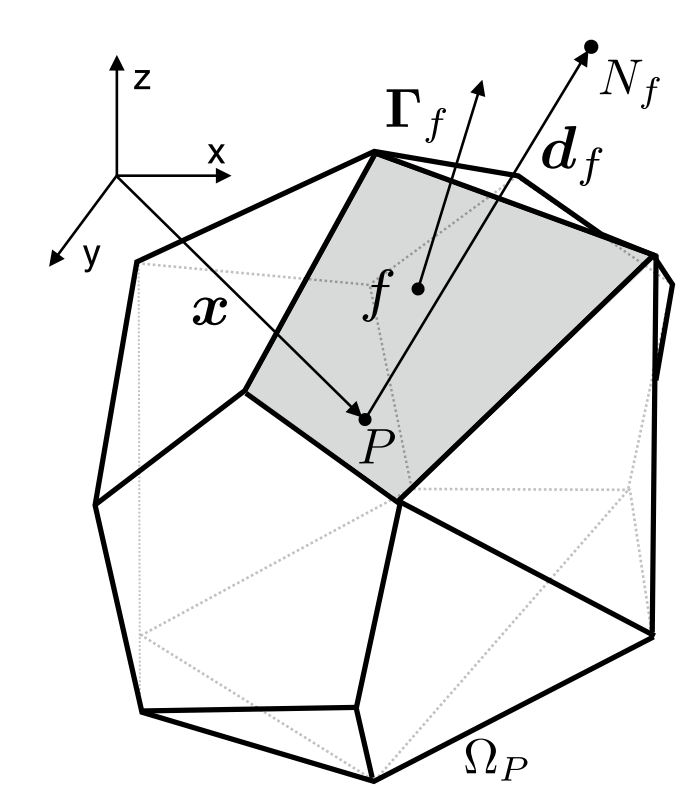
\includegraphics[width=0.3\textwidth]{./figures/controlVolume.png}
%\caption{A polyhedral control volume. Taken from \cite{cardiff2016}}
%\label{fig:finite_volume}
%\end{center}
%\end{figure}

The solution domain is discretised in space and time.
The total specified simulation time is divided into a finite number of time increments $\Delta t$, and the discretised governing momentum equation is solved in a time-marching manner. 

The space domain is divided into a finite number of contiguous convex polyhedral cells.
The proposed solution discretisation follows closely the approach of \citet{cardiff_lagrangian_2017}; consequently, only an overview of the final discretised form of equations and adopted solution algorithm are given below.

%A cell or control volume is shown in Figure \ref{fig:finite volume}. It has the following associated values:
%\begin{itemize}
%	\item A computational node $P$ located at the centre of the cell
%	\item The cell volume $\Omega_{p}$
%	\item The centroid of a neighbouring cell $N$
%	\item Face $f$ with area vector $\mathbf{\Gamma}_f$
%    \item The positional vector of $P$ is $\textbf{r}$
%    \item $P$ and $N$ are joined by the vector $\mathbf{d}_{f}$
%\end{itemize}

To facilitate the use of a segregated solution algorithm, the surface forces term (term on the right-hand side of Equation \ref{eqn:updatedLagFormulation}) is split into explicit and implicit components:
\begin{eqnarray} \label{eqn:MomentumImplicitExplicit}
%	\underbrace{\int_{\Omega_u} \frac{\partial}{\partial t}\left(\rho_u \frac{\partial\left(\boldsymbol{u}^{[m-1]}+\Delta \boldsymbol{u}\right)}{\partial t}\right) \mathrm{d} \Omega_u}_{\text {implicit }}
	\int_{\mathrm{\Omega_u}} \frac{\partial }{\partial t} \left( \rho_u \frac{\partial \mathbf{u} }{\partial t} \right) d\mathrm{\Omega}_u
	&=&
	\underbrace{\oint_{\mathrm{\Gamma}_u}{K_{imp}\  \mathbf{n}_u\cdot\mathrm{\nabla}\left(\mathrm{\Delta \mathbf{u}}\right)}\ d\mathrm{\Gamma}_u}_{\text {implicit }} \notag \\
    &&+
    \underbrace{
    \oint_{\mathrm{\Gamma_u}}(j\mathbf{f}^{-T}\cdot{\mathbf{n}_u)\cdot\boldsymbol{\sigma}}\ d\mathrm{\Gamma_u}
    - 
    \oint_{\mathrm{\Gamma}_u}{K_{imp}\ 
 \mathbf{n}_u\cdot\mathrm{\nabla}\left(\mathrm{\Delta \mathbf{u}}\right)}\ d\mathrm{\Gamma}_u
 }_{\text {explicit }}  %\notag \\
% &&+ \; \mathcal{D}_{\text {Rhie-Chow }} 
\end{eqnarray}
where the first term on the right-hand side (Laplacian term) is treated implicitly, and the second and third terms on the right-hand side are treated explicitly.
Here, by implicit, we mean that the term contributes coefficients to the resulting linear(-ised) system of equations, while the explicit terms will contribute only to the source of the system of linear equations.
The overall procedure will be implicit in time in that the time step size is not constrained by the Courant–Friedrichs–Lewy condition.
This Laplacian term can be considered an approximate compact-stencil linearisation of the surface stress term.
This allows the coupled vector system to be temporarily decoupled in three scalar component equations.
This allows the scalar component equations to be solved independently, where outer Picard iterations provide the inter-component coupling.
Unlike Newton-Raphson approaches, where quadratic convergence may be expected, we can expect linear convergence of the residuals when using a segregated approach; however, this disadvantage is offset in several ways: (i) an exact Jacobian stiffness matrix need not be assembled, which is often costly; (ii) a material tangent is not required for the material laws, as instead the scalar coefficient $K_{imp}$ is only required; (iii) outer Picard iterations are less expensive than Newton iterations as the discretised systems are smaller to assemble and quicker to solve; (iv) Picard iteration may provide superior convergence when the solution is far from the asymptotic region, potentially resulting in a more robust approach for highly nonlinear large strain fracture and damage cases.
Nonetheless, as noted previously \citep{cardiff_block-coupled_2016}, segregated solution procedures can suffer slow convergence relative to coupled approaches, particularly in high aspect ratio linear cases.
In the current work, 
% and third terms on the right-hand side of this equation represent an approximation of the traction field in terms of the displacement field. For this work, the term 
$K_{imp}$ is chosen following the work of \citet{jasak_application_2000} as %which found strong convergence for:
\begin{equation}
	K_{imp} = \frac{4}{3}\mu + \kappa
\end{equation}
where $\mu$ is the material shear modulus and $\kappa$ is the bulk modulus.
It should be reinforced that the value of $K_{imp}$ affects convergence but does not affect the final converged solution, assuming convergence is achieved.

The primary unknown to be solved for is the displacement increment $\Delta \boldsymbol{u}=\boldsymbol{u}^{[m+1]}-\boldsymbol{u}^{[m]}$ where the $[m]$ superscript indicates a quantity from the previous time-step and $[m+1]$ a quantity from the current (to be calculated) time step. 

%Each term of this equation is then discretised as follows (in order):
%\begin{itemize}
%	\item
The resulting conservation equation (Equation \ref{eqn:MomentumImplicitExplicit}) is applied to each cell (control volume) in the computational mesh and discretised in terms of the displacement increment at the cell centre/centroid $(\Delta \mathbf{u})_P$ and at the centres of the neighbouring cells $N_i$.

 The temporal volume integral term is discretised in space using the mid-point rule and discretised in time using a first-order accurate implicit backward Euler scheme \cite{jasak_application_2000}:
% The temporal component containing $\mathbf{u}^{\left[m-1\right]}$ is discretized similarly to what is shown in equation 2.50. However, this term is fully explicit, meaning it only contributes to the source vector in the resulting equation system.
%While it's easy to discretise this temporal term with a second-order accuracy, as demonstrated in the FV method in \citet{jasak_application_2000}, the current elastoplastic method's temporal accuracy is constrained by the first-order backward Euler integration used for the plastic deformation rate for the constitutive law in the models we will encounter throughout this work.
\begin{eqnarray} \label{eq:timeTerm}
	\int_{\mathrm{\Omega_u}} \frac{\partial }{\partial t} \left( \rho_u \frac{\partial (\Delta \mathbf{u}) }{\partial t} \right) d\mathrm{\Omega}_u
	&\approx&
	\frac{\partial }{\partial t} \left( \rho_u \frac{\partial (\Delta \mathbf{u}) }{\partial t} \right)_P \mathrm{\Omega}_P \notag \\
	&\approx&
	\left(
	\frac{ \rho_u^{[m+1]} \frac{\partial (\Delta \mathbf{u}) }{\partial t}^{[m+1]}
	- \rho_u^{[m]} \frac{\partial (\Delta \mathbf{u}) }{\partial t}^{[m]}}{ \Delta t } \right)_P
	\mathrm{\Omega}_P \notag \\
	&\approx&
	\left[
	\frac{ \rho_u^{[m+1]} \left(\frac{\Delta \mathbf{u}^{[m+1]} - \Delta \mathbf{u}^{[m]}}{\Delta t} \right)
	- \rho_u^{[m]} \left(\frac{\Delta \mathbf{u}^{[m]} - \Delta \mathbf{u}^{[m-1]}}{\Delta t} \right)
	}{ \Delta t } 
	\right]_P \mathrm{\Omega}_P \notag \\
	&\approx&
	\frac{1}{\Delta t^2} \left[
	 \rho_{u_P}^{[m+1]} \Delta \mathbf{u}^{[m+1]}_P
	- \left(\rho_{u_P}^{[m+1]} + \rho_{u_P}^{[m]} \right)  \Delta \mathbf{u}^{[m]}_P
	+ \rho_{u_P}^{[m]}  \Delta \mathbf{u}^{[m-1]}_P
	\right]
	 \mathrm{\Omega}_P
%	\int_{\mathrm{\Omega}_u}{\frac{\partial}{\partial t}\left(\rho_u\dot{\mathbf{u} }\right)}d\mathrm{\Omega}_u &\approx&\ \frac{1}{\mathrm{\Delta}t^{\left[m\right]}}\left[\left(\rho_u\mathrm{\Omega}_u\right)_p^{\left[m\right]}\left(\frac{\mathrm{\Delta}\mathbf{u}_P^{\left[m\right]}-\mathrm{\Delta}\mathbf{u}_P^{\left[m-1\right]}}{\mathrm{\Delta}t^{\left[m\right]}}\right)\right. \notag \\
% &&-\left(\rho_u\mathrm{\Omega}_u\right)_p^{\left[m-1\right]}\left.\left(\frac{\mathrm{\Delta}\mathbf{u}_P^{\left[m-1\right]}-\mathrm{\Delta}\mathbf{u}_P^{\left[m-2\right]}}{\mathrm{\Delta}t^{\left[m-1\right]}}\right)\right]
\end{eqnarray}
The $\boldsymbol{u}^{[m-1]}$ term is discretised in a similar fashion, noting that $\boldsymbol{u}^{[m]} = \boldsymbol{u}^{[m-1]} + \Delta \boldsymbol{u}$ in Equation \ref{eqn:MomentumImplicitExplicit}. 

%\item
 The surface forces Laplacian term (first term on the right-hand side of Equation \ref{eqn:MomentumImplicitExplicit}) is discretised using central differencing with over-relaxed non-orthogonal correction \cite{demirdzic_finite_1993, jasak_application_2000, cardiff_development_2014, cardiff_large_2014, cardiff_lagrangian_2017}:
\begin{eqnarray} \label{eq:diffusion}
	\oint_{\mathrm{\Gamma}_u}
	K_{imp} \mathbf{n}_u\cdot\nabla\left(\Delta\mathbf{u}\right) d\mathrm{\Gamma}_u
	&\approx&
	\sum_{f \in N_f} K_{imp}^f \left|\boldsymbol{\Delta}_{u_f}\right|\left(\frac{\Delta \mathbf{u}_{N_f} - \Delta \mathbf{u}_P}{\left|\mathbf{d}_f\right|}\right)\left|\mathbf{\Gamma}_{u_f}\right| \notag \\
	    &&+ \sum_{f \in N_f} K_{imp}^f \; \mathbf{k}_{u_f} \cdot
	    \left[
	    \boldsymbol{\nabla} \left(\mathrm{\Delta}\mathbf{u}\right)
	    \right]_f
	    \left|\mathbf{\Gamma}_{u_f}\right|
\end{eqnarray}
where $N_f$ represents the set of faces $f$ in cell $P$, where neighbouring cell centre $N_f$ shares face $f$ with the cell $P$.
The over-relaxed orthogonal vector $\boldsymbol{\Delta}_{u_f} = \frac{\boldsymbol{d}_{u_f}}{\boldsymbol{d}_{u_f} \cdot \boldsymbol{n}_{u_f}}$ and non-orthogonal correction vector is $\boldsymbol{k}_{u_f}=\boldsymbol{n}_{u_f}-\boldsymbol{\Delta}_{u_f}$, where $\boldsymbol{n}_{u_f}$ is the outward-facing unit normal to the face $f$.
The first term on the right-hand side is treated implicitly, while the second term - representing non-orthogonal corrections at the face - is treated explicitly.

%	\item
 The remaining surface force terms (second and third terms on the right-hand side of Equation \ref{eqn:MomentumImplicitExplicit}) are discretised by assuming that they vary linearly across the face as follows \cite{noauthor_openfoam_2015}:
\begin{equation}
	\oint_{\mathrm{\Gamma_u}}(j\mathbf{f}^{-T}\cdot{\mathbf{n}_u)\cdot\boldsymbol{\sigma}}\ d\mathrm{\Gamma_u}
%	&=& \sum_{F}\int_{\mathrm{\Gamma_{uf}}}(j\mathbf{f}^{-T}\cdot{\mathbf{n}_u)\cdot\boldsymbol{\sigma}}d\Gamma_{uf}
	\approx 
	\sum_{f \in N_f} \mathbf{\Gamma}_{u_f} \cdot
	\left(j\boldsymbol{\sigma}\cdot\mathbf{f}^{-T}\right)_f
\end{equation}
	
\begin{equation} \label{eq:diffusion_exp}
	    \oint_{\mathrm{\Gamma}_u}{K_{imp} \; \mathbf{n}_u\cdot \bb{\nabla} \left(\Delta\mathbf{u}\right)}\ d\mathrm{\Gamma}_u
	    %= 
%	    \sum_{F}\int_{\mathrm{\Gamma}_{uf}}{\left(\frac{4}{3}\mu+K\right)\mathbf{n}_u\cdot\nabla\left(\Delta\mathbf{u}\right)}\ d\mathrm{\Gamma}_{uf}
	\approx
	\sum_{f \in N_f} K_{imp} \; \mathbf{\Gamma}_{u_f} \cdot \left[\bb{\nabla}\left(\mathrm{\Delta}\mathbf{u}\right)\right]_f
\end{equation}

The terms at a face, indicated by the subscript f, are calculated by linearly interpolating from the adjacent cell-centre values. The cell-centre gradients $\bb{\nabla}\left(\mathrm{\Delta}\mathbf{u}\right)$ are determined using a least squares method \cite{noauthor_openfoam_2015}.

%\end{itemize}


%\subsection{Initial and boundary conditions}

All dependent variables must be specified at the initial time.
Boundary conditions must be applied to the faces that coincide with the boundary of the solution domain.
The discretised expressions on boundary faces are modified to account for either the known displacement components in Dirichlet conditions or the known traction for Neumann conditions.
%Mixed condition conditions, such as symmetry planes, treated each component as 
%The expressions for diffusion fluxes and sources remain valid for a Dirichlet boundary condition, but the user-specified boundary value is used in place of the neighbouring cell-centre value.
%On boundaries where Neumann boundary conditions are specified, the boundary fluxes are added to the source term, and the variable values at the boundary are extrapolated from the internal domain using the specified boundary gradient. This process is explained in more detail in \cite{jasak_application_2000}.
Coulomb friction contact boundaries are handled using an iterative penalty method, as described previously \citep{cardiff_lagrangian_2017, cardiff_development_2012}.
More recent segment-to-segment finite volume contact procedures could also be used \citep{Batistic2022, Batistic2023}.
%This method involves measuring the penetration between intersecting cells, calculating penalty forces, and applying them as a Neumann boundary condition. This approach, which was developed for OpenFOAM \cite{cardiff_development_2012}, has also been expanded by the same authors to include the effects of Coulomb friction \cite{cardiff_lagrangian_2017}, which is the friction assumption used in the simulations in this thesis.



\subsubsection{Rhie-Chow Stabilisation}

The difference in the computational stencil for the first and third terms on the right-hand side in Equation \ref{eqn:MomentumImplicitExplicit} introduces third-order numerical diffusion to the discretisation, which quells spurious zero-energy checkerboarding solution oscillations.
First introduced by Rhie and Chow \cite{rhie_numerical_1983} for cell-centred finite volume methods, 
This approach was first proposed for cell-centred solid mechanics procedures by \citet{demirdzic_numerical_1995}, based on the earlier approach of Rhie and Chow \citet{demirdzic_numerical_1995}.
%One issue encountered with the finite volume method is that the discretisation of the governing conservation of momentum equation ( can be unstable and is known to suffer from checker-boarding errors .
%In order to rectify these issues, the Rhie-Chow stabilisation term \cite{rhie_numerical_1983} as introduced into solid mechanics by  is added to the discretised divergence of the stress in equation \ref{eqn:MomentumImplicitExplicit}.
In the current approach, the so-called Rhie-Chow stabilisation term $\mathcal{D}_{\text {Rhie-Chow }}$ takes the following form:
\begin{equation} \label{eq:RhieChow}
	\mathcal{D}_{\text {Rhie-Chow }}
%	&=\sum_{f=1}^{n \text { Faces }}\left\{K_f\left[\left|\boldsymbol{\Delta}_f\right| \frac{\boldsymbol{u}_{N_f}-\boldsymbol{u}_P}{\left|\boldsymbol{d}_f\right|}+\left(\boldsymbol{\Gamma}_f-\boldsymbol{\Delta}_f\right) \cdot(\boldsymbol{\nabla} \boldsymbol{u})_f\right]-\boldsymbol{\Gamma}_f \cdot\left[K_f(\boldsymbol{\nabla} \boldsymbol{u})_f\right]\right\} \\
	= \sum_{f \in N_f} K_{imp}^f
	\left[
	\left|\boldsymbol{\Delta}_f\right| \frac{\Delta \boldsymbol{u}_{N_f} - \Delta \boldsymbol{u}_P}{\left|\boldsymbol{d}_f\right|}
	- \boldsymbol{\Delta}_f \cdot(\boldsymbol{\nabla} (\Delta  \boldsymbol{u}))_f
	\right]
\end{equation}
which comes from the difference between Equations \ref{eq:diffusion} and \ref{eq:diffusion_exp}.
The first term on the right-hand side represents a compact stencil (two-node) approximation of the face normal gradient, while the second term represents a larger stencil approximation.
In the limit of mesh refinement, these two terms cancel out; otherwise, they produce a stabilisation effect which tends to smooth the solution fields.
As the term reduces at a third-order rate, it does not affect the overall scheme's second-order accuracy.

As shown in Section \ref{sec:test_cases}, the magnitude of the Rhie-Chow stabilisation affects the localisation behaviour for damage and fracture mechanics models, with a tendency to artificially \emph{smear out} damage fields.
%In this section, this effect will be explored and quantified.
Two mitigation strategies are proposed here to produce a modified Rhie-Chow stabilisation $\hat{\mathcal{D}}_{\text {Rhie-Chow}}$:
\begin{itemize}
	\item The Rhie-Chow stabilisation is scaled by a global scalar constant $0 \leq \mathcal{R}$ supplied by the user:
	\begin{equation}
		\hat{\mathcal{D}}_{\text{Rhie-Chow}} = \mathcal{R} \; \mathcal{D}_{\text {Rhie-Chow}}
	\end{equation}
	\item The Rhie-Chow stabilisation is scaled by a global scalar constant in addition to a damage-dependent field:
	\begin{equation}
		\hat{\mathcal{D}}_{\text{Rhie-Chow}} = \mathcal{R} (1-D)^2 \; \mathcal{D}_{\text {Rhie-Chow}}
	\end{equation}
\end{itemize}
In the first approach, the smoothing effect is reduced globally with the result that the smearing of damage fields is reduced; however, the disadvantage of this approach is that solution convergence is slowed as the stabilisation term is reduced in magnitude; in addition, numerical oscillations are more likely to appear, particularly in regions undergoing purely elastic deformation where no dissipation mechanisms exist.
In the second approach, a damage variable $0 < D \leq 1$ (to be introduced in Section \ref{sec:constitutive_laws}) reduces the smoothing effect only in regions of damage.
The effect of these proposed modifications are examined in Section \ref{sec:test_cases}.

%\begin{equation}
%\label{eqn:scaleEquation}
%K_f=\mathcal{R} \left(2 \mu+\lambda\right)
%\end{equation}
%where $\mathcal{R}$ is the Rhie-Chow scale factor.

%In order to mitigate the effect of the Rhie-Chow term on the material behaviour, a strategy is proposed in this work whereby the Rhie-Chow scale factor $\mathcal{R}$ in equation \ref{eqn:scaleEquation} is replaced with a field $\mathcal{R}_{field}$ that is a function of the damage field $D$ in the case of the Lemaitre model and the crack variable $d$ in the phase field model. 
%\begin{equation}
%   \mathcal{R}_{field}(D)=(1-D)^2\mathcal{R}
%\end{equation}
%\begin{equation}
%   \mathcal{R}_{field}(d)=(1-d)^2\mathcal{R} 
%\end{equation}


\subsubsection{Hydrostatic Pressure Calculation}
As is well-known, displacement-only formulations are susceptible to displaying numerical hydrostatic pressure oscillations in regions of large isochoric plastic strains.
In \citet{cardiff_lagrangian_2017}, it was proposed to smooth the relative deformation gradient Jacobian field.
In contrast, the current approach forms and solves a pressure Poisson equation:
\begin{equation}
	p = -\frac{\kappa}{2} (J^{2} - 1) + \mathcal{D}_{\text{Rhie-Chow}}^p
\end{equation}
where $p = - \text{tr}(\bb{\sigma})/3$ is the hydrostatic pressure and trace operator is indicated by $\text{tr}(\bullet)$.
The Rhie-Chow pressure stabilisation term $\mathcal{D}_{\text{Rhie-Chow}}^p$ is discretised according to Equation \ref{eq:RhieChow} with the displacement increment $\Delta \bb{u}$ replaced by the pressure $p$.
As in the case of the discretised momentum equation, the magnitude of the Rhie-Chow stabilisation term can be controlled with a global scale constant $0 \leq \mathcal{R}_p$ supplied by the user.
The effect of the Rhie-Chow stabilisation term here is to smooth out any pressure oscillations.
The final form stabilised form of the pressure Poisson equation is 
\begin{equation} \label{eq:pressureEqn}
	p - \mathbb{D} \bb{\nabla}^2 p = -\frac{\kappa}{2} (J^{2} - 1) - \bb{\nabla} \cdot \left( \mathbb{D} \bb{\nabla} p \right)
\end{equation}
where the terms on the left-hand side are discretised implicitly and the terms on the right-hand side are discretised explicitly, following similar methods to Equations \ref{eq:timeTerm} and \ref{eq:diffusion}.
The second terms on the left and right-hand sides come from the Rhie-Chow stabilisation.
The described approach is similar to the formulation proposed by Bijelonja et al. \cite{Bijelonja2002, Bijelonja2005a, Bijelonja2005b, Bijelonja2006} for incompressibility, quasi-incompressibility and elastoplasticity.

\subsection{Solution Algorithm}

The linear momentum equation is discretised for each control volume $P$, and a linear algebraic equation of the following form is assembled \cite{jasak_application_2000}.

\begin{equation}
a_p \Delta \mathbf{u}_p+\sum_F a_n \Delta \mathbf{u}_n=\mathbf{b}_p
\end{equation}

Where $a_{p}$ is the central coefficient, $a_{n}$ are the coefficients associated with the centre of neighbouring cells, $F$ is the number of internal faces of the control volume,  $\mathbf{b}_p$ is the source vector contribution.

These linear algebraic equations are then assembled for all control volumes creating a system of linear algebraic equations:
\begin{equation}
    \mathbf{K}\mathbf{u}=\mathbf{f}
\end{equation}

Where $\mathbf{K}$ is an $M \times M$ coefficient matrix containing the implicit operators where $M$ is the total number of control volumes. The solution vector $\mathbf{u}$ contains the unknown cell-centre displacement increments $\Delta\mathbf{ u}$. $\mathbf{f}$ is the source term containing the explicit operators.
A similar scalar system is formed and solved for the hydrostatic pressure (Equation \ref{eq:pressureEqn}) during the calculation of the stress.

%A segregated solution procedure is employed, where the displacement vector components are solved for separately and sequentially in the $x, y$ and $z$ directions.
As noted in Section \ref{sec:solDomDiscret}, a segregated solution algorithm is employed where the governing vector momentum equation is temporarily decoupled and three scalar equations are solved; outer Picard iterations at each time stpe provide the inter-equation coupling.

%A simple predictor step based on the response of a linear elastic material strained in one dimension is employed (the first term on the RHS of equation \ref{eqn:MomentumImplicitExplicit}).
%In contrast, typical finite element approaches use a Newton-Raphson loop to account for nonlinearities and thus employ the consistent tangent matrix to achieve quadratic convergence \cite{bathe_finite_1996}.
%However, a full, consistent tangent matrix is not easily used in the segregated approach.
%However, a consistent tangent matrix can also be difficult to calculate in the damage and fracture models, and convergence difficulties can be encountered.
%The current method employs Picard/FixedPoint iterations to account for the nonlinearities and hence does not require a consistent tangent matrix.
%Outer iterations are performed to account for the inter-equation coupling and the linearized nonlinear terms.
The \emph{inner} linear sparse system is iteratively solved using an incomplete Cholesky pre-conditioned conjugate gradient method \cite{jacobs_generalization_1986}.
%In non-linear problems, this system of equations is solved multiple times with updated coefficients in a fixed-point iteration scheme. 
As noted in previous articles on segregated methods, the inner system need not be solved to a tight tolerance as coefficients and source terms are approximated from the previous increment; a reduction in the residuals of one order of magnitude is typically sufficient. The outer iterations are performed until the predefined tolerance, typically $1 \times 10^{-6}$, has been achieved \cite{cardiff_lagrangian_2017}. 

In the current updated Lagrangian approach, the mesh is moved to the deformed configuration at the end of each time step.
Given that the displacements are calculated at the cell centres, interpolation must be performed to calculate the displacements at the vertices to update the mesh. A linear least-squared method is employed here \cite{cardiff_lagrangian_2017}.
%In this method, a linear least squares plane is fit through a vertex and its immediately adjacent cell centres. For boundary vertices, boundary face-centre values are also included in the fitting.

The procedures have been implemented and publicly shared within the solids4foam toolbox \citep{Cardiff2018, Tukovic2018} of the open-source OpenFOAM software.

An overview of the solution algorithm is shown in Algorithm \ref{alg:solAlg}.
 
\begin{algorithm}[htb] \label{alg:solAlg}
\SetAlgoLined
\text{\textbf{for all} time steps \textbf{do}} \\
\ \ \text{       \textbf{while} convergence not reached \textbf{do}} 
\ \text{       - Discrete governing system (Equation 4) for each cell, using Equations 5-10, in terms of $\Delta\mathbf{u}$}
\ \text{       - Assemble the discretised  equations for all cells into three scalar linear systems (Equation 14)}
\ \text{       - Solve the three scalar linear systems in terms of cell-centred displacement increments $\Delta\mathbf{u}$}
\  \text{      - Update/reconstruct the kinematics: $\bb{\nabla}(\bb{\Delta} \bb{u})$, $\bb{F}$, $J$, $\bb{f}$, $j$ } \\
\  \text{      - Update the stress ($\bb{\sigma}$) at the cell-centres using the chosen material law} \\
\  \text{      - Update the Rhie-Chow stabilisation: $\hat{\mathcal{D}}_{\text{Rhie-Chow}}$ } \\
\ \ \text{       \textbf{end while}}
\ \ \text{      - Interpolate cell-centre displacement increments to the vertices}
\ \ \text{      - Move mesh to the deformed configuration using the vertex displacements, incorporating}
\ \ \text{        layer addition/removal (Section 2.4)}
 \caption{Solution Procedure}
\text{\textbf{end for}}
\end{algorithm}


\subsection{Eulerian-Type Layer Addition and Removal Boundaries} \label{sec:euler_BCs}

Steady-state behaviour is typically the primary interest in wire drawing and other continuous forming approaches.
Eulerian approaches are a natural choice but are not commonly employed when elastic phenomena (e.g. spring back, residual stresses) are important.
When simulating wire drawing using a Lagrangian approach, a na\"ive approach is to simulate a workpiece segment that is \emph{long enough} to allow steady-state to be reached.
The disadvantage of this approach is that computational cost is inflated by the portion of the workpiece domain primarily undergoing rigid-body translation, which may be large relative to the region undergoing plastic deformations.

To overcome this disadvantage, the current work proposes Eulerian-type layer addition and removal conditions for the workpiece upstream and downstream boundaries.
The approach involves fixing the workpiece (e.g., wire) upstream and downstream mesh boundaries in space during the mesh motion at the end of each time step.
As cells near the upstream boundary become elongated, layers of new cells are added.
Similarly, cells are removed as they become compressed near the downstream patch.
In this way, the length of the workpiece domain remains fixed (like an Eulerian approach), but a traditional Lagrangian method is still used to calculate the deformation.

Figure \ref{fig:layerAddition} schematically outlines the step involved in the layer addition and removal mesh motion scheme:
\begin{enumerate}[label=(\alph*)]
	\item The workpiece (e.g., wire) mesh is constructed such that it is layered in the streamwise direction;
	\item Solution of the discretised governing equations provides the cell centres displacement increments $\Delta \bb{u}$;
	\item The cell-centred displacement increment $\Delta \bb{u}$ are interpolated to the vertices $\Delta \bb{u}_v$;
	\item If the average width (in the streamwise direction) of the cell layer $d_{av}$ is greater at the upsrteam boundary than a user-prescribed maximum width $d_{max}$, a zero-thickness layer of cells at the upstream boundary. The displacement increments of the newly added layer of vertices are taken from the upstream boundary vertices;
	\item The vertex displacement increments $\Delta \bb{u}_v$ at the upstream and downstream boundaries are set to zero, except for the newly added vertices part of the zero-thickness layer;
	\item The mesh is moved by the vertex displacement increment field $\Delta \bb{u}_v$, where it is noted that the vertices on the upstream and downstream points do not move;
	\item If the average width (in the streamwise direction) of the cell layer $d_{av}$ at the downstream boundary is less than a user-prescribed minimum width $d_{min}$, remove the layer of cells at the downstream boundary. Depending on displacement increment magnitude, multiple cell layers may need to be removed.
\end{enumerate}

\begin{figure}[tbh]
	\centering
	\subfigure[] {\label{airbus}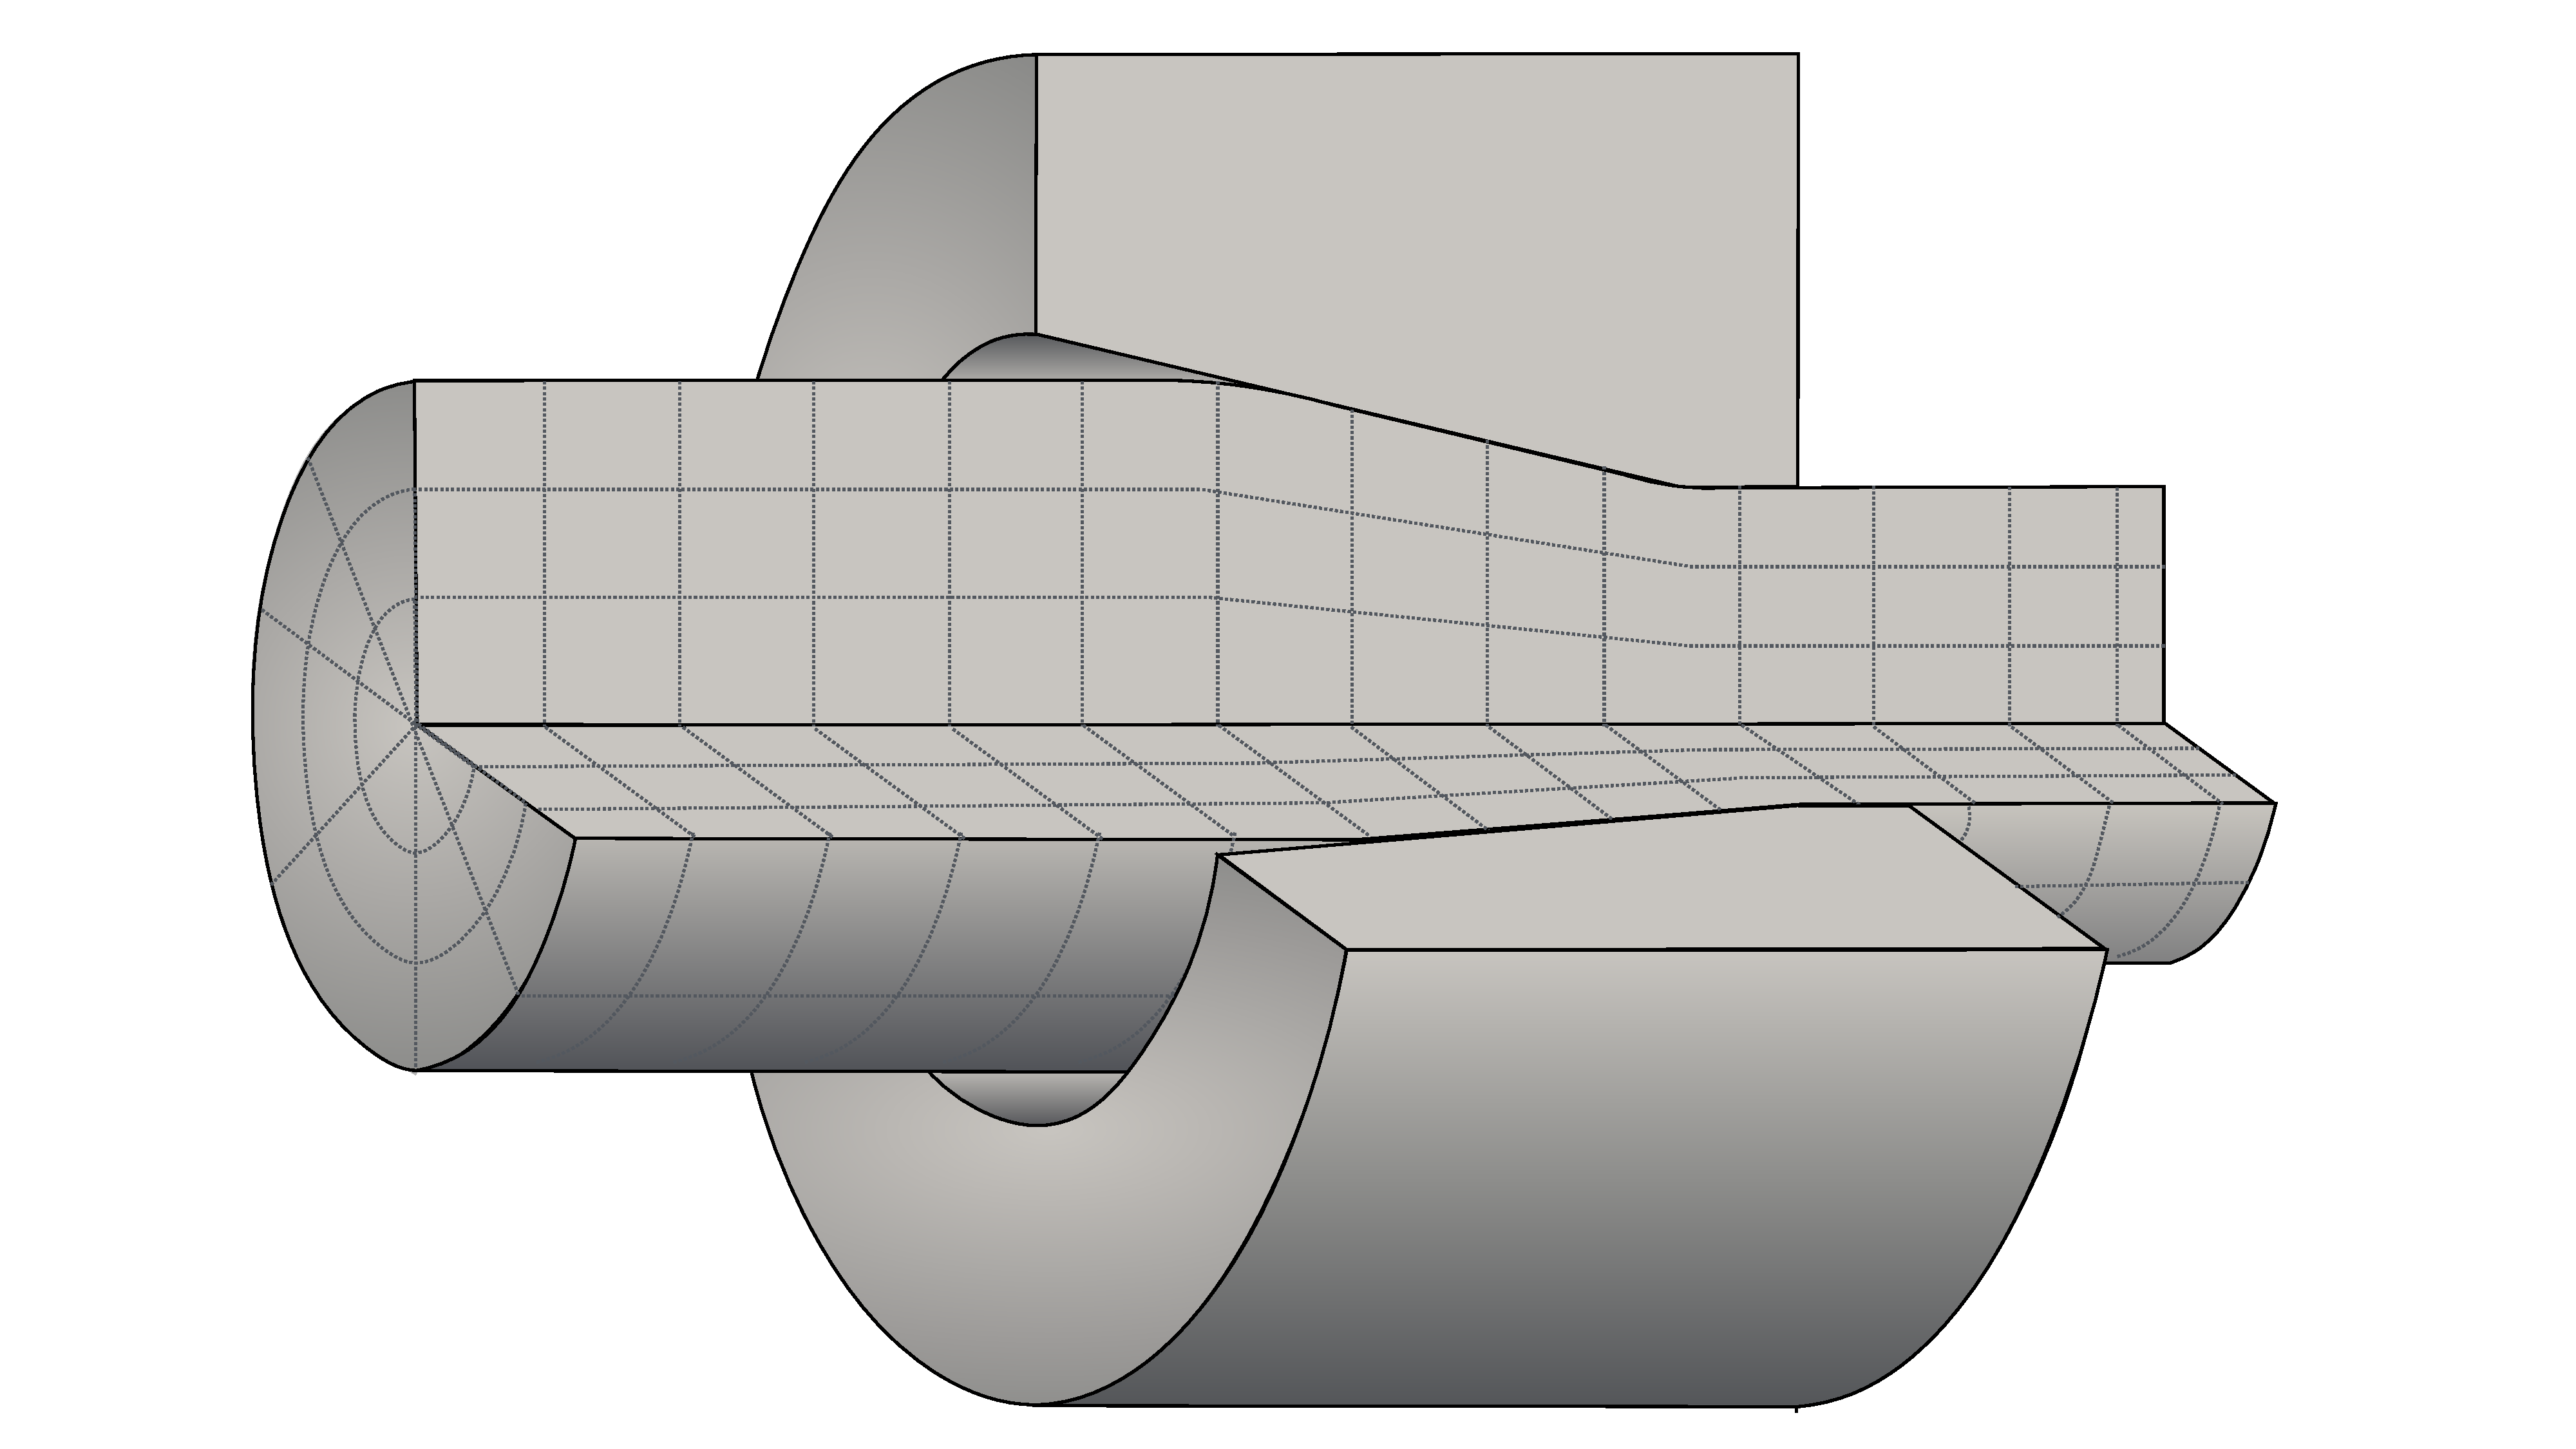
\includegraphics[width=0.3\textwidth]{./Figures/layerAddition/fig1}}
	\subfigure[] {\label{airbus}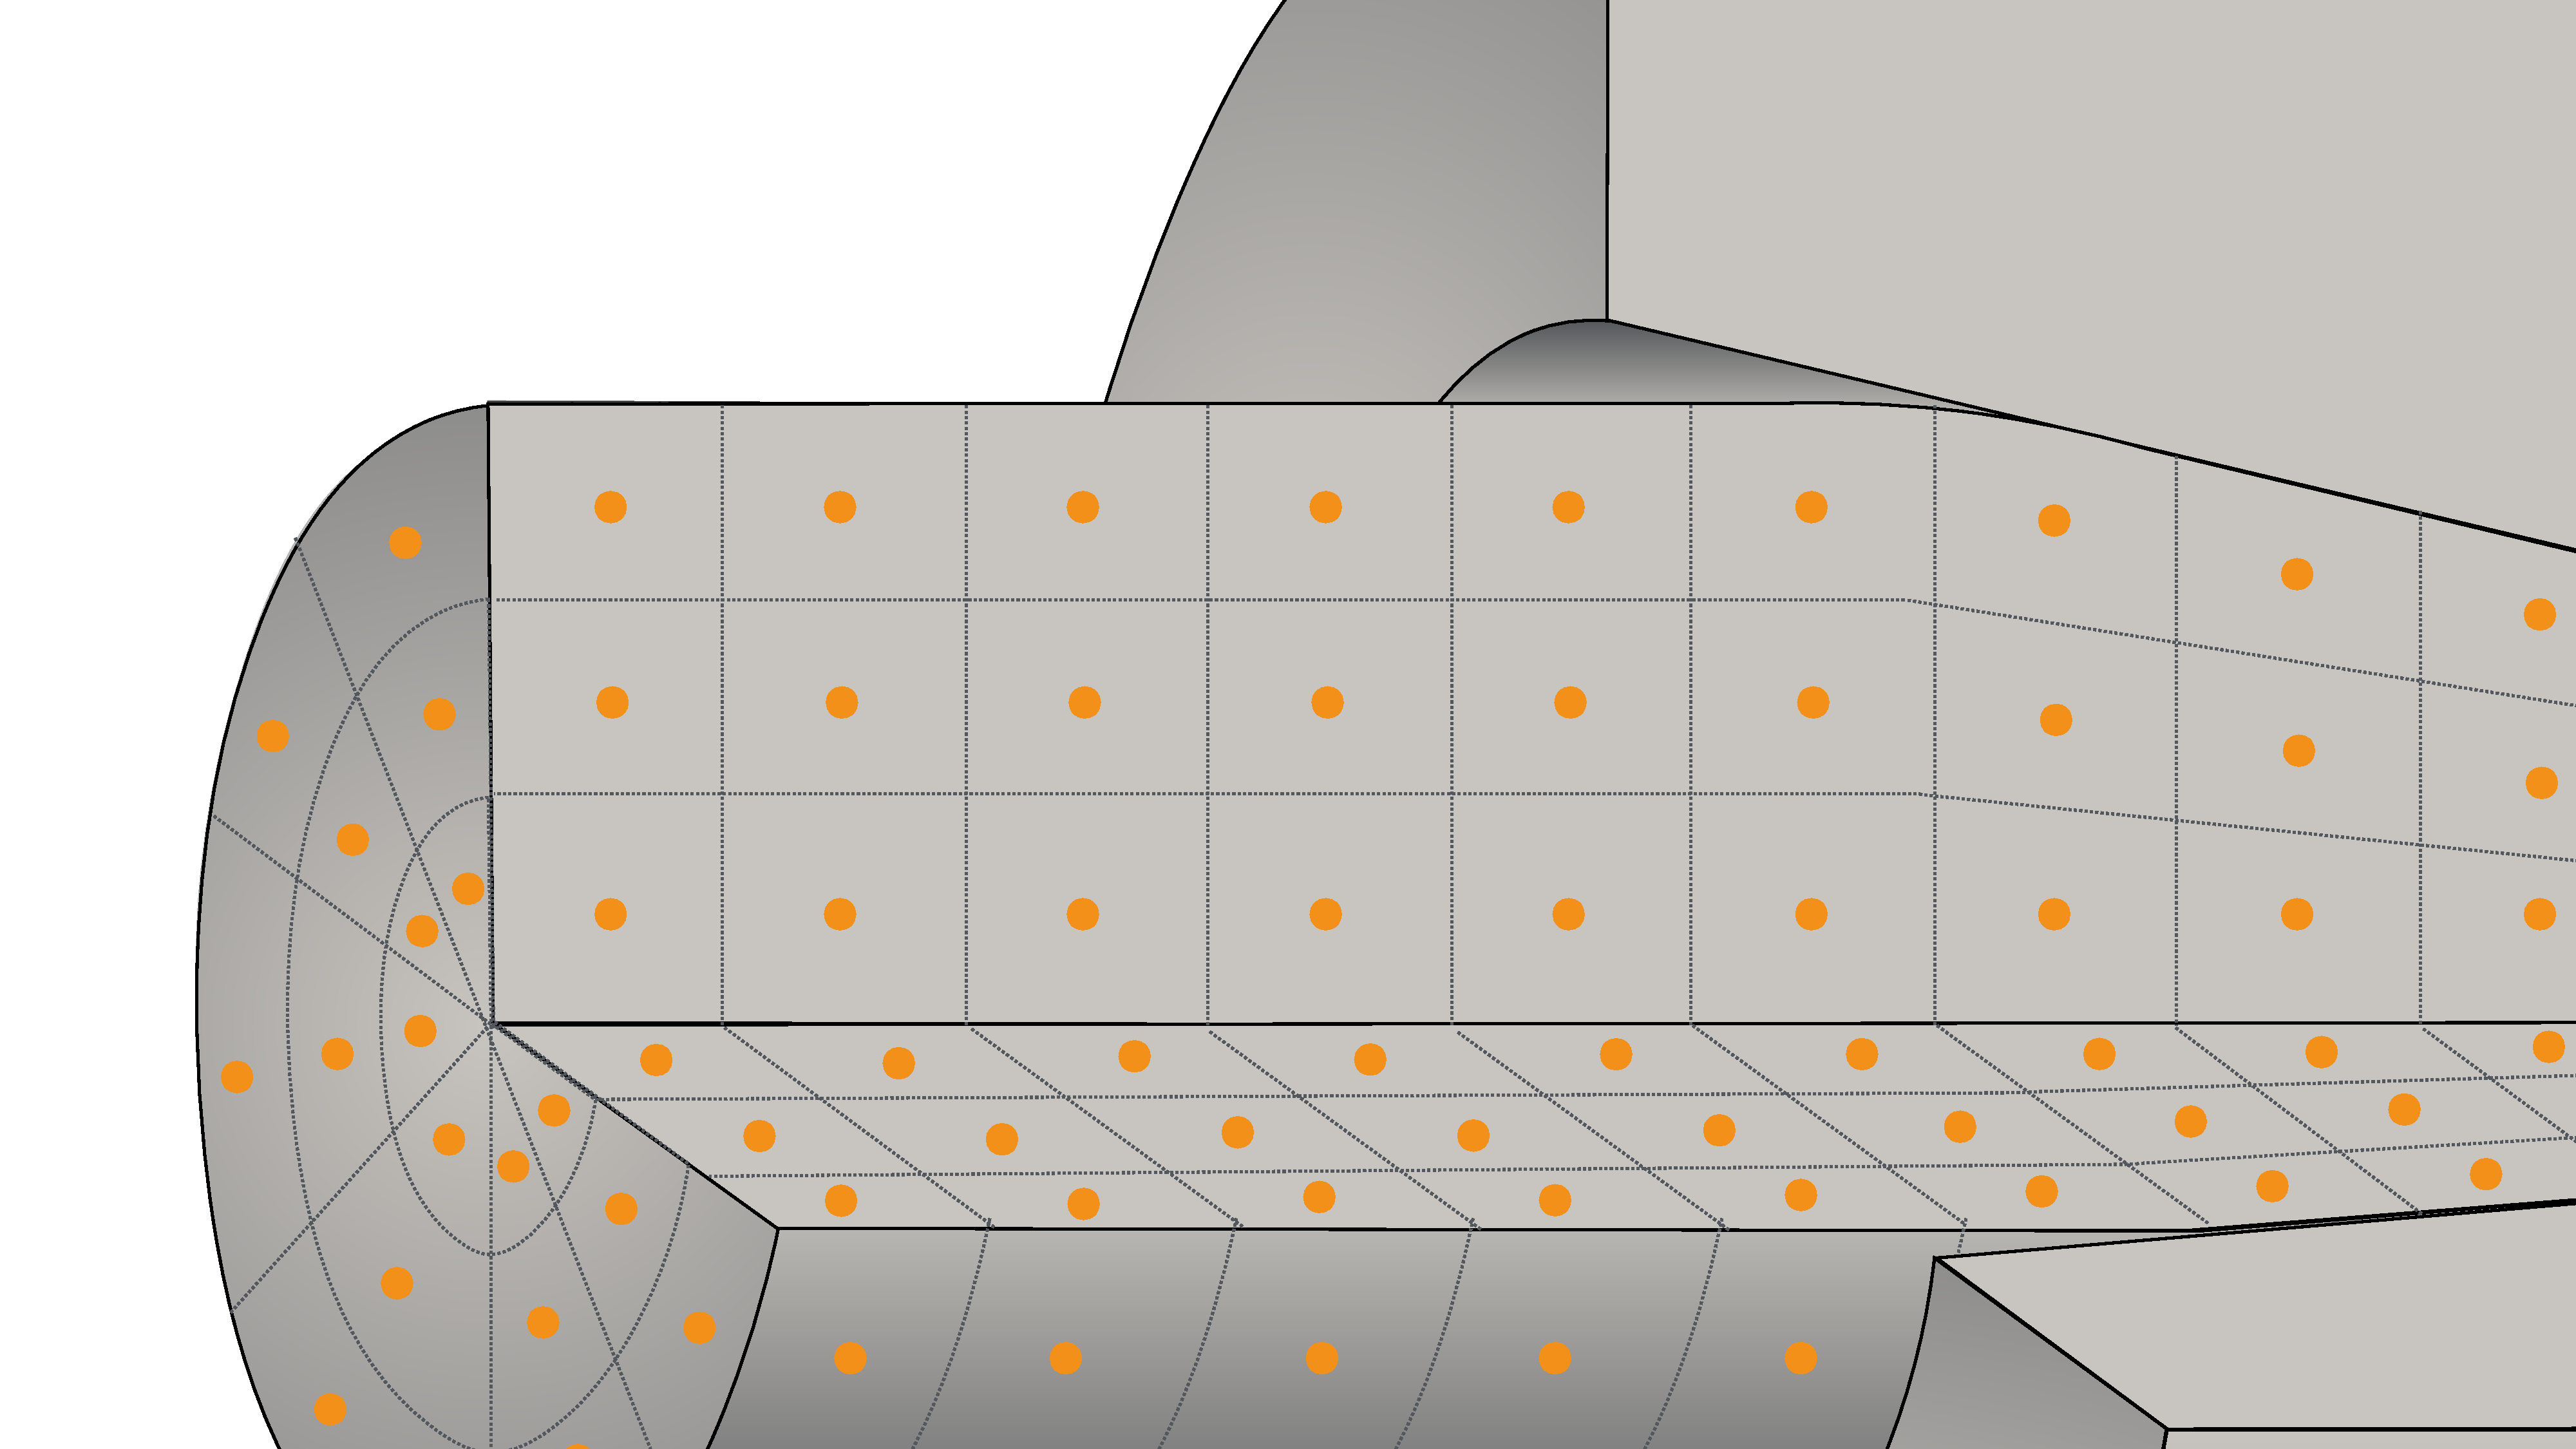
\includegraphics[width=0.3\textwidth]{./Figures/layerAddition/fig2}}
	\subfigure[] {\label{airbus}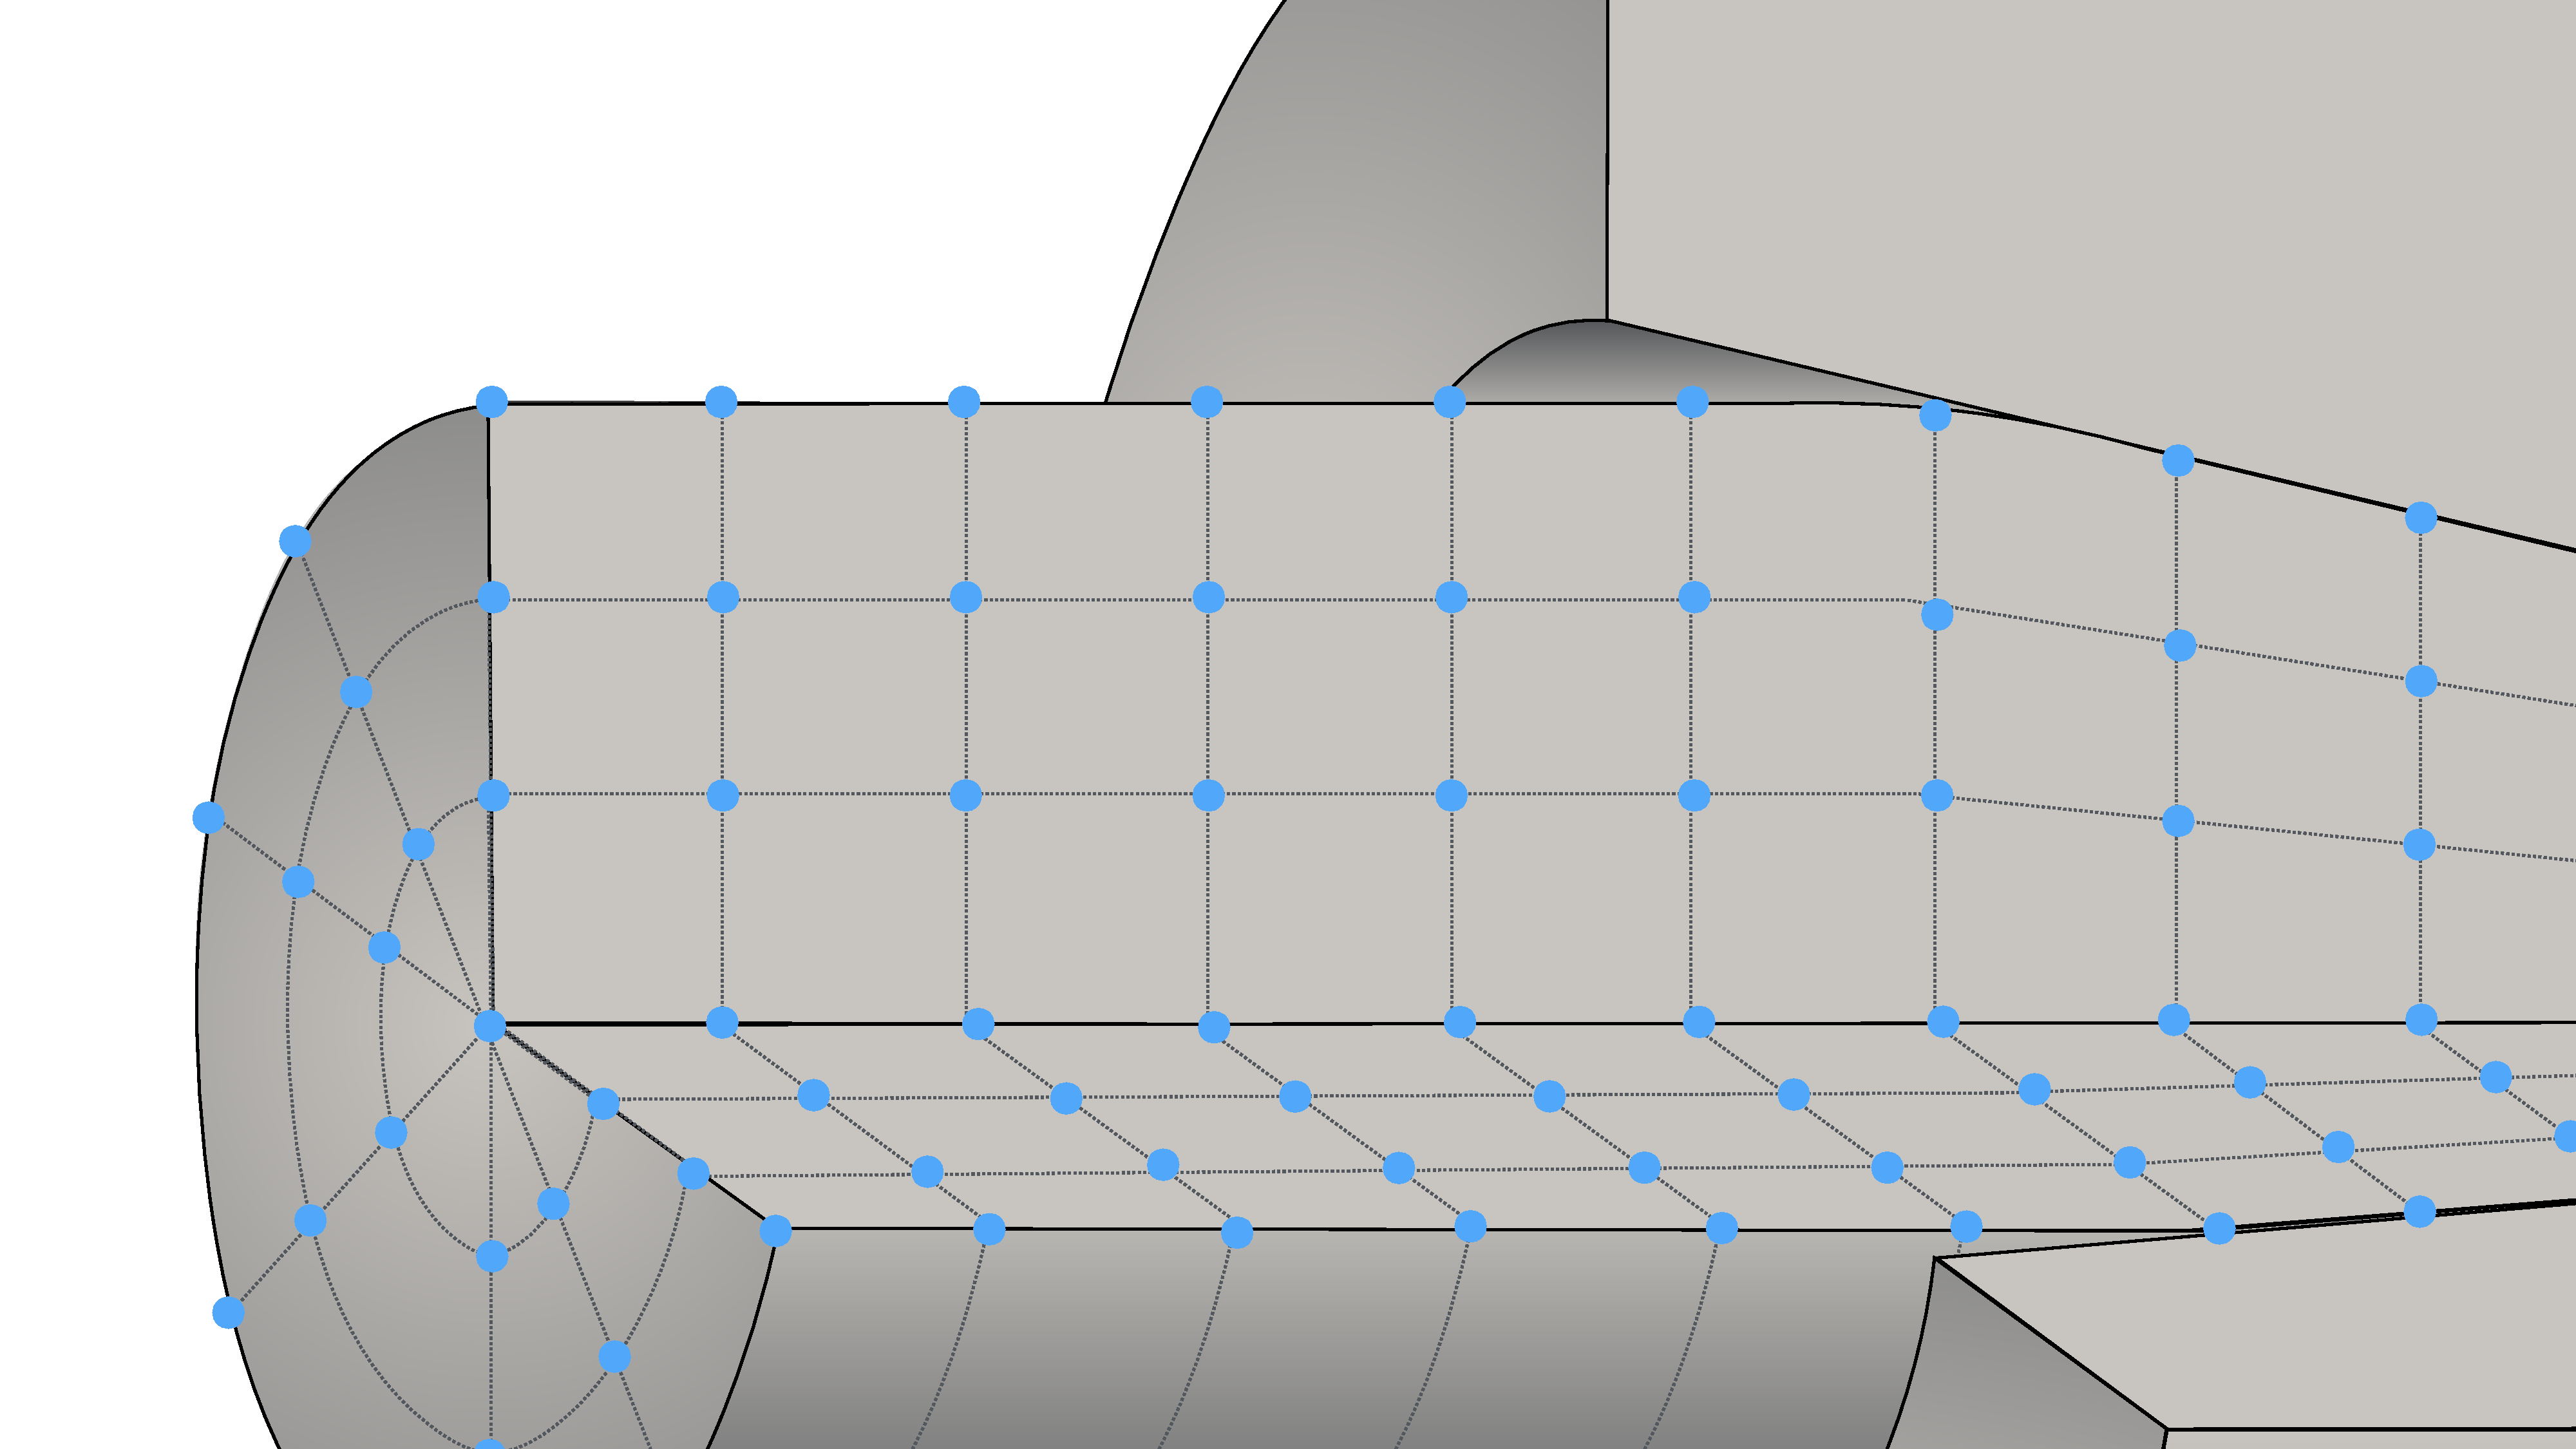
\includegraphics[width=0.3\textwidth]{./Figures/layerAddition/fig3}}
	\subfigure[] {\label{airbus}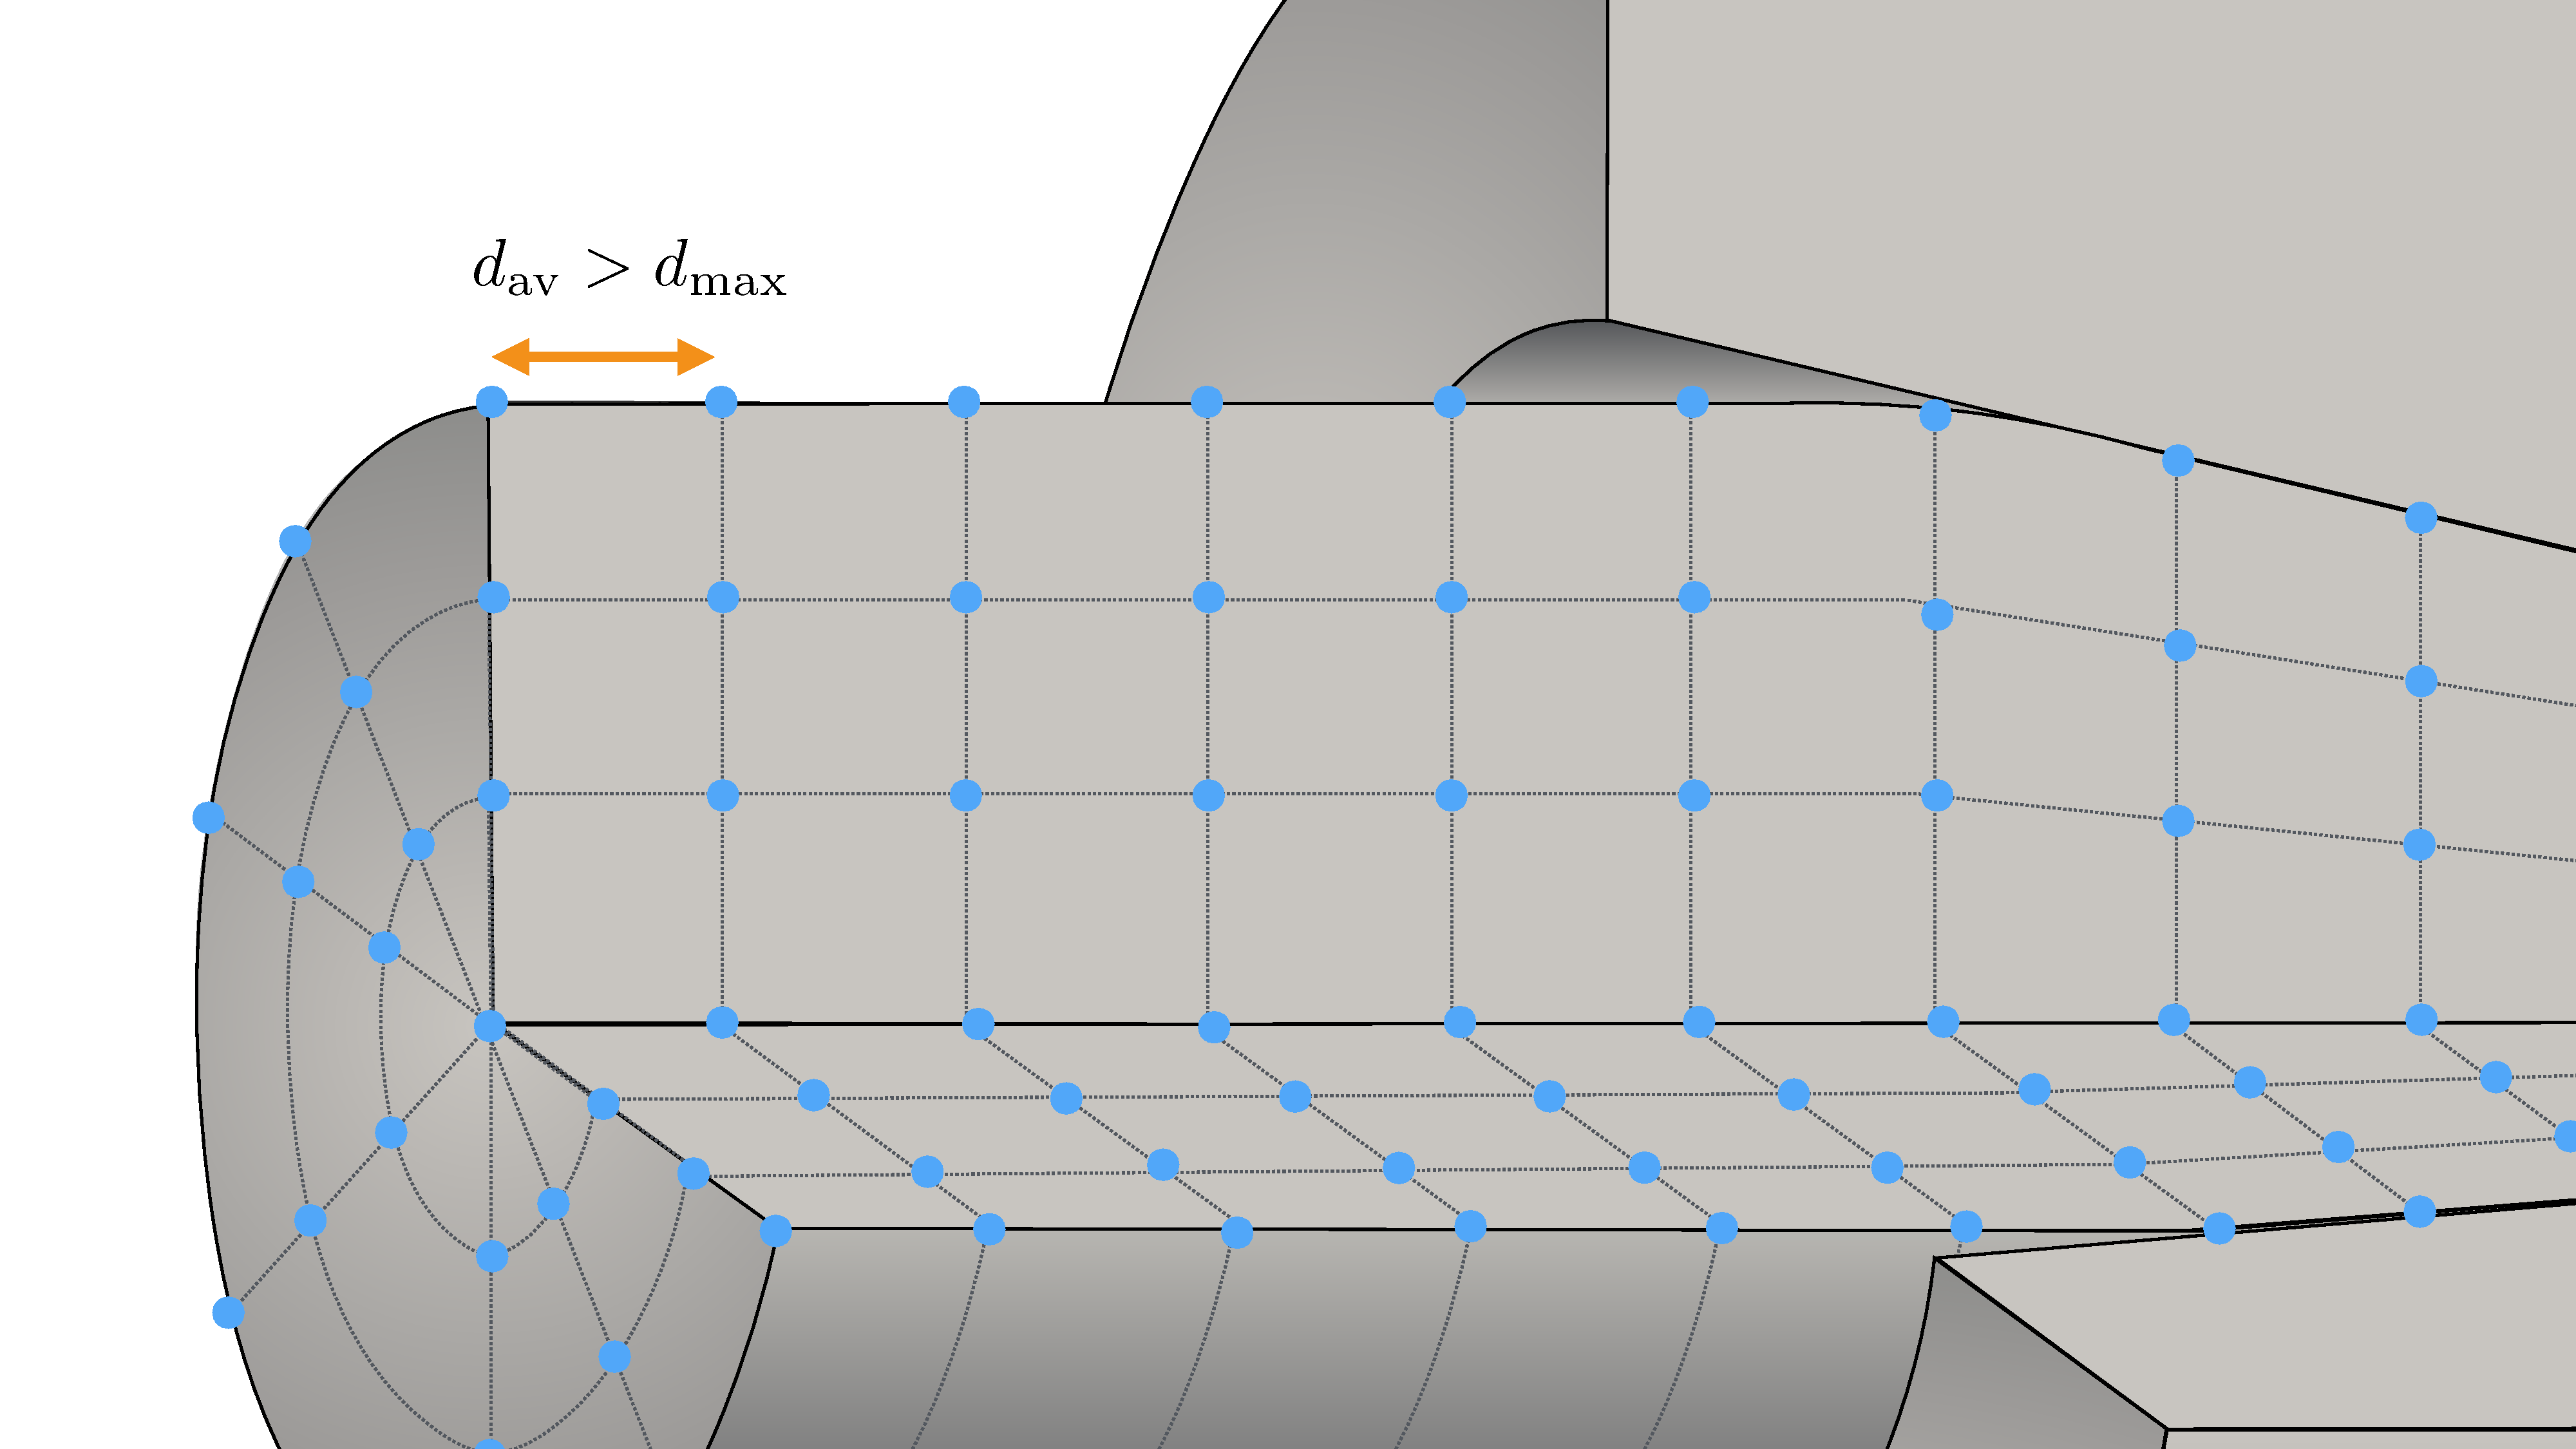
\includegraphics[width=0.3\textwidth]{./Figures/layerAddition/fig4}}
	\subfigure[] {\label{airbus}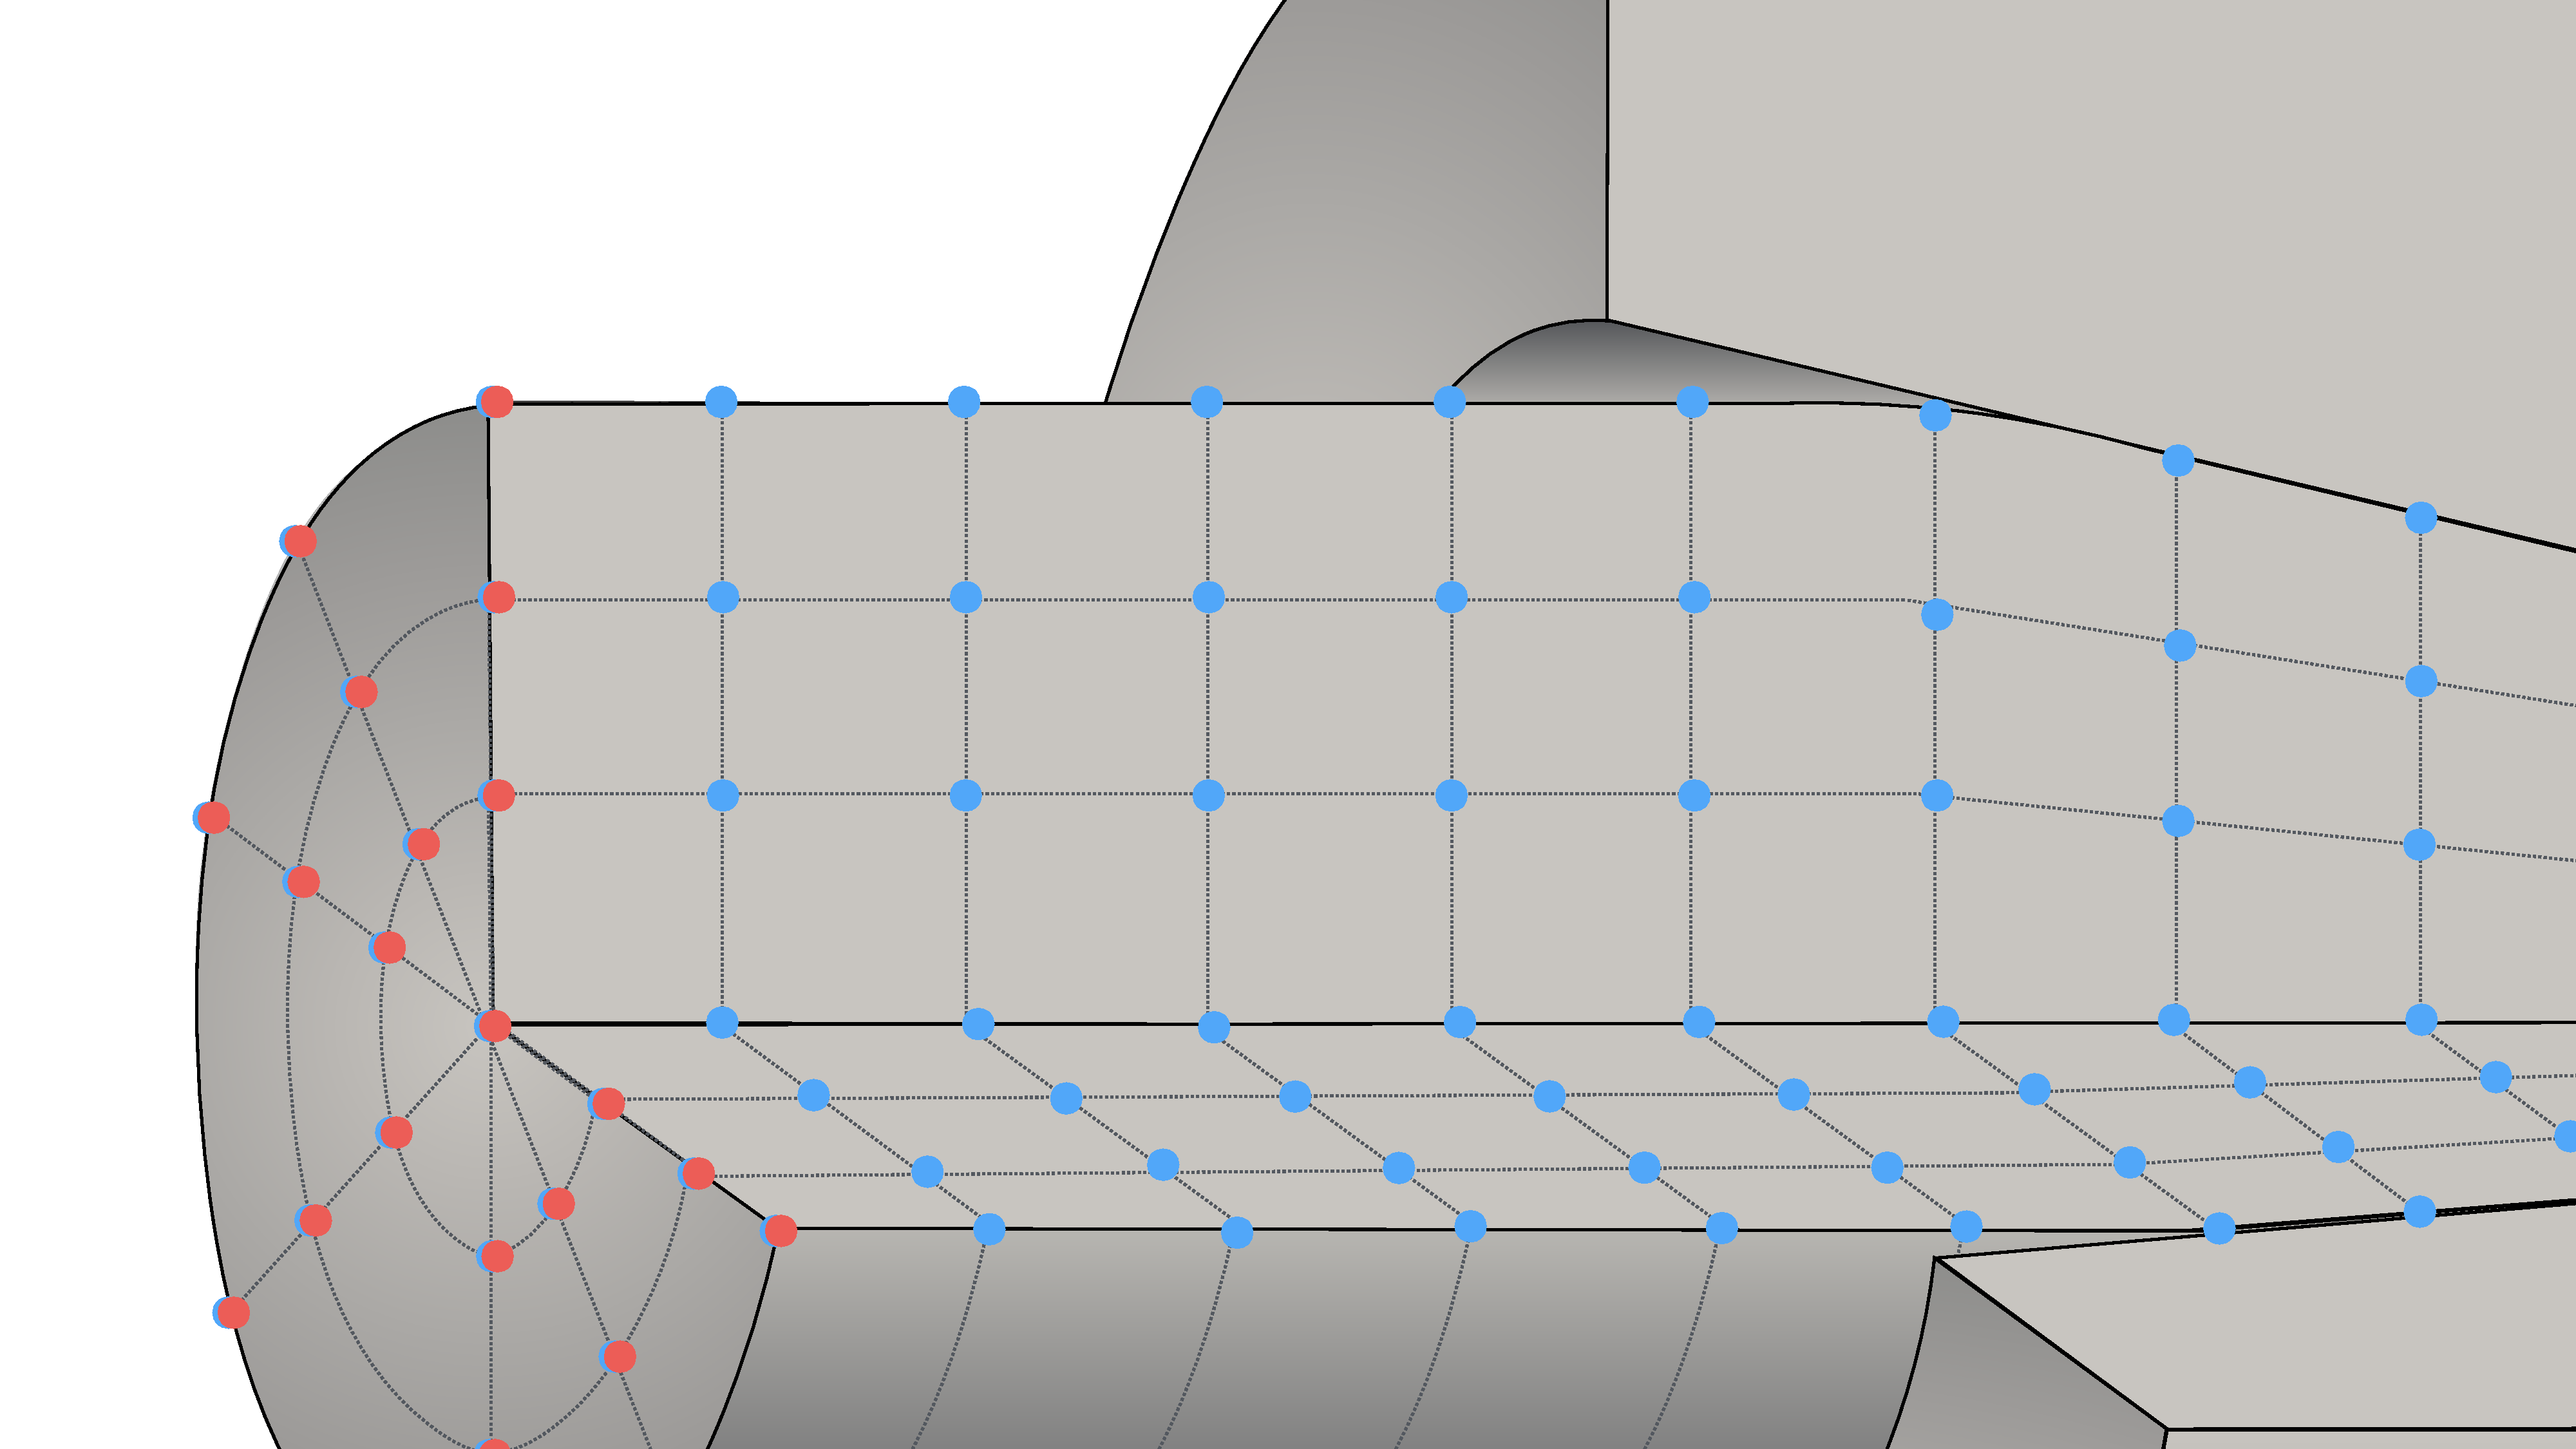
\includegraphics[width=0.3\textwidth]{./Figures/layerAddition/fig5}}
	\subfigure[] {\label{airbus}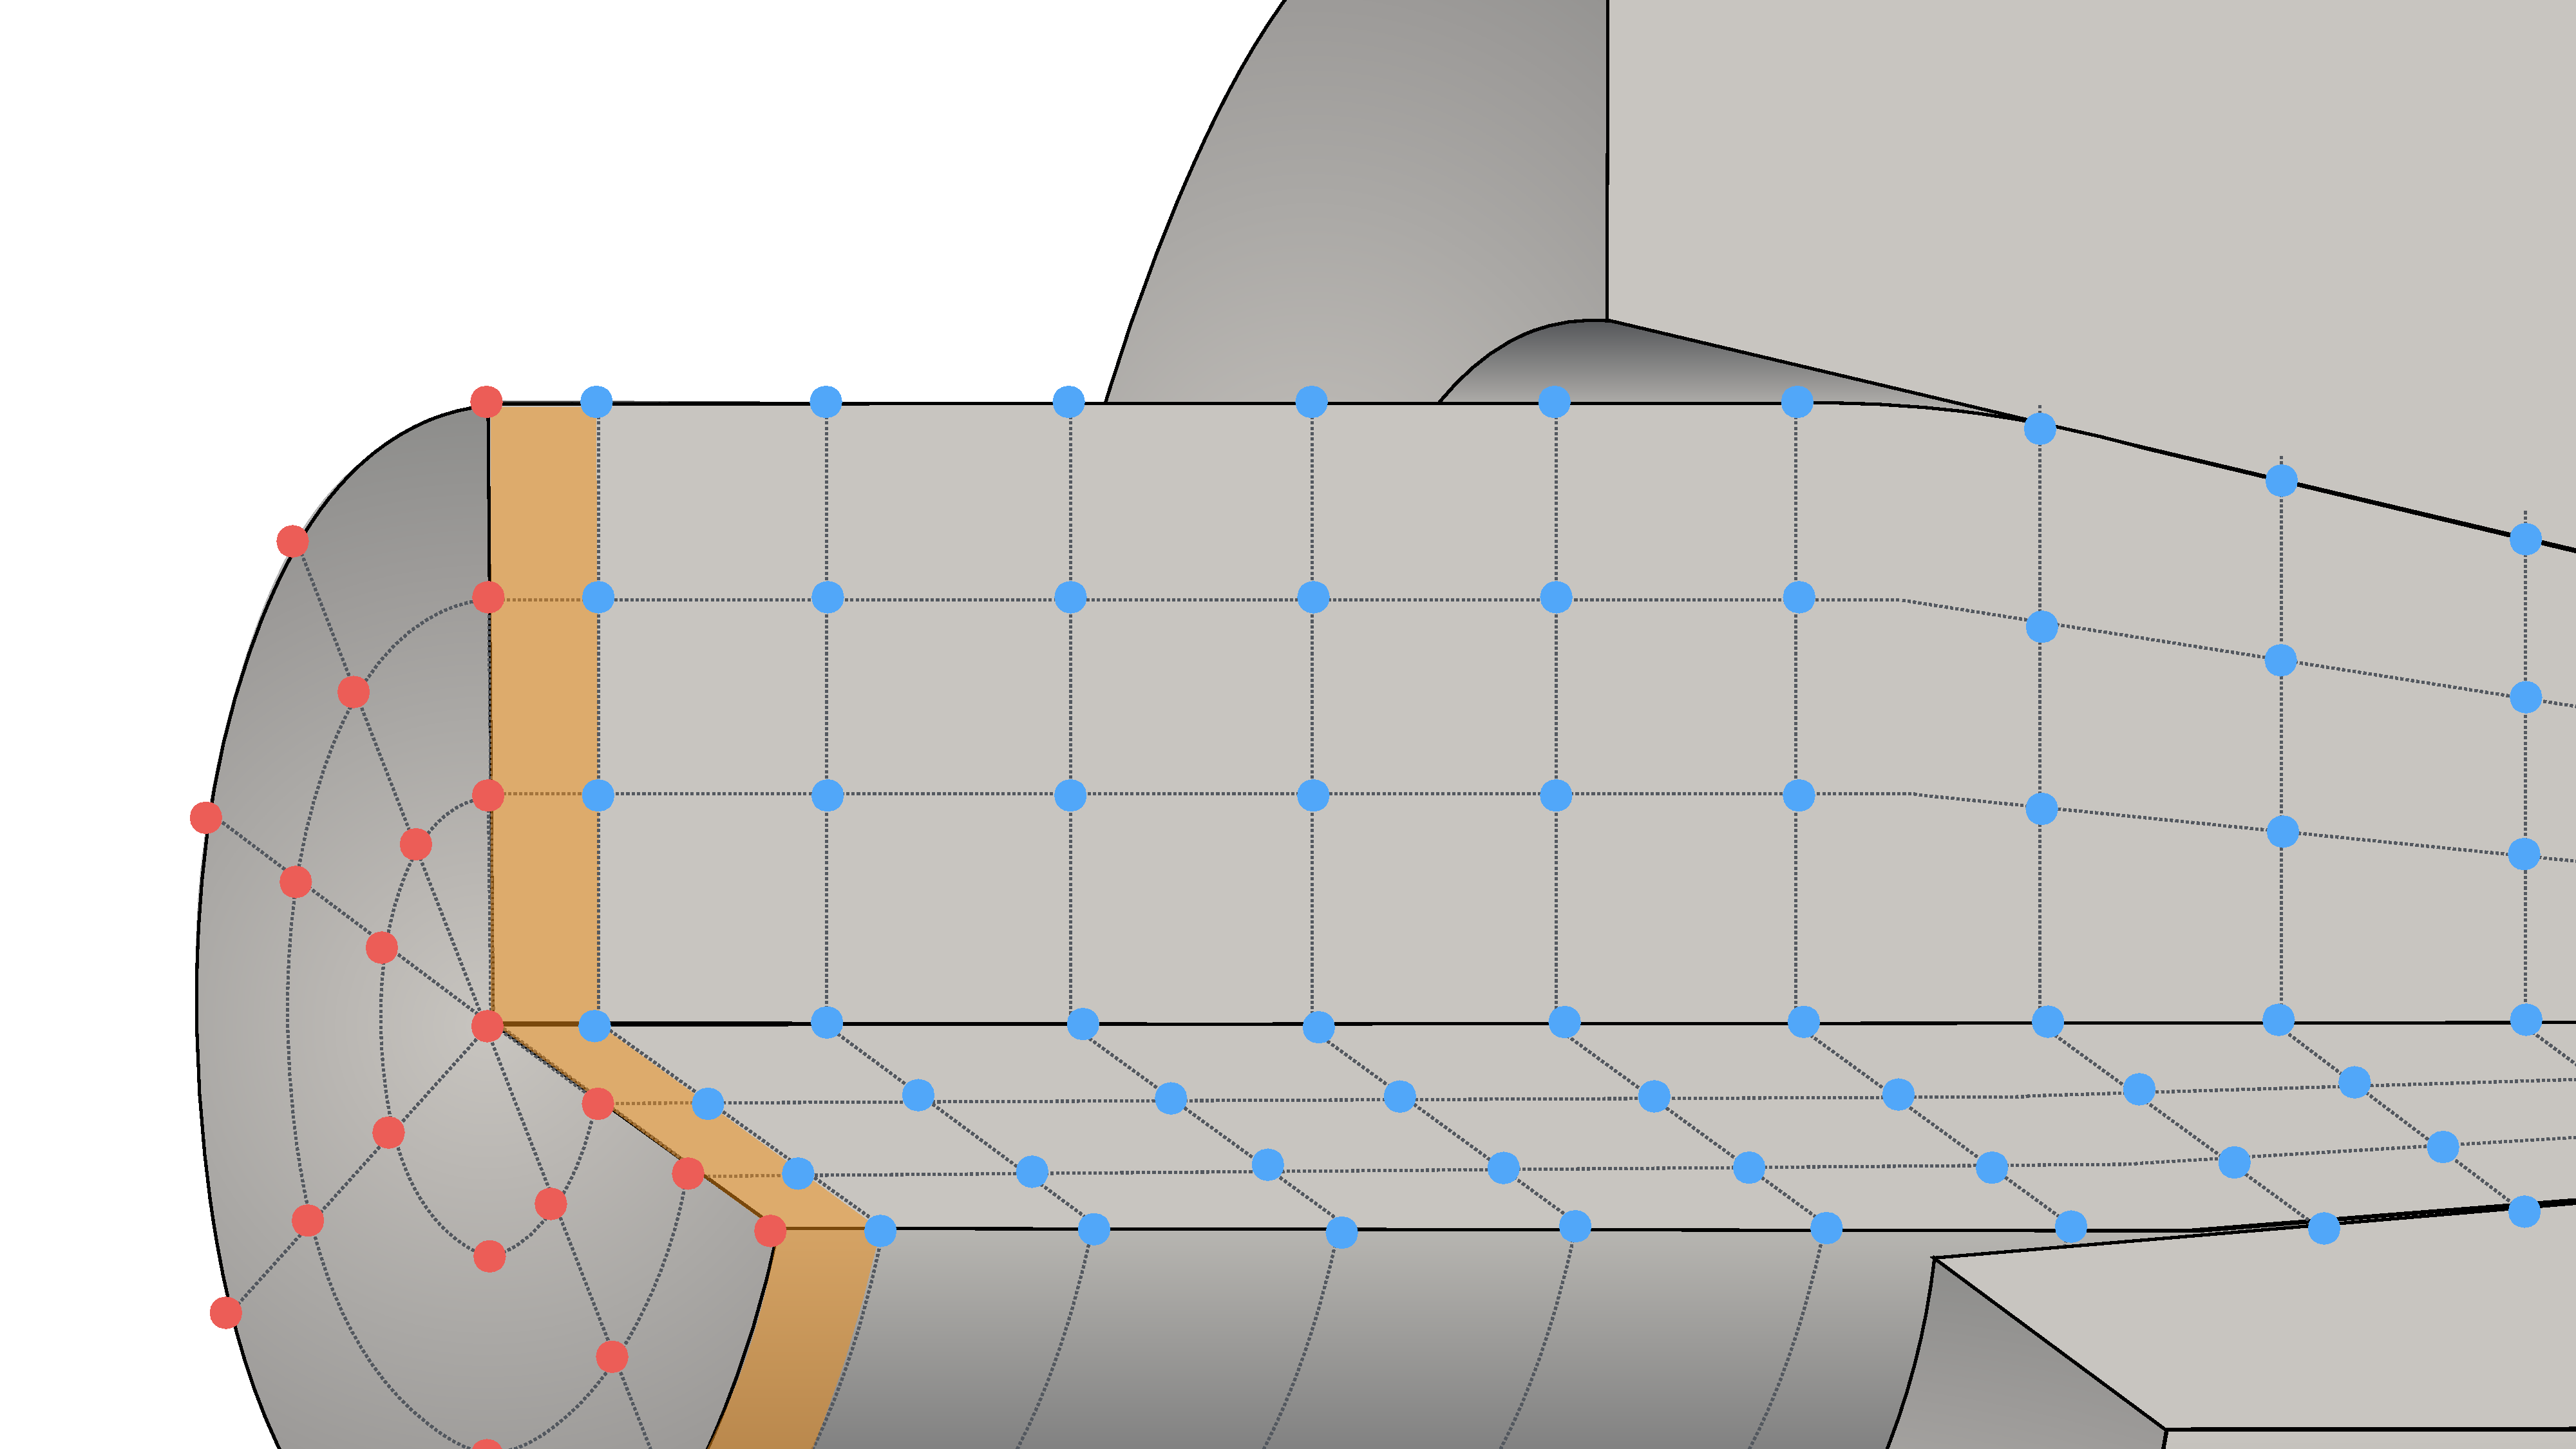
\includegraphics[width=0.3\textwidth]{./Figures/layerAddition/fig6}}
	\subfigure[] {\label{airbus}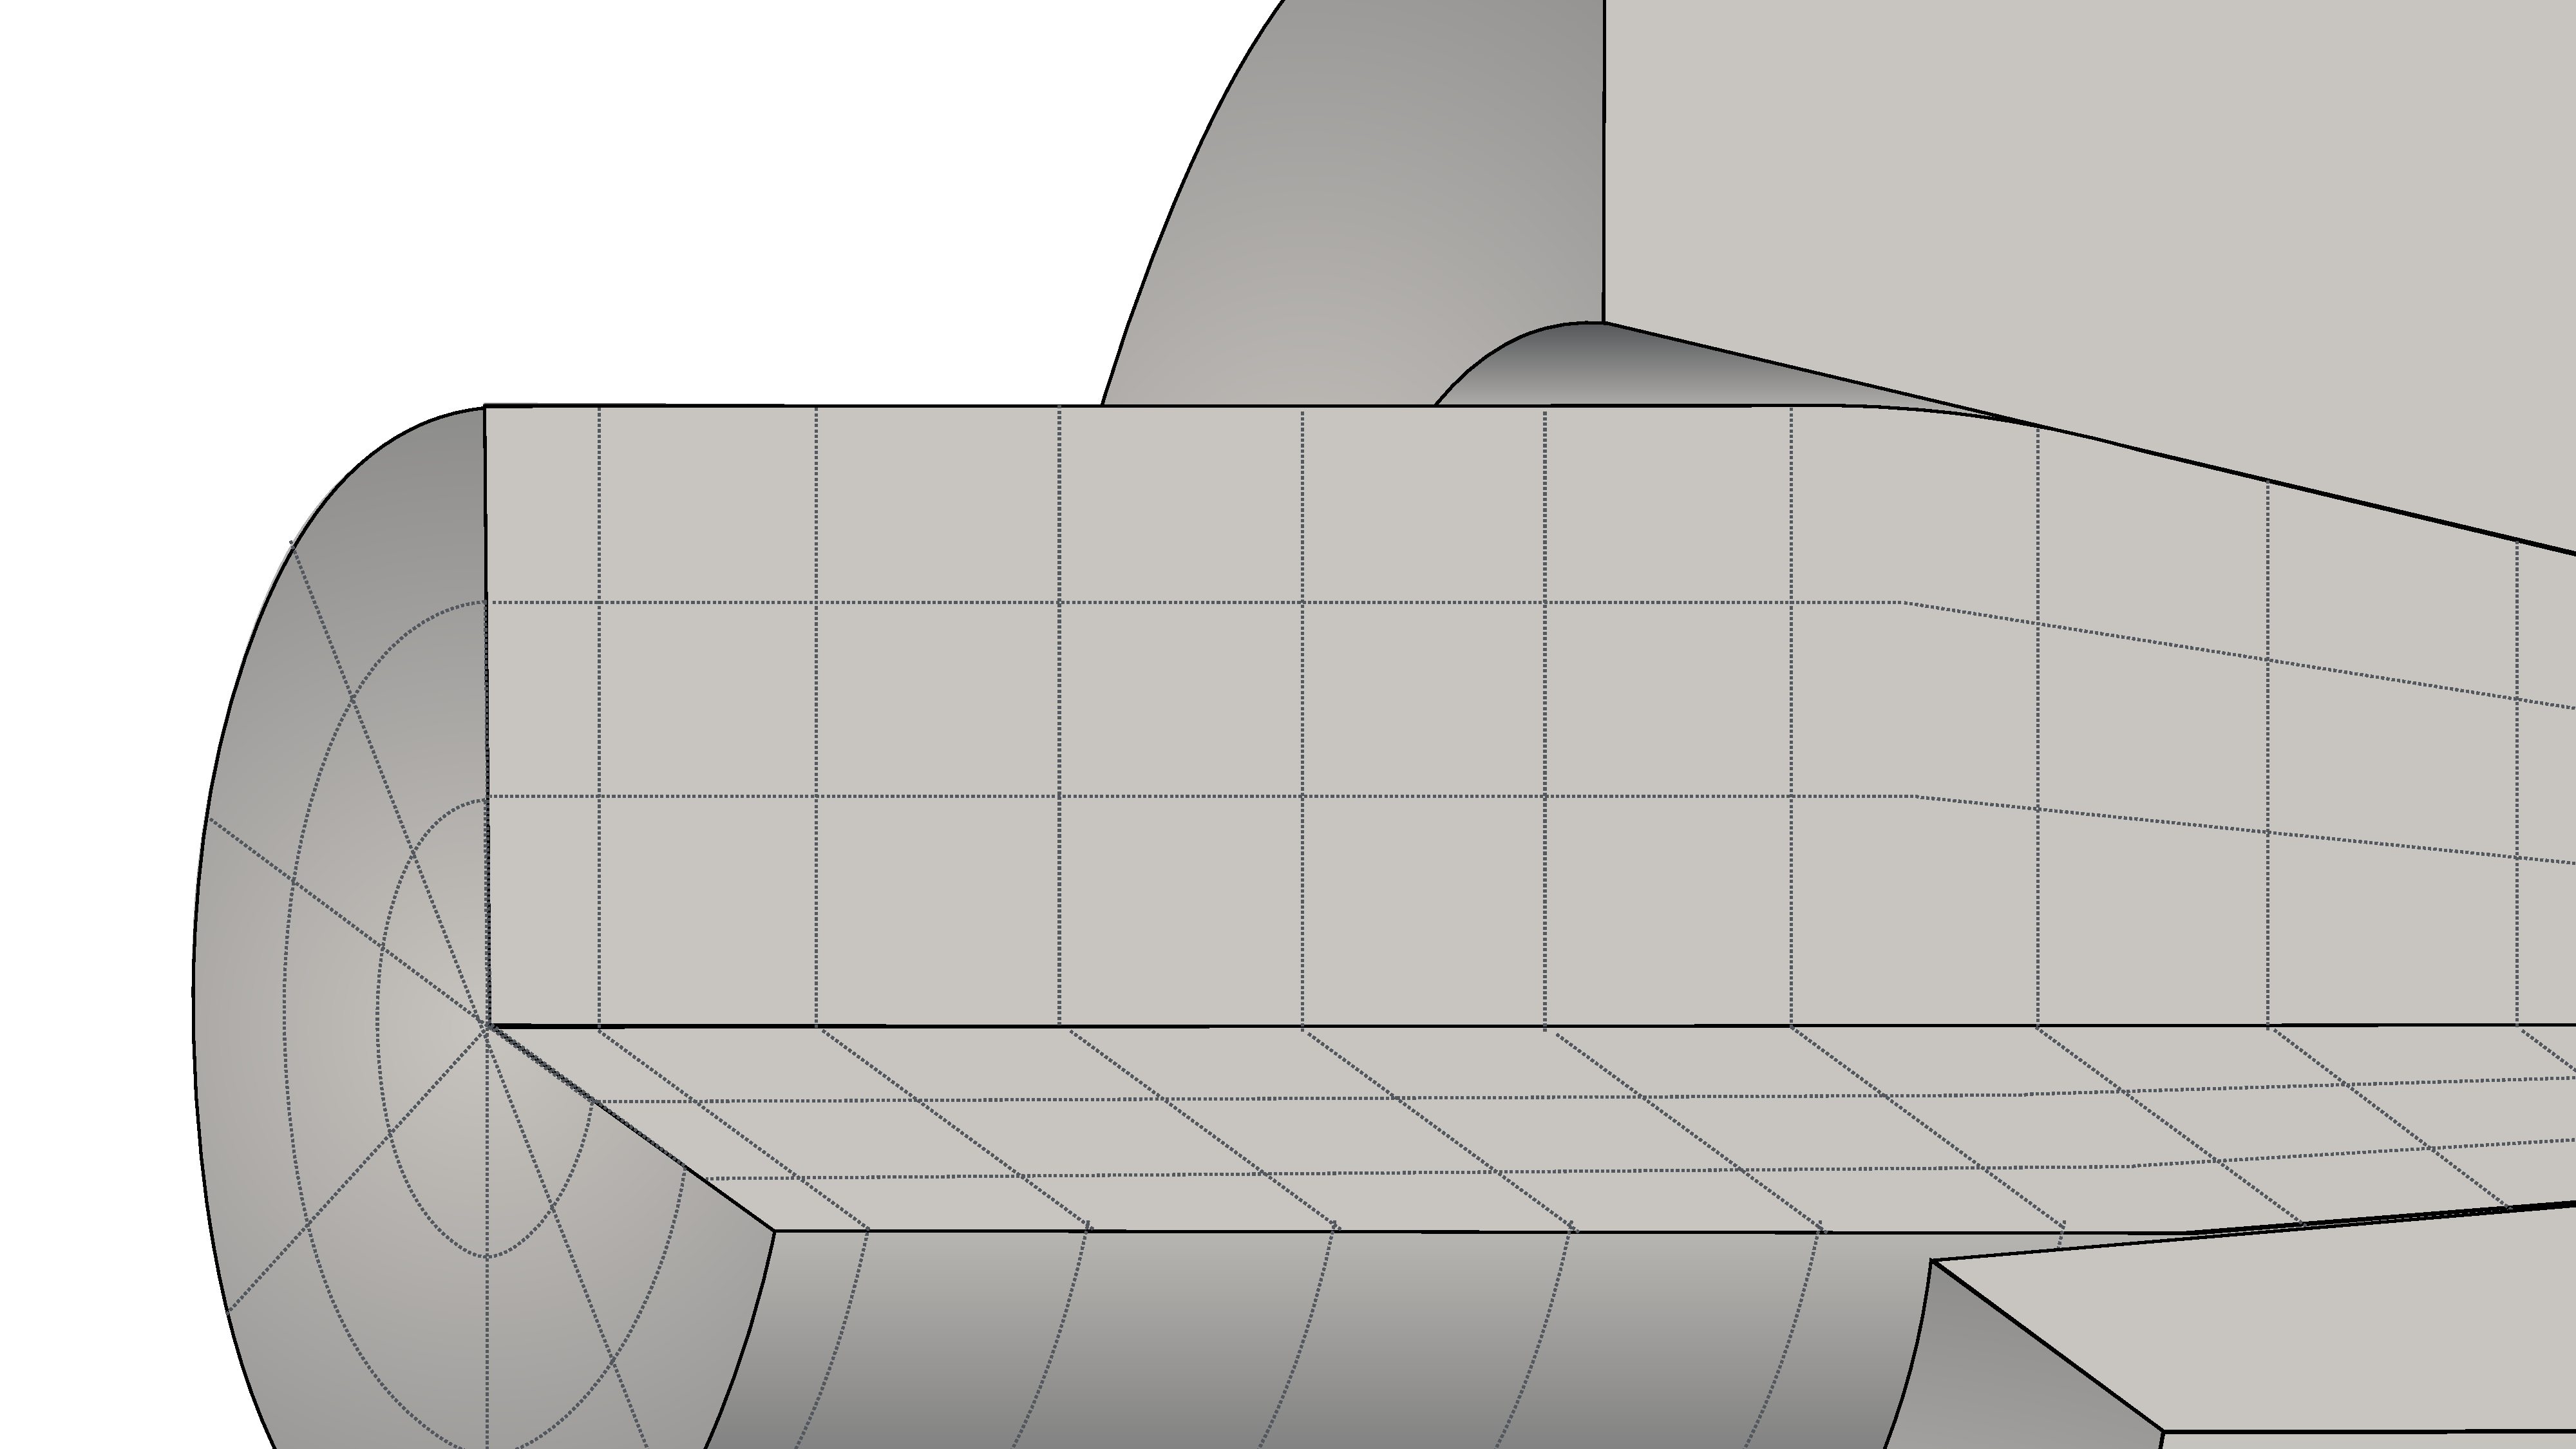
\includegraphics[width=0.3\textwidth]{./Figures/layerAddition/fig7}}
	\subfigure[] {\label{airbus}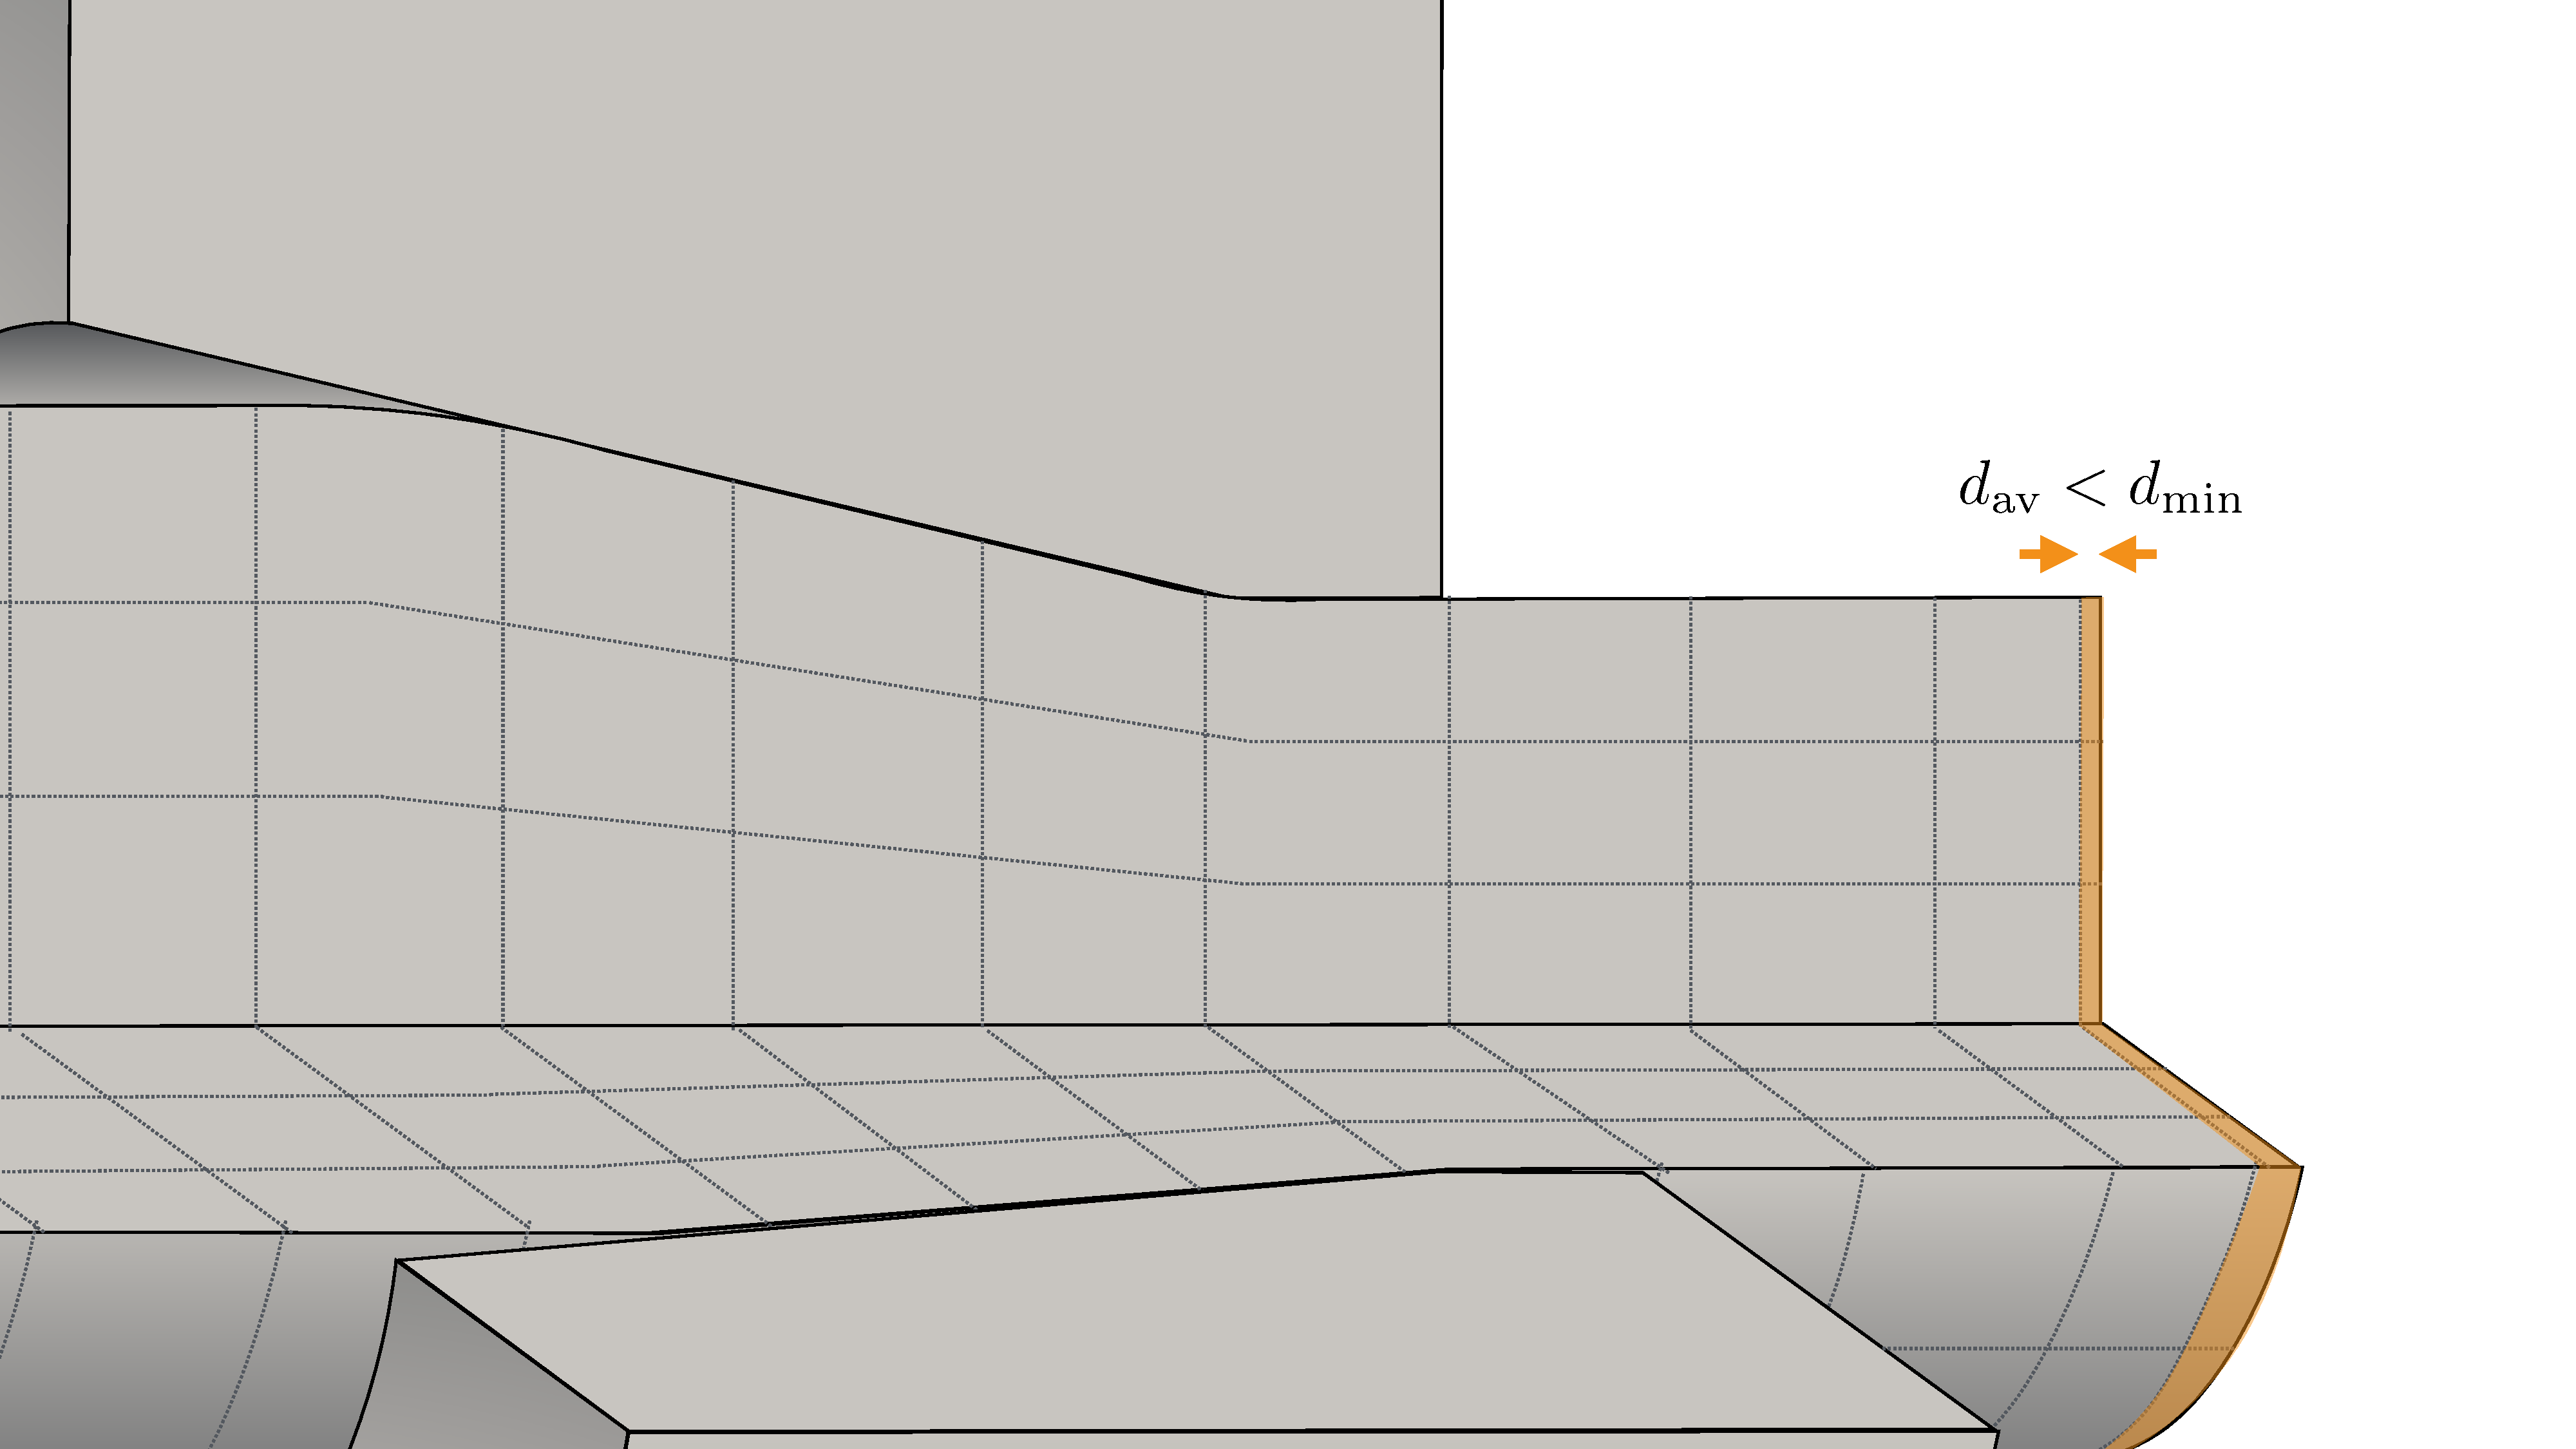
\includegraphics[width=0.3\textwidth]{./Figures/layerAddition/fig8}}
	\subfigure[] {\label{airbus}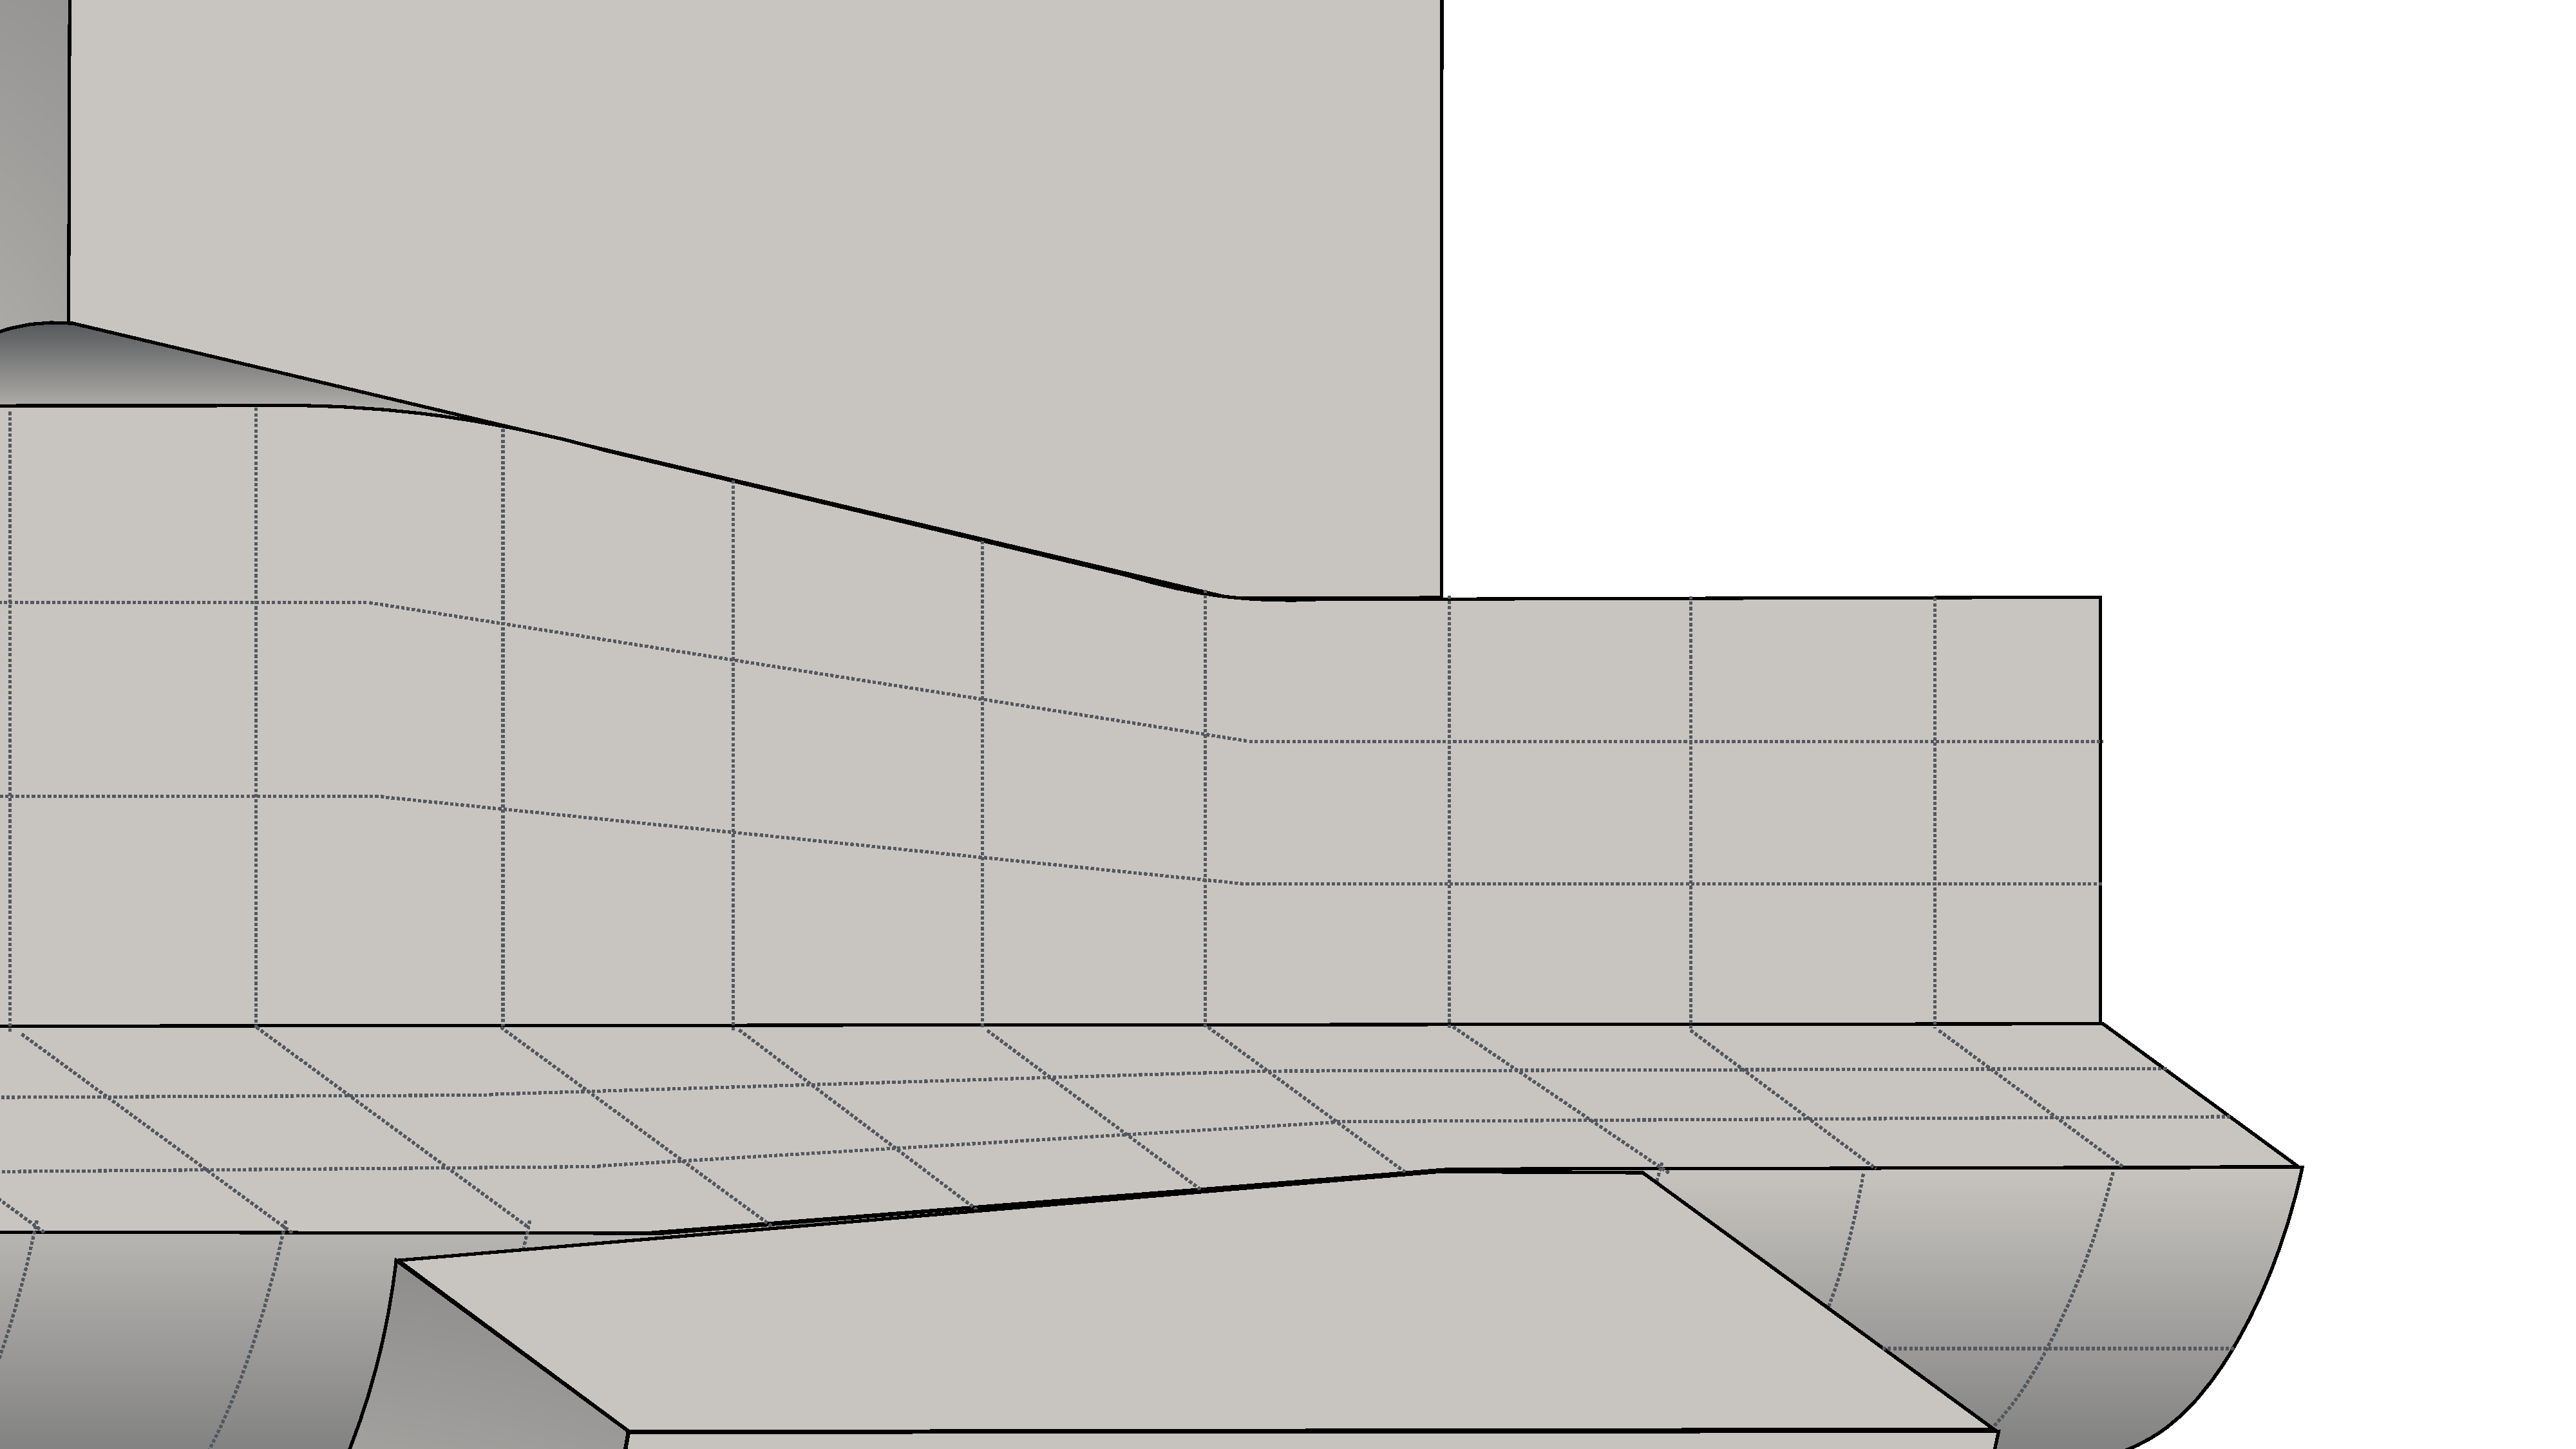
\includegraphics[width=0.3\textwidth]{./Figures/layerAddition/fig9}}
	\caption{Layer addition and removal mesh motion algorithm}
	\label{fig:layerAddition}
\end{figure}

Following the layer addition and removal mesh motion algorithm, solution and derived field data at the newly added cell centres are mapped from the field data stored at the upstream boundary.
This mapping approach assumes field data to have a zero gradient in the upstream direction; this assumption is valid if the upstream and downstream are chosen sufficiently far from the \emph{active} deformation zone.

\textbf{Note on parallelisation}: The proposed solution algorithm has been implemented in the open-source toolbox OpenFOAM, where multi-CPU-core parallelisation on distributed memory systems is achieved through the domain decomposition approach.
To simplify the implementation of the non-trivial topological mesh changes (addition or removal of cells), domain decomposition approaches have been limited to decomposing the workpiece into streamwise columns of cells (Figure \ref{fig:layerAdditionParallel}).
In the current approach, modified forms of the METIS \cite{metis} and scotch \cite{scotch} approaches have been used to perform this decomposition.
\begin{figure}[tbh]
	\centering
	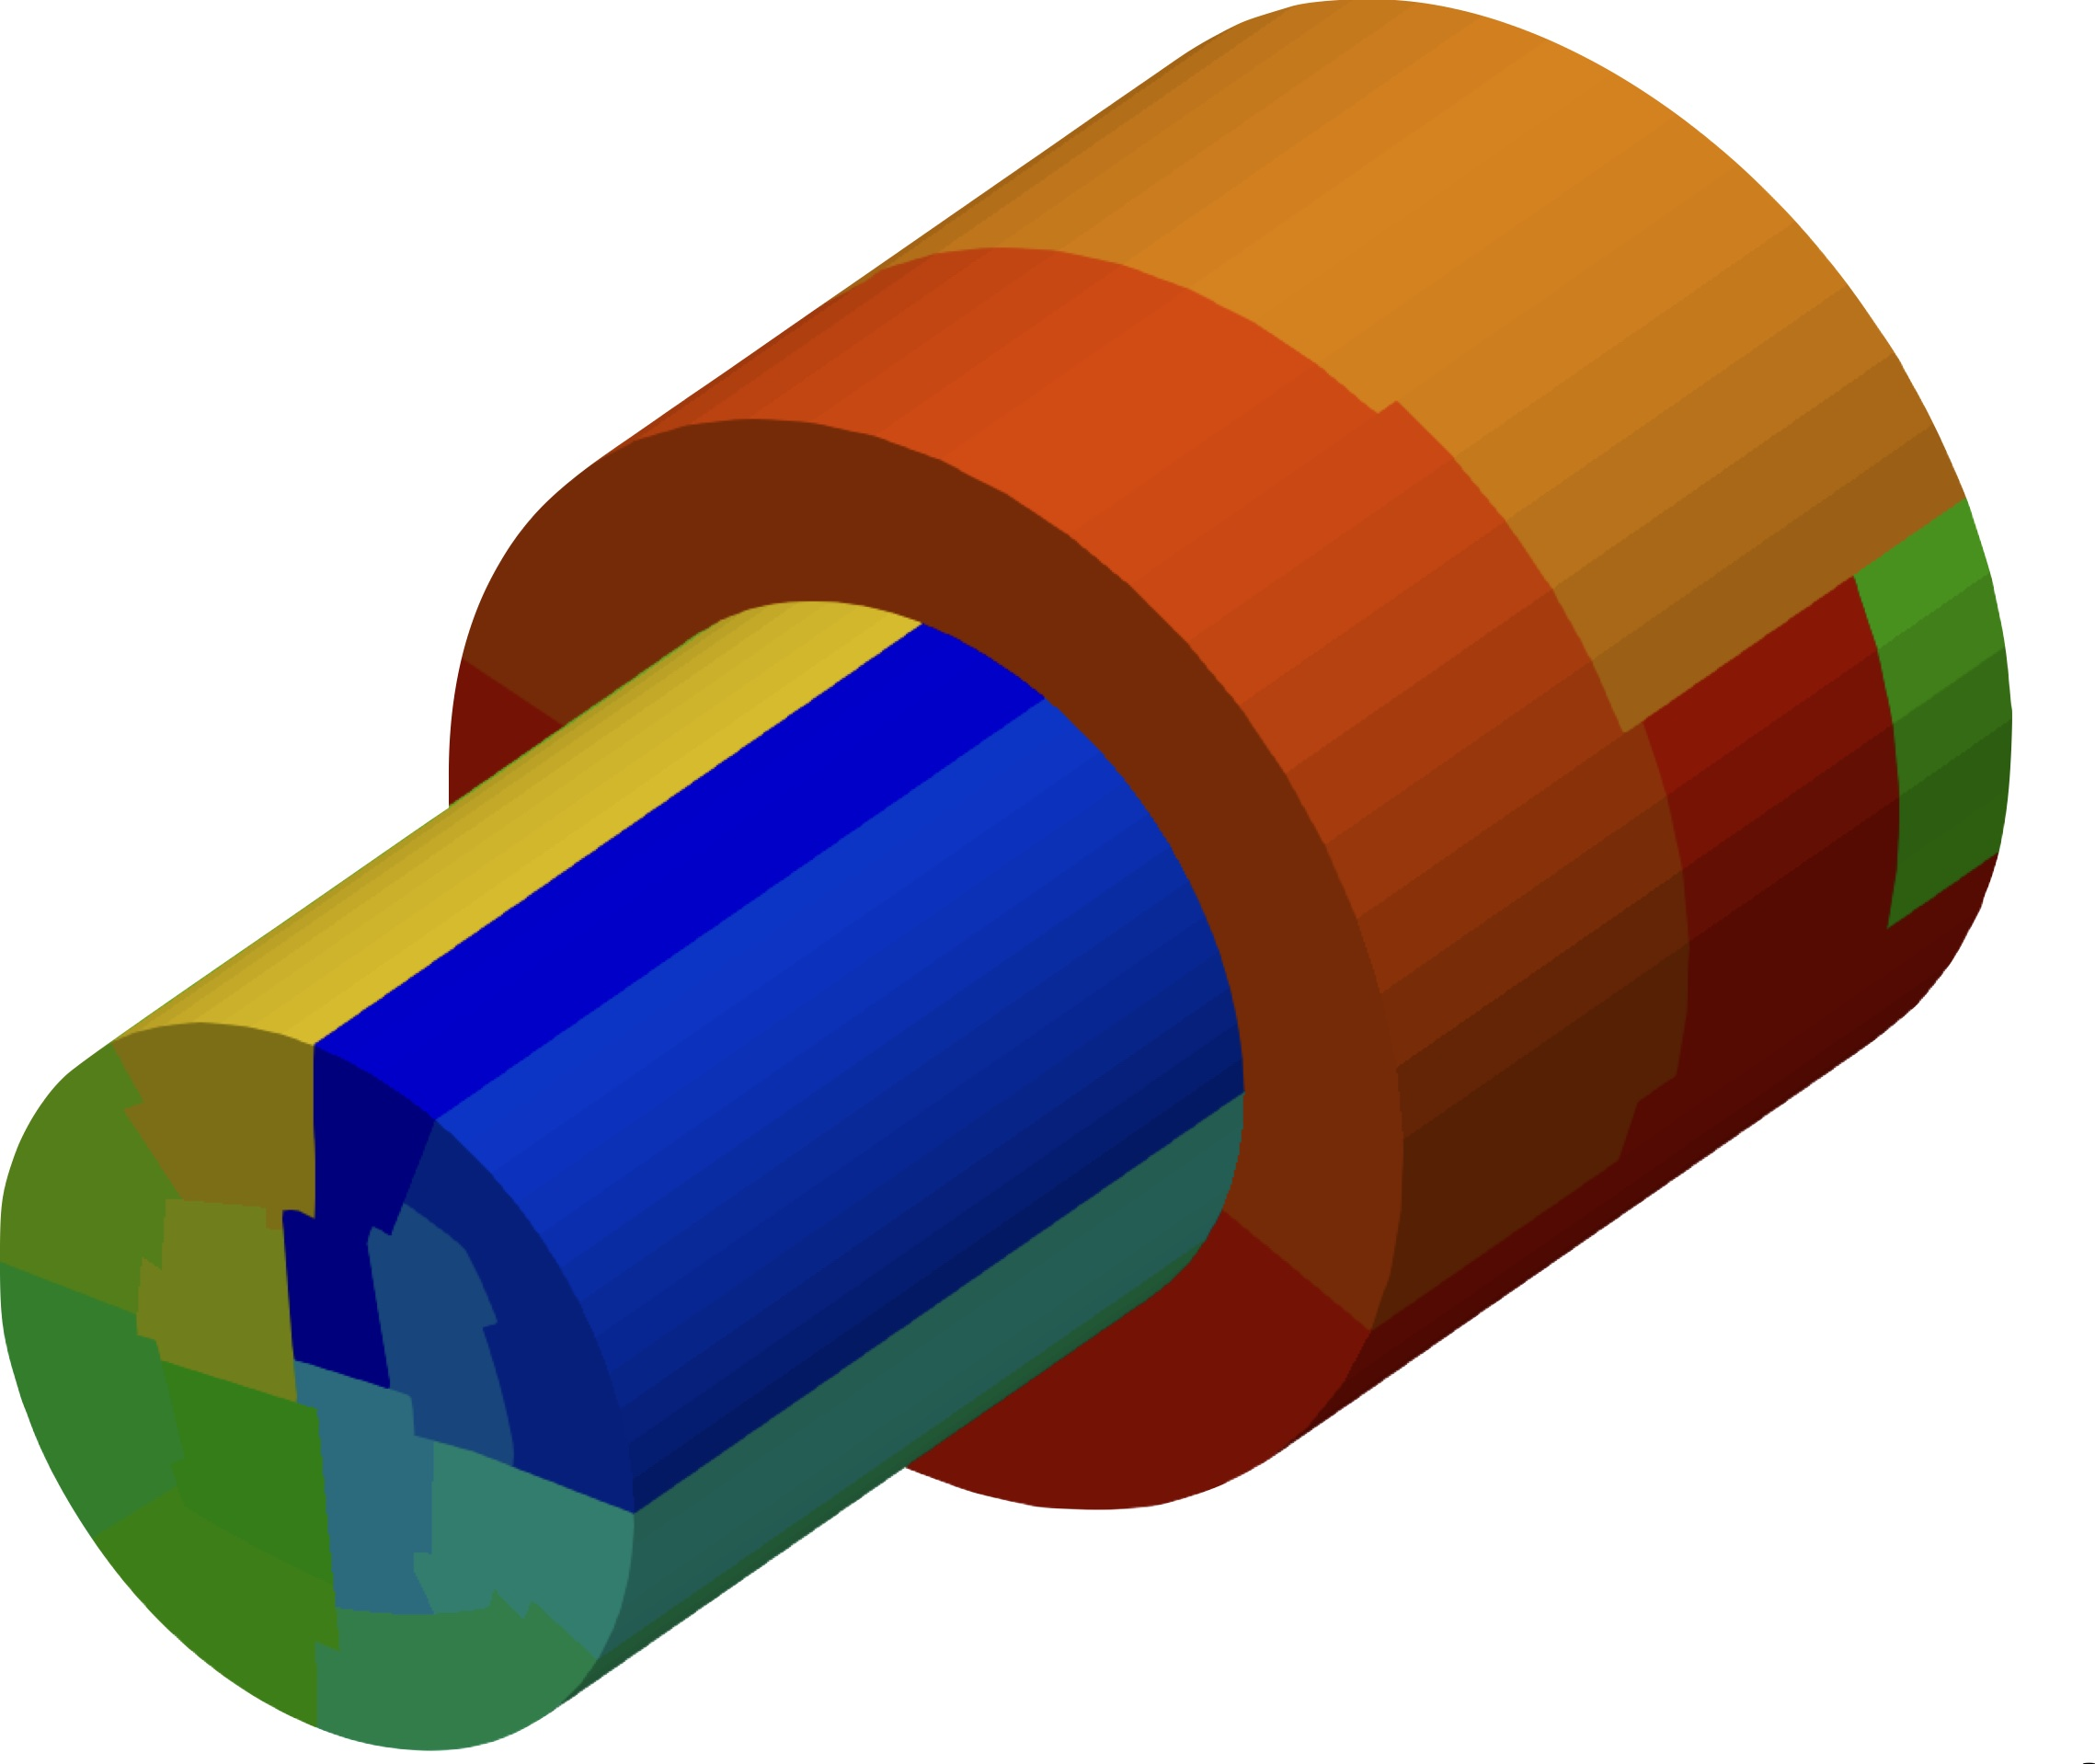
\includegraphics[width=0.45\textwidth]{./Figures/layerAddition/parallel}
	\caption{Example parallel decomposition of a wire and drawing die, where the wire is decomposed into streamwise \emph{columns}, indicated by the different colours. There is no limitation on the die decomposition.}
	\label{fig:layerAdditionParallel}
\end{figure}




%%%%%%%%%%%%%%%%%%%%%%%%%%%%%%%%%%%%%%%%%%%%%%%%%%%%%%%%%%%%%%%%%%
\section{Constitutive damage laws} \label{sec:constitutive_laws}
%%%%%%%%%%%%%%%%%%%%%%%%%%%%%%%%%%%%%%%%%%%%%%%%%%%%%%%%%%%%%%%%%%

%- maths details of the three damage laws
%- proposed modifications

\subsection{Overview}

As noted by \citet{garrison_ductile_1987}, ductile fracture in metals occurs in three stages: (i) voids are nucleated at material defects (usually inclusions), adding to pre-existing voids, if any; (ii) plastic deformations cause these voids to grow; and (iii) when large enough, these voids coalesce to form micro-cracks and macro-cracks.
Recent reviews of 
Approaches to model ductile fracture in metal forming can classified into two approaches \citep{cao_models_2017, tekkaya_damage_2020}: continuum damage mechanics models and micro-mechanical models.

In \emph{continuum} damage mechanics, an internal damage variable is used to describe the accumulation of microstructural degradation within a material due to various types of loading.
This degradation is typically reflected in the increased density of internal defects, such as microcracks, dislocations, or voids.
The internal damage variable is continuous, meaning it can take on any value within a given range.
The \emph{micro-mechanical} approach is also continuous in nature and posits the existence of material micro-voids.
The void density is described by a variable denoted as porosity.
Material degradation is characterised by increased porosity due to void nucleation, growth, and coalescence.
As noted by \citet{besson_continuum_2010, cao_models_2017} and \citet{tekkaya_damage_2020}, the canonical frameworks in the continuum damage mechanics and micro-mechanical approaches are the Lemaitre \cite{lemaitre_continuous_1985,lemaitre_engineering_2005} and the Gurson-Tvergaard-Needleman (GTN) \cite{gurson_continuum_1977,tvergaard_analysis_1984} models, respectively.

This section provides an overview of the classic Lemaitre and GTN models and proposes modifications to the Lemaitre model to extend its applicability to high hydrostatic pressure regimes characteristic of wire drawing.
For comparison, a recent phase field model damage approach is also considered.

The constitutive damage laws described in this section close the system of governing equations (Equation \ref{eqn:MomentumImplicitExplicit}) described in Section \ref{sec:solDomDiscret}, by providing the definition of stress.

%In this chapter, a brief description of the historical development of these models will be provided, and suitable algorithmic implementations of them will be developed and described. More recent developments in the formulations of these models are also described and implemented. 

%\begin{figure}[htb]
%\begin{center}
%	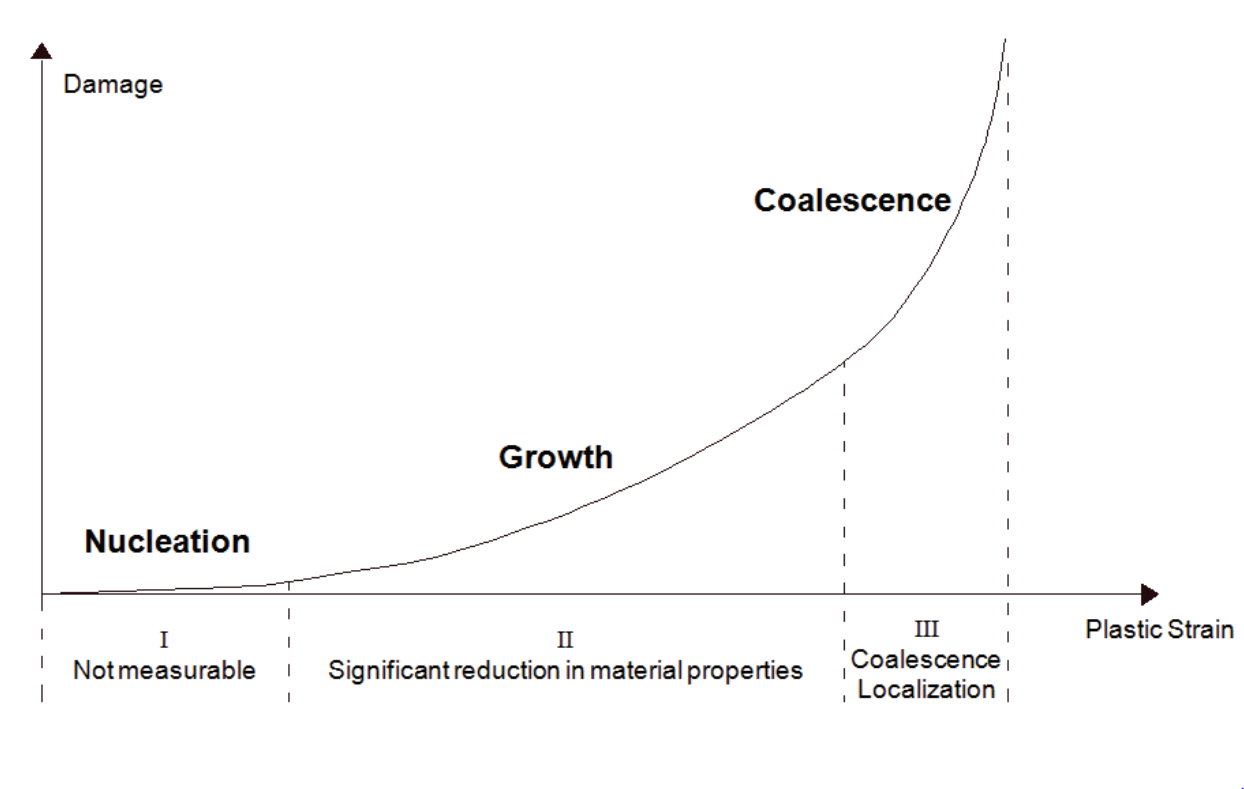
\includegraphics[width=0.65\textwidth]{./Figures/damageModels/ductileDamageEvolution.png}
%\caption{Ductile damage evolution \cite{teixeira_ductile_2010}}
%\label{fig:Ductile-damage-evolution}
%\end{center}
%\end{figure}
%
%\begin{figure}[htb]
%\begin{center}
%	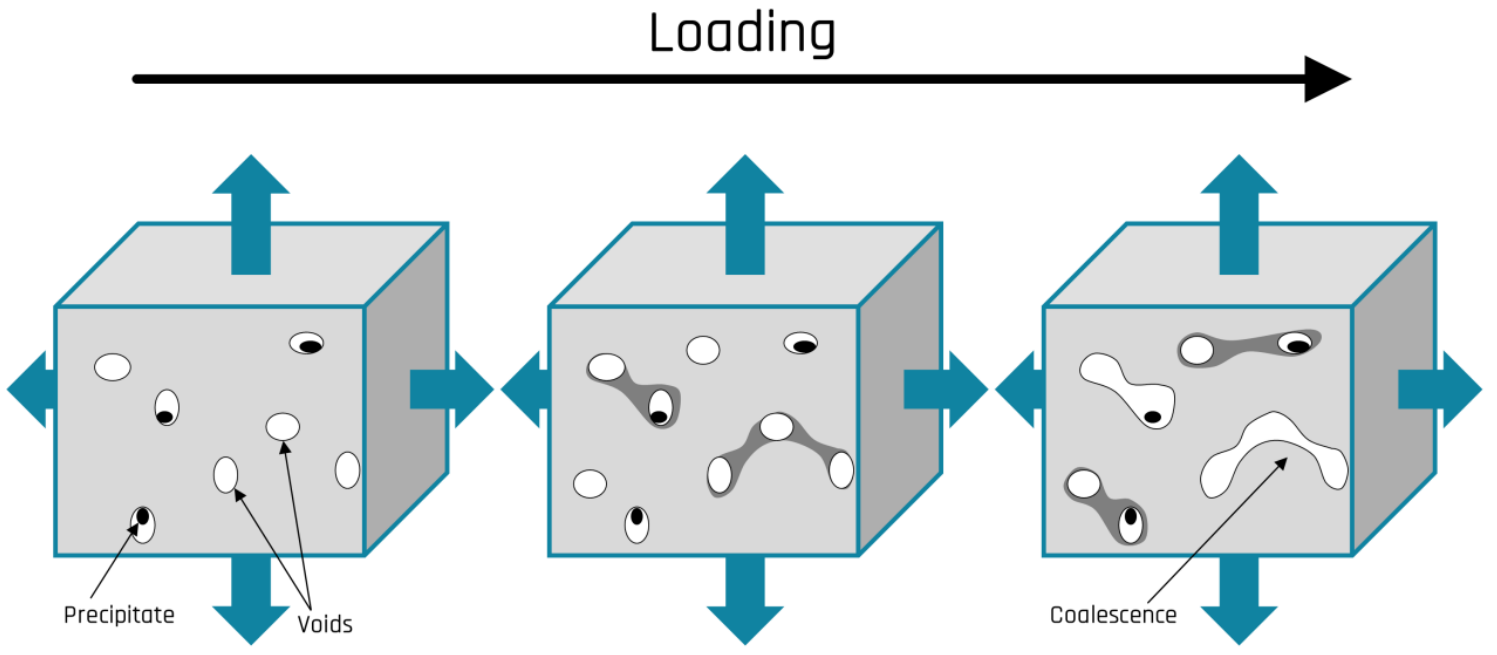
\includegraphics[width=0.65\textwidth]{./Figures/damageModels/f_ngc.png}
%\caption{Illustration of the nucleation, growth and coalescence of voids \cite{archie_damage_2018}}
%\label{fig:Nucleating Voids}
%\end{center}
%\end{figure}

\subsection{Preliminaries}
Before describing these models in more detail, it is necessary to define the stress triaxiality $\eta$ and the Lode angle $\theta$ and related Lode parameters \cite{bai_new_2008, nahshon_modification_2008}.
Extensive literature has noted the importance of stress triaxiality and Lode angle in predicting ductile fracture \cite{besson_continuum_2010,cao_models_2017,tekkaya_damage_2020}.
The triaxiality parameter $\eta$ is given by:
\begin{equation} % note: different pressure convention from Andrew's thesis
    \eta = -\frac{p}{\sigma_{v}}
\end{equation}
where, as noted previously, $p = -\text{tr}(\boldsymbol{\sigma})/3$ is the hydrostatic pressure, and $\sigma_{v} = \sqrt{3 J_2} = \sqrt{\frac{3}{2} \text{dev}(\bb{\sigma}) : \text{dev}(\bb{\sigma}) }$ is the equivalent (von Mises) stress.
$J_2$ is the second invariant of the deviatoric stress tensor.
%The trace operator is indicated by $\text{tr}(\bullet)$,
The deviatoric operator is indicated by $\text{dev}(\bullet)$, and $:$ indicates the double-dot product.

The Lode angle $0 \leq \theta \leq \frac{\pi}{3}$ physical interpretation relates to the degree of shear dominance present in the stress state.
It can be rewritten as a function of the normalised third invariant of the deviatoric stress tensor:
\begin{equation}
    \theta=\frac{1}{3} \arccos\left(\xi\right)
\end{equation}

The parameter $0 \leq \xi \leq 1$ is determined as a ratio between the third invariant and the equivalent stress:
\begin{equation}
	\xi = \left(\frac{r}{\sigma_{v}}\right)^3
\end{equation}
where $r$ is given by:
\begin{equation}
	r  = 3 \left(\frac{3}{2}J_3\right)^{1/3} %= 3 \left(\frac{3}{2}\text{det}\left(\mathbf{s}\right)\right)^{1/3}	
\end{equation}
The third invariant of the deviatoric stress tensor is $J_3 = \text{det}[\text{dev}(\mathbf{s})]$.
% $\mathbf{s}
%The Lode angle ranges between $0$ and $\frac{\pi}{3}$.
%The range of $\xi$ is between $-1$ and $1$.
An alternative normalised Lode angle has been proposed by \citet{bai_new_2008} to be
\begin{equation}
	\bar{\theta}=1-\frac{6\theta}{\pi}	
\end{equation}
which ranges between -1 and 1.

The three Lode parameters ($\theta$, $\xi$, and $\bar{\theta}$) are essentially equivalent but are defined to vary between different limits.


\subsection{Isotropic Elastoplasticity}

%\hl{Introduce the Kirchhoff stress tau and dot gamma and spatially rotated plastic stretch and thermodynamic force chi (x) and elastic rotation tensor}

\subsubsection{Model Formulation}

In the current work, the damage models are formulated in terms of isotropic $J_2$ (von Mises) elastoplasticity.
Extension to other forms of elastoplasticity (e.g., kinematic hardening, anisotropic/Hill yielding, distortional hardening) is possible but is outside the scope of this article.
The adopted large strain elastoplasticity formulation is based on the logarithmic (Hencky) strain, as proposed by \citet{eterovic_hyperelastic-based_1990} and described in detail by \citet{koji_inelastic_2010} and \citet{de_souza_neto_computational_2008}.
This approach allows an additive split of the elastic and plastic strain tensors, conveniently leading to a return mapping scheme that is similar in form to those used in small-strain deformation models.
%To this author's eye, this is a formulation for elastoplasticity that is more lucid and relatively simple to implement in codes in comparison to the approach of \citet{simo_computational_1998}, for example.
%With an eye for future works, there also exists a well-established approach to extending large-strain elastoplasticity using the logarithmic strain to incorporate anisotropic and kinematic plasticity \cite{papadopoulos_formulation_2001,mettler_numerical_2012}.
In contrast, previous large-strain elastoplastic models \citep{cardiff_lagrangian_2017, clancy_improving_2019} implemented in the OpenFOAM software have adopted the approaches of \citet{caminero_modeling_2011} and \citet{simo_computational_1998}.
% and  this work represents, to the author's knowledge, the first time that the formulation by \citet{eterovic_hyperelastic-based_1990} for elastoplasticity has been implemented in OpenFOAM.


%First a dissipation potential $F$ is defined:
%\begin{equation}
%    F=F_p
%\end{equation}
%Where $F_{p}$ is the dissipation associated with the plasticity. Given the assumption of plastic isotropy and applying the generalized normality rule:
%\begin{equation}
%    \bar{\mathbf{d}}^p=\dot{\gamma}\frac{\partial F}{\partial\boldsymbol{\tau}}
%\end{equation}
%And
%\begin{equation}
%    \dot{\alpha}=-\dot{\gamma}\frac{\partial F}{\partial\chi}
%\end{equation}
%Equation 3.30 can be defined in terms of the multiplicative plastic deformation gradient $\mathbf{F}^{p}$ by combining it with equation \ref{eqn:rotatedPlasticStretch} to give
%\begin{equation}
%    \dot{\mathbf{F}^p\mathbf{F}^{p-1}}=\dot{\gamma}\mathbf{R}^{eT}\frac{\partial F}{\partial\boldsymbol{\tau}}\mathbf{R}^e
%\end{equation}

The employed isotropic $J_2$ elastoplastic constitutive law is defined in terms of the yield criterion
\begin{eqnarray} \label{eq:yieldFunc}
	%    F_p &=& \tau_{eq} - \sigma_y\left(\alpha\right) \\
	\Phi &=& \sigma_v \; - \; \sigma_y\left(\bar{\varepsilon}_p \right)
\end{eqnarray}
%\end{equation}
%Where $\tau_{eq}$ is the von Mises equivalent stress:
%\begin{equation}
%    \tau_{eq} = \sqrt{\frac{3}{2}\boldsymbol{\tau}_d:\boldsymbol{\tau}_d}
%\end{equation}
%Multivariable calculus operations are used to obtain the following constitutive equations
%\begin{equation}
and flow rule
\begin{eqnarray} \label{eq:flowRule}
    %\frac{\partial}{\partial t} \left(\mathbf{F}_p \mathbf{F}_p^{-1} \right)
    \dot{\mathbf{F}}_p \cdot \mathbf{F}_p^{-1}
    &=&
	%    \dot{\gamma}\mathbf{R}^{eT}\left(\frac{3}{2}\frac{\boldsymbol{\tau}_d}{\tau_{eq}}\right)\mathbf{R}^e
    \dot{\bar{\varepsilon}}_p \; \mathbf{R}_e^T \cdot 
    \left[
    \frac{3}{2} \frac{\text{dev}\left(\boldsymbol{\sigma} \right)} {\sigma_{v}}
    \right]
    \cdot  \mathbf{R}_e
\end{eqnarray}
where the yield stress $\sigma_y$ is a function of the hardening variable $\bar{\varepsilon}_p$ coincides with the equivalent plastic strain $\bar{\varepsilon}_p$.
The deformation gradient is decomposed into elastic and plastic components $\bb{F} = \bb{F}_e \cdot \bb{F}_p$ and polar decomposition of the elastic deformation gradient gives the elastic rotation $\bb{R}_e$ and elastic stretch $\bb{U}_e$ tensors: $\bb{F}_e = \bb{R}_e \cdot \bb{U}_p$.

%\begin{equation}
%\dot{\alpha}=\dot{\gamma}
%\end{equation}
%It's worth noting that the hardening variable $a$ used in this model is the equivalent plastic strain which can be given by $\bar{\varepsilon}^p$.
The model is closed with the Kuhn-Tucker conditions
\begin{eqnarray}
	\Phi \geq 0, \quad\quad
	\dot{\bar{\varepsilon}}_p \geq 0, \quad\quad
	\dot{\bar{\varepsilon}}_p \Phi = 0
\end{eqnarray}
and the consistency condition
\begin{eqnarray}
	\dot{\bar{\varepsilon}}_p \dot{\Phi} &=& 0
\end{eqnarray}


\subsubsection{Computational procedure}
%For a displacement-based finite volume procedure, the discretised equilibrium equations are solved for each time step using an iterative method to achieve convergence. The displacement field is solved at each iteration using the stress field calculated from the elasto-plastic return mapping scheme. This displacement field is then used to find a new value for the stress from the elasto-plastic return mapping scheme. This iterative procedure continues until convergence is achieved.

For each cell at every outer (Picard) iteration, the stress $\bb{\sigma}^{[m+1]}$ and history variables ($\alpha^{[m+1]}$, $\bb{F}_p^{[m+1]}$) at time step $t^{[m+1]}$ must be calculated in terms of the current displacement increment gradient $[\bb{\nabla} (\Delta \bb{u})]^{[m+1]}$ and old-time history variables ($\alpha^{[m]}$, $\bb{F}_p^{[m]}$).

%the incremental displacement field $\Delta \mathbf{u}$ for the current time step $t^{[m+1]}$, at the current (outer) iteration, is provided. The values of the following variables are given from the previous time step:
%\begin{equation}
%    \left\{\mathbf{F}_n^p,\ \alpha_n\right\}
%\end{equation}
%The goal is then to have an algorithm to obtain the following variables at time $t^{[m+1]}$
%\begin{equation}
%    \left\{\mathbf{F}^{[m+1]}^p,\ \alpha^{[m+1]},\boldsymbol{\sigma}^{[m+1]}\right\}
%\end{equation}
%In order to obtain these values, the algorithm must satisfy the set of constitutive equations:
%\begin{equation}
%\left\{\begin{array}{c}
%    \dot{\mathbf{F}^p\mathbf{F}^{p-1}}=\dot{\gamma}\mathbf{R}^{eT}\left(\frac{3}{2}\frac{\boldsymbol{\tau}_d}{\tau_{eq}}\right)\mathbf{R}^e \\
%\dot{\alpha}=\dot{\gamma}
%\end{array}\right.
%\end{equation}

%To begin, equation 3.35 is integrated using the one-step implicit integration operator corresponding to the Euler backward method \cite{andrade_ductile_2011} to get:
%\begin{equation}
%    \mathbf{F}^{[m+1]}^p=exp\left[\frac{3}{2}\Delta\gamma\mathbf{R}^{[m+1]}^{e^T}\frac{{\bb{\tau}}_{d^{[m+1]}}}{\tau^{eq}^{[m+1]}}
%    \mathbf{R}^{[m+1]}^e\right]\mathbf{F}_n^p
%\end{equation}
%Due to plastic isotropy, this equation can be written as:
%\begin{equation}
%    \mathbf{F}^{[m+1]}^p=\mathbf{R}^{[m+1]}^{e^T}exp\left[\frac{3}{2}\Delta\gamma\frac{{\boldsymbol{\tau}_d}^{[m+1]}}{\tau^{eq}^{[m+1]}}\right]\mathbf{R}^{[m+1]}^e\mathbf{F}_n^p
%\end{equation}
%This represents the update of the plastic deformation gradient. This can in turn be combined with the fact that $\mathbf{F}=\mathbf{F}^{e}\mathbf{F}^{p}$ to give the elastic deformation tensor:
%\begin{equation}
%    \mathbf{F}^{[m+1]}^e={\mathbf{F}^{[m+1]}^{e\ trial}\mathbf{R}}^{[m+1]}^{e^T}exp\left[-\frac{3}{2}\Delta\gamma\frac{{\boldsymbol{\tau}_d}^{[m+1]}}{\tau^{eq}^{[m+1]}}\right]\mathbf{R}^{[m+1]}^e
%\end{equation}
%where $\mathbf{F}^{[m+1]}^{e\ trial}$ is given by:
%\begin{equation}
%\mathbf{F}^{[m+1]}^{e\ trial}=\mathbf{f}^{[m+1]}\mathbf{F}^{[m+1]}^{e}
%\end{equation}
%$\mathbf{f}^{[m+1]}$ is the relative deformation gradient (equation 2.45). 
%Using the fact that $\mathbf{F}^e=\mathbf{V}^{e}\mathbf{R}^{e}$
%\begin{equation}
%    \mathbf{V}^{[m+1]}^e\mathbf{R}^{[m+1]}^e={\mathbf{F}^{[m+1]}^{e\ trial}\mathbf{R}}^{[m+1]}^{e^T}exp\left[-\frac{3}{2}\Delta\gamma\frac{{\boldsymbol{\tau}_d}^{[m+1]}}{\tau^{eq}^{[m+1]}}\right]\mathbf{R}^{[m+1]}^e
%\end{equation}
%Multiplying both sides by $\mathbf{R}^{e^T}^{[m+1]}$
%\begin{equation}
%    \mathbf{V}^{[m+1]}^e={\mathbf{F}^{[m+1]}^{e\ trial}\mathbf{R}}^{[m+1]}^{e^T}exp\left[-\frac{3}{2}\Delta\gamma\frac{{\boldsymbol{\tau}_d}^{[m+1]}}{\tau^{eq}^{[m+1]}}\right]
%\end{equation}
%Multiplying by the inversion of the exponential term:
%\begin{equation}
%    \mathbf{V}^{[m+1]}^{e}exp\left[\frac{3}{2}\Delta\gamma\frac{{\boldsymbol{\tau}_d}^{[m+1]}}{\tau^{eq}^{[m+1]}}\right]={\mathbf{F}^{[m+1]}^{e\ trial}\mathbf{R}}^{[m+1]}^{e^T}
%\end{equation}
%Taking the square of both sides:
%\begin{equation}
%    \mathbf{V}^{[m+1]}^{e}\ exp\left[3\Delta\gamma\frac{{\boldsymbol{\tau}_d}^{[m+1]}}{\tau^{eq}^{[m+1]}}\right]\mathbf{V}^{[m+1]}^{e}={\mathbf{F}^{[m+1]}^{e\ trial}\mathbf{R}}^{[m+1]}^{e^T}{\mathbf{F}^{[m+1]}^{{e\ trial}^T}\mathbf{R}}^{[m+1]}^{e}
%\end{equation}
%
%Isolating the RHS of this equation and using the fact that $\mathbf{R}^{e^T}^{[m+1]}\mathbf{R}^{e}^{[m+1]}=\textbf{I}$:
%\begin{equation}
%    {\mathbf{F}^{[m+1]}^{e\ trial}\mathbf{R}}^{[m+1]}^{e^T}{\mathbf{F}_{\mathbf{n}+1}^{{e\ trial}^T}\mathbf{R}}^{[m+1]}^e=\mathbf{F}^{[m+1]}^{e\ trial}\mathbf{F}^{[m+1]}^{{e\ trial}^T}=\left(\mathbf{V}^{[m+1]}^{e\ trial}\right)^\mathbf{2}
%\end{equation}
%
%Subbing this into equation 3.47 we get:
%\begin{equation}
%    \mathbf{V}^{[m+1]}^e exp\left[3\Delta\gamma\frac{{\boldsymbol{\tau}_d}^{[m+1]}}{\tau^{eq}^{[m+1]}}\right]\mathbf{V}^{[m+1]}^e=\left(\mathbf{V}^{[m+1]}^{e\ trial}\right)^\mathbf{2}
%\end{equation}
%
%By rearranging and taking the square root of both sides, the following can be obtained:
%\begin{equation}
%    \mathbf{V}^{[m+1]}^e=\mathbf{V}^{[m+1]}^{e\ trial}exp\left[-\frac{3}{2}\Delta\gamma\frac{{\boldsymbol{\tau}_d}^{[m+1]}}{\tau^{eq}^{[m+1]}}\right]
%\end{equation}
%
%Taking the natural log of both sides:
%\begin{equation}
%    ln\left(\mathbf{V}^{[m+1]}^{e}\right)=ln\left(\mathbf{V}^{[m+1]}^{e\ trial}exp\left[-\frac{3}{2}\Delta\gamma\frac{{\boldsymbol{\tau}_d}^{[m+1]}}{\tau^{eq}^{[m+1]}}\right]\right)
%\end{equation}
%
%Using the fact that $ln\textbf{V}=\boldsymbol{\varepsilon^e}$ (equation 3.8), the additive split of the elastic and plastic strain tensors is derived:
%\begin{equation}
%    \boldsymbol{\varepsilon}^{[m+1]}^{e}=\boldsymbol{\varepsilon}^{[m+1]}^{e\ trial}-\frac{3}{2}\Delta\gamma\frac{{\boldsymbol{\tau}_d}^{[m+1]}}{\tau^{eq}^{[m+1]}}
%\end{equation}
%The integration of the other constitutive equations using the backwards Euler scheme is simply given by:
%\begin{eqnarray}
%    \alpha^{[m+1]}-\alpha_n=\Delta\gamma  \notag \\
%    \alpha^{[m+1]}=\alpha_n+\Delta\gamma  
%\end{eqnarray}
%The final system of equations to be solved when the material is on the plastic domain is given by:
%\begin{equation}
%	\left\{\begin{array}{c}
%	\label{eqn:dicritisedFinalEquationsPLasticity}
%	F_p = \tau^{eq}^{[m+1]} - \sigma_{y} \left(\alpha^{[m+1]}\right)=0 \\
%	\boldsymbol{\varepsilon}^{[m+1]}^e = \boldsymbol{\varepsilon}^{[m+1]}^{e\ trial}
%		- \frac{3}{2} \Delta \gamma \frac{{\boldsymbol{\tau}_d}^{[m+1]}}{\tau^{eq}^{[m+1]}} \\
%		\alpha^{[m+1]}=\alpha_n+\Delta \gamma
%	\end{array}\right.
%\end{equation}
%The above system of equations can be resolved by solving for the plastic increment using an implicit algorithm. It can be shown that the equations in \ref{eqn:dicritisedFinalEquationsPLasticity} can be satisfied by solving the yield equation for the plastic increment $\Delta \gamma$. To begin, the von Mises yield criterion is restated:
%\begin{equation}
%    \tau^{eq}^{[m+1]}-\sigma_y\left(\alpha^{[m+1]}\right)=0
%\end{equation}
%
%Recalling the definition of the von Mises stress (equation 3.34), the equivalent stress can be expressed in terms of the elastic strain and combined with equation 3.53 to give:
%\begin{eqnarray}
%\tau^{eq}^{[m+1]}&=&\sqrt{\frac{3}{2}}\left\|2 \mu \operatorname{dev}\left(\boldsymbol{\varepsilon}^{[m+1]}^e\right)\right\| \\ \notag
%&=&
%\sqrt{\frac{3}{2}}\left\|2 \mu \operatorname{dev}\left(\boldsymbol{\varepsilon}^{[m+1]}^{e \text { trial }}-\frac{3}{2}\Delta \gamma\frac{{\boldsymbol{\tau}_d}^{[m+1]}}{\tau^{eq}^{[m+1]}}\right)\right\|
%\end{eqnarray}
%
%Given that:
%\begin{equation}
%\left\|2 \mu \operatorname{dev}\left(\frac{3}{2} \Delta \gamma \frac{{\boldsymbol{\tau}_d}^{[m+1]}}{\tau^{eq}^{[m+1]}}\right)\right\|=3 \mu \Delta \gamma
%\end{equation}
%The von Mises equivalent stress can be expressed as:
%\begin{equation}
%\tau^{eq}^{[m+1]}=\sqrt{\frac{3}{2}}\left\|2 \mu \operatorname{dev}\left(\boldsymbol{\varepsilon}^{[m+1]}^{e \text { trial }}\right)\right\|-3 \mu \Delta \gamma
%\end{equation}
%The following relation for the equivalent stress can therefore be obtained:
%\begin{equation}
%	\tau^{eq}^{[m+1]}=\tau^{eq}_{{n+1}^{\text{trial}}} - 3 \mu \Delta \gamma
%\end{equation}
%Combining equation 3.60 with 3.56, the yield function can be given in terms of the plastic increment:
%\begin{equation}
%\tau^{eq}_{{n+1}^{\text {trial }}}-3 \mu \Delta \gamma-\sigma_y\left(\alpha_n+\Delta \gamma\right)=0
%\end{equation}
%This is solved implicitly using the Newton–Raphson method for $\Delta \gamma$ , the stress tensor and the plastic strain tensor are then updated based on this value.

The adopted stress calculation algorithm \citep{de_souza_neto_computational_2008} is summarised in Algorithm \ref{alg:stressAlg}.

\hl{Andrew: why is J not equal to det(F) in pressure calculation?}\\
\begin{algorithm}[htb] \label{alg:stressAlg}
\SetAlgoLined
(i) Update deformation gradients for a given incremental displacement

\begin{equation}
  \mathbf{f}^{[m+1]} = \mathbf{I} + \left[ \bb{\nabla}(\Delta\textbf{u}) \right]^T \nonumber
\end{equation}

\begin{equation}
  \mathbf{F}^{[m+1]} = \mathbf{f}^{[m+1]} \cdot \mathbf{F}^{[m]}  \nonumber
\end{equation}

(ii) Compute trial elastic state
\begin{equation}
\mathbf{B}_{e}^{[m]} = \exp\left({2\boldsymbol{\varepsilon}_{e}^{[m]}}\right) \nonumber
\end{equation}
\begin{equation}
\mathbf{B}_{e}^{\text{trial}} = \mathbf{f}^{[m+1]} \cdot \mathbf{B}_{e}^{[m]} \cdot (\mathbf{f}^{[m+1]})^{T}\nonumber
\end{equation}
\begin{equation}
\boldsymbol{\varepsilon}_{e}^{\text{trial}} = \frac{1}{2} \ln(\textbf{B}_{e}^{\text{trial}}) \nonumber
\end{equation}
\begin{equation}
\bar{\varepsilon}^{\text{trial}}_p = \bar{\varepsilon}^{[m]}_p \nonumber
\end{equation}
\begin{equation}
\sigma_{v}^{\text{trial}} = \sqrt{\sfrac{3}{2}} || 2G\ \text{dev}(\boldsymbol{\varepsilon}_{e}^{\text{trial}})|| \nonumber
\end{equation}
\begin{equation}
\Phi^{\text{trial}} =  \sigma_{v}^{\text{trial}} - \sigma_{y}(\bar{\varepsilon}^{\text{trial}}_p) \nonumber 
\end{equation}
  \eIf{$\Phi^{\text{trial}} > 0$}{
   go to step (iii) to solve for $\Delta\bar{\varepsilon}_p$
   }{
   $\Delta\bar{\varepsilon}_p = 0$ and go to step (iv)
  }

(iii) Use the Newton-Raphson method to solve the yield function for $\Delta\bar{\varepsilon}_p$:
\begin{equation}
	\sigma_{v}^{\text{trial}} 
	- 3\mu \Delta\bar{\varepsilon}_p
	-\sigma_{y}(\bar{\varepsilon}^{[m]}_p + \Delta\bar{\varepsilon}_p) = 0 \nonumber
\end{equation}

(iv) Update constitutive variables and deviatoric stress
\begin{equation}
	\boldsymbol{\varepsilon}_{e}^{[m+1]}
	=
	\boldsymbol{\varepsilon}_{e}^{\text{trial}}
	- \sqrt{\sfrac{3}{2}} \; \Delta\bar{\varepsilon}_p
	\frac{\text{dev}(\boldsymbol{\varepsilon}_{e}^{\text{trial}})}{||\boldsymbol{\varepsilon}_{e}^{\text{trial}}||}
	\nonumber
\end{equation}
\begin{equation}
	\bar{\varepsilon}_p^{[m+1]} = \bar{\varepsilon}_p^{[m]} + \Delta\bar{\varepsilon}_p \nonumber
\end{equation}

\begin{equation}
%	\boldsymbol{\sigma}^{[m+1]} = \frac{1}{J} \mathbf{D}^e:\boldsymbol{\varepsilon}^{e} \nonumber
	\boldsymbol{s}^{[m+1]}
	=
	(\sfrac{1}{J}) 2\mu \;\text{dev}\left(\boldsymbol{\varepsilon}_{e}^{[m+1]}\right) \nonumber
\end{equation}

(v) Implicitly solve the pressure Poisson's equation, where $J^{[m+1]} = -\kappa \; \text{tr}\left(\boldsymbol{\varepsilon}_{e}^{[m+1]}\right)$.
\begin{equation}
	p^{[m+1]} - \mathbb{D} \bb{\nabla}^2 p^{[m+1]} = -\frac{\kappa}{2} \left[\left(J^{[m+1]}\right)^{2} - 1\right] - \bb{\nabla} \cdot \left( \mathbb{D} \bb{\nabla} p^{[m+1]}_{[i]} \right)
\end{equation}


(vi) Update the true (Cauchy) stress
\begin{equation}
	\boldsymbol{\sigma}^{[m+1]} = \boldsymbol{s}^{[m+1]} -  p^{[m+1]}\textbf{I} \nonumber
\end{equation}

\caption{Large strain $J_2$ (von Mises) isotropic elastoplastic stress calculation algorithm \citep{de_souza_neto_computational_2008} }
\end{algorithm}






%Simo and Hughes approach vs Bathe vs Michael's approach.


%\subsection{Historical development}
%As previously mentioned, at the micro-scale, damage can be viewed as a discontinuous phenomenon, consisting of the decohesion of atomic bonds and the magnification of micro-voids by plasticity. \citet{kachanov_time_1958} proposed a continuous internal variable to characterize the density of these internal defects leading to a loss of the load-carrying capabilities of the material. \citet{rabotnov_paper_1963} later proposed that this variable be characterised by the reduction in the cross-sectional area of the material due to the development of inclusions and cavities.
%
%In order to illustrate this concept, a macroscale volume (or representative volume element) is isolated from a damaged body in Figure \ref{fig:RVEDamage}. This volume is large enough such that the randomly distributed microvoids can be characterized by a continuous damage variable.
%
%\begin{figure}[htb]
%\begin{center}
%	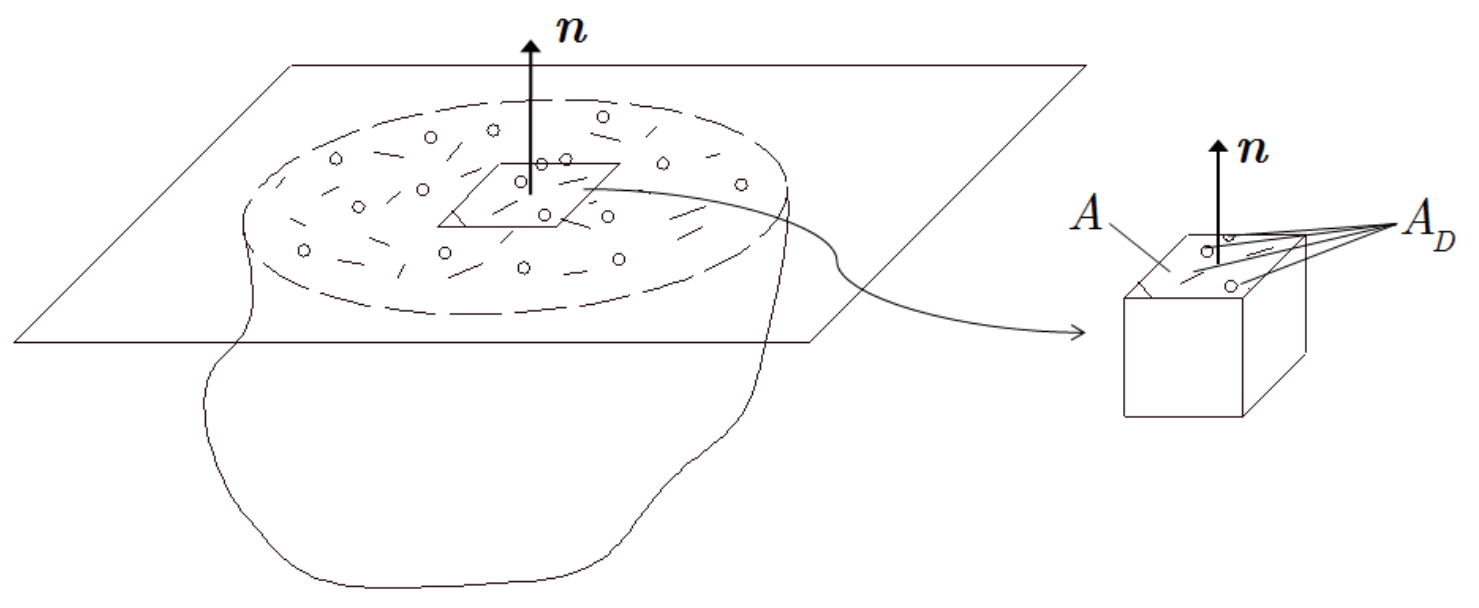
\includegraphics[width=0.65\textwidth]{./Figures/damageModels/damageVolume.png}
%\caption{Representaive volume element isolated from a damaged body \cite{voyiadjis_damage_2005}}
%\label{fig:RVEDamage}
%\end{center}
%\end{figure}
%
%For the representative volume element (RVE), $A_D$ is equal to the area occupied by defects, A is equal to the remaining area of the surface and $A_o$ is the original area of the surface, prior to the development of micro voids and micro-cracks. The damage variable is then given by:
%\begin{equation}
%	D=\frac{A_o\ -\ A}{A_o}=\frac{A_d}{A_o}	
%\end{equation}

% When no damage has taken place, the damage variable is, therefore, equal to 0 (virgin material), whereas when the material is equal to 1 this corresponds to the fully damaged material. From a physical point of view, the variable $D$ is the corrected area of cracks and cavities per unit surface cut by a plane perpendicular to $\mathbf{n}$. 
%From this definition of damage follows the concept of the effective stress. Let us consider a uniaxial case where a force $F$ is applied to the RVE. The stress is given by:
%\begin{equation}
%	\sigma=\frac{F}{A_o}	
%\end{equation}
%
%After the development of damage, however, the surface area of the macroscale volume which the force $F$ acts upon is reduced. The effective area is given in terms of the original area and the damage variable is as follows:
%\begin{equation}
%	\frac{A_o\ -\ A}{A_o}=D	
%\end{equation}
%\begin{equation}
%	A_o\ -\ A=DA_o	
%\end{equation}
%\begin{equation}
%	\frac{A_o\ -\ A}{A_o}=D	
%\end{equation}
%\begin{equation}
%	A=\left(1-D\right)A_o	
%\end{equation}
% The effective stress is then determined by combining this relation with the equation for the stress (equation 4.7):
% \begin{equation}
%	\bar{\sigma}\ =\frac{F}{{\left(1-D\right)A}_o}=\frac{\sigma}{\left(1-D\right)}	
%\end{equation}
%Based on these macroscopic considerations, Lemaitre \cite{lemaitre_continuous_1985} developed a thermodynamically consistent model.

%\subsection{Thermodynamic framework}

%
%The Lemaitre damage model described herein is coupled with the isotropic plasticity model laid out in chapter 3. In the Lemaitre model, a free energy potential $\psi$ is postulated from which the state laws are derived. The free energy is expressed as a function of the elastic strain $\boldsymbol{\varepsilon}^e$, the hardening variable $a$ and the damage variable D in the form:
% \begin{equation}
%	\psi=\psi\left(\boldsymbol{\varepsilon}^e,\alpha,D\right)
%\end{equation}
%The free energy potential can be decomposed into its elastic-damage and plastic contributions:
% \begin{equation}
%	\psi\left(\boldsymbol{\varepsilon}^e,\alpha,D\right)=\psi^{ed}\left(\boldsymbol{\varepsilon}^e,D\right)+\psi^p\left(\alpha\right)
%\end{equation}
%Where $\psi^{ed}$ and $\psi^p$ are the elastic-damage and plastic energy contributions respectively. The elastic-damage potential is assumed to be:
% \begin{equation}
%	\bar{\rho}\psi^{ed}=\frac{1}{2}\boldsymbol{\varepsilon}^e:\mathbf{D}^{e}\left(1-D\right):\boldsymbol{\varepsilon}^e	
%\end{equation}
%
%The Kirchhoff stress tensor is obtained by finding the derivative with respect to the elastic strain (section 3.2.1):
% \begin{equation}
%	\boldsymbol{\tau}=\bar{\rho}\frac{\partial\psi^{ed}}{\partial\boldsymbol{\varepsilon}^e}=\mathbf{D}^{e}\left(1-D\right):\boldsymbol{\varepsilon}^e	
%	\end{equation}
%
%The energy release rate Y, which gives the energy dissipated due to the phenomenon of damage, is given by:
% \begin{equation}
%	Y=\bar{\rho}\frac{\partial\psi^{ed}}{\partial D}=-\frac{1}{2}\boldsymbol{\varepsilon}^e:\mathbf{D}^e:\boldsymbol{\varepsilon}^e
%\end{equation}
%This can equivalently be written as:
% \begin{equation}
%	Y=-\frac{1}{2}\bar{\boldsymbol{\tau}}:{\mathbf{D}^e}^{-1}:\bar{\boldsymbol{\tau}}
%\end{equation}
%With some algebraic manipulation \cite{lemaitre_engineering_2005}:
% \begin{equation}
% \label{eqn:classicY}
%	Y=-\frac{{\bar{\tau}_{eq}}^2}{2E}\left(\frac{2}{3}\left(1+v\right)+3\left(1-2v\right)\left(\frac{\tau_h}{\tau_{eq}}\right)^2\right)	
%\end{equation}
%where $E$ is the Young's modulus and $v$ is Poisson's ratio. The triaxiality dependence of the Lemaitre mode is provided by the term $\frac{\tau_h}{\tau_{eq}}$, which is the definition of stress triaxiality $\eta$. The state potential associated with the isotropic hardening variable is given by: 
% \begin{equation}
%	\chi=\rho\frac{\partial\psi^p}{\partial \alpha}
%	\end{equation}
%
%The hardening variable $\alpha$ is commonly chosen as the equivalent plastic strain denoted by ${\bar{\varepsilon}}^p$. 
%The Clausius-Duhem inequality (equation 3.28) is rewritten to incorporate the damage $D$ and its associated thermodynamic force $Y$ to give:
%\begin{equation}
%\boldsymbol{\tau}:\bar{\mathbf{d}}^p-\chi\dot{\alpha}-Y\dot{D}\geq0
%\end{equation}

%%%%%%%%%%%%%%%%%%%
\subsection{Lemaitre damage model}
%%%%%%%%%%%%%%%%%%%

\subsubsection{Model Formulation}

The Lemaitre model describes damage using a scalar field variable $D$.
When no damage has occurred, the damage variable $D$ equals 0 (virgin material), whereas when the material is fully damaged, the damage variable equals 1.
From a physical point of view, $D$ can be interpreted as the area of cracks and cavities per unit surface cut by an arbitrary plane.
% perpendicular to $\mathbf{n}$. 

%The Lemaitre model is formulated by assuming a dissipation potential $F$:
% \begin{equation}
%	F = F_p + F_d	
%\end{equation}
%where $F_p$ and $F_d$ are the dissipation potentials associated with plasticity and damage, respectively. The plastic potential is given by the $J_2$ (von Mises) yield criterion:
% \begin{equation}
%	F_p = \frac{\sigma_{v}}{1 - D} \; - \; \sigma_y\left(\alpha\right)	
%\end{equation}
%The yield stress $\sigma_y$ is a function of the hardening variable $\alpha$, taken here to represent the equivalent plastic strain.
%
%The damage dissipation potential is given by \citet{lemaitre_continuous_1985}:
% \begin{equation}
%	F_d = \frac{S_0}{\left(b + 1\right) \left(1 - D\right)}\left(\frac{-Y}{S_0}\right)^{b+1}
%\end{equation}
%where $S_0$ and $b$ are material parameters governing the onset and rate of damage.

%Plastic isotropy is assumed and, in order to ensure that dissipation is always
%positive, the Kuhn-Tucker conditions must always hold at every material point:
%\begin{equation}
%\left\{\begin{array}{c}
%\dot{\gamma}=\geq 0 \\
%F\geq 0 \\
%\dot{\gamma}F=0
%\end{array}\right.
%\end{equation}

The Lemaitre model augments the elastoplasticity constitutive law (Equations \ref{eq:yieldFunc} and \ref{eq:flowRule}) with the inclusion of a damage variable $D$ evolution law, and scaling of the yield function and flow rules by the reciprocal of $(1 - D)$:
% can then be given in terms of the spatially rotated plastic stretch $\bar{\mathbf{d}}_p$ (or plastic deformation gradient rate $\dot{\mathbf{F}_p}$), the hardening variable rate $\dot{\alpha}$, and damage variable rate $\dot{D}$:
 \begin{eqnarray} \label{eq:lemaitre_dp}
	 \Phi &=& \frac{\sigma_v}{1 - D} \; - \; \sigma_y\left(\bar{\varepsilon}_p \right) \\
    \dot{\mathbf{F}}_p \cdot \mathbf{F}_p^{-1}
    &=&
    \frac{\dot{\bar{\varepsilon}}_p}{1 - D} \; \mathbf{R}_e^T \cdot 
    \left[
    \frac{3}{2} \frac{\text{dev}\left(\boldsymbol{\sigma} \right)} {\sigma_{v}}
    \right]
    \cdot  \mathbf{R}_e \\
    \dot{D} &=&
    %-\dot{\gamma}\frac{\partial F}{\partial Y}
    \frac{\dot{\bar{\varepsilon}}_p}{1 - D}\left(\frac{-Y}{S_0}\right)^b \label{eq:lem_damage}
\end{eqnarray}
% \begin{equation}
%	\dot{\alpha} = -\dot{\gamma}\frac{\partial F}{\partial\chi}=\dot{\gamma}
%\end{equation}
% \begin{equation}
%	\dot{D} = -\dot{\gamma}\frac{\partial F}{\partial Y}=\frac{\dot{\gamma}}{\left(1 - D\right)}\left[\frac{-Y}{S_0}\right]^b
%\end{equation}
%We can equivalently write the rate of plastic strain (Equation \ref{eq:lemaitre_dp}) in terms of the multiplicative plastic deformation gradient $\mathbf{F}_p$ as
%\begin{equation}
%	\dot{\mathbf{F}_p} \mathbf{F}_p^{-1} =
%	\frac{3}{2} \frac{\dot{\gamma}}{1 - D} \mathbf{R}_e^{T} \frac{\text{dev}(\boldsymbol{\tau})}{\sigma_{v}} \mathbf{R}_e
%\end{equation}
where $S_0$ (dimensions of stress) and $b$ (dimensionless) are material parameters.
The energy release rate $Y$, which gives the energy dissipated due to the phenomenon of damage, is given by \cite{lemaitre_engineering_2005}
% \begin{equation}
%	Y
%	%= \bar{\rho}\frac{\partial\psi^{ed}}{\partial D}
%	= -\frac{1}{2} \boldsymbol{\varepsilon}_e : \mathbf{D}_e : \boldsymbol{\varepsilon}_e
%\end{equation}
%which can equivalently be written as
% \begin{equation}
%	Y=-\frac{1}{2}\bar{\boldsymbol{\tau}}:{\mathbf{D}^e}^{-1}:\bar{\boldsymbol{\tau}}
%\end{equation}
%With some algebraic manipulation \cite{lemaitre_engineering_2005}:
\begin{equation} \label{eqn:classicY}
	Y
	=
%	-\frac{{\bar{\tau}_{eq}}^2}{2E}
	-\frac{\sigma_v^2}{2E}
	\left[
%	\frac{2}{3} (1 + v) + 3 (1 - 2v) \left( \frac{p}{\sigma_v} \right)^2
	\frac{2}{3} (1 + \nu) + 3 (1 - 2\nu) \eta^2
	\right]
\end{equation}
where $E$ is Young's modulus and $\nu$ is Poisson's ratio, where the dependence on triaxiality ($\eta = \sfrac{p}{\sigma_{v}}$) is explicitly clear.
%The triaxiality dependence of the Lemaitre mode is provided by the term $\frac{\tau_h}{\tau_{eq}}$, which is the definition of stress triaxiality $\eta$.
%The state potential associated with the isotropic hardening variable is given by: 
% \begin{equation}
%	\chi=\rho\frac{\partial\psi^p}{\partial \alpha}
%\end{equation}


\paragraph{Triaxiality and Lode Angle Dependence}

The classic Lemaitre model does not distinguish between positive and negative triaxiality ($\eta$ is squared in Equation \ref{eqn:classicY}); consequently, it can overpredict damage in wire drawing processes where triaxiality can be highly negative.
%it tends to predict fracture too early at low triaxialities and too late at high triaxialities. 
%Physically, highly negative triaxiality (highly positive hydrostatic pressure) is known to suppress damage formation.
A simple remedy is to employ a triaxiality cut-off \cite{bouchard_enhanced_2011}, which disallows damage evolution for highly negative triaxiality values:
\begin{equation} \label{eq:triaxCutoff} % note: flip sign from Andrew's thesis, as Andrew assume p = hyd(sigma), whereas we assume p = -hyd(sigma)
	\dot{D} =
	\begin{cases}
		0 & \text { if } \eta \leq -\frac{1}{3}  \\
		\frac{\dot{\bar{\varepsilon}}_p}{1 - D}\left(\frac{-Y}{S_0}\right)^b 
		& \text { if } \eta>-\frac{1}{3}
	\end{cases}
\end{equation}



 %at which point the cell is assumed to be fully damaged.

% The damage is not set to $1$ to allow for some residual stresses in this cell to aid convergence.
%\begin{equation}
%\label{DamageUpdateEquation}
%D^{i+1}^{[m+1]}= \begin{cases} D_n+\frac{\Delta\gamma}{\left(1-D^{i}^{[m+1]}\right)}\left[\frac{-Y^{[m+1]}}{r}\right]^s & \text { if } D^{i}^{[m+1]}<D_c \\ 0.99 & \text { if } D^{i}^{[m+1]} \geq D_c \end{cases}
%\end{equation}


%Various alternative formulations of the Lemaitre damage model have been proposed in the literature.
%Typically, these models entail an alteration of the damage dissipation potential \cite{cao_lode-dependent_2014,chandrakanth_isotropic_1995,wei_hua_tai_new_1986,bouchard_enhanced_2011,bonora_nonlinear_1997,malcher_improved_2014,ferreira_improved_2022,castro_calibration_2018,lian_modified_2014} and therefore, following the procedure described in section 4.2.3, an alternative damage evolution equation is derived. 

Rather than use a triaxiality cut-off, Malcher and co-workers \citep{malcher_improved_2014, ferreira_improved_2022, castro_calibration_2018} proposed that the parameter $S_0$ be a function of triaxiality $\eta$ as well as Lode angle $\xi$.
%Of particular interest in this work is the class of models based on the formulation developed by \citet{malcher_improved_2014}.
This approach has shown an ability to accurately predict fracture for a range of loading conditions, at both low and high triaxiality values and for various shear stress states.
The Malcher et al. form of damage evolution is achieved by making $S_0$ in Equation \ref{eq:lem_damage} a function of $\eta$ and $\xi$:
\begin{equation}
S(\eta,\xi)=\frac{S_{0.33}}{3|\eta|+\frac{S_{0.33}}{S_{0.0}}\left(1-\xi^2\right)}
\end{equation}
where $S_{0.33}$ and $S_{0.0}$ are material parameters, which were determined based on pure tensile loading $S_{0.33}$ and pure shear loading ($S_{0.0}$).

%As noted in \citet{malcher_improved_2014}, 
%To remedy this, an alternative damage dissipation potential was proposed: 
%\begin{equation}
%	F_{D}=\frac{S(\eta,\xi)}{\left(1-D\right)\left(b+1\right)}\left[\frac{-Y}{S(\eta,\xi)}\right]^{b+1}
%\end{equation}
% Following the procedure described in section 4.2.3 of this thesis, the damage evolution equation is then given as:
%
% \begin{equation}
%	\dot{D}=\frac{\dot{\gamma}}{\left(1-D\right)}\left[\frac{-Y}{S(\eta,\xi)}\right]^b
%\end{equation}
%The Lemaitre damage denominator is modified to become a function of the triaxiality $\eta$ and in some cases the normalised third invariant $\xi$. The damage denominator is given by \citet{malcher_improved_2014} as:

Despite its success, one weakness of this formulation is that it does not distinguish between positive and negative triaxiality values, which is critical for wire drawing.
%In Chapter 7, a novel Lemaitre damage model is proposed in this work that is conceptually similar to the above formulation.
To overcome this limitation, a function for $S(\eta,\xi)$ is proposed here, inspired by the Ko criterion \cite{ko_prediction_2007} uncoupled damage law.
The Ko criterion has shown an ability to predict fracture in both wire drawing processes \cite{roh_process_2021} and in the hub-hole expanding process \cite{ko_prediction_2007}.
For the wire drawing, $\xi\approx1.0$ at the wire centre, where fracture originates \cite{roh_process_2021}.
For this reason, the proposed function does not incorporate a dependency on $\xi$, and final expression for $S$ takes the form
\begin{equation} \label{eqn:proposedLemaitre}
	S(\eta) = \frac{2S_0}{\left(1.0+3\eta\right)}
\end{equation}

%For the wire drawing cases to be looked at in this chapter $\xi\approx1.0$ at the centre of the wire (Appendix F.1) where fracture originates \cite{roh_process_2021}. For this reason, the proposed function does not incorporate a dependency on $\xi$. The damage evolution law can be rewritten as:
%\begin{equation}
%	\dot{D}=\frac{\dot{\gamma}}{1-D}\left[\frac{-Y}{2S_0}\left(1.0+3\eta\right)\right]^b
% \end{equation}



\paragraph{Crack Closure Effects}

An additional limitation of the classic Lemaitre damage model is that it does not distinguish between tensile and compressive stress states, whereas it is known from experiments that tensile stresses are considerably more conducive to crack growth than compressive stresses \cite{bao_cut-off_2005}.
To overcome this shortcoming, some authors assume no crack growth in compressive stress states \cite{chu_void_1980}; however, this does not account for the partial closure of micro-defects under compressive stress states.; this effect causes a greater material area to bear the compressive load.
As a result, the material may exhibit a partial or complete recovery of its stiffness, depending on the specific conditions \cite{teixeira_ductile_2010}.
This approach also does not account for the fact that some crack growth can occur in compressive stages \cite{basic_finite_2005}.

Consequently, an \emph{enhanced} Lemaitre model with crack closure effects has been proposed \cite{pires_issues_2005,teixeira_ductile_2010}.
% can be used to more accurately account for damage development.
In this approach, the energy release rate $Y$ (Equation \ref{eqn:classicY}) is rewritten to account for the differing contributions of tensile and compressive stresses:
\begin{eqnarray}
	Y &=&
	\frac{-1}{2E\left(1-D\right)}
	\left[(1 + \nu) \bb{\sigma}^+ : \bb{\sigma}^+ - \nu\ \langle \text{tr}(\boldsymbol{\sigma})\rangle^2\right] \notag \\
	&&-\frac{h}{2E\left(1-hD\right)}
	\left[(1 + \nu)\bb{\sigma}^- : \bb{\sigma}^- -\nu \langle -\text{tr}(\boldsymbol{\sigma})\rangle^2\right]
\end{eqnarray}
where Macaulay brackets are indicated by $\langle \bullet \rangle$.
%Under compressive stress, micro-cracks will partially or fully close, leading to an increase in the load-carrying area.
The parameter $0\le h\le1$ accounts for the crack closure phenomenon; here, we take $h = 0.2$ as is common for steels \cite{desmorat_modeling_2008,lemaitre_course_1996,bouchard_enhanced_2011}). 
%In this model, an effective stress for compressive stress states is introduced. It differs from that in equation 4.12 through the introduction of the material parameter $h$ (and given here in terms of the Kirchhoff stress):
%\begin{equation}
%	\bar{\boldsymbol{\tau}}\ =\frac{\boldsymbol{\tau}}{\left(1-hD\right)}	
%\end{equation}
%An eigendecomposition is performed to split the stress tensor into its positive and negative components
%\begin{equation}
%	\boldsymbol{\sigma} \;=\; \boldsymbol{\sigma}^+ \;+\; \boldsymbol{\sigma}^-
%\end{equation}
The positive and negative stress components are defined as
\begin{eqnarray}
	\boldsymbol{\sigma}^+&=&\sum_{i=1}^{3} \langle{\sigma}_i \rangle\mathbf{e}_i\otimes\mathbf{e}_i	\\
	\boldsymbol{\sigma}^-&=&\sum_{i=1}^{3}\langle{-{\sigma}}_i\rangle\mathbf{e}_i\otimes\mathbf{e}_i
\end{eqnarray}
where ${\sigma}_i$ are the principal stresses, $\{\mathbf{e}_1,\mathbf{e}_2,\mathbf{e}_3\}$ are the orthonormal basis vectors, and $\boldsymbol{\sigma} = \boldsymbol{\sigma}^+ + \, \boldsymbol{\sigma}^-$.
%$\otimes$ is the outer product and $<>$ is a Macauley bracket.
%The effective stress tensor can then be given by:
%\begin{equation}
%	\bar{\boldsymbol{\tau}}\ =\frac{\boldsymbol{\tau}_+}{\left(1-D\right)}+\frac{\boldsymbol{\tau}_-}{\left(1-hD\right)}	
%\end{equation}

%For the sake of numerical efficiency, 
A simplified form of the crack-closure model \cite{teixeira_ductile_2010} is employed in this work, whereby this definition of decomposed stress is only used in the damage evolution calculation. 






\paragraph{Non-Local Damage}

%It is worth noting the benefit of the developed implicit-explicit algorithm when looking at this class of models. The fact that the developed algorithm does not require the solution of the damage implicitly means that incorporating novel damage evolution equations into the existing code is relatively simple, without the need to calculate derivatives that can become quite complex when incorporating shear effects, in particular, \cite{malcher_improved_2014}.

One limitation of damage models is that due to the strain softening behaviour, prediction may suffer from mesh size and orientation dependency in localised strain zones \cite{peerlings_critical_2001, peerlings_localisation_2002, geers_strongly_2003}.
%The governing differential equations can lead to multiple possible solutions due to the nonlinearity and softening response.
%The finite element or volume solution process may converge to one of these possible solutions depending on factors like the mesh, boundary conditions, or solver parameters. This brings the uniqueness of the solution into question.
To rectify this, an implicit \emph{non-local} damage variable $\bar{D}$ is introduced as in \citet{peerlings_critical_2001, peerlings_localisation_2002} and \citet{geers_strongly_2003}.
This is related to the local damage variable $D$ through the implicit diffusion equation:
\begin{equation} \label{eqn:nonLocalEquation}
	\bar{D} -  l_c^2 \bb{\nabla}^2 \bar{D} = D
\end{equation}
where $l_c$ is a characteristic length scale which controls the area over which the local damage is diffused.
This equation can be viewed as a smoothing equation ($\bar{D}$ is a spatially smoothed version of $D$), which has the effect of mitigating the mesh dependency. This equation is solved with the zero-flux Neumann boundary conditions on all boundaries:  $\bb{n} \cdot \nabla \bar{D} = 0$.
%\begin{equation}
%    \nabla \bar{D}\cdot\textbf{n}=0 
%\end{equation}
The terms in Equation \ref{eqn:nonLocalEquation} are discretised using the cell-centred finite volume method, similar to the pressure equation (Equation \ref{eq:pressureEqn}).

%The Algorithm for incorporating the non-local damage is provided in Algorithm 4. As can be seen, the procedure is very similar to that in the local Lemaitre damage model. Algorithm 4 is provided to clarify how the non-local damage is coupled with the elasto-plastic model and the steps involved prior to solving the non-local damage gradient equation.


\subsubsection{Computational Procedure}
%For each cell, the incremental displacement field $\Delta\boldsymbol{u}$ for the current time step $t^{[m+1]}$, at the current iteration, is provided. The following variables from the previous time step are also given:
% \begin{equation}
%\left\{F_n^p,\ \alpha_n,D_n\right\}
%\end{equation}
%The goal is then to have a return-mapping algorithm to obtain the following variables at time $t^{[m+1]}$
%\begin{equation}
%\left\{F^{[m+1]}^p,\ \alpha^{[m+1]},\boldsymbol{\sigma}^{[m+1]},D^{[m+1]}\right\}
%\end{equation}
%In order to obtain these values, the algorithm must satisfy the following constitutive behaviour:
%\begin{equation}
%\label{eqn:deformationPlasticStrainRelation}
%	{\dot{\mathbf{F}}}^p\mathbf{F}^{p-1}=\frac{3}{2}\frac{\dot{\gamma}}{\left(1-D\right)}\mathbf{R}^{eT}\frac{\boldsymbol{\tau}_d}{\tau_{eq}}\mathbf{R}^e={\bar{\mathbf{d}}}^p
%\end{equation}
%\begin{equation}
%	\dot{\alpha}=\dot{\gamma}	
%\end{equation}
%\begin{equation}
%	\dot{D}=-\dot{\gamma}\frac{\partial F}{\partial Y}=\frac{\dot{\gamma}}{\left(1-D\right)}\left[\frac{-Y}{S_0}\right]^b
%\end{equation}



%Equation \ref{eqn:deformationPlasticStrainRelation} is integrated using the one-step implicit integration operator corresponding to the Euler backward method to get:
%\begin{equation}
%	\mathbf{F}^{[m+1]}^p=exp\left[\frac{3}{2}\frac{\Delta\gamma}{\left(1-D^{[m+1]}\right)}\mathbf{R}^{[m+1]}^{e^T}\frac{\boldsymbol{\tau}_{d^{[m+1]}}}{\tau_{eq\ n+1}}\mathbf{R}^{[m+1]}^e\right]\mathbf{F}^{[m]}^p
%\end{equation}
%Following the procedure laid out in section 3.2.3, the additive split for the elastic and plastic strain is obtained:
%\begin{equation}
%	\boldsymbol{\varepsilon}^{[m+1]}^e=\boldsymbol{\varepsilon}^{[m+1]}^{e\ trial}-\frac{3}{2}\frac{\Delta\gamma}{\left(1-D^{[m+1]}\right)}\frac{\boldsymbol{\tau}_{d^{[m+1]}}}{\tau_{eq\ n+1}}
%\end{equation}
%
%The integration of the other constitutive equations using the backwards Euler scheme is simply given by:
%\begin{equation}
%	\alpha^{[m+1]}-\alpha_n=\Delta\gamma
%\end{equation}
%\begin{equation}
%   \alpha^{[m+1]}=\alpha_n+\Delta\gamma	
%\end{equation}
%\begin{equation}
%	D^{[m+1]}-D_n=\frac{\Delta\gamma}{\left(1-D^{[m+1]}\right)}\left[\frac{-Y^{[m+1]}}{S_0}\right]^b
%\end{equation}
%\begin{equation}
%D^{[m+1]}=D_n+\frac{\Delta\gamma}{\left(1-D^{[m+1]}\right)}\left[\frac{-Y^{[m+1]}}{S_0}\right]^b	
%\end{equation}
%
%The final system of equations to be solved when the material is undergoing plastic straining is therefore given by:
%
%\begin{equation}
%\left\{\begin{array}{c}
%\frac{\tau_{eq\ n+1}}{1-D^{[m+1]}}-\sigma_y\left(\alpha^{[m+1]}\right)=0 \\
%\boldsymbol{\varepsilon}^{[m+1]}^e=\boldsymbol{\varepsilon}^{[m+1]}^{e\ trial}-\frac{3}{2} \frac{\Delta \gamma}{1-D^{[m+1]}} \frac{\boldsymbol{\tau}_{d^{[m+1]}}}{\tau_{eq\ n+1}}\\
%\alpha^{[m+1]}=\alpha_n+\Delta \gamma \\
%D^{[m+1]}=D_n+\frac{\Delta\gamma}{\left(1-D^{[m+1]}\right)}\left[\frac{-Y^{[m+1]}}{S_0}\right]^b
%\end{array}\right. 
%\end{equation}


An implicit-explicit algorithm is developed in this work to solve Equations \ref{eq:lemaitre_dp}-\ref{eq:lem_damage}.
At every outer iteration, the plastic increment is solved implicitly, with the value for the damage variable fixed from the previous outer iteration.
The damage rate equation (Equation \ref{eq:lem_damage}) is then solved in a \emph{deferred-correction} manner using the damage from the previous iteration ($\bar{D}_{[i]}$, where $[i]$ indicate a value from a previous outer iteration).
This approach avoids the use of a $2 \times 2$ matrix (or an even higher dimension matrix if one was to solve for anisotropic plasticity or plasticity incorporating kinematic hardening) that would be needed if both the damage and the plastic increment were solved for implicitly simultaneously.
By not requiring the solution of both the plasticity and damage simultaneously, the mathematics are simplified when solving for more complex formulations of the Lemaitre damage evolution equation and for the \emph{non-local damage}, which will be described later in this section.
Note that the overall solution algorithm is still implicit in time.

%The superscript notation laid out in equations \ref{eqn:superscript1} and \ref{eqn:superscript2} is used to indicate whether the damage variable is from the current iteration or from the previous iteration. The superscript $^{i+1}$ means that the variable is from the current outer iteration while the superscript $^{i}$ means that the variable is from the previous outer iteration.
%
%\begin{equation}
%\label{eqn:superscript1}
%    D^{i+1}^{[m+1]}
%\end{equation}
%\begin{equation}
%\label{eqn:superscript2}
%    D^{i}^{[m+1]}
%\end{equation}

%The first three of the equations in the system given in 4.41 can be satisfied by solving the yield potential for the plastic increment $\Delta\gamma$, with the damage obtained from the previous iteration frozen. 

%First, the von Mises stress is defined in terms of the elastic strain and combined with equation 4.36:
%\begin{equation}
%\begin{aligned}
%%\frac{\tau^{eq}^{[m+1]}}{1-D^{i}^{[m+1]}}=\bar{\tau}_{{eq}^{[m+1]}}&=\sqrt{\frac{3}{2}}\left\|2 \mu \operatorname{dev}\left(\boldsymbol{\varepsilon}^{[m+1]}^e\right)\right\|\\
%%&=\sqrt{\frac{3}{2}}\left\|2 \mu \operatorname{dev}\left(\boldsymbol{\varepsilon}^{[m+1]}^{e \text { trial }}-\frac{3}{2} \frac{\Delta \gamma}{\left(1+D^{i}^{[m+1]}\right)} \frac{\boldsymbol{\tau}_{d^{[m+1]}}}{\tau_{eq\ n+1}}\right)\right\|
%fix
%\end{aligned}
%\end{equation}

%Following the procedure laid out in Section 3.2.3, the equation for the yield function in terms of the plastic increment can be obtained in terms of the plastic increment:
%\begin{equation}
%	\bar{\tau}_{eq\ n+1}^{trial}-3\mu\frac{\Delta\gamma}{\left(1-D^{i}^{[m+1]}\right)}-\sigma_{y\ }\left(\alpha_n+\Delta\gamma\right)=0
%\end{equation}

%This is solved implicitly using the Newton-Raphson algorithm for $\Delta\gamma$; the stress tensor and the plastic strain tensor are then updated based on this value.  
%After updating these values, the damage equation can be solved explicitly.


%\paragraph{Overall Stress Calculation Procedure}

This stress calculation procedure for the Lemaitre damage model is summarised in Algorithm \ref{alg:lemaitre}, where $\bar{D}^{[m+1]}_{[i]}$ is the latest available non-local damage field at the new time, i.e. its values from the previous outer iteration; at convergence within each time step, $\bar{D}^{[m+1]}_{[i]}$ becomes $\bar{D}^{[m+1]}_{[i+1]} \equiv \bar{D}^{[m+1]}$.
As shown, to aid numerical convergence, a critical damage parameter $D_c$ is incorporated \cite{lemaitre_continuous_1985}, which limits the maximum value of the damage $D$ to $D_c$, rather than $1$.
In the current work, $D_c = 0.99$ is assumed.
Consequently, the damage rate equation (Equation \ref{eqn:classicY}) becomes
\begin{equation} \label{eq:damageLimit} % note: flip sign from Andrew's thesis, as Andrew assume p = hyd(sigma), whereas we assume p = -hyd(sigma)
%	D^{i+1}^{[m+1]}= \begin{cases}D_n & \text { if } \eta\leq-\frac{1}{3}	\\
%	D_n+\frac{\Delta\gamma}{\left(1-D^{i}^{[m+1]}\right)}\left[\frac{-Y^{[m+1]}}{r}\right]^s & \text { if } \eta>-\frac{1}{3}\end{cases}
	\dot{D} =
	\begin{cases}
		0 & \text { if } \eta \leq -\frac{1}{3} \text{ or } D \geq D_c \\
		\frac{\dot{\bar{\varepsilon}}_p}{1 - D}\left(\frac{-Y}{S(\eta,\xi)}\right)^b 
		& \text { if } \eta>-\frac{1}{3} \text{ and }  D < D_c
	\end{cases}
\end{equation}
where $S$ can be a function of $\eta$ and $\xi$ as described above.
%In addition, $D$ is explicitly bound to be less than of equal to $D_c$.

\begin{algorithm}[htbp] \label{alg:lemaitre} \footnotesize
\SetAlgoLined
(i) Update deformation gradients for a given incremental displacement

\begin{equation}
  \mathbf{f}^{[m+1]} = \mathbf{I} + \left[ \bb{\nabla}(\Delta\textbf{u}) \right]^T \nonumber
\end{equation}

\begin{equation}
  \mathbf{F}^{[m+1]} = \mathbf{f}^{[m+1]} \cdot \mathbf{F}^{[m]}  \nonumber
\end{equation}

(ii) Compute trial elastic state
\begin{equation}
\mathbf{B}_{e}^{[m]} = \exp\left({2\boldsymbol{\varepsilon}_{e}^{[m]}}\right) \nonumber
\end{equation}
\begin{equation}
\mathbf{B}_{e}^{\text{trial}} = \mathbf{f}^{[m+1]} \cdot \mathbf{B}_{e}^{[m]} \cdot (\mathbf{f}^{[m+1]})^{T}\nonumber
\end{equation}
\begin{equation}
\boldsymbol{\varepsilon}_{e}^{\text{trial}} = \frac{1}{2} \ln(\textbf{B}_{e}^{\text{trial}}) \nonumber
\end{equation}
\begin{equation}
\bar{\varepsilon}^{\text{trial}}_p = \bar{\varepsilon}^{[m]}_p \nonumber
\end{equation}
\begin{equation}
\sigma_{v}^{\text{trial}} = \sqrt{\sfrac{3}{2}} || 2G\ \text{dev}(\boldsymbol{\varepsilon}_{e}^{\text{trial}})|| \nonumber
\end{equation}
\hl{Andrew: should the yield function include D old (equation 26)?}
\begin{equation}
%\Phi^{\text{trial}} =  \frac{\sigma_{v}^{\text{trial}}}{1 - \bar{D}^{[m]}} - \sigma_{y}(\bar{\varepsilon}^{\text{trial}}_p) \nonumber 
\Phi^{\text{trial}} =  \sigma_{v}^{\text{trial}} - \sigma_{y}(\bar{\varepsilon}^{\text{trial}}_p) \nonumber 
\end{equation}
  \eIf{$\Phi^{\text{trial}} > 0$}{
   go to step (iii) to solve for $\Delta\bar{\varepsilon}_p$
   }{
   $\Delta\bar{\varepsilon}_p = 0$ and go to step (iv)
  }

(iii) Use the Newton-Raphson method to solve the yield function for $\Delta\bar{\varepsilon}_p$:
\begin{equation}
	\sigma_{v}^{\text{trial}} 
	- \frac{ 3\mu \Delta\bar{\varepsilon}_p }{1 - \bar{D}^{[m+1]}_{[i]}}
	-\sigma_{y}(\bar{\varepsilon}^{[m]}_p + \Delta\bar{\varepsilon}_p) = 0 \nonumber
\end{equation}

(iv) Update constitutive variables and deviatoric stress
\begin{equation}
	\boldsymbol{\varepsilon}_{e}^{[m+1]}
	=
	\boldsymbol{\varepsilon}_{e}^{\text{trial}}
	- \sqrt{\frac{3}{2}} \; \frac{ \Delta\bar{\varepsilon}_p}{1 - \bar{D}^{[m+1]}_{[i]}}
	\frac{\text{dev}(\boldsymbol{\varepsilon}_{e}^{\text{trial}})}{||\boldsymbol{\varepsilon}_{e}^{\text{trial}}||}
	\nonumber
\end{equation}
\begin{equation}
	\bar{\varepsilon}_p^{[m+1]} = \bar{\varepsilon}_p^{[m]} + \Delta\bar{\varepsilon}_p \nonumber
\end{equation}

\begin{equation}
%	\boldsymbol{\sigma}^{[m+1]} = \frac{1}{J} \mathbf{D}^e:\boldsymbol{\varepsilon}^{e} \nonumber
	\boldsymbol{s}^{[m+1]}
	=
	\left(1 - \bar{D}^{[m+1]}_{[i]}\right) (\sfrac{1}{J}) 2\mu \;\text{dev}\left(\boldsymbol{\varepsilon}_{e}^{[m+1]}\right) \nonumber
\end{equation}

(v) Implicitly solve the pressure Poisson's equation, where $J^{[m+1]} = -(1 - \bar{D}^{[m+1]}_{[i]}) \kappa \; \text{tr}\left(\boldsymbol{\varepsilon}_{e}^{[m+1]}\right)$.
\begin{equation}
	p^{[m+1]} - \mathbb{D} \bb{\nabla}^2 p^{[m+1]} = -\frac{\kappa}{2} \left[\left(J^{[m+1]}\right)^{2} - 1\right] - \bb{\nabla} \cdot \left( \mathbb{D} \bb{\nabla} p^{[m+1]}_{[i]} \right)
\end{equation}


(vi) Update the true (Cauchy) stress
\begin{equation}
	\boldsymbol{\sigma}^{[m+1]} = \boldsymbol{s}^{[m+1]} -  p^{[m+1]}\textbf{I} \nonumber
\end{equation}

(vii) Update the local damage (use the modified form for $Y$ if the crack $h > 0$)
%\ref{eq:triaxCutoff} and \ref{eq:damageLimit}
\begin{equation} % note: flip sign from Andrew's thesis, as Andrew assume p = hyd(sigma), whereas we assume p = -hyd(sigma)
	D^{[m+1]} =
	\begin{cases}
		D^{[m]} & \text { if } \eta \leq -\frac{1}{3} \text{ or } D^{[m+1]}_{[i]} \geq D_c \\
		\text{max} \left[ D^{[m]} + \frac{\dot{\bar{\varepsilon}}_p}{1 - D^{[m+1]}_{[i]}}\left(\frac{-Y}{S(\eta,\xi)}\right)^b, \; D_c \right]
		& \text { if } \eta>-\frac{1}{3} \text{ and }  D^{[m+1]}_{[i]} < D_c
	\end{cases}
\end{equation}


(vii) Implicitly solve diffusion equation for non-local damage
\begin{equation}
	\bar{D}^{[m+1]} -  l_c^2 \bb{\nabla}^2 \bar{D}^{[m+1]} = D^{[m+1]}
\end{equation}

(viii) Limit the non-local damage
\begin{equation}
	\bar{D}^{[m+1]} = \text{max} \left( \bar{D}^{[m+1]} , D_c \right)
\end{equation}

\caption{Lemaitre damage model stress calculation algorithm}
\end{algorithm}
\normalsize

%\begin{figure}[htb]
%\begin{center}
%	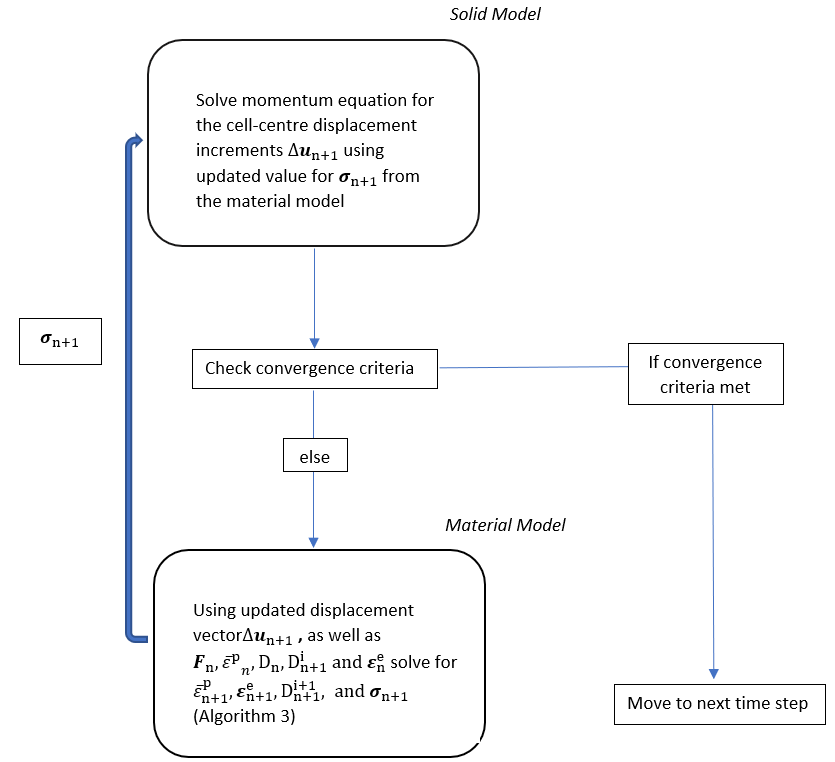
\includegraphics[width=0.9\textwidth]{./Figures/damageModels/lemaitreDamageSchematic.png}
%\caption{Schematic for overall algorithm}
%\label{fig:deforming body}
%\end{center}
%\end{figure}




%%\textbf{Implementation}
%%
%%Equation \ref{eqn:nonLocalEquation} is given in its strong integral form, with respect to the updated configuration, as
%%
%%\begin{equation}
%%\int_{\mathrm{\Omega}_u}D\ d\mathrm{\Omega}_u-\int_{\mathrm{\Omega}_u}\bar{D}\ d\mathrm{\Omega}_u+\oint_{\mathrm{\Gamma}_u}{{l_c}^2\ \mathbf{n}_u\cdot\mathrm{\nabla}\mathrm{\bar{D}}}\ d\mathrm{\Gamma}_u=0
%%\end{equation}
%%
%%In the context of the overall algorithm for the non-local Lemaitre damage model, the non-local damage $\bar{D}$ is solved for implicitly at the current iteration and the current time step, using the local damage $D$ at the current time step and current iteration.
%%
%%\begin{equation}
%%\int_{\mathrm{\Omega}_u}D^{i+1}^{[m+1]}\ d\mathrm{\Omega}_u-\int_{\mathrm{\Omega}_u}\bar{D}^{i+1}^{[m+1]}\ d\mathrm{\Omega}_u+\oint_{\mathrm{\Gamma}_u}{{l_c}^2\ \mathbf{n}_u\cdot\mathrm{\nabla}\mathrm{ \bar{D}^{i+1}^{[m+1]}}}\ d\mathrm{\Gamma}_u=0
%%\end{equation}
%
%\begin{algorithm}[H]
%\SetAlgoLined
%(i) Update Relative Deformation for given incremental displacement
%
%\begin{equation}
%  \mathbf{f}^{[m+1]}=\mathbf{I}+\nabla\left[\Delta\textbf{u}\right]\nonumber
%\end{equation}
%
%\begin{equation}
%\mathbf{F}^{[m+1]}=\mathbf{f}^{[m+1]}\mathbf{F}_n\nonumber
%\end{equation}
%(ii) Compute trial elasticity
%\begin{equation}
%\mathbf{B}^{e}^{[m]}=exp\left[{2\boldsymbol{\varepsilon}^{e}^{[m]}}\right]\nonumber
%\end{equation}
%\begin{equation}
%\mathbf{B}^{e}_{trial}=\mathbf{f}^{[m+1]}\mathbf{B}^{e}^{[m]}(\mathbf{f}^{[m+1]})^{T}\nonumber
%\end{equation}
%\begin{equation}
%\boldsymbol{\varepsilon}^{e}_{trial}=\frac{1}{2}ln[\textbf{B}^{e}_{trial}]\nonumber
%\end{equation}
%\begin{equation}
%\alpha_{trial}=\alpha^{[m]}\nonumber
%\end{equation}
%\begin{equation}
%\bar{\tau}_{eq}^{trial}=\sqrt{\frac{3}{2}}\lvert\lvert2\mu\ dev(\boldsymbol{\varepsilon}^{e}_{trial})\rvert\rvert\nonumber\nonumber
%\end{equation}
%\begin{equation}
%f_{trial}=  \bar{\tau}_{eq}^{trial}-\sigma_{y}(\alpha) \nonumber 
%\end{equation}
%  \eIf{$f_{trial}>0$}{
%   go to step iii to solve for $\Delta\gamma$
%   }{
%   $\Delta\gamma=0$ and go to step iv
%  }
%
%(iii) Enter small-strain return map and solve for $\Delta\gamma$ using the Newton-Raphson method to solve the equation:
%\begin{equation}
%\bar{\tau}_{eq}^{trial}-\frac{3\mu\Delta\gamma}{1-\bar{D}^{i}^{[m+1]}}-\sigma_{y}(a+\Delta\gamma)=0\nonumber
%\end{equation}
%(iv) Update Constitutive Variables
%\begin{equation}
%\alpha^{[m+1]}=\alpha_n+\Delta\gamma\nonumber
%\end{equation}
%\begin{equation}
%\boldsymbol{\varepsilon}^{e}^{[m+1]}=\boldsymbol{\varepsilon}^{e}_{trial}-\sqrt{\frac{3}{2}}\frac{\Delta\gamma}{\left(1-\bar{D}^{i}^{[m+1]}\right)}{\frac{dev(\boldsymbol{\varepsilon}^{e}_{trial})}{\lvert\lvert\boldsymbol{\varepsilon}^{e}_{trial}\rvert\rvert}}\nonumber
%\end{equation}
%\begin{equation}
%\boldsymbol{\tau}^{[m+1]}=\left(1-\bar{D}^{i}^{[m+1]}\right)\mathbf{D}^e:\boldsymbol{\varepsilon}^{e}^{[m+1]}\nonumber
%\end{equation}
%\begin{equation}
%\boldsymbol{\sigma}^{[m+1]}=\frac{1}{J}\boldsymbol{\tau}^{[m+1]}\nonumber
%\end{equation}
%(v) Update local damage field (equation \ref{DamageUpdateEquation})
%
%\ (vi) Update non-local damage field (equation \ref{eqn:nonLocalEquation})
%\caption{Non-local Lemaitre damage model}
%\end{algorithm}



%\subsubsection{Effective non-local damage development}
%
%
%One issue with the classic non-local Lemaitre damage model is that it can lead to a somewhat non-physical response. To illustrate this point, the results for the flat notched bar case with non-local Lemaitre damage (case a) and the notched round bar with non-local Lemaitre damage (case b) from the previous section are analysed. The cases looked at here use a time step of $0.001$ and a Rhie-Chow scale factor of $0.1$. The force-displacement curves and the damage evolution plotted at the cells where fracture first occurs (Figures \ref{axiMesh} and \ref{bordenMesh}) are given in Figures \ref{BordenNonLocalIssue} and \ref{AxiNonLocalIssue}.
%
%\begin{figure}[t!]
%	\centering
%		\subfigure[Force vs. displacement] {\label{airbus}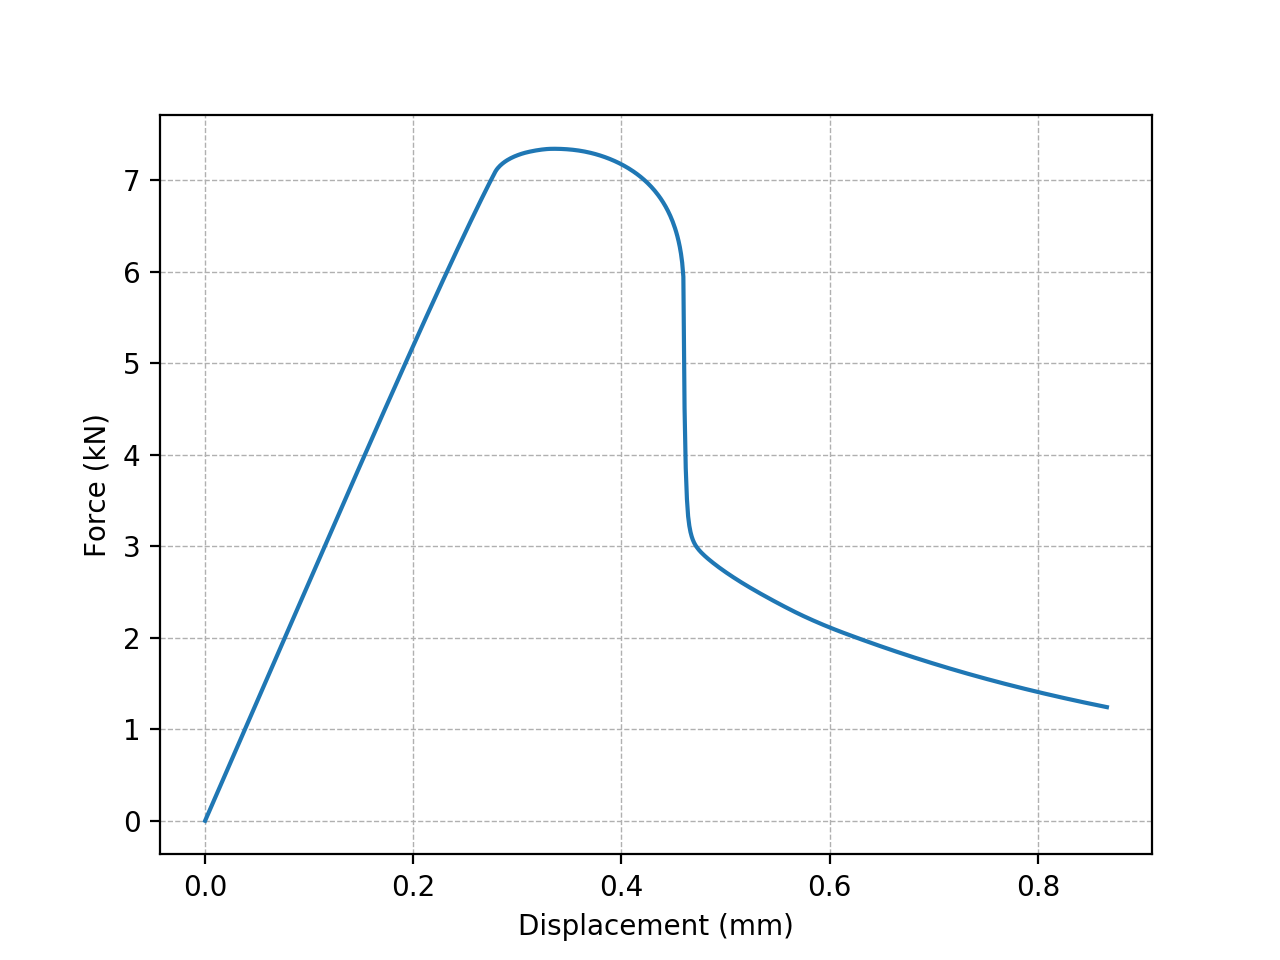
\includegraphics[width=0.45\textwidth]{./Figures/effectiveNonLocalDamage/CNLDispForceBorden.png}}
%		\qquad
%		\subfigure[non-local Damage vs. displacement] {\label{boeing} 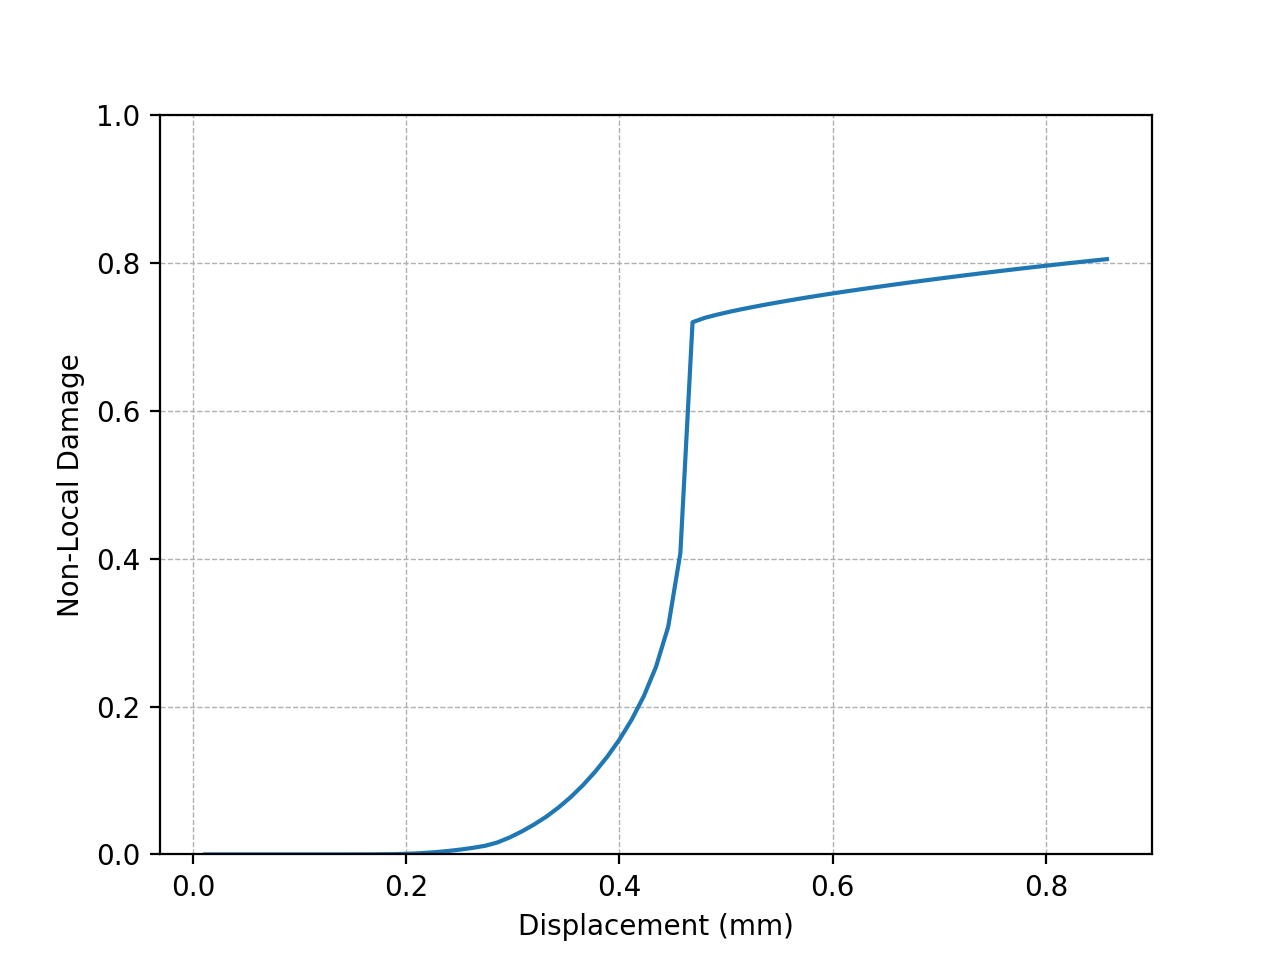
\includegraphics[width=0.45\textwidth]{./Figures/effectiveNonLocalDamage/disp_damageNonLocalBorden.png}}
%	\caption{Flat notched bar (case a)}
%	\label{BordenNonLocalIssue}
%\end{figure}
%\begin{figure}[t!]
%	\centering
%		\subfigure[Force vs. displacement] {\label{airbus}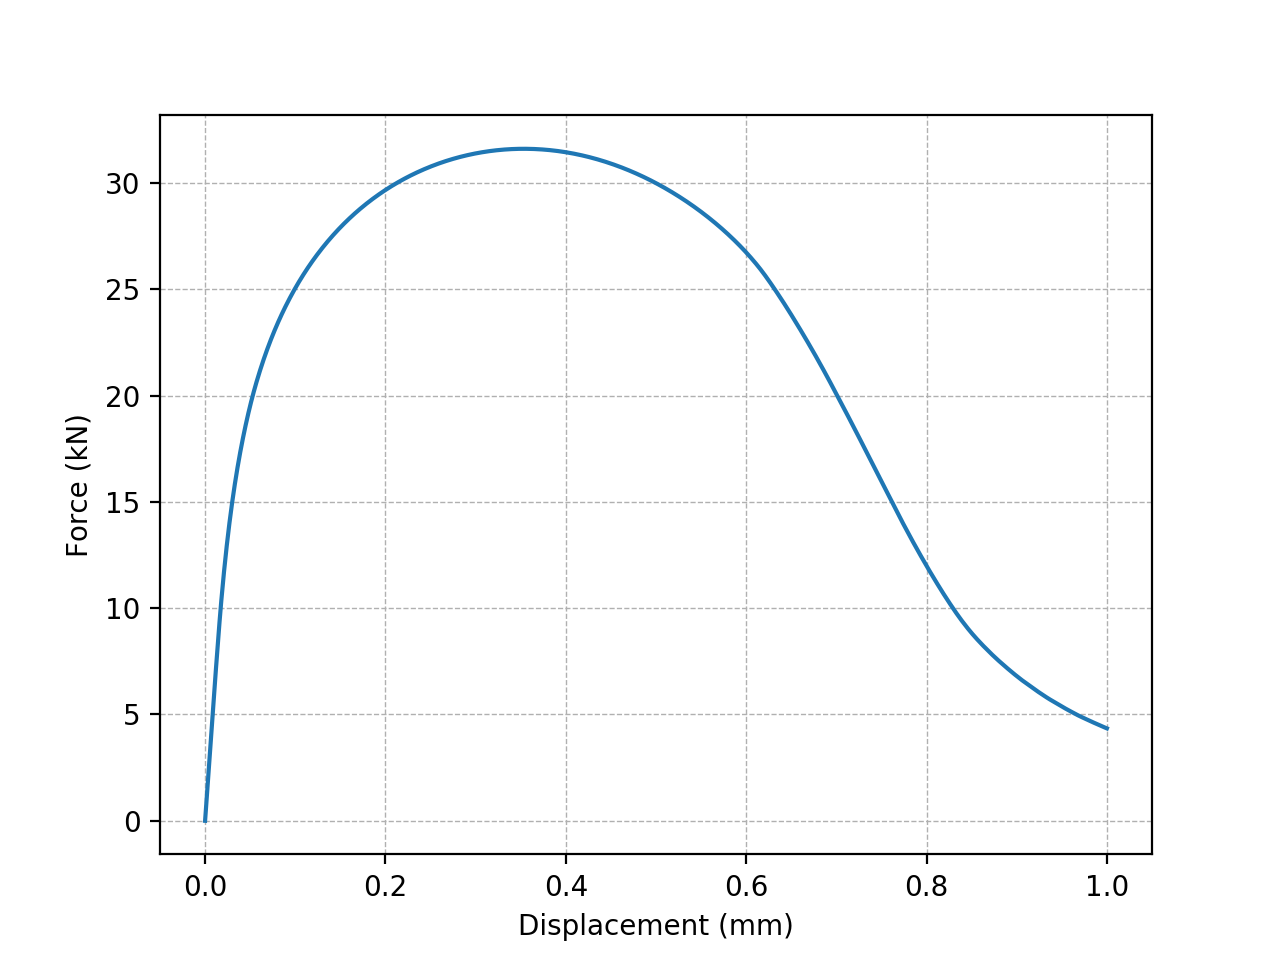
\includegraphics[width=0.45\textwidth]{./Figures/effectiveNonLocalDamage/CNLDispForceAxi.png}}
%		\qquad
%		\subfigure[non-local Damage vs. displacement] {\label{boeing} 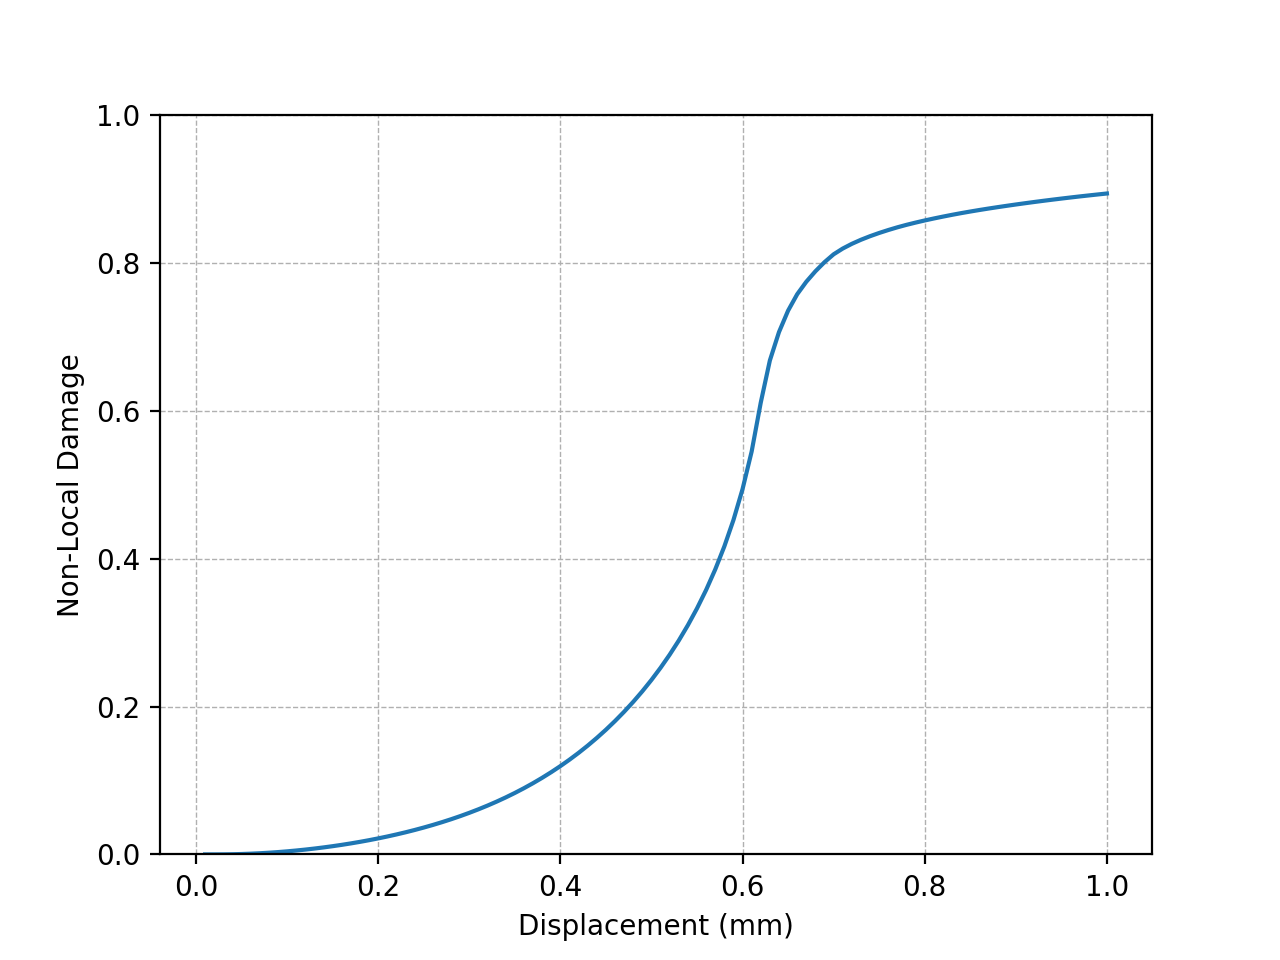
\includegraphics[width=0.45\textwidth]{./Figures/effectiveNonLocalDamage/disp_damageNonLocalAxi.png}}
%	\caption{Notched round bar (case b)}
%	\label{AxiNonLocalIssue}
%\end{figure}

Although subtle, we have found that limiting the value of the non-local damage field $\bar{D}$ (step (viii)) is critical for achieving reliable predictions.
%Non-physical issues with the damage evolution can be observed in Figures \ref{BordenNonLocalIssue} and \ref{AxiNonLocalIssue}. The non-local gradient equation has the effect of diffusing the damage such that after a certain point, the rate at which the damage evolves is reduced. In reality, it would be expected for the cell to quickly become fully damaged as it enters the void coalescence stage (Figure \ref{fig:Ductile-damage-evolution}) 
%To mitigate these issues, a novel formulation of the non-local Lemaitre model is developed in this work. The nonphysical response is mitigated by introducing the effective non-local damage field $\bar{D}_{eff}$. This field is set such that it is equivalent to the non-local damage field unless for a given cell the non-local damage field exceeds a critical damage value $D_c$. At this critical value, the effective non-local damage is set to be $0.99$. This cell can be viewed as essentially being fully degraded, the effective non-local damage $\bar{D}_{eff}$ is set as $0.99$ as opposed to $1.0$ in order to allow some small residual stresses in these cells to aid convergence.
%Further to this, the growth of the local damage for a given cell is prevented if the effective non-local damage of this cell exceeds the critical damage value $D_c$.
This step prevents nonphysical behaviour whereby a cell that is set as being fully damaged ($D = D_c$) is contributing to the damage growth in the surrounding cells through the non-local damage field.
%This scheme is described in Algorithm \ref{effectiveNonLocalDamage}.

%\begin{algorithm}[H]
%\label{effectiveNonLocalDamage}
%\SetAlgoLined
%(i) For all cells calculate local damage  \\
%
%  \eIf{$\bar{D}_{eff\ n+1}^{i} <= D_c$}{
%  \begin{equation}
%D^{i+1}^{[m+1]}=D_n+\frac{\Delta\gamma}{\left(1-D^{i}^{[m+1]}\right)}\left[\frac{-Y^{[m+1]}}{S_0}\right]^b \notag
%\end{equation} 
%   }{
%\begin{equation}
%D^{i+1}^{[m+1]}=D^{i}^{[m+1]} \notag
%\end{equation}
%  } 
%
%(ii) Calculate global non-local damage field
%\begin{equation}
%	\left(D^{i+1}^{[m+1]}-\bar{D}^{i+1}^{[m+1]}\right)+{{l_c}^2\mathrm{\nabla}}^2D^{i+1}^{[m+1]}=0 \notag	
%\end{equation}
%
%(iii) Set the effective non-local damage field for each cell \\
%\eIf{$\bar{D}^{[m+1]}^{i+1} <= D_c$}{
%\begin{equation}
%D^{i+1}_{eff\ n+1}=D^{i+1}^{[m+1]}\notag
%\end{equation} 
%   }{
%\begin{equation}
%D^{i+1}_{eff\ n+1}=0.99 \notag
%\end{equation}
%  } 
%\caption{Damage evolution scheme}
%\end{algorithm}







%%%%%%%%%%
\subsection{Gurson-Tvergaard-Needleman Model}
%%%%%%%%%%

\subsubsection{Model Formulation}

 \citet{gurson_continuum_1977} proposed the canonical micro-mechanical framework for ductile damage prediction and provides the basis for various derived models \cite{besson_continuum_2010, bettaieb_numerical_2011, achouri_numerical_2013m cao_models_2017, tekkaya_damage_2020}.
This model posits the existence of micro-voids in the material.
The density of these voids is described by a variable denoted as porosity.
The material degradation is characterised by the increasing porosity due to these voids' growth.
%Defining material degradation merely in terms of the growth of voids is limited, however.
Gurson’s framework was further developed by \citet{tvergaard_analysis_1984} to account for the void nucleation and coalescence, leading to the Gurson-Tvergaard-Needleman (GTN) model.
%To be consistent with how the GTN model is typically described in the literature \cite{bettaieb_numerical_2011,achouri_numerical_2013} and to present the equations in the form that they are implemented in the developed codes, the equivalent stress $\tau_{eq}$ is described using the symbol $q$ and the pressure $\tau_h$ is denoted by the symbol $p$. 

%\subsubsection{Evolution of Voids}

%The growth and nucleation of voids characterise the evolution of the porosity $f$:
%\begin{equation}
%	\dot{f}=\dot{f}_{growth}+\dot{f}_{nucleation}	
%\end{equation}	
%
%The growth of the voids is derived from the principle of mass conservation. It is given as a function of the strain rate:
%\begin{equation}
%	\dot{f}_{growth}=\left(1-f\right)tr\left(\dot{\boldsymbol{\varepsilon}}_p\right)	
%\end{equation}
% Where $\dot{\boldsymbol{\varepsilon}}_p$ is the plastic strain rate. 
%    
%The term for the nucleation of new voids is given by:
%\begin{equation}
%	{\dot{f}}_{nucleation}=A{\dot{\bar{\varepsilon}}}_p	
%\end{equation}
%
%
%Where ${\dot{\bar{\varepsilon}}}_p$ is the rate of change of the equivalent plastic strain and A is a dimensionless coefficient.
%The nucleation of new voids is assumed to be described by a normal distribution \cite{chu_void_1980} giving the following expression for the coefficient $A$:
%\begin{equation}
%\label{eqn:nucleatonA}
%A= \begin{cases}\frac{f_n}{S_n \sqrt{2 \pi}} \exp \left[-\frac{1}{2}\left(\frac{\bar{\varepsilon}_p-\varepsilon_n}{S_n}\right)\right] & \text { if } p>0 \\ 0 & \text { if } p<0\end{cases}
%\end{equation}
%
%where $f_n$ is the quantity of the voids nucleated per unit volume, $\varepsilon_n$ is the nucleation strain and $S_n$ is the standard deviation. 
%
%%\subsection{Yield equation}
%
%The variable f is coupled with the plasticity model through the yield equation 
%\begin{equation}
%	\phi=\left(\frac{q}{\sigma_y}\right)^2+2q_1f^\ast cosh\left(\frac{3q_2p}{2\sigma_y}\right)-\left(1-q_1^2f^{\ast2}\right)
%\end{equation}
%
%Where $q_1$ and $q_2$ are material parameters, $q$ is the von Mises stress, $p$ is the hydrostatic pressure and $\sigma_y$ is the yield stress.
%Here $f^\ast$ is the effective void fraction and is a function of the porosity variable defined above. It is introduced to account for the effects of void coalescence:
%\begin{equation}
%\label{eqn:GTNCoalescence}
%f^*=\left\{\begin{array}{cc}
%f & \text { if } f \leq f_c \\
%f_c+\left(f-f_c\right) \frac{f_u-f_c}{f_f-f_c} & \text { if } f>f_c
%\end{array}\right.
%\end{equation}
%
%Where $f_c$ is the void volume fraction at which the coalescence of voids begins,  $f_u$ is the ultimate volume fraction and $f_f$ represents the void volume fraction at fracture.
%
%%\subsection{Plasticity}
%
%Plastic isotropy and plastic associativity are assumed as in \citet{bettaieb_numerical_2011}. The following relation can therefore be obtained:
%\begin{equation}
%\label{eqn:4.67}
%	\dot{\boldsymbol{\varepsilon}}^p=\dot{\gamma}\frac{\partial\phi}{\partial\boldsymbol{\tau}}	
%\end{equation}
%
%This equation is reformulated in terms of the von Mises equivalent stress $q$ and the pressure $p$ to obtain:
%\begin{equation}
%	\label{eqn:4.68}
% \dot{\boldsymbol{\varepsilon}}^p=\dot{\gamma}\frac{\partial\phi}{\partial q}\frac{\partial q}{\partial\boldsymbol{\tau}}+\dot{\gamma}\frac{\partial\phi}{\partial p}\frac{\partial p}{\partial\boldsymbol{\tau}}
%\end{equation}
%
%Using the definitions of $q$ and $p$:
%\begin{equation}
%	\frac{\partial q}{\partial\boldsymbol{\tau}}=\mathbf{n}
% \end{equation}
% \begin{equation}
% \frac{\partial p}{\partial\boldsymbol{\tau}}=\frac{1}{3}\mathbf{I}	
%\end{equation}
%
%where $\mathbf{n}$ is given by:
%\begin{equation}
%\frac{3}{2q}\mathbf{\tau}_d.
%\end{equation}
%
%Equation \ref{eqn:4.68} can therefore be written as:
%\begin{equation}
%	\dot{\boldsymbol{\varepsilon}}^p=\dot{\gamma}\left(\frac{\partial\phi}{\partial q}\mathbf{n}+\frac{1}{3}\frac{\partial\phi}{\partial p}\mathbf{I}\right)	
%\end{equation}
%Which is equivalent to:
%\begin{equation}
%\label{eqn:4.73}
%\dot{\boldsymbol{\varepsilon}}^p=\frac{1}{3} \dot{\varepsilon}^h \boldsymbol{I}+\dot{\varepsilon}^q \boldsymbol{n}
%\end{equation}
%Where:
%\begin{equation}
%\label{eqn:4.74}
%\dot{ \boldsymbol{\varepsilon}}^h=\dot{\gamma} \frac{\partial \phi}{\partial p} 
%\end{equation}
%\begin{equation}
%\label{eqn:4.75}
%\dot{ \boldsymbol{\varepsilon}}^q=\dot{\gamma} \frac{\partial \phi}{\partial q}
%\end{equation}
%
%Eliminating $\dot{\gamma}$ from equations \ref{eqn:4.74}
%and \ref{eqn:4.75} leads to the consistency equation:
%\begin{equation}
%\dot{ \boldsymbol{\varepsilon}}^h \frac{\partial \phi}{\partial q}-\dot{ \boldsymbol{\varepsilon}}^q \frac{\partial \phi}{\partial p}=0
%\end{equation}
%
%
%%\subsection{Equivalent plastic strain}
%
%Assuming the equivalent plastic work principle, there is an equivalence between the rates of macroscopic and matrix plastic work:
%\begin{equation}
%\dot{\overline{\boldsymbol{\varepsilon}}}^p=\frac{\boldsymbol{\sigma}: \dot{\boldsymbol{\varepsilon}}^p}{(1-f) \sigma_y}
%\end{equation}
%Substituting in equation \ref{eqn:4.73}, the equation for the equivalent plastic strain is obtained in its final form:
%\begin{equation}
%\dot{\overline{\boldsymbol{\varepsilon}}}^p=\frac{p \dot{ \boldsymbol{\varepsilon}}^h+q \dot{\boldsymbol{\varepsilon}}^q}{(1-f) \sigma_y}
%\end{equation}
%
%%\subsection{Constitutive equations}
%\subsubsection{Model Formulation}

\hl{Andrew: check signs, assuming $p = -tr(\sigma)/3$}\\
\hl{Andrew: should $f$ be $f_*$ in the 2nd eqn?}\\
The GTN model is described by a yield equation, flow rule (deviatoric and volumetric), consistency condition, and porosity evolution equations:
\begin{eqnarray}
	&\Phi =
	\left(\frac{\sigma_v}{\sigma_y}\right)^2 + 2 q_1 f_* \cosh \left(\frac{3 q_2 p}{2 \sigma_y}\right)
	- \left(1-q_1^2 f^{2}_* \right) \label{eqn:GTN1} \\
	%= 0 \\
	&\dot{\bar{\varepsilon}}_p =
		\frac{1}{(1-f) \sigma_y} (\sigma_v \dot{ \bar{\varepsilon}}_\text{dev} - p \dot{ \bar{\varepsilon}}_\text{vol}) \label{eqn:GTN2} \\
	&\dot{\bar{\varepsilon}}_\text{vol} \frac{\partial \Phi}{\partial \sigma_v}
		+ \dot{\bar{\varepsilon}}_\text{dev} \frac{\partial \Phi}{\partial p} = 0 \label{eqn:GTN3} \\
	&\dot{f} = (1-f) \, \text{tr}\left(\dot{\boldsymbol{\varepsilon}}_p\right)+A \dot{\bar{\varepsilon}}_p \label{eqn:GTN4}
\end{eqnarray}
where $q_1$ and $q_2$ are material parameters.
The effective void fraction $f_*$, which accounts for void coalescence, is
\begin{equation} \label{eqn:GTNCoalescence}
	f_*=
	\left\{
	\begin{array}{cc}
		f & \text { if } f \leq f_c \\
		f_c+\left(f-f_c\right) \frac{f_u-f_c}{f_f-f_c} & \text { if } f>f_c
	\end{array}\right.
\end{equation}
where $f$ is the porosity, $f_c$ is the void volume fraction at which void coalescence begins, $f_u$ is the ultimate volume fraction, and $f_f$ is the volume fraction at fracture.

The rate of volumetric plastic strain and equivalent deviatoric plastic strain are given, respectively, by
\begin{eqnarray}
	\dot{ \boldsymbol{\varepsilon}}_\text{vol} &=& \dot{\bar{\varepsilon}}_p \frac{\partial \phi}{\partial p} \\
	\dot{ \boldsymbol{\varepsilon}}_\text{dev} &=& \dot{\bar{\varepsilon}}_p \frac{\partial \phi}{\partial \sigma_v}
\end{eqnarray}


%Where ${\dot{\bar{\varepsilon}}}_p$ is the rate of change of the equivalent plastic strain and 
The dimensionless coefficient $A$ is chosen to ensure void nucleation follows a normal distribution \cite{chu_void_1980}:
\begin{equation} \label{eqn:nucleatonA}
	A =
	\begin{cases}
	\frac{f_n}{S_n \sqrt{2 \pi}} \exp \left[-\frac{1}{2}\left(\frac{\bar{\varepsilon}_p-\varepsilon_n}{S_n}\right)\right] & \text { if } p < 0 \\
	0 & \text { if } p \geq 0
	\end{cases}
\end{equation}
where $f_n$ is the quantity of the voids nucleated per unit volume, $\varepsilon_n$ is the nucleation strain and $S_n$ is the standard deviation. 



%\paragraph{Shear Effects}
\paragraph{Lode Angle Dependence}

Further developments of the GTN model have been made to better account for fracture in stress states with significant shearing \cite{nahshon_modification_2008, malcher_continuum_2012, leclerc_micromechanics-based_2020, achouri_numerical_2013}.
This work adopts the expression developed by \citet{nahshon_modification_2008} for shearing-related void growth, which has shown an ability to accurately predict fracture in the blanking metal forming process \cite{achouri_numerical_2013}.
The porosity evolution equation (Equation \label{eqn:GTN4}) is consequently replaced by
%\begin{equation}
%	\dot{f}={\dot{f}}_{growth}+{\dot{f}}_{nucleation}+{\dot{f}}_{shear}	
%\end{equation}
where
\begin{equation}
%	{\dot{f}}_{shear}=k_w\frac{fw\left(\boldsymbol{\sigma}\right)}{q}\mathbf{s}:{\dot{\boldsymbol{\varepsilon}}}_p	
	\dot{f} = (1-f) \, \text{tr}\left(\dot{\boldsymbol{\varepsilon}}_p\right)+A \dot{\bar{\varepsilon}}_p
%	+ k_w\frac{fw\left(\boldsymbol{\sigma}\right)}{q}\mathbf{s}:{\dot{\boldsymbol{\varepsilon}}}_p
	+ k_w f\frac{1 - \xi^2 }{\sigma_v} \,\text{dev}(\bb{\sigma}):{\dot{\boldsymbol{\varepsilon}}}_p
\end{equation}
%where $k_w$ is a material parameter and $w(\boldsymbol{\sigma})$ is given by
%\begin{equation}
%	w\left(\boldsymbol{\sigma}\right) = 1- \xi^2	
%\end{equation}


\paragraph{Non-Local Porosity}

Like the Lemaitre model, mesh dependency in the GTN model can be mitigated by introducing non-local damage variables \cite{reusch_non-local_2003, leclerc_micromechanics-based_2020}.
In the case of the GTN model, a non-local porosity variable is determined using a non-local gradient (smoothing) equation:
\begin{equation}
	\bar{f} - {l_c}^2 \bb{\nabla}^2 \bar{f} = f
\end{equation}
where $\bar{f}$ is the non-local (smoothed) porosity field.
This equation can be discretised, as before, using the described cell-centred finite volume method and zero-flux Neumann boundary conditions.
%  The effective porosity $f^\ast$ is then calculated according to equation \ref{eqn:GTNCoalescence} using the non-local porosity $\bar{f}$. Where $f$ appears in the system of equations \ref{eqn:discritesedGTNSystem} the non-local porosity is used.



\subsubsection{Computational Procedure}

\hl{Philip reminder: make notation consistent for tensor multiplication}\\
For the GTN model, the elastoplasticity stress calculation is extended to determine porosity $f$ in addition to stress and plastic strain.
The adopted computational algorithm is shown in Algorithm \ref{alg:GTN}.
As in the Lemaitre computational procedure, we propose an explicit-implicit algorithm to solve the system of equations:
Equations \ref{eqn:GTN1}, \ref{eqn:GTN2} and \ref{eqn:GTN3} are solved implicitly for the variables $\boldsymbol{\varepsilon}_\text{vol}$, $\boldsymbol{\varepsilon}_\text{dev}$ and $\overline{\boldsymbol{\varepsilon}}_p$ using a Newon-Raphson method, while the porosity $f$ (Equation \ref{eqn:GTN4}) is calculated in a deferred-correction/explicit manner.
Once again, the overall procedure is implicit in time.

%For each cell, the incremental displacement field $\Delta\mathbf{u}$ for the current time step, at the current iteration, is given. The values of the following variables from the previous time step are also provided:
%\begin{equation}
%\left\{F_n^p,\ {{\bar{\varepsilon}}^p}_n,f_n\right\}
%\end{equation}
%The goal is then to have a computational procedure to obtain the following variables at time $t^{[m+1]}$
%\begin{equation}
%\left\{F^{[m+1]}^p,\ {{\bar{\varepsilon}}^p}^{[m+1]},\boldsymbol{\sigma}^{[m+1]},f^{[m+1]}\right\}
%\end{equation}
%This is achieved in the material solver by solving the set of equations laid out in equation \ref{eqn:4.79}.
%
%Equation 3.30 is given in terms of the GTN yield equation:
%\begin{equation}
%	{\dot{\mathbf{F}}}^p\mathbf{F}^{p-1}=\Delta\gamma\mathbf{R}^{eT}\frac{\partial\phi}{\partial\boldsymbol{\tau}}\mathbf{R}^e
%\end{equation}
%Employing the exponential map backward scheme for the time-discretisation of the plastic flow rule, one can obtain:
%\begin{equation}
%	\mathbf{F}^{[m+1]}^p=exp\left[\Delta\gamma\mathbf{R}^{[m+1]}^{e^T}\frac{\partial\phi}{\partial\boldsymbol{\tau}^{[m+1]}}\mathbf{R}^{[m+1]}^e\right]\mathbf{F}_n^p
%\end{equation}
%Due to plastic isotropy this equation can be written as:
%\begin{equation}
%	\mathbf{F}^{[m+1]}^p=\mathbf{R}^{[m+1]}^{e^T}exp\left[\Delta\gamma\frac{\partial\phi}{\partial\boldsymbol{\tau}^{[m+1]}}\right]\mathbf{R}^{[m+1]}^e\mathbf{F}_n^p
%\end{equation}
%Subbing in equation \ref{eqn:4.67}
%\begin{equation}	\mathbf{F}^{[m+1]}^p=\mathbf{R}^{[m+1]}^{e^T}exp\left[\Delta{\boldsymbol{\varepsilon}}^p^{[m+1]}\right]\mathbf{R}^{[m+1]}^e\mathbf{F}_n^p	
%\end{equation}
%Using the same procedure laid out in section 3.2.3, the additive split for the elastic and plastic contributions is obtained:
%\begin{equation}
%\boldsymbol{\varepsilon}^{[m+1]}^e=\boldsymbol{\varepsilon}^{[m+1]}^{e \text { trial }}-\Delta \varepsilon^{[m+1]}^p
%\end{equation}

%The porosity $f^{[m+1]}$ is then solved for explicitly. 
%Using the fact that:
%\begin{equation}
%p^{[m+1]}=p_{\text {trial }}-K \Delta \varepsilon^{[m+1]}^h 
%\end{equation}
%\begin{equation}
%q^{[m+1]}=q_{\text {trial }}-3 \mu \Delta \varepsilon^{[m+1]}^q
%\end{equation}


%The system of equations to be solved, $r_i$, implicitly are given by
%\begin{equation}
%\label{eqn:discritesedGTNSystem}
%\left\{\begin{array}{c}
%r_{\Delta \varepsilon^{[m+1]}^q}=\left(\frac{q_{\text {trial }}-3 \mu \Delta \varepsilon^{[m+1]}^q}{\sigma_y\left(\bar{\varepsilon}^p+\Delta \bar{\varepsilon}^p{ }^{[m+1]}\right)}\right)^2+2 q_1 f^{*i}^{[m+1]} \cosh \left(\frac{3 q_2\left(p_{\text {trial }}-K \Delta \varepsilon^{[m+1]}^h\right)}{2 \sigma_y\left(\bar{\varepsilon}^p+\Delta \bar{\varepsilon}^p{ }^{[m+1]}\right)}\right)-\left(1-q_1^2 {f^{*i}}^2^{[m+1]}\right)=0 \\
%r_{\Delta \varepsilon^{[m+1]}^h}=\Delta \varepsilon^{[m+1]}^h \frac{\partial \phi}{\partial q}-\Delta \varepsilon^{[m+1]}^q \frac{\partial \phi}{\partial p}=0 \\
%r_{\Delta \bar{\varepsilon}^p{ }^{[m+1]}}=\Delta \bar{\varepsilon}^p{ }^{[m+1]}-\frac{p \Delta \varepsilon^{[m+1]}^h+q \Delta \varepsilon^{[m+1]}^q}{(1-f^i^{[m+1]}) \sigma_y\left(\bar{\varepsilon}^p+\Delta \bar{\varepsilon}^p{ }^{[m+1]}\right)}=0
%\end{array}\right.
%\end{equation}
%The group of unknowns associated with this system of equations is given by $x_i$
%\begin{equation}
%x_i=\left\{\begin{array}{c}
%\Delta \varepsilon^{[m+1]}^q \\
%\Delta \varepsilon^{[m+1]}^h \\
%\Delta \bar{\varepsilon}^p
%\end{array}\right\}
%\end{equation}
%The system of equations is solved at the centre of each volume using the Newton-Raphson method
%\begin{equation}
%\boldsymbol{x}_{i n+1}=\boldsymbol{x}_{i n}-\left[\left.\frac{\partial \boldsymbol{r}_i}{\partial \boldsymbol{x}_i}\right|_{\boldsymbol{x}_n}\right]^{-1} \boldsymbol{r}_i\left(\boldsymbol{x}_n\right)
%\end{equation}
%$\frac{\partial r_i}{\partial x_i}$ is the Jacobian of the equations $r_i$ with respect to the variables $x_i$ given by:
%\begin{equation}
%\frac{\partial \boldsymbol{r}_i}{\partial \boldsymbol{x}_i}=\left[\begin{array}{ccc}
%\frac{\partial r_{\Delta \varepsilon^{[m+1]}^q}^q}{\partial \Delta \boldsymbol{\varepsilon}^{[m+1]}^q} & \frac{\partial r_{\Delta \varepsilon^{[m+1]}^q}^q}{\partial \Delta \boldsymbol{\varepsilon}^{[m+1]}^h} & \frac{\partial r_{\Delta \varepsilon^{[m+1]}^q}^q}{\partial \Delta \overline{\boldsymbol{\varepsilon}}^p^{[m+1]}} \\
%\frac{\partial r_{\Delta \varepsilon^{[m+1]}^h}}{\partial \Delta \boldsymbol{\varepsilon}^{[m+1]}^q} & \frac{\partial r_{\Delta \varepsilon^{[m+1]}^h}}{\partial \Delta \boldsymbol{\varepsilon}^{[m+1]}^h} & \frac{\partial r_{\Delta \varepsilon^{[m+1]}^h}}{\partial \Delta \overline{\boldsymbol{\varepsilon}}^p{ }^{[m+1]}} \\
%\frac{\partial r_{\Delta \overline{\boldsymbol{\varepsilon}}^p{ }^{[m+1]}}}{\partial \Delta \boldsymbol{\varepsilon}^{[m+1]}^q} & \frac{\partial r_{\Delta \overline{\boldsymbol{\varepsilon}}^p{ }^{[m+1]}}}{\partial \Delta \boldsymbol{\varepsilon}^{[m+1]}^h} & \frac{\partial r_{\Delta \overline{\boldsymbol{\varepsilon}}^p{ }^{[m+1]}}}{\partial \Delta \overline{\boldsymbol{\varepsilon}}^p{ }^{[m+1]}}
%\end{array}\right]
%\end{equation}
%Using simple multivariable calculus operations these constituent partial derivatives of the Jacobian can then be derived. These derivatives are provided in Appendix C **. 
%After solving for these variables
%($\Delta {\varepsilon}^{[m+1]}^h$, $\Delta {\varepsilon}^{[m+1]}^q$ and $\Delta \overline{{\varepsilon}}^p$) the equivalent plastic strain, elastic strain, pressure, von Mises stress and stress can then be updated:
%\begin{equation}
%\vec{\varepsilon}^p{ }^{[m+1]}=\vec{\varepsilon}^p{ }_n+\Delta \vec{\varepsilon}^p{ }^{[m+1]} 
%\end{equation}
%\begin{equation}
%\boldsymbol{\varepsilon}^{e}^{[m+1]}=\boldsymbol{\varepsilon}^{e}_{trial}-\frac{1}{3}\Delta {\varepsilon}^{[m+1]}^h\ \mathbf{I}-\Delta {\varepsilon}^{[m+1]}^q\ \mathbf{n}
%\end{equation}
%\begin{equation}
%p^{[m+1]}=p_{\text {trial }}-K \Delta \varepsilon^{[m+1]}^h 
%\end{equation}
%\begin{equation}
%q^{[m+1]}=q_{\text {trial }}-3 \mu \Delta \varepsilon^{[m+1]}^q 
%\end{equation}
%\begin{equation}
%\boldsymbol{\tau}^{[m+1]}=p^{[m+1]} \boldsymbol{I}+\frac{2q^{[m+1]}}{3} \boldsymbol{n} 
%\end{equation}
%The porosity can then be determined:
%\begin{equation}
%f_{\mathrm{n}+1}^{\mathrm{i}+1}=f_{\mathrm{n}}+\left(1-f_{\mathrm{n}+1}^{\mathrm{i}}\right) \operatorname{tr}\left(\Delta \varepsilon^{[m+1]}^p\right)+A \Delta \bar{\varepsilon}^p{ }^{[m+1]}
%\end{equation}

%Where ${f}^{[m+1]}^{i+1}$ is the porosity for the current iteration and $f^{[m+1]}^i$ is the porosity from the previous iteration. The effective porosity $f^{*i+1}^{[m+1]}$ is then calculated according to equation \ref{eqn:GTNCoalescence}.
%This procedure is provided in Algorithm 5.

\begin{algorithm}[htbp] \label{alg:GTN} \footnotesize
\SetAlgoLined
(i) Update deformation gradients for a given incremental displacement

\begin{equation}
  \textbf{f}^{[m+1]}=\textbf{I}+\nabla\left[\Delta\textbf{u}\right]^T \nonumber
\end{equation}
\begin{equation}
 \textbf{F}^{[m+1]}=\textbf{f}^{[m+1]}\textbf{F}_n\nonumber
\end{equation}

(ii) Compute trial elastic state
\begin{equation}
	\mathbf{B}_{e}^{[m]} = \exp\left({2\boldsymbol{\varepsilon}_{e}^{[m]}}\right) \nonumber
\end{equation}
\begin{equation}
\mathbf{B}^{\text{trial}}_e =\mathbf{f}^{[m+1]}\mathbf{B}_{e}^{[m]}(\mathbf{f}^{[m+1]})^{T}\nonumber
\end{equation}
\begin{equation}
\boldsymbol{\varepsilon}_e^{\text{trial}}=\frac{1}{2} \ln[\textbf{B}^{\text{trial}}_e]\nonumber
\end{equation}
%\begin{equation} % Philip: what is this used for?
%\bar{\varepsilon}^{p}_{\text{trial}}=\bar{\varepsilon}_{p}^{[m]}\nonumber
%\end{equation}
\begin{equation}
	p^{\text{trial}} = \kappa \, \text{tr}(\boldsymbol{\varepsilon}_{e}^{\text{trial}})\nonumber
\end{equation}
\begin{equation}
	\mathbf{s}^{\text{trial}}=2 \mu \, \text{dev}(\boldsymbol{\varepsilon}_{e}^{\text{trial}})\nonumber
\end{equation}
\begin{equation}
	\sigma^{\text{trial}}_v = \sqrt{\sfrac{3}{2}} ||  2\mu \, \text{dev}(\boldsymbol{\varepsilon}^{e}_{\text{trial}})|| \nonumber
\end{equation}
\begin{equation}
    \mathbf{n}=\frac{3}{2}\frac{\mathbf{s}^{\text{\text{trial}}}}{\sigma_v^{\text{trial}}}\nonumber
\end{equation}
\begin{equation}
	\Phi^{\text{trial}} = 
	\left(\frac{\sigma_v^{\text{trial}}}{\sigma_{y}}\right)^{2}
	+ q_{1}f_{*[i]}^{[m+1]} \cosh\left(\frac{3q_{2}p^{\text{trial}}}{2\sigma_{y}}\right)
	-\left(1-q_{1}^{2}{f_{*[i]}^{[m+1]}}^2\right)\nonumber
\end{equation}
  \eIf{$\Phi^{\text{trial}}>0$}{
   go to step (iii)
   }{
   set $\Delta \varepsilon_\text{vol} = \Delta \varepsilon_\text{dev} = \Delta \bar{\varepsilon}_p = 0$ and $\Delta \bb{\varepsilon}_p = \bb{0}$. Go to step (iv)
  }

(iii) Enter small strain return map and solve the system of equations (equation \ref{eqn:discritesedGTNSystem}) for $\Delta {\varepsilon}^{[m+1]}_h$, $\Delta {\varepsilon}^{[m+1]}_q$ and $\Delta \overline{{\varepsilon}}^p_{[m+1]}$


(iv) Update the constitutive variables
\begin{equation}
	\bar{\varepsilon}_p^{[m+1]} = \bar{\varepsilon}_p^{[m]} + \Delta \bar{\varepsilon}_p \nonumber
\end{equation}
\begin{equation}
	\bb{\varepsilon}_p^{[m+1]} = \bb{\varepsilon}_p^{[m]} +\Delta \bb{\varepsilon}_p \nonumber
\end{equation}
\begin{equation}
	\boldsymbol{\varepsilon}_{e}^{[m+1]} = \boldsymbol{\varepsilon}^{\text{trial}}
	- (\sfrac{1}{3}) \Delta {\varepsilon}^{[m+1]}_\text{vol} \, \mathbf{I}
	- \Delta {\varepsilon}^{[m+1]}_\text{dev} \, \mathbf{n}\nonumber
\end{equation}
\begin{equation}
	\boldsymbol{s}^{[m+1]} =
	\frac{1}{J}
	\left[
%	 	\left(
%			p_{\text {trial }} - \kappa \Delta \varepsilon^{[m+1]}_{\text{vol}}
%		\right)\mathbf{I}
%		+
		\sfrac{2}{3} \left(\sigma_v^{\text {trial }} - 3 \mu \Delta \varepsilon^{[m+1]}_\text{dev} \right) \mathbf{n}
	\right] \nonumber
\end{equation}
%\begin{equation}
%\boldsybol{\tau}^{[m+1]}=\left(q_{trial}-3\mu\Delta \boldsymbol{\varepsilon}^{[m+1]}^q\left(\frac{3\mathbf{s}_{trial}}{2q_{trial}}\right)\right)+\left(p_{trial}-K\Delta\varepsilon^{h}^{[m+1]}\right)\nonumber
%\end{equation}

%\begin{equation}
%\boldsymbol{\sigma}^{[m+1]}=\frac{1}{J}\boldsymbol{\tau}^{[m+1]}\nonumber
%\end{equation}

(v) Implicitly solve the pressure Poisson's equation:
\begin{equation}
	p^{[m+1]} - \mathbb{D} \bb{\nabla}^2 p^{[m+1]} =
%	-\frac{\kappa}{2} \left[\left(J^{[m+1]}\right)^{2} - 1\right]
	\frac{1}{J}\left(p_{\text {trial }} - \kappa \Delta \varepsilon^{[m+1]}_{\text{vol}} \right)
	- \bb{\nabla} \cdot \left( \mathbb{D} \bb{\nabla} p^{[m+1]}_{[i]} \right) \\
\end{equation}


(vi) Update the true (Cauchy) stress
\begin{equation}
	\boldsymbol{\sigma}^{[m+1]} = \boldsymbol{s}^{[m+1]} -  p^{[m+1]}\textbf{I} \nonumber
\end{equation}


(vii) Calculate the porosity $f_{[i+1]}^{[m+1]}$ and the effective porosity $f_{*[i+1]}^{[m+1]}$:
\begin{equation}
	f^{[m+1]} = f^{[m]} + \left(1 - f^{[m+1]}_{[i]}\right) \, \text{tr}\left(\dot{\boldsymbol{\varepsilon}}^{[m+1]}_p\right)
	+ A \dot{\bar{\varepsilon}}^{[m+1]}_p
	+ k_w f\frac{1 - \xi^2 }{\sigma_v^{[m+1]}} \,\text{dev}(\bb{\sigma}^{[m+1]}):{\dot{\boldsymbol{\varepsilon}}}_p^{[m+1]}
\end{equation}
\begin{equation}
	f^{*[m+1]} =
	\left\{
	\begin{array}{ll}
		f^{[m+1]}  & \text { if } f^{[m+1]}  \leq f_c \\
		f_c + \left(f^{[m+1]} - f_c\right) \frac{f_u - f_c}{f_f - f_c} & \text { if } f^{[m+1]}  > f_c
	\end{array}\right.
\end{equation}


(viii) Implicitly solve non-local porosity equation:
\begin{equation}
	\bar{f}^{[m+1]} -  l_c^2 \bb{\nabla}^2 \bar{f}^{[m+1]} = f^{[m+1]}
\end{equation}

\caption{GTN damage model stress calculation algorithm}
\end{algorithm}






\subsection{Phase field fracture model}

\subsubsection{Model Formulation}
In recent years, phase field approaches have received much attention for the prediction of fracture and failure \cite{borden_phase-field_2012, miehe_phase_2010, ambati_phase-field_2015, borden_phase-field_2016, miehe_phase_2016, dittmann_variational_2018, samaniego_phase-field_2021}, showing an ability to predict complex crack patterns, including branching and merging in both two and three dimensions \cite{borden_phase-field_2012, miehe_phase_2010}.
In this method, sharp cracks are \emph{regularised} over a continuum, leading to a system of partial differential equations that are relatively simple to implement in finite element, finite volume and related solvers.
%The method has proven robust with computations being performed on the original mesh without any need to track the interface of the crack such as in the Cohesive-zone model method.

The phase field method for damage, initially proposed by \citet{francfort_revisiting_1998} to describe brittle fracture, is based on a variational approach to minimise a Griffiths theory potential energy functional. %proposed based on Griffiths theory of brittle fracture.
This approach leads to a Mumford-Shah \cite{mumford_optimal_1989} type energy potential that can be approximated by a phase-field formulation following the work of \citet{ambrosio_approximation_1990}.
This approximation was adopted by \citet{bourdin_time-discrete_2011} to facilitate numerical solutions of the variational formulation, and further extended by \citet{miehe_phase_2010} who derived the phase field approach from continuum mechanics and thermodynamic arguments.
%In addition to an alternative derivation,
\citet{miehe_phase_2010} also added an important mechanism for distinguishing between tensile and compressive effects on crack growth, as well as including a history variable $\mathcal{H}$ which ensures the irreversibility of crack growth.
Several studies have shown the ability of these models to produce results consistent with benchmark fracture cases \cite{borden_phase-field_2012,miehe_phase_2010}.

The phase field approach has since been extended to ductile fracture by \citet{ambati_phase-field_2015, borden_phase-field_2016} and \citet{miehe_phase_2016}.
The approach from \citet{ambati_phase-field_2015} involves incorporating a plastic strain dependency in the elastic degradation function while the approach from \citet{miehe_phase_2016} incorporates the plastic strain energy into the crack driving variable $\mathcal{H}$.
\citet{borden_phase-field_2016} uses a similar approach to \citet{miehe_phase_2016} by incorporating the plastic strain into the crack driving variable $\mathcal{H}$ while also introducing a plastic degradation function to ensure that fracture is preceded by large plastic strains, as is the case experimentally.



%%%%%%%%%%%%%%%%
%\subsection{Phase Field Damage Model}
%%%%%%%%%%%%%%%%
%
%The original formulation of the potential energy of the body \cite{mumford_optimal_1989} is given in terms of the deformation tensor and the crack surface
%\begin{equation}
%\label{eqn:originalPotentialEnergyFormulation}
%	E\left(\boldsymbol{\varepsilon}^e,\Gamma_0\right)=\int_{\Omega_0}{\psi\left(\boldsymbol{\varepsilon}^e\right)d\Omega_0}+\int_{\Gamma_0}{G_c^0\ d\Gamma_0}
%\end{equation}
%Where $\psi\left(\boldsymbol{\varepsilon}^e\right)$ is the elastic contribution to the potential energy per unit volume and $G_c$ is the critical fracture energy per unit area. This energy functional is an extension of Griffith’s definition of brittle fracture. This definition of the fracture surface however requires an a priori determination of the fracture surface. In order to enable an efficient numerical treatment of equation \ref{eqn:originalPotentialEnergyFormulation}, \citet{bourdin_time-discrete_2011} introduced the phase field approximation: 
%\begin{equation}
%	E\left(\boldsymbol{\varepsilon}^e,\Gamma_0\right)=\int_{\Omega_0}{g_e(d)\psi\left(\boldsymbol{\varepsilon^e}\right)d\Omega_0}+\int_{\Gamma_0}{G_c^0\ \Gamma_l\left(d\right)d\Omega_0}
%\end{equation}
%
%where $d\left(x\right)\in\left[0,1\right]$,  $d=0$ characterises the unbroken state and d=1 characterises the fully broken state. The variable $d$ is conceptually similar to the damage variable $D$ used in continuum damage mechanics, with $d$ being a macroscopic variable that characterizes the growth of micro voids and micro-cracks, $g_e(d)$ is the elastic degradation function which reduces the elastic strength of the material and $\Gamma_l$ is the crack density functional, which for the model of \citet{borden_phase-field_2016} is given by
%
%\begin{equation}
%	\Gamma_l\left(d\right)=\frac{1}{l}I\left(d\right)=\frac{1}{4l}\left(d^2+4l^2|\nabla d|\right)
%\end{equation}
%The minimization of this functional gives the regularised crack surface as depicted in Figure \ref{fig:Regularising effects of l}. The parameter $l$ is a length scale variable which regularises the crack surface.
%
%% \begin{figure}[t!]
%%	\centering
%%		\subfigure[] {\label{airbus}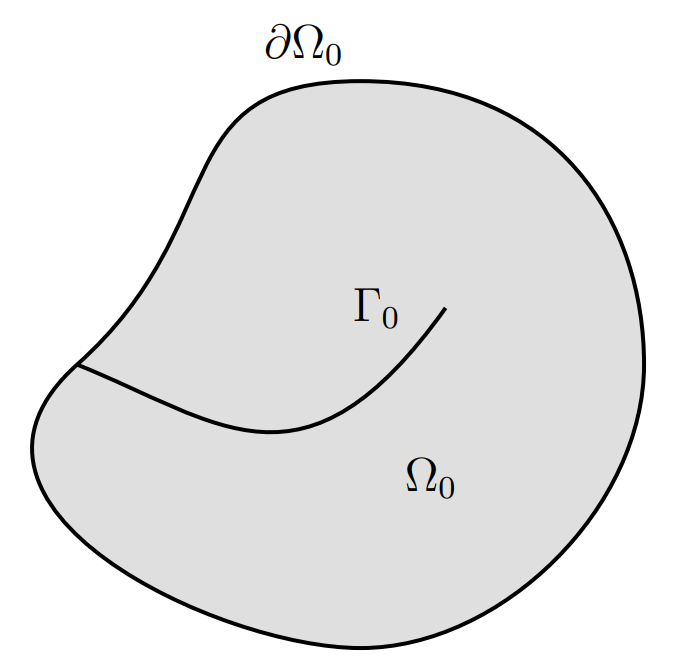
\includegraphics[width=0.3\textwidth]{./Figures/damageModels/phaseSharpCrack.png}}		
%%	  \qquad
%%		\subfigure[] {\label{boeing} 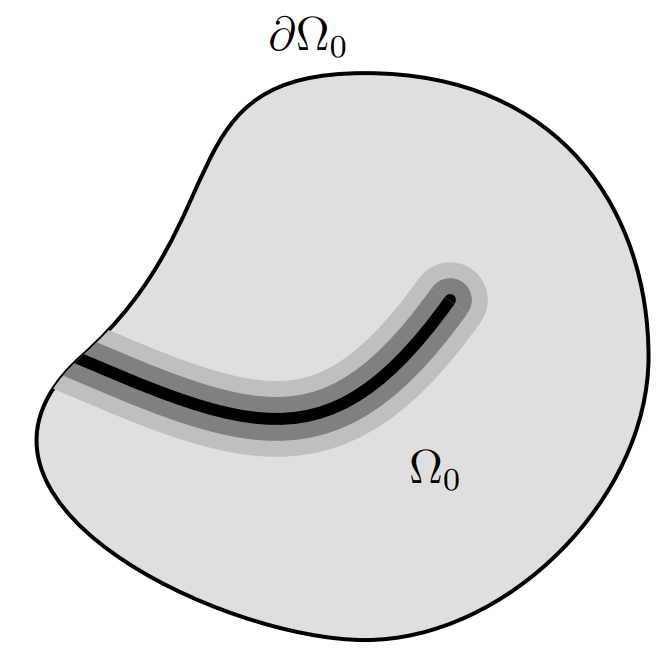
\includegraphics[width=0.3\textwidth]{./Figures/damageModels/phaseRegularised.png}}		
%%\caption{Comparison of a) sharp crack and b) diffusive crack (adapted from \cite{borden_phase-field_2016})}
%%	\label{fig:diffusedSharpCrack}
%%\end{figure}
%%\FloatBarrier
%%
%%\begin{figure}[htb]
%%\begin{center}
%%	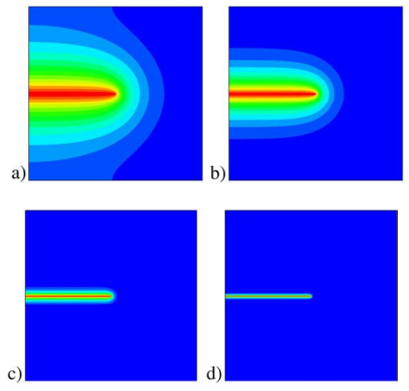
\includegraphics[width=0.65\textwidth]{./Figures/damageModels/effectsofl.png}
%%\caption{Illustration of the regularising effect of $l$, as $l$ is reduced the crack variable $d$ is regularised over a smaller area}
%%\label{fig:Regularising effects of l}
%%\end{center}
%%\end{figure}
%%\FloatBarrier
%
%As in \citet{amor_regularized_2009,miehe_phase_2010-1} the elastic strain energy contribution is further split into its tensile and compressive contribution, to ensure that there is no elastic contribution to crack growth when a given volume is under compression
%\begin{equation}
%\label{eqn:energyElasticFunctional}
%E_l\left(\mathbf{\boldsymbol{\varepsilon}^e},d\right)=\int_{\Omega_0}\left(g_e\left(d\right){\psi_e}^+\left(\boldsymbol{\varepsilon}^e\right)+g_e\left(d\right){\psi_e}^-\left(\boldsymbol{\varepsilon}^e\right)\right)\ d\Omega_0+\int_{\Gamma_0}{G_c^0\Gamma_l\left(d\right)\Omega_0}	
%\end{equation}
%
%Where ${\psi_e}^+\left(\boldsymbol{\varepsilon}^e\right)$ is the contribution of the tensile strains and ${\psi_e}^-\left(\boldsymbol{\varepsilon}^e\right)$ is the contribution of the compressive strains. The energy functional in equation \ref{eqn:energyElasticFunctional} only accounts for the elastic contribution to crack growth. For ductile materials, it is necessary to incorporate a plastic energy contribution to the crack growth. To this end, a plastic energy contribution is added to equation \ref{eqn:energyElasticFunctional} in \citet{borden_phase-field_2016}
%\begin{equation}
%	E_l\left(\boldsymbol{\varepsilon}^e,{\bar{\varepsilon}}^p,d\right)=\int_{\Omega_0}\left(g_e\left(d\right){\psi_e}^+\left(\boldsymbol{\varepsilon}^e\right)+g_e\left(d\right){\psi_e}^-\left(\boldsymbol{\varepsilon}^e\right)+g_p\left(d\right)\psi_p\left({\bar{\varepsilon}}^p\right)\right)\ d\Omega_0+\int_{\Gamma_0}{G_c^0\Gamma_l\left(d\right)d\Omega_0}	
%\end{equation}
%
%Where $g_p\left(d\right)$ is the plastic degradation function, $\psi_p\left({\bar{\varepsilon}}^p\right)$ is the plastic energy contribution. 
%The plastic and elastic degradation functions are given by:
%\begin{equation}
%	g_e\left(d\right)=1-d^2	
%\end{equation}
%\begin{equation}
%	g_p\left(d\right)=1-d^2	
%\end{equation}
%
%\subsection{Model Formulation}

In this work, the approach form \citet{borden_phase-field_2016} is chosen to be most suitable, given the large plastic strains expected in wire drawing.
The strong form of the phase field equation is given by:
%, by incorporating a plastic degradation function, it displays a more physically realistic fracture behaviour.
%Following the work of \citet{borden_phase-field_2016}  the 
\begin{equation} \label{eqn:phaseFieldEquation}
	\frac{G_c}{2l} \left(d - 4 l^2 \bb{\nabla}^2 d \right) = \mathcal{H} %\left(\underline{\mathrm{x}},t \right)	
\end{equation}
where $0 < d \leq 1$ is the damage variable, with $d = 0$ characterising the unbroken state and $d = 1$ characterising the fully broken state. 
The variable $d$ is conceptually similar to the damage variable $D$ used in the Lemaitre and GTN damage mechanics, with $d$ being a macroscopic variable that characterises the growth of micro-voids and micro-cracks.
The critical fracture energy per unit area is given by $G_c$.
The parameter $l$ is a length-scale variable that regularises the crack surface. It is typically chosen as a function of the local element/cell size.
The crack driving variable $\mathcal{H}$ is
\begin{equation}
	\mathcal{H} %\left(\underline{\mathrm{x}},t\right)
	=
%		g_e^\prime(d) \,
		-2d \,
		\text{max}
		\left[
			\psi_e
			\left(\bb{\varepsilon}^e\right),
			\bar{psi}_{e}\left(\bb{\varepsilon}^e\right)
		\right]
%	+g_p^\prime \left(d\right)
	-2d
	\langle \psi_p({\bar{\varepsilon}}^p)-w_0 \rangle
\end{equation}
where $\psi_e \left(\mathbf{\varepsilon}^e\right)$ is the current elastic energy contribution, $\bar{\psi}_e \left(\mathbf{\varepsilon}^e\right)$ is a history variable which gives the largest value reached by the elastic energy contribution in time, 
%$<\psi_p\left({\bar{\varepsilon}}^p\right)-w_0>$ is a Macaulay bracket
%\subsubsection{Elastic model}
%The spherical-deviatoric decomposition of the elastic strain energy is employed as in \citet{amor_regularized_2009}.
The elastic energy contribution $\psi_e \left(\mathbf{\varepsilon}^e\right)$ is decomposed into positive and negative components, such that only positive elastic strain energy contributes towards the crack driving energy \citep{amor_regularized_2009}:
\begin{eqnarray}
	\psi_e &=&
	(1 - d^2) \, \psi_{e}^{+} \left(\bb{\varepsilon}_e \right)
	+ \psi_{e}^{-} \left(\bb{\varepsilon}_e \right) \\
	\psi_e^{+}\left(\bb{\varepsilon}^{e}\right) &=&
	\frac{\kappa}{2} \langle \text{tr}\left(\bb{\varepsilon}_{e}\right)\rangle^2
	+\mu \,\text{dev}(\bb{\varepsilon}_e): \text{dev}(\bb{\varepsilon}_e) \\
    	\psi_e^{-} \left(\bb{\varepsilon}_{e}\right) &=&
	\frac{\kappa}{2} \langle-\text{tr}\left(\bb{\varepsilon}_{e}\right) \rangle^2
\end{eqnarray}
%where $\boldsymbol{\varepsilon}_{dev}^{\mathrm{e}}=dev({\boldsymbol{\varepsilon}}^e)$. The positive elastic strain energy is what contributes towards crack driving energy.

%$\psi_p\left({\bar{\varepsilon}}^p\right)$ is the plastic energy contribution, and $w_0$ is the plastic work threshold, below which the plastic strain will not contribute to crack growth.

The plastic energy contribution to the crack growth $\psi_p\left({\bar{\varepsilon}}^p\right)$ is given by \cite{eldahshan_3d_2022}:
\begin{equation}
	\psi_p({\bar{\varepsilon}}^p)=\int_0^{\bar{\varepsilon}^p} \sigma_y \, d \bar{\varepsilon}^p
\end{equation}
and $w_0$ is the plastic work threshold, below which the plastic strain will not contribute to crack growth.



%\subsection{Mechanical constitutive laws}



%The stress is therefore given by
%\begin{equation}
%\boldsymbol{\sigma}=\frac{\partial \psi}{\partial \varepsilon^e}=(1-a d)^2 \operatorname{Ktr}\left(\boldsymbol{\varepsilon}^{\mathrm{e}}\right) \mathbf{I}+(1-d)^2 2 \mu \boldsymbol{\varepsilon}_{\mathrm{dev}}^{\mathrm{e}}
%\end{equation}
%\begin{equation}
%a= \begin{cases}1 & \text { if } \operatorname{tr}\left(\boldsymbol{\varepsilon}^{\mathrm{e}}\right)>0 \\ 0 & \text { else } \end{cases}
%\end{equation}


%\subsubsection{Elasto-plastic model}

%The return mapping algorithm which employs the logarithmic (Hencky strain) is employed as laid out in Chapter 3. The standard von Mises yield function is given by
%\begin{equation}
%\mathrm{F}=\tau_{\mathrm{eq}}-\sigma_{\mathrm{y}}
%\end{equation}
%As previously mentioned, this formulation leads to an unphysical material response when coupled with the phase field model. As the material degrades, the elastic response pulls the stress back within the yield surface, leading to the material failure being preceded by an elastic response. As noted by \citet{borden_phase-field_2016} however, it has been observed experimentally that failure is preceded by plastic strain for ductile materials. In order to account for this behaviour, 

Finally, the isotropic $J_2$ yield function (Equation \ref{eq:yieldFunc}) is modified as \citep{borden_phase-field_2016}
%The plastic degradation function $g_p(d)$ is incorporated by \citet{borden_phase-field_2016} into the yield function:
\begin{equation}
%	\mathrm{F}=\tau_{\mathrm{eq}}-g_p(d)\sigma_y
	\Phi = \sigma_{v}' \; - \; (1 - d^2) \, \sigma_y\left(\bar{\varepsilon}_p \right)
\end{equation}
where 
\begin{eqnarray}
	\sigma_{v}' &=& \sqrt{\sfrac{3}{2} \, \bb{s}' : \bb{s}'} \\
%	\tau_{eq}=\sqrt{\frac{3}{2} \boldsymbol{\tau}_d:\boldsymbol{\tau}_d}
	\boldsymbol{s}' &=& (1 - d^2)\, 2 \mu \, \text{dev}\left(\bb{\varepsilon}_{e}\right)
\end{eqnarray}
%\begin{equation}
%	\boldsymbol{\tau}_d=g_{\mathrm{e}}(d)\ 2 \mu \, \text{dev}\left(\bb{\varepsilon}_{e}\right)
%	%\boldsymbol{\tau}_d= (1 - d^2)\, 2 \mu \, \text{dev}\left(\bb{\varepsilon}_{e}\right)
%\end{equation}

In this work, the phase field equation (Equation \ref{eqn:phaseFieldEquation}) is discretised using the described cell-centred finite volume method, and zero-flux Neumann boundary conditions $\bb{n} \cdot \nabla d=0$ are used for all boundaries.


\subsubsection{Computational Procedure}

%%As has been previously described, the displacement field is solved at each iteration using the stress field calculated from the return mapping scheme. This displacement field is then used to find a new value for the stress from the material model return mapping scheme. This iterative procedure continues until convergence is achieved. For each cell, we are given the incremental displacement field for the current time step $t^{[m+1]}$, at the current outer iteration, denoted by $\Delta \mathbf{u}^{[m+1]}_{[i+1]}$. The values of the following variables from the previous time step $t^{[m]}$ are also provided:
%%\begin{equation}
%%\left\{\mathbf{F}_n^p, \bar{\varepsilon}^p_n, d_n\right\}
%%\end{equation}
%%The goal is then for the algorithm to obtain the following variables at time $t^{[m+1]}$
%%\begin{equation}
%%\left\{\mathbf{F}^{[m+1]}_p, \bar{\varepsilon}_p^{[m+1]},\boldsymbol{\sigma}^{[m+1]}, d^{[m+1]}\right\}
%%\end{equation}
%%
%%In order to obtain these values, the algorithm must satisfy the following constitutive behaviour:
%%\begin{equation}
%%\dot{\boldsymbol{F}}^p \boldsymbol{F}^{p-1}=\dot{\gamma} \boldsymbol{R}^{e T} \frac{\boldsymbol{\tau}_d}{\tau_{eq}} \boldsymbol{R}^e=\overline{\boldsymbol{d}}^p 
%%\end{equation}
%%
%%\begin{equation}
%%\dot{\bar{\varepsilon}}^p=\dot{\gamma}
%%\end{equation}
%%Subject to the Kuhn-Tucker conditions 
%%\begin{equation}
%%\left\{\begin{array}{c}
%%\dot{\gamma}=\geq 0 \\
%%F_p\geq 0 \\
%%\dot{\gamma}F_p=0
%%\end{array}\right.
%%\end{equation}
%
%At each iteration, after the plasticity has been solved for each volume, the phase field crack variable $d$ is solved for globally (equation \ref{eqn:phaseFieldEquation}).
%
%Using the procedure outlined in section 3.2.3, the system of equations to be solved for when the material is undergoing plastic straining is given as: 
%\begin{equation}
%\left\{\begin{array}{c}
%F_p=\tau_{eq\ n+1} - g_p(d)\sigma_y\left(\bar{\varepsilon}_p^{[m+1]}\right)=0 \\
%\boldsymbol{\varepsilon}^{[m+1]}_e=\boldsymbol{\varepsilon}^{[m+1]}_{trial}-\frac{3}{2} \Delta \gamma \frac{\boldsymbol{\tau}^{[m+1]}}{\tau_{eq\ n+1}} \\
%\bar{\varepsilon}_p^{[m+1]}=\bar{\varepsilon}^p_n+\Delta \gamma
%\end{array}\right.
%\end{equation}
%These equations are satisfied by solving equation \ref{eqn:phaseFinal} using the Newton-Raphson method
%\begin{equation}
%\label{eqn:phaseFinal}
%q^{[m+1]}_{\text {trial }}-g_{\mathrm{p}}(d) 3 \mu \Delta \gamma-g_{\mathrm{p}}(d) \sigma_y\left(\bar{\varepsilon}^p{ }_n+\Delta \gamma\right)=0
%\end{equation}

Similar to the Lemaitre and GTN procedures, a deferred-correction procedure is adopted here for incorporation of the phase (damage) evolution equation.
Within each outer iteration, the elastoplastic quantities are calculated using the latest available phase field variable $d^{[m+1]}_{(i)}$ from the previous outer iteration $i$.
Subsequently, the phase field equation (Equation \ref{eqn:phaseFieldEquation}) is solved using the latest available stress and strain fields.
The algorithm for the phase field stress calculation procedure is given in Algorithm \ref{alg:phaseField}.

\hl{Andrew: check equations}\\
\begin{algorithm}[htbp] \label{alg:phaseField} \footnotesize
\SetAlgoLined
(i) Update deformation gradients for a given incremental displacement

\begin{equation}
  \textbf{f}^{[m+1]}=\textbf{I}+\nabla\left[\Delta\textbf{u}\right]^T \nonumber
\end{equation}
\begin{equation}
 \textbf{F}^{[m+1]}=\textbf{f}^{[m+1]}\textbf{F}_n\nonumber
\end{equation}
\begin{equation}
 J^{[m+1]}=\text{det} \left(\textbf{F}^{[m+1]} \right)\nonumber
\end{equation}

(ii) Compute trial elastic state
\begin{equation}
	\mathbf{B}_{e}^{[m]} = \exp\left({2\boldsymbol{\varepsilon}_{e}^{[m]}}\right) \nonumber
\end{equation}
\begin{equation}
	\mathbf{B}^{\text{trial}}_e = \mathbf{f}^{[m+1]}\mathbf{B}^{[m]}_e \left(\mathbf{f}^{[m+1]}\right)^{T}\nonumber
\end{equation}
\begin{equation}
	\boldsymbol{\varepsilon}^{\text{trial}}_e = \frac{1}{2} \ln \left(\textbf{B}^{\text{trial}}_e \right) \nonumber
\end{equation}
%\begin{equation}
%\bar{\varepsilon}^{p}_{trial}=\bar{\varepsilon}_{p}^{[m]}\nonumber
%\end{equation}
\begin{equation}
	\sigma_v^{\text{trial}} =
	\left(1 - d_{[i]}^{[m+1]2} \right) \sqrt{\frac{3}{2}} || 2\mu \, \text{dev}(\bb{\varepsilon}_e)|| \nonumber
\end{equation}
\begin{equation}
	\Phi^{\text{trial}} =
	\sigma_v^{\text{trial}}
	- \left(1 - d_{[i]}^{[m+1]2} \right) \, \sigma_{y}\left(\bar{\varepsilon}_p^{[m]} \right) \nonumber 
\end{equation}
\eIf{$\Phi_{\text{trial}}>0$}{
   go to step (iii) to solve for $\Delta \bar{\varepsilon}_p$
   }{
   $\Delta\bar{\varepsilon}_p = 0$ and go to step (iv)
  }

(iii) Use the Newton-Raphson to solve the yield equation for the equivalent plastic strain increment $\Delta\bar{\varepsilon}_p$:
\begin{equation}
	\sigma_v^{\text{trial}}
	- \left(1 - d_{[i]}^{[m+1]2} \right) 3 \mu\Delta\bar{\varepsilon}_p
	- \left(1 - d_{[i]}^{[m+1]2} \right) \sigma_{y}(\bar{\varepsilon}_{p}^{[m]} + \Delta\bar{\varepsilon}_p)
	= 0 \nonumber
\end{equation}


(iv) Update the constitutive variables
\begin{equation}
	\boldsymbol{\varepsilon}_{e}^{[m+1]} =
		\bb{\varepsilon}_{e}^{\text{trial}}
		- \sqrt{\sfrac{3}{2}} \, \Delta \bar{\varepsilon}_p 
		\frac{\text{dev}(\bb{\varepsilon}_{e}^{\text{trial}})}{\||\bb{\varepsilon}_{e}^{\text{trial}}||}
		\nonumber
\end{equation}
%\begin{equation}
%	\boldsymbol{\tau}^{[m+1]}=g_e(d)\mathbf{D}^e:\boldsymbol{\varepsilon}_{e}^{[m+1]}\ 
%	%Must incorporate section 4.5.4
%\nonumber
%\end{equation}

\begin{equation}
%	\boldsymbol{\sigma}^{[m+1]} = \frac{1}{J} \mathbf{D}^e:\boldsymbol{\varepsilon}^{e} \nonumber
	\boldsymbol{s}^{[m+1]}
	=
	\left[1 - \left(d^{[m+1]}_{[i]}\right)^2 \right] (\sfrac{1}{J}) \, 2\mu \;\text{dev}\left(\boldsymbol{\varepsilon}_{e}^{[m+1]}\right) \nonumber
\end{equation}




\begin{equation}
	\bar{\varepsilon}_p^{[m+1]} = \bar{\varepsilon}_p^{[m]} + \Delta \bar{\varepsilon}_p \nonumber
\end{equation}
%\begin{equation}
%	\bb{\varepsilon}_p^{[m+1]} = \bb{\varepsilon}_p^{[m]} +\Delta \bb{\varepsilon}_p \nonumber
%\end{equation}



(v) Implicitly solve the pressure Poisson's equation:
\begin{equation}
	p^{[m+1]} - \mathbb{D} \bb{\nabla}^2 p^{[m+1]} =
	-\frac{\kappa}{2} \left[\left(J^{[m+1]}\right)^{2} - 1\right]
	- \bb{\nabla} \cdot \left( \mathbb{D} \bb{\nabla} p^{[m+1]}_{[i]} \right) \\
\end{equation}


(vi) Update the true (Cauchy) stress
\begin{equation}
	\boldsymbol{\sigma}^{[m+1]} = \boldsymbol{s}^{[m+1]} -  p^{[m+1]}\textbf{I} \nonumber
\end{equation}


(vi) Solve the phase field equation for $d$:
\begin{equation}
	\frac{G_c}{2l}\left(d^{[m+1]} -4l^2 \bb{\nabla}^2 d^{[m+1]} \right) =
	\mathcal{H}^{[m+1]}_{[i]} %\left(\underline{\mathrm{x}},t\right)	
\end{equation}

\caption{Phase field damage model stress calculation algorithm}
\end{algorithm}




















%%%%%%%%%%%%%%%%%%%%%%%%%%%%%%%%%%%%%%%%%%%%%%%%%%%%%%%%%%%%%%%%%%
\section{Test Cases} \label{sec:test_cases}
%%%%%%%%%%%%%%%%%%%%%%%%%%%%%%%%%%%%%%%%%%%%%%%%%%%%%%%%%%%%%%%%%%

This section assesses the performance of the developed finite volume procedures on three benchmark test cases: (i) 2-D axisymmetric notched round bar, (ii) 3-D flat notched bar, and (iii) 2-D axisymmetric wire drawing.
Comparisons are made with predictions from finite element software Abaqus and results from the literature.
In the Abaqus models, linear interpolation functions are used in the finite element simulations (Abaqus element code C3D8T for 3-D and CAX4RT for axisymmetry).
For reference, single-cell verifications of the proposed material models are provided in Appendix \ref{app:one_cell}, providing confidence that the constitutive laws are implemented as intended.

%- refer to one element tests in the literature.
%- three cases
%- for each: geom, mesh, loading, materials, results, discussion
%- Case showing the effect of Rhie-Chow
%- Case showing the effect of new Lematire model

%In this section, simulations of displacements being applied to a notched round bar (NRB) and a flat notched bar (FNB) are conducted in Abaqus and OpenFOAM with results compared to each other as well as to results in the literature.
\hl{In all of the following simulations conducted on OpenFOAM, the Rhie-Chow scale factor is set at 0.01}
% to mitigate its effect on damage localisation behaviour}
% (the effect of the Rhie-Chow method will be explored in more detail in chapter 6).
%Linear (first-order) interpolation is used in the finite volume and finite element simulations with C3D8T and CAX4RT elements used in Abaqus for the three-dimensional and axi-symmetric simulations respectively.
%The following simulations in this work for a notched round bar and a flat notched bar were performed in parallel on the UCD Sonic High Performance Computing (HPC) cluster, utilizing 8 processors.
\hl{All simulations were run using 8 CPU cores (Intel Xeon 6152)}.


%%%%%%%%%%%
\subsection{Notched Round Bar}
%%%%%%%%%%%
The notched round bar (Figure \ref{fig:notched_bar_geom}) has been widely used for benchmarking plasticity and damage procedures \cite{cesar_de_sa_damage_2006, fincato_return_2018, vaz_aspects_2001}.
The geometry consists of a 40 \si{\milli\meter} long round bar of diameter 18 \si{\milli\meter} with a 4 \si{\milli\meter} rounded notch.
A 2-D axisymmetric model is created, including a horizontal symmetry plane, and a structured quadrilateral mesh is employed (Figure \ref{fig:notched_bar_mesh}).

\begin{figure}[htb] \label{fig:notched_bar_geom}
\begin{center}
	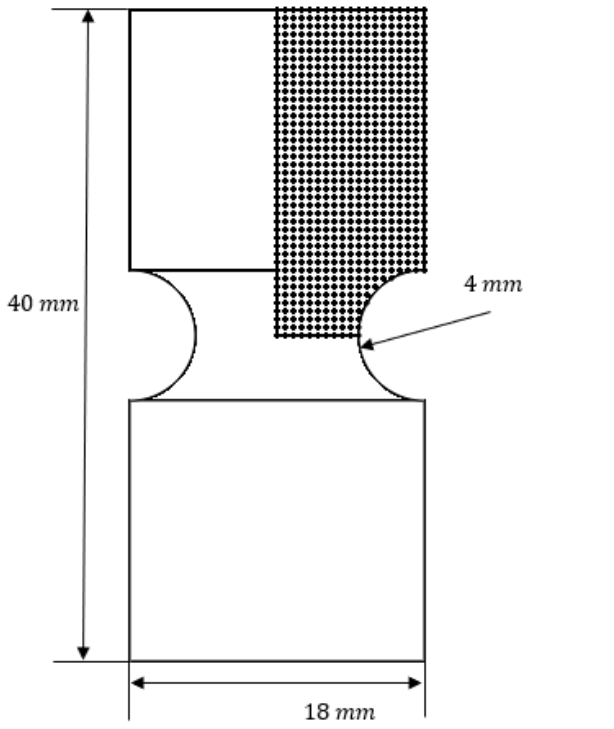
\includegraphics[width=0.4\textwidth]{./Figures/finiteVolumeImplementation/inhomogenousDeformation/axiNotchedCase.png}
\caption{Geometry of the notched round bar}
\end{center}
\end{figure}

\begin{figure}[htbp]
	\centering
		\subfigure[8000 cell mesh] {\label{airbus}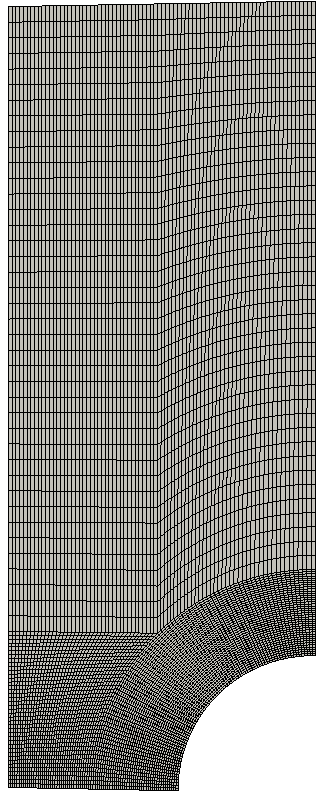
\includegraphics[width=0.3\textwidth]{./Figures/finiteVolumeImplementation/inhomogenousDeformation/axiNotchedMeshBW.png}}
		
		\subfigure[Marked cell in pink where results are analysed] {\label{boeing} 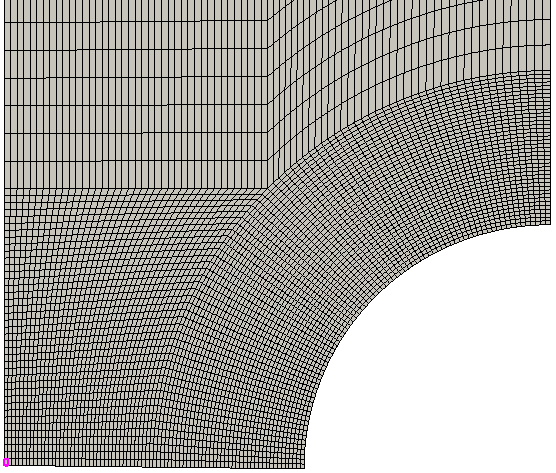
\includegraphics[width=0.3\textwidth]{./Figures/finiteVolumeImplementation/inhomogenousDeformation/markedCellAxi.png}}
		
		\caption{Notched round bar mesh}
	\label{fig:notched_bar_mesh}
\end{figure}

A vertical displacement of 1.0 \si{\milli\meter} is applied to the upper boundary over 100 quasi-static loading steps, corresponding to 0.01 \si{\milli\meter} increments.

Table \ref{tab:notched_bar_mat} gives the assumed elastoplastic material parameters.
\begin{table}[htb]
	\centering
		\begin{tabular}{llll} \hline
			Property & Symbol & Value  \\ \hline 
			Young's modulus & $E$ & $69$ GPa \\
			Poisson's ratio & $v$ & $0.3$   \\
			Hardening law & $\sigma_y$ & $589({0.0001+\bar{\varepsilon}}^p)^{0.216}$ MPa  \\
			\hline
		\end{tabular}
	\caption{Material properties for the notched round bar}
	\label{tab:notched_bar_mat}
\end{table}



%%%%%%%%%%%
\subsection{Flat Notched Bar}
%%%%%%%%%%%
The 3-D flat notched tensile specimen (Figure \ref{fig:flat_bar_geom}) is another common test case for assessing damage models, for example, as examined by \citet{borden_phase-field_2016} and \citet{eldahshan_phase_2021}.
The geometry consists of $152.4 \times 25.4$ \si{\milli\meter} plate with a 4.06 \si{\milli\meter} diamter side notches.
The solution domain consists of one-quarter of the specimen by exploiting three symmetry planes.
A structured hexahedral mesh is employed (Figure \ref{fig:flat_bar_mesh}).

\begin{figure}[htb] \label{fig:flat_bar_geom}
\begin{center}
	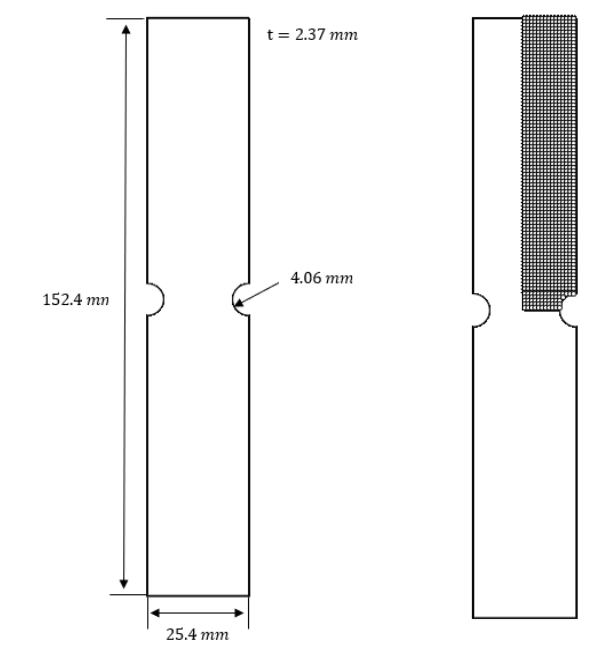
\includegraphics[width=0.6\textwidth]{./Figures/finiteVolumeImplementation/inhomogenousDeformation/flatNotchedTensile.png}
\caption{Geometry of the flat notched bar}
\end{center}
\end{figure}

\begin{figure}[htbp]
	\centering
		\subfigure[10000 cell mesh] {\label{airbus}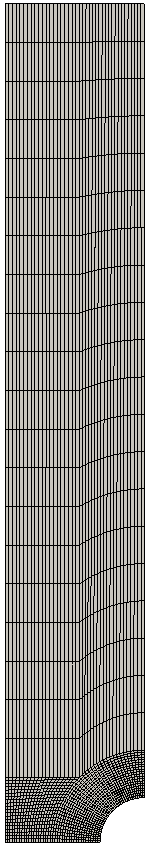
\includegraphics[width=0.1\textwidth]{./Figures/finiteVolumeImplementation/inhomogenousDeformation/bordenMesh.png}}
		
		\subfigure[Marked cell in pink where results are analysed] {\label{boeing} 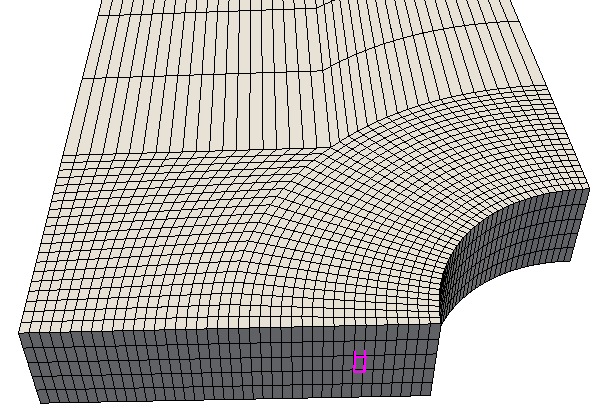
\includegraphics[width=0.3\textwidth]{./Figures/finiteVolumeImplementation/inhomogenousDeformation/bordenCell.png}}
		
		\caption{Flat notched bar mesh}
	\label{flat_bar_mesh}
\end{figure}

A vertical displacement of 1.143 \si{\milli\meter} is applied to the upper boundary over 100 quasi-static loading steps, corresponding to 0.01143 \si{\milli\meter} increments.

Table \ref{tab:flat_bar_mat} gives the assumed elastoplastic material parameters.
\begin{table}[htb]
	\centering
		\begin{tabular}{llll} \hline
			Property & Symbol & Value  \\ \hline 
			Young's modulus & $E$ & $68.8$ GPa \\
			Poisson's ratio & $v$ & $0.33$   \\
			Hardening law & $\sigma_y$ & $320+688\bar{\varepsilon}^p$ MPa  \\
			\hline
		\end{tabular}
	\caption{Material properties for the flat notched bar}
	\label{tab:flat_bar_mat}
\end{table}



%\subsection{Plasticity model} \label{PlasticityTestCases}

Before verifying the damage and fracture models, the implementation of the plasticity model described in chapter 3 is verified by comparing its results to (i) the elasto-plastic model implemented by  \citet{clancy_improving_2019}) in OpenFOAM that uses the logarithmic strain and the Mandel stress \cite{caminero_modeling_2011}, (ii) to the elasto-plastic model implemented in OpenFOAM by \citet{cardiff_lagrangian_2017}, which uses the Green strain tensor and the return mapping algorithm described by \citet{simo_computational_1998} and (iii) to results obtained from simulations conducted in Abaqus.

%These simulations are conducted using the material properties described in Tables 5.5 and 5.6.


%A displacement of $1.0\ mm$ is applied to the top boundary of the notched round bar specimen, with 100 time steps used in this simulation corresponding to increments of $0.01\ mm$. 
%
%A displacement of $1.143\ mm$ is applied to the top boundary of the flat notched bar specimen, with 100 time steps used in this simulation corresponding to increments of $0.01143\ mm$. 

\subsubsection{Reaction force vs displacement}

It can be seen in Figure 5.11 that the results align very well, verifying the implementation of this model. It is worth noting that the reaction force for both the \citet{clancy_improving_2019} implementation and the implementation of this work (which both use the logarithmic strain) is slightly less than that given by the \citet{cardiff_lagrangian_2017} implementation and the Abaqus simulation in the latter stages of the deformation. It is unclear exactly why this is, though it could be related to the fact that formulations which employ the logarithmic strain are not exactly mathematically equivalent to those which employ the Green strain tensor.

\begin{figure}[htbp]
	\centering
		\subfigure[Notched round bar] {\label{airbus}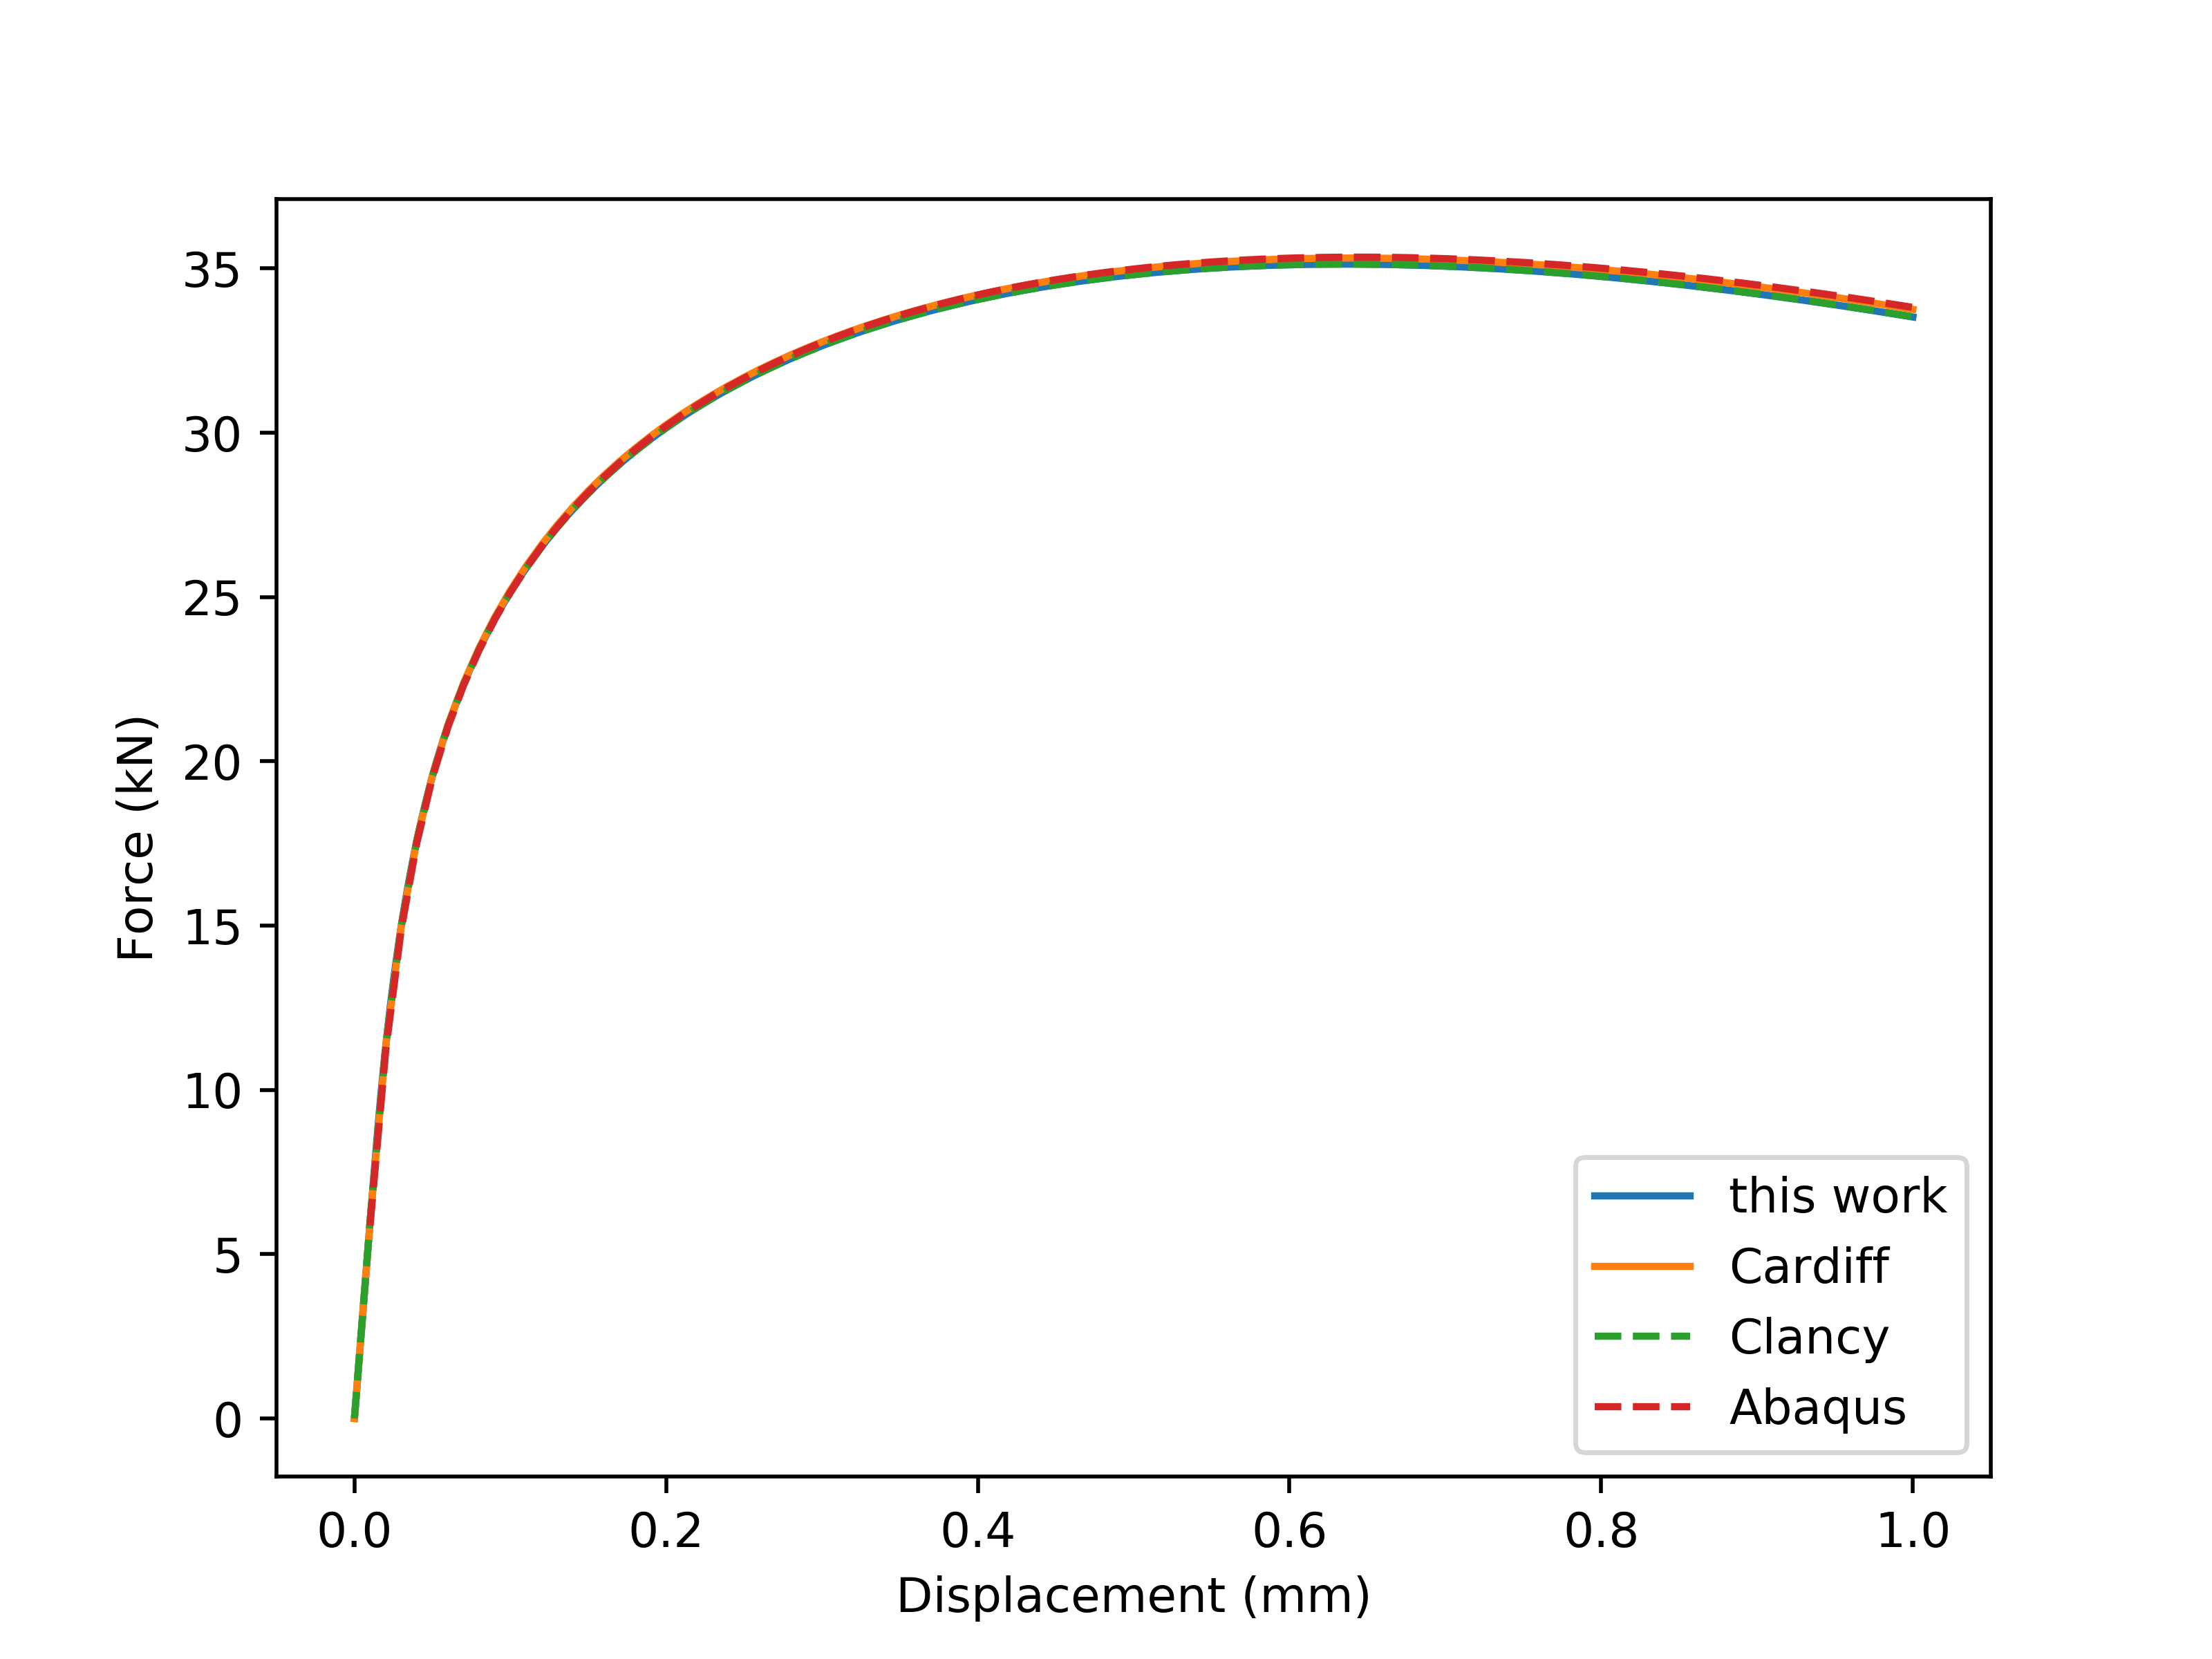
\includegraphics[width=0.8\textwidth]{./Figures/finiteVolumeImplementation/inhomogenousDeformation/forceDispAxi.png}}
		
		\subfigure[Flat notched bar] {\label{airbus}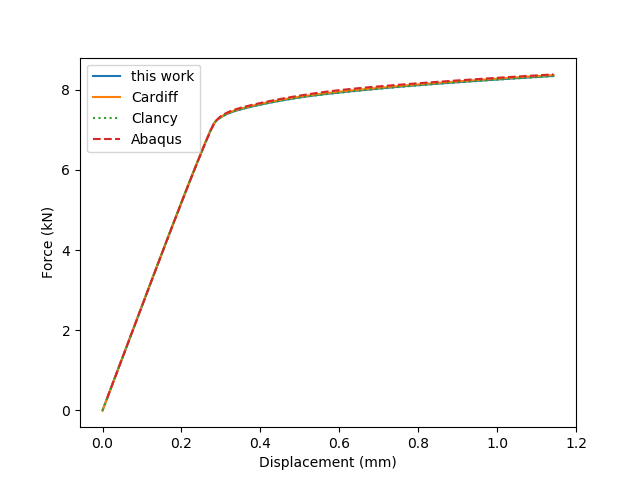
\includegraphics[width=0.8\textwidth]{./Figures/finiteVolumeImplementation/inhomogenousDeformation/forceDispBorden.png}}
		
		\caption{Force-displacement curves}
	\label{label_for_entire_figure}
\end{figure}
\FloatBarrier



\subsubsection{Results at cell centre of interest}

The results at the centroid of a chosen cell (marked in pink in Figures 5.9 and 5.10) are here compared for the implementation of this work, the \citet{cardiff_lagrangian_2017} implementation and the results from Abaqus. It is noticeable that in both test cases, the equivalent plastic strain is marginally greater in the OpenFOAM simulations than the Abaqus ones in the latter stages of the deformation. As can be seen in Appendix F, this discrepancy is unrelated to the time-step or mesh size discretisation error. Throughout this chapter, relatively fine meshes and small time steps are used to ensure that this form of error is negligible.

It is unclear exactly why this difference (or other small differences which will be encountered) later in the chapter exists, though it could be related to the fact that in Abaqus the Jaumann rate is used to update the stress tensor \cite{soyarslan_finite_2010}, unlike in OpenFOAM.

\subsubsection{Notched round bar}

For the NRB, the results for the cell at the centre of the specimen are compared (Figure 5.9). This cell is chosen because it is where fracture initiates for both the Lemaitre and GTN model simulations that will be encountered later in this chapter. 

\begin{figure}[htb]
\begin{center}
	\includegraphics[width=0.9\textwidth]{./Figures/plasticityCompare/axiCompare/disp_EpsPEq.png}
\caption{Equivalent plastic strain vs. displacement}
\label{fig:eqPlasticStrainNotchedRoundBar}
\end{center}
\end{figure}


\begin{figure}[htbp]
	\centering
		\subfigure[Equivalent stress vs. displacement] {\label{airbus}\includegraphics[width=0.6\textwidth]{./Figures/plasticityCompare/axiCompare/disp_sigmaEq.png}}
		
		\subfigure[Pressure vs. displacement] 
  {\label{airbus}\includegraphics[width=0.6\textwidth]{./Figures/plasticityCompare/axiCompare/disp_Pressure.png}}
		
		\subfigure[Sigma YY vs. displacement] 
  {\label{airbus}\includegraphics[width=0.6\textwidth]{./Figures/plasticityCompare/axiCompare/disp_sigmaYY.png}}
		
		\caption{Comparison of stress state}
	\label{label_for_entire_figure}
\end{figure}
\FloatBarrier

\subsubsection{Flat notched bar}

For the FNB, results are shown for the cell that is $6.912\ mm$ to the right of the centre of this specimen. This cell is chosen because it is where fracture initiates for the Lemaitre model (Figure 5.10).

\begin{figure}[htb]
\begin{center}
	\includegraphics[width=0.9\textwidth]{./Figures/plasticityCompare/bordenCompare/disp_EpsPEq.png}
\caption{Equivalent plastic strain vs. displacement}
\label{fig:notchedRoundBAr}
\end{center}
\end{figure}


\begin{figure}[htbp]
	\centering
		\subfigure[Equivalent stress vs. displacement] {\label{airbus}\includegraphics[width=0.6\textwidth]{./Figures/plasticityCompare/bordenCompare/disp_sigmaEq.png}}
		
		\subfigure[Pressure vs. displacement]
  {\label{airbus}\includegraphics[width=0.6\textwidth]{./Figures/plasticityCompare/bordenCompare/disp_Pressure.png}}
		
		\subfigure[Sigma YY vs. displacement]
  {\label{airbus}\includegraphics[width=0.6\textwidth]{./Figures/plasticityCompare/bordenCompare/disp_sigmaYY.png}}
		
		\caption{Comparison of stress state}
	\label{label_for_entire_figure}
\end{figure}
\FloatBarrier

\subsubsection{Lemaitre model}

\begin{table}[htb]
	\centering
		\begin{tabular}{cccc} \hline
			Property & Symbol & Value  \\ \hline 
			Young's modulus & $E$ & $69.9$ GPa \\
			Poisson's ratio & $v$ & $0.3$   \\
			Lemaitre damage denominator & $S_0$ & $1.1$ MPa  \\
			Lemaitre damage exponent & $b$ & 1.0  \\
			Characteristic Length & $l_c$ & $0.6325$ mm  \\
			Hardening law & $\sigma_y$ & $589({0.0001+\bar{\varepsilon}}^p)^{0.216}$ MPa \\
			\hline
		\end{tabular}
	\caption{Material properties for the NRB}
	\label{tab:material_properties}
\end{table}

A displacement of $0.8\ mm$ is applied to the top boundary of the NRB specimen, with 800 time steps used in these simulations corresponding to displacement increments of $0.001\ mm$. The material properties in Table 5.7 are taken from \citet{cesar_de_sa_damage_2006}.

The distribution of the non-local damage at a displacement of $0.6\ mm$ in the OpenFOAM simulation is compared with the results provided in \citet{cesar_de_sa_damage_2006} in Figure 5.16. In both of these cases the non-local damage reaches a maximum of $\approx0.5$, it is clear that in both of these simulations the distribution of the damage over the specimen follows a similar pattern.

\begin{figure}[t!]
	\centering
		\subfigure[Results from \cite{cesar_de_sa_damage_2006}] {\label{airbus}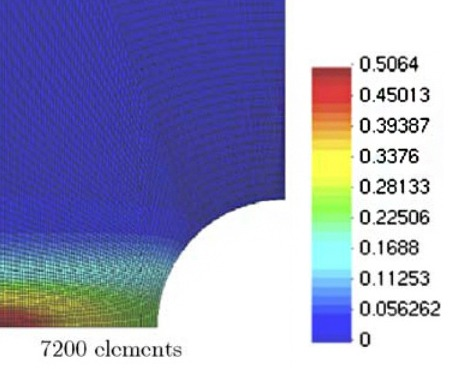
\includegraphics[width=0.4\textwidth]{./Figures/LemaitreCompare/updated_deSaNonLocal.jpeg}}
		\qquad
		\subfigure[OpenFOAM simulation] {\label{boeing} 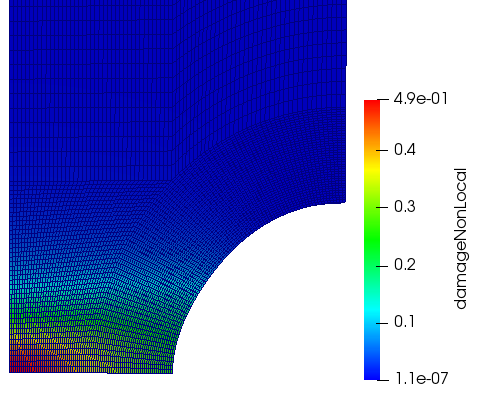
\includegraphics[width=0.4\textwidth]{./Figures/LemaitreCompare/nlDamageLemaitre.png}}
		
		\caption{Comparison of non-local damage distribution}
	\label{label_for_entire_figure}
\end{figure}
\FloatBarrier

\subsubsection{Lemaitre model: Abaqus vs. OpenFOAM}

In this sub-section results from the OpenFOAM and Abaqus implementations of the non-local gradient Lemaitre model are compared. It can be seen in Figure 5.17, that the OpenFOAM simulation of the non-local gradient Lemaitre model localises at a slightly quicker rate than the Abaqus implementation. This has been encountered earlier in the comparison of the equivalent plastic strain in section 5.3.2. The marginally faster increase of the equivalent plastic strain and damage results in a slightly quicker loss of load-carrying capacity for the specimen, as can be observed in Figure 5.18.

\begin{figure}[htb]
\begin{center}
	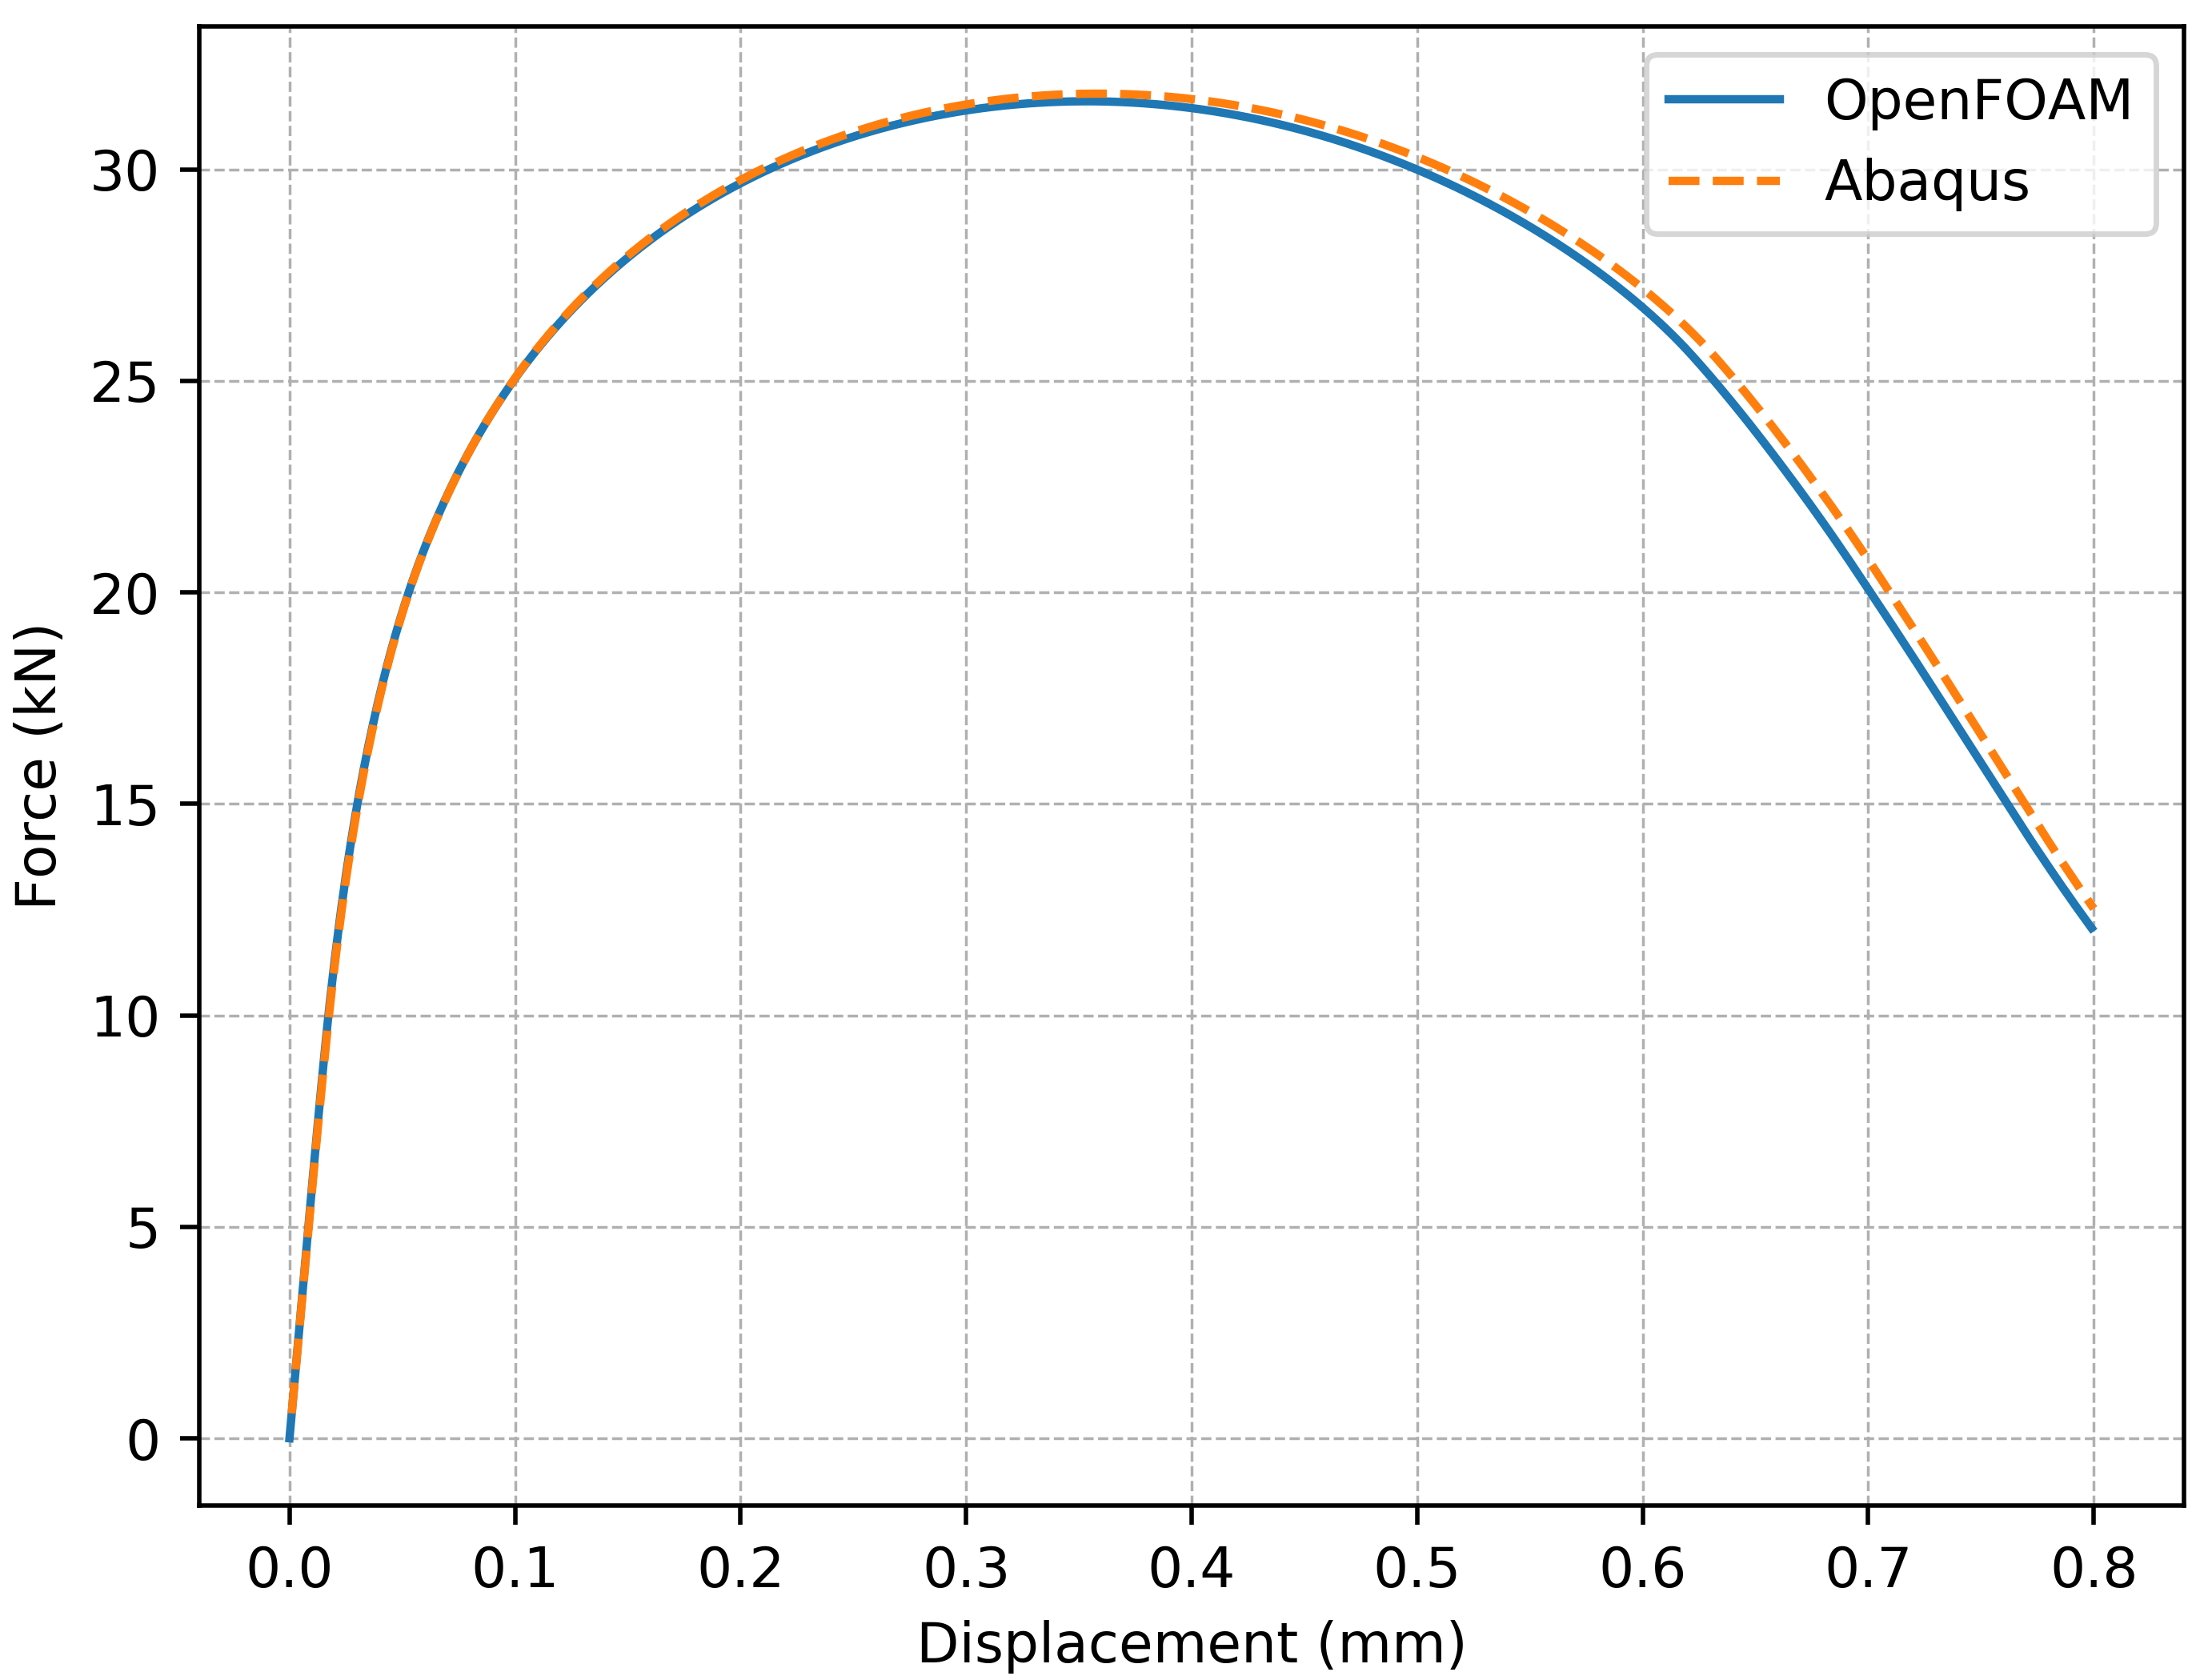
\includegraphics[width=0.9\textwidth]{./Figures/LemaitreCompare/axiCompare/1.1LemaitreCompare.png}
\caption{Force vs. displacement}
\label{fig:notchedRoundBAr}
\end{center}
\end{figure}

\begin{figure}[t!]
	\centering
		\subfigure[Non-local damage vs.displacement (mm)] {\label{airbus}\includegraphics[width=0.6\textwidth]{./Figures/LemaitreCompare/axiCompare/disp_damageNonLocal.png}}
	
		\subfigure[Equivalent plastic strain vs. displacement] {\label{boeing} \includegraphics[width=0.6\textwidth]{./Figures/LemaitreCompare/axiCompare/disp_EpsPEq.png}}
		
		\caption{Abaqus and OpenFOAM implementations comparison}
	\label{label_for_entire_figure}
\end{figure}
\FloatBarrier

\textbf{Flat notched bar}

Simulations are also performed on the flat notched bar case. Displacement increments of $0.001143\ mm$ are applied by default in this case until the rapid loss of load-carrying capacity is observed. For the Abaqus case, the option was given for the simulation to use displacement increments as small as $0.00001143\ mm$, via the adaptive time stepping scheme available in this software.

\begin{table}[htb]
	\centering
		\begin{tabular}{cccc} \hline
			Property & Symbol & Value  \\ \hline 
			Young's modulus & $E$ & $68.9$ GPa \\
			Poisson's ratio & $v$ & $0.33$   \\
			Lemaitre damage denominator & $S_0$ & $0.5$ MPa  \\
			Lemaitre damage exponent & $b$ & 1.0  \\
			Characteristic Length & $l_c$ & $0.6325$ mm  \\
			Hardening law & $\sigma_y$ & $320+688\times\bar{\varepsilon}^p$ MPa \\
			\hline
		\end{tabular}
	\caption{Material properties for the FNB}
	\label{tab:material_properties}
\end{table}

It is clear from Figure 5.19 that the results align well. Again it can be observed that there are slightly quicker increases in the damage and equivalent plastic strain for the OpenFOAM simulation (Figure 5.20). It is worth noting that Abaqus struggles to converge in the rapid crack propagation stage of this simulation, with it requiring very small displacement increments until it eventually crashes after a total displacement of $~0.463\ mm$. By contrast, no such issues were encountered with the OpenFOAM simulation.

Further tests were conducted for different values of $S_0$ (Figure 5.21). As the value of $S_0$ is increased, the rapid crack propagation occurs later in the deformation process. It is noticeable that the discrepancies between OpenFOAM and Abaqus simulations are larger the later in the deformation process that fracture occurs.

\begin{figure}[htb]
\begin{center}
	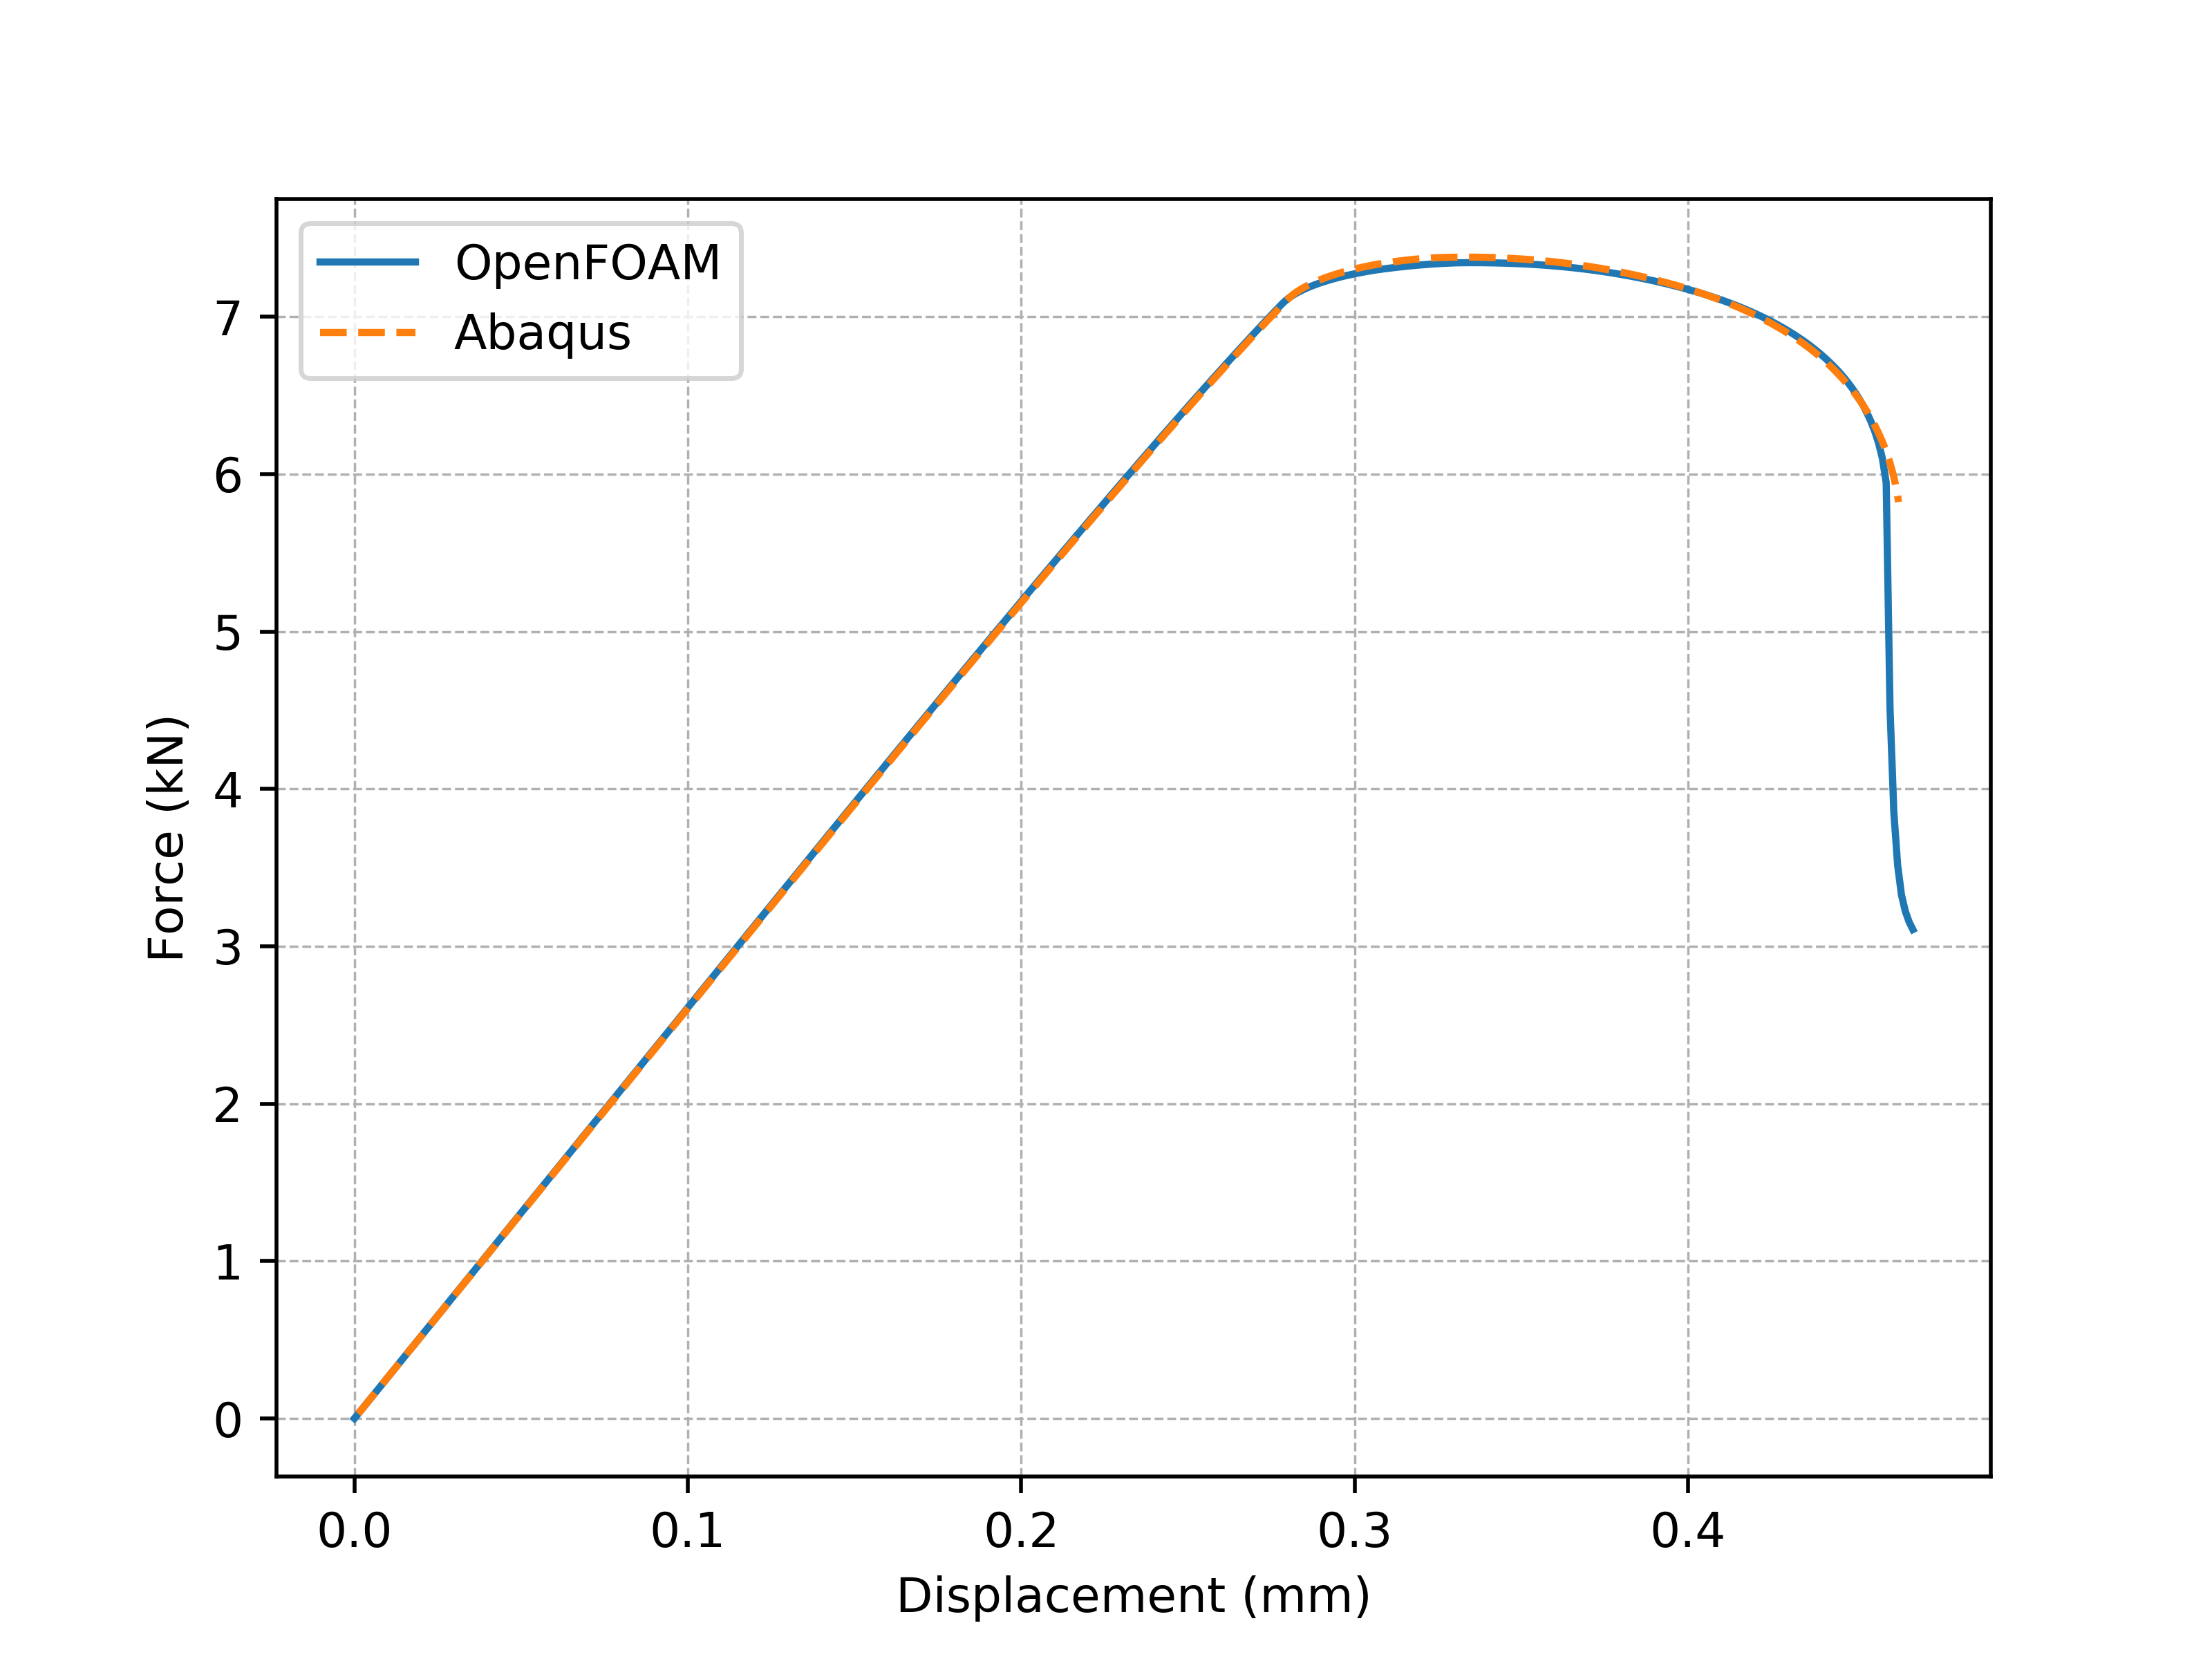
\includegraphics[width=0.9\textwidth]{./Figures/LemaitreCompare/borden/bordenDispForce.png}
\caption{Force vs. displacement}
\label{fig:notchedRoundBAr}
\end{center}
\end{figure}

\begin{figure}[t!]
	\centering
		\subfigure[Displacement vs. non-local Damage] {\label{airbus}\includegraphics[width=0.6\textwidth]{./Figures/LemaitreCompare/borden/disp_damageNonLocal.png}}
	
		\subfigure[Displacement vs. equivalent plastic strain] {\label{boeing} \includegraphics[width=0.6\textwidth]{./Figures/LemaitreCompare/borden/disp_EpsPEq.png}}
		
		\caption{Abaqus and OpenFOAM implementations comparison}
	\label{label_for_entire_figure}
\end{figure}
\FloatBarrier

\begin{figure}[htb]
\begin{center}
	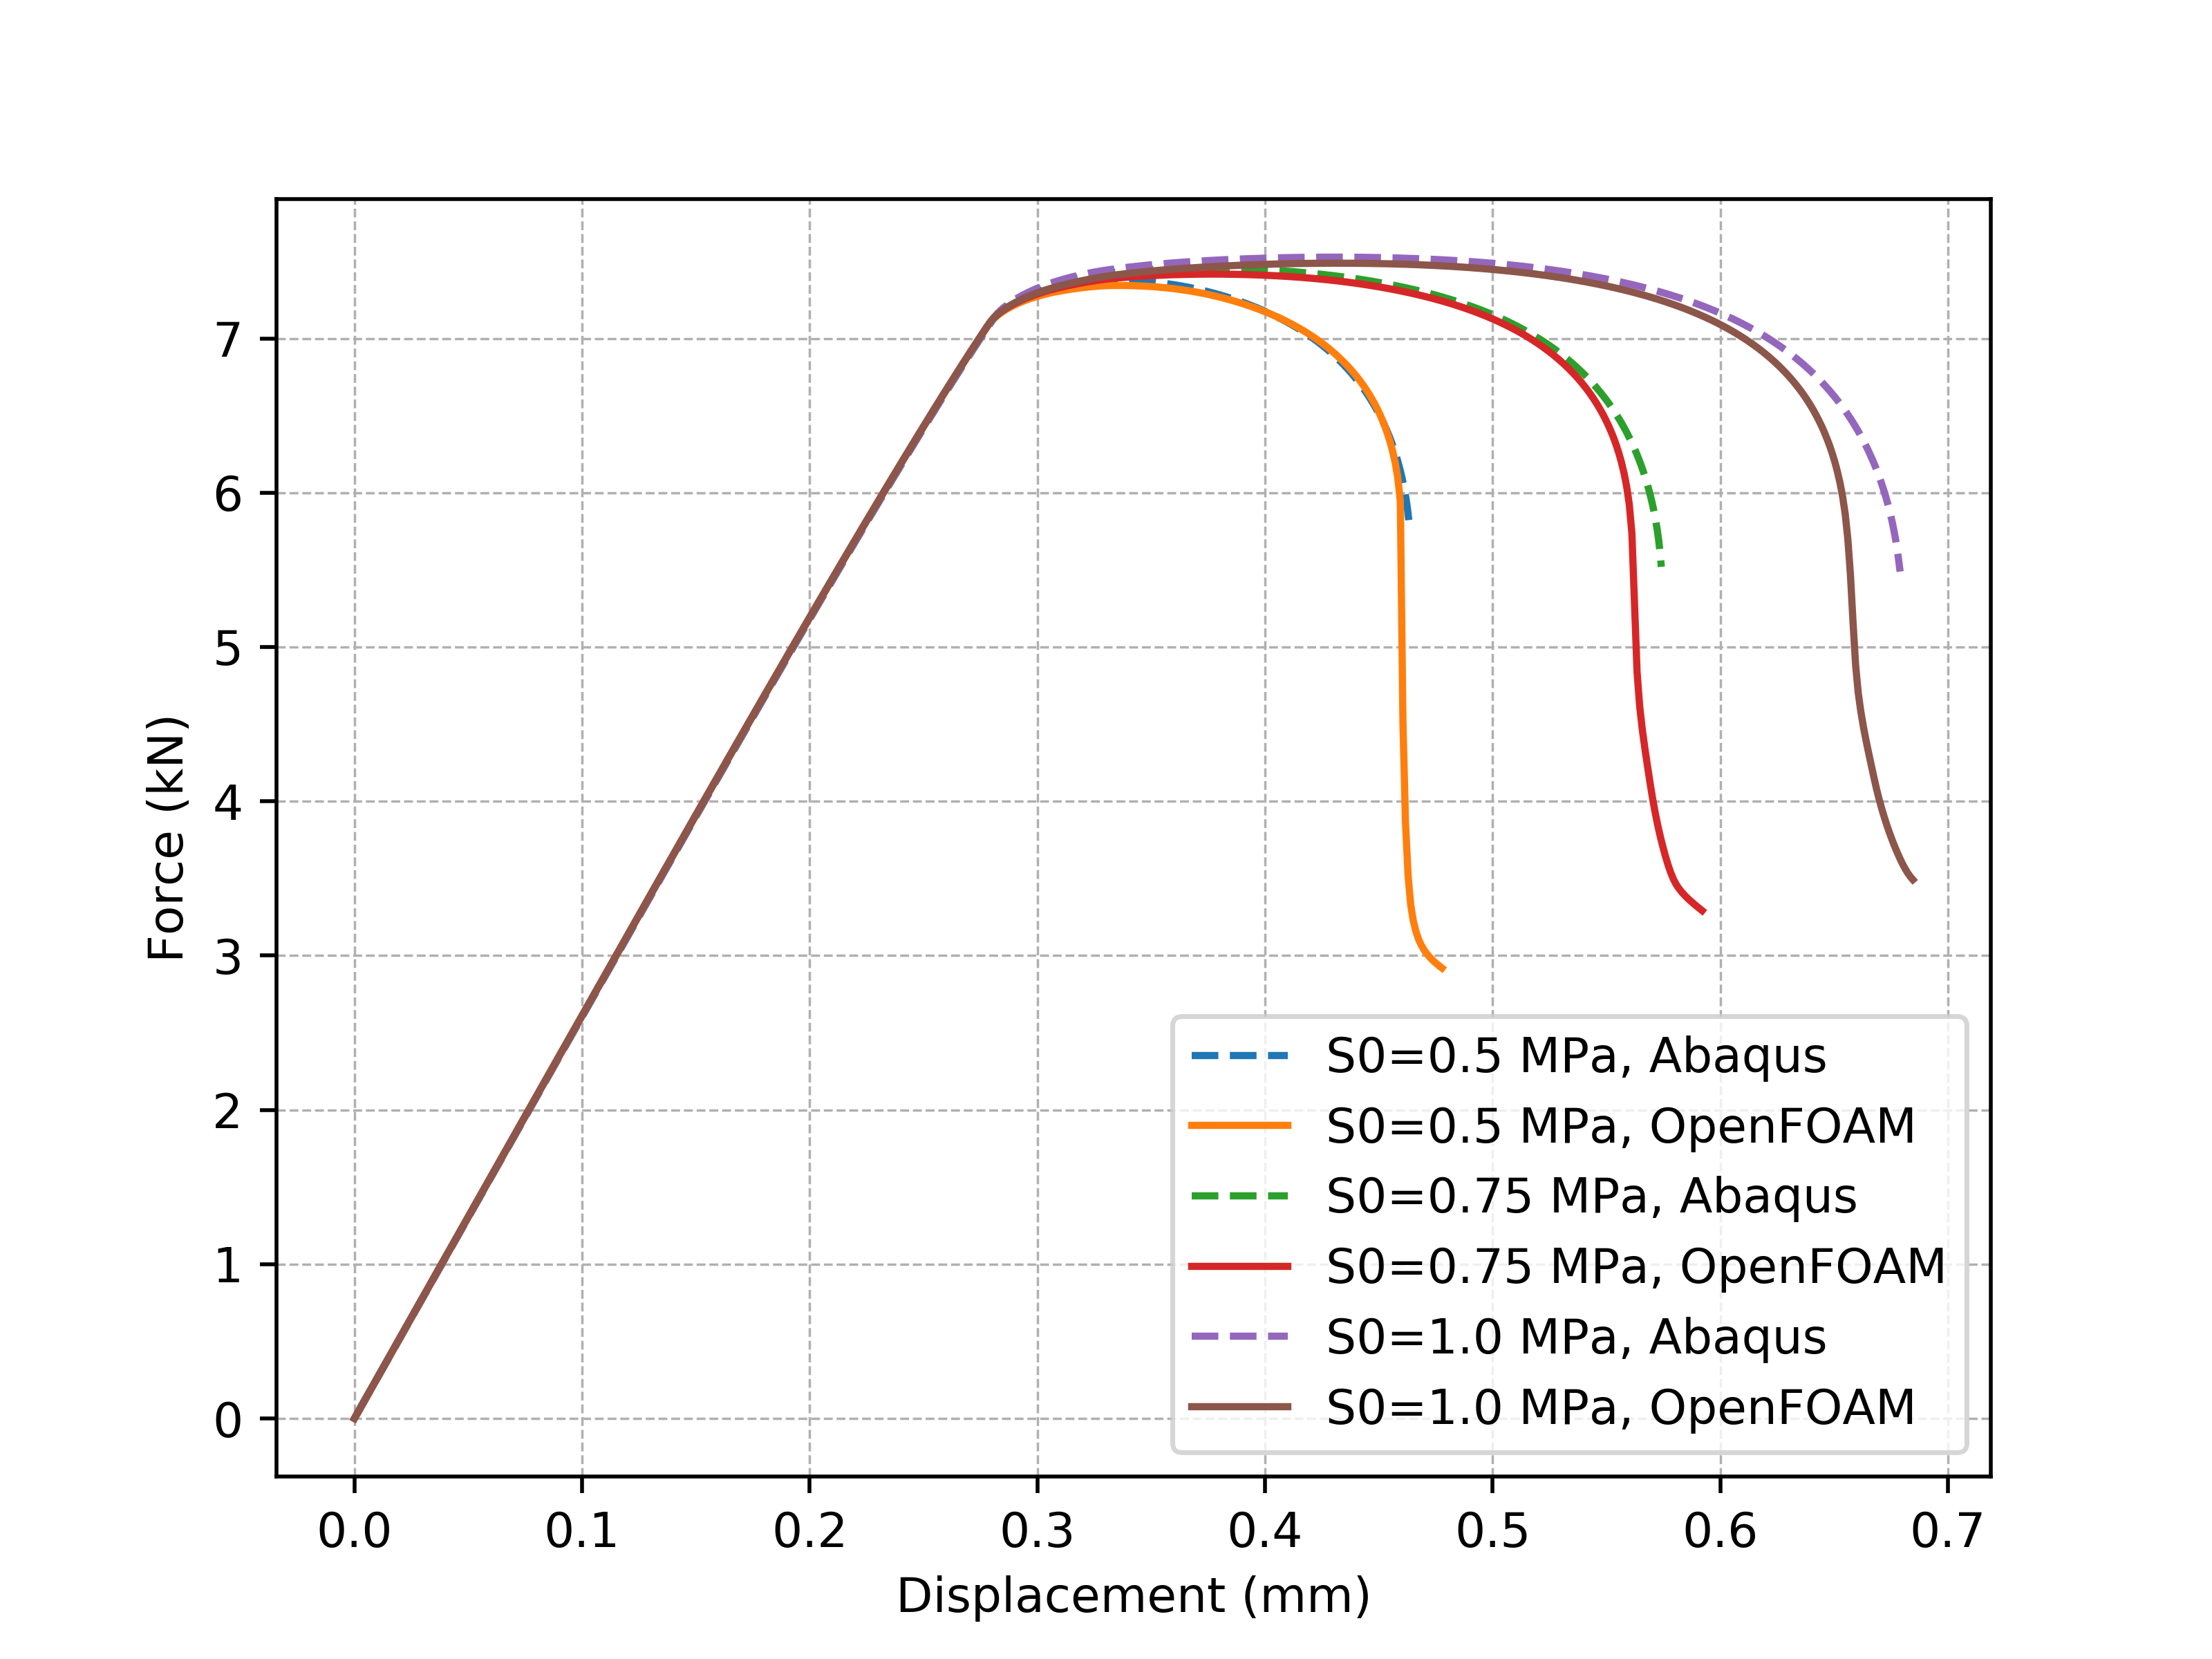
\includegraphics[width=0.9\textwidth]{./Figures/LemaitreCompare/borden/lemaitreBordenCompare.png}
\caption{Force vs. displacement for different values of $S_0$}
\label{fig:notchedRoundBAr}
\end{center}
\end{figure}
\FloatBarrier

\subsubsection{GTN model}

\begin{table}[htb]
	\centering
		\begin{tabular}{cccc} \hline
			Property & Symbol & Value  \\ \hline 
			Young's modulus & $E$ & $69$ GPa \\
			Poisson's ratio & $v$ & $0.3$   \\
			q1 & $q1$ & $1.5$  \\
		    q2 & $q2$ & $1$  \\
		    q3 & $q3$ & $2.25$  \\
		    Initial porosity & $f_0$ & $0.002$  \\
		    Mean & $\varepsilon_n$ & $0.15$  \\
		    Standard deviation & $S_n$ & $0.08$  \\
		    Volume fraction & $f_N$ & $0.2$  \\
			Hardening law & $\sigma_y$ & $589({0.0001+\bar{\varepsilon}}^p)^{0.216}$ MPa  \\
			\hline
		\end{tabular}
	\caption{Material properties for the NRB}
	\label{tab:material_properties}
\end{table}

In this section, simulations are conducted on the implemented GTN model in OpenFOAM as well as on Abaqus using the inbuilt GTN model. A displacement of $0.5\ mm$ is applied. Increments of displacement of $0.001\ mm$ are applied by default. The Abaqus simulation is given the option to use increments as small as $0.00001\ mm$ to aid with convergence. 

In Figure 5.22, it can be seen that the results align reasonably well. As with the simulations conducted with the Lemaitre model, quicker localisation can be observed. A feature of this test case is the sharp crack propagation (Figure 5.23). The Abaqus simulation has convergence issues and eventually crashes at a displacement of $~0.371\ mm$. No such convergence issues were encountered with OpenFOAM. The superior convergence abilities of the OpenFOAM simulations are likely due to the fact that is uses the segregated-solution procedure (Section 2.7.3). By contrast, the Abaqus simulations require the calculation of the tangent stiffness matrix, which is derived during the finite element solution process. For elasto-plastic damage models, plastic deformation influences the onset and progression of damage, and vice versa. This interaction can result in a significant coupling in the tangent stiffness matrix, manifesting as non-trivial off-diagonal terms \cite{bathe_finite_1996}. These terms can introduce convergence difficulties.

\begin{figure}[htb]
\begin{center}
	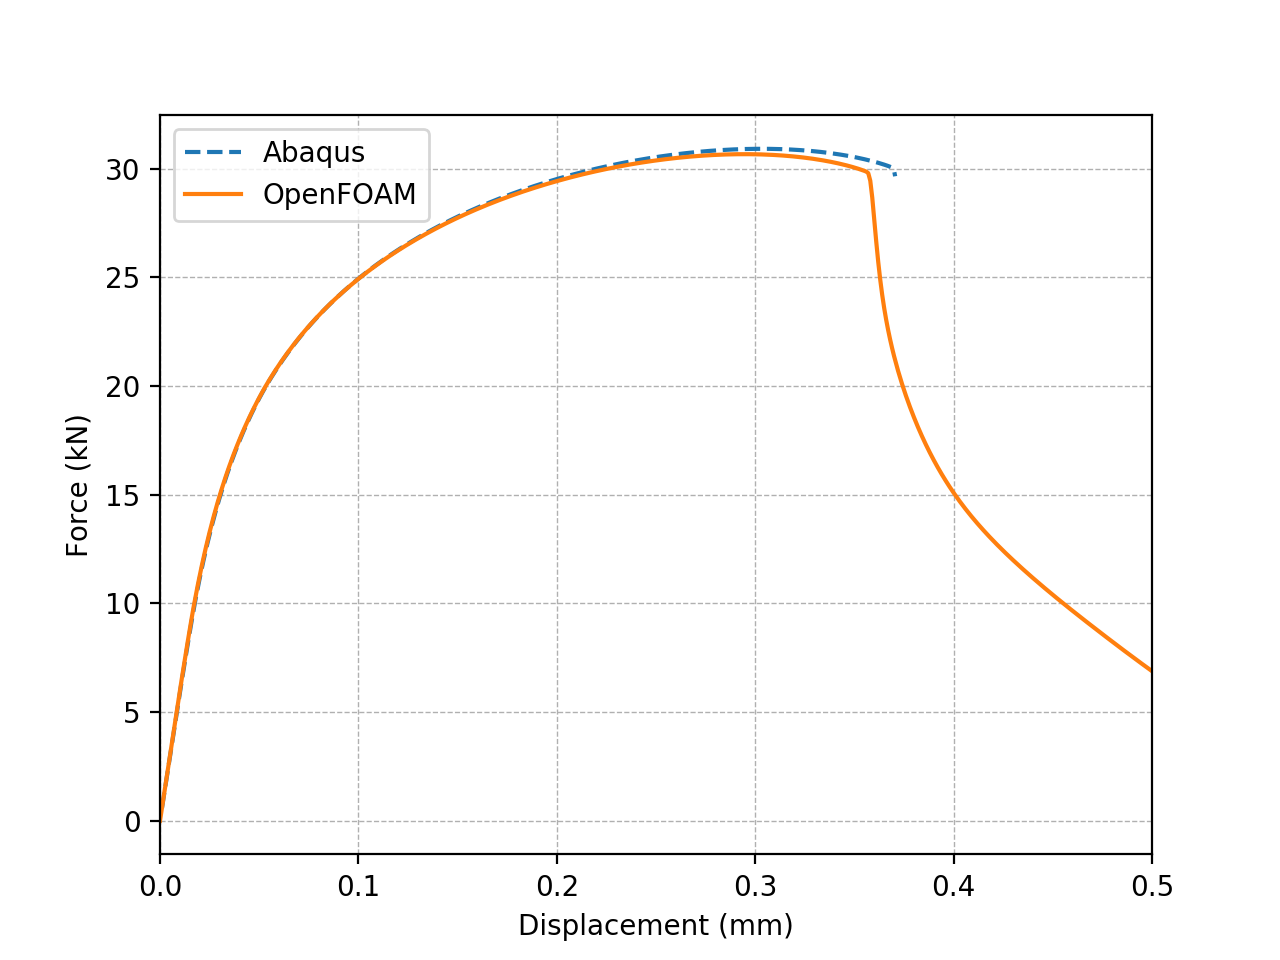
\includegraphics[width=0.7\textwidth]{./Figures/GTNCompare/forceDispGTN.jpg}
\caption{Force vs. displacement}
\label{fig:notchedRoundBAr}
\end{center}
\end{figure}

\begin{figure}[t!]
	\centering
		\subfigure[Porosity vs. displacement] {\label{airbus}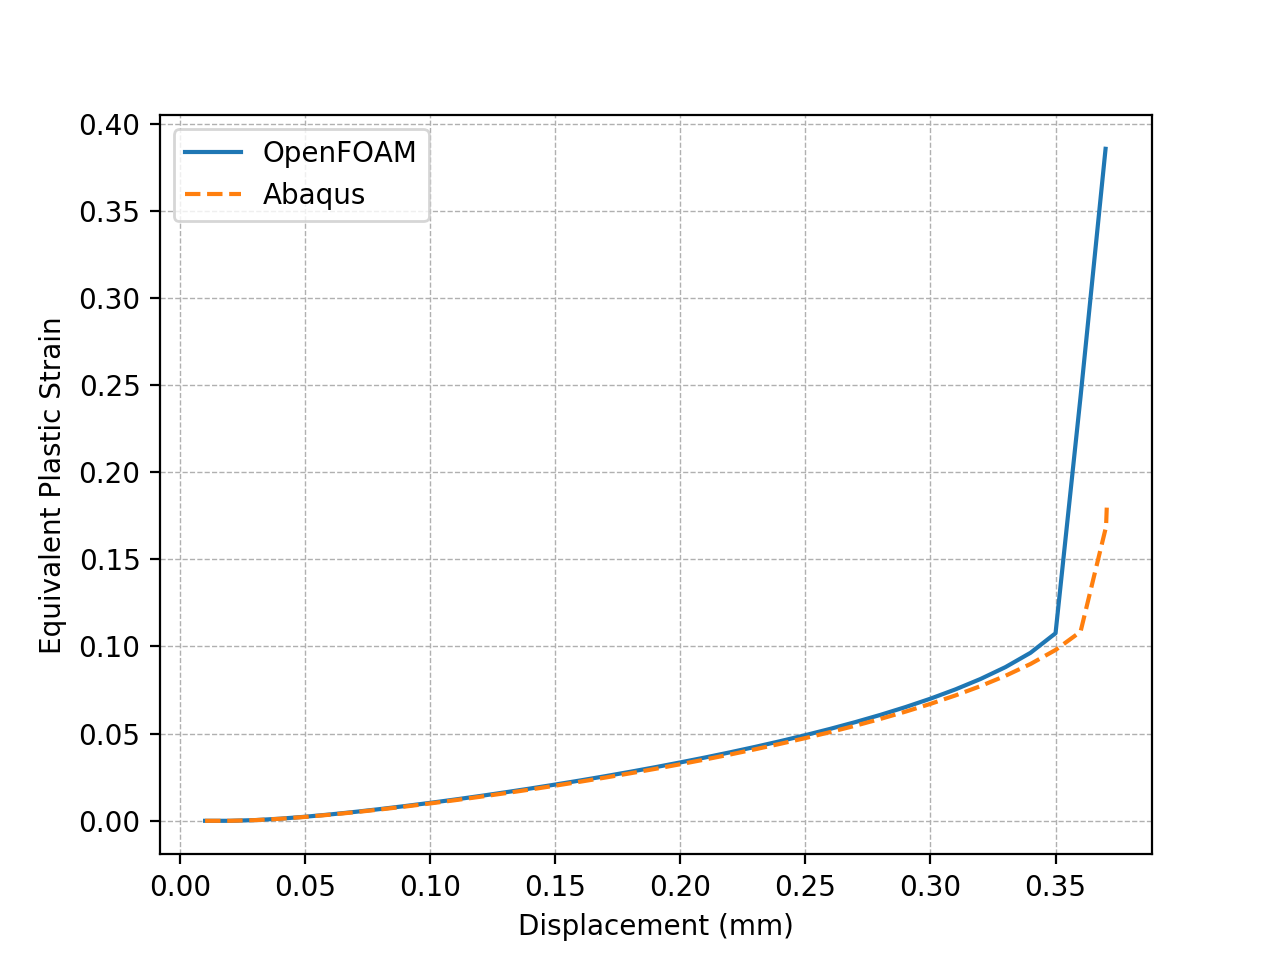
\includegraphics[width=0.6\textwidth]{./Figures/GTNCompare/epsilonPEq_GTN.jpg}}
	
		\subfigure[Equivalent plastic strain vs. displacement] {\label{boeing} 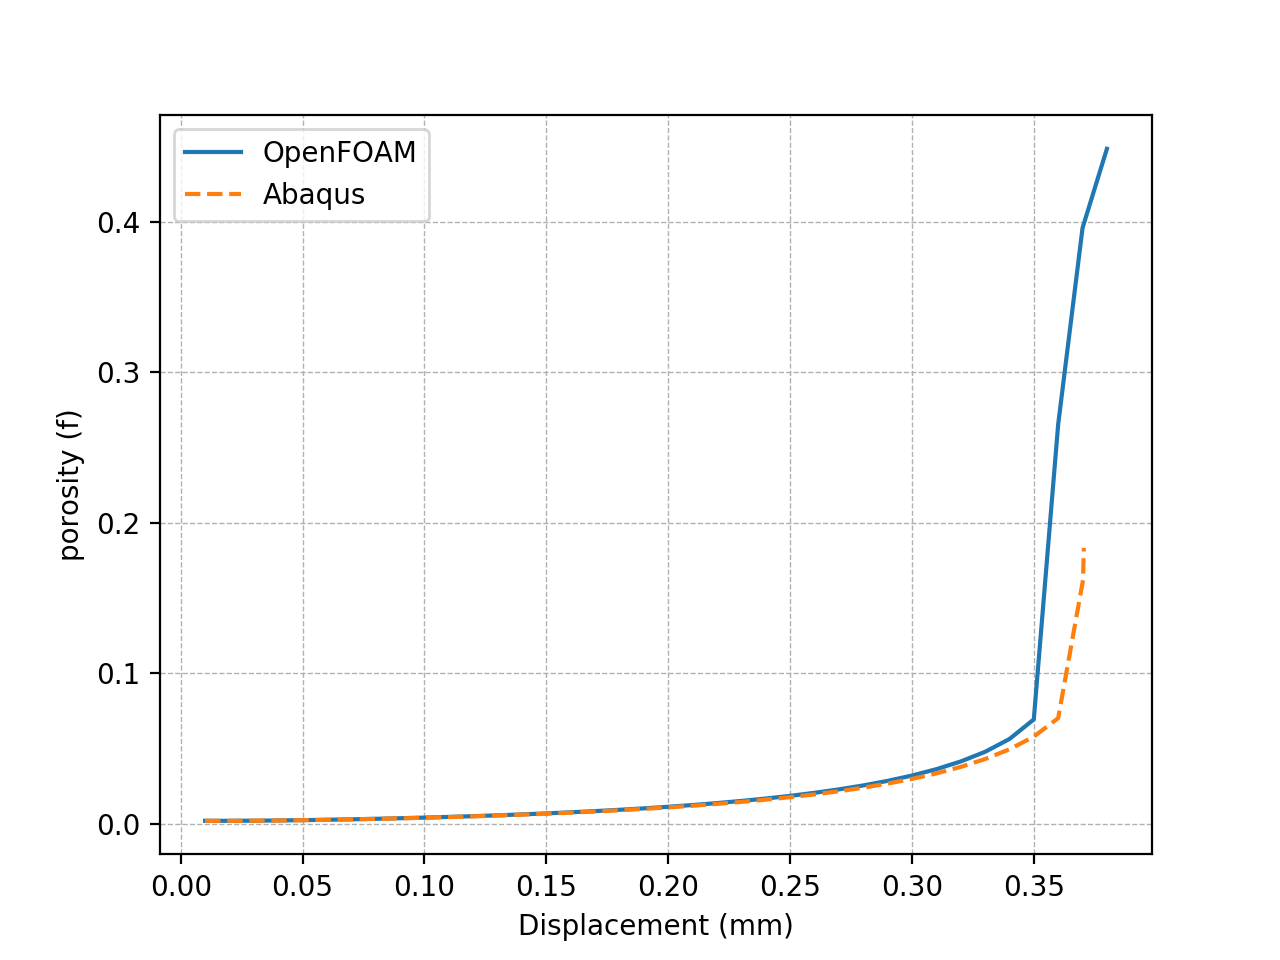
\includegraphics[width=0.6\textwidth]{./Figures/GTNCompare/displacement_porosity.jpg}}
		
		\caption{Abaqus and OpenFOAM implementations comparison}
	\label{label_for_entire_figure}
\end{figure}
\FloatBarrier

\subsubsection{Phase field fracture}

\begin{table}[htb]
	\centering
		\begin{tabular}{cccc} \hline
			Property & Symbol & Value  \\ \hline 
			Young's modulus & $E$ & $68.8$ GPa \\
			Poisson's ratio & $v$ & $0.33$   \\
			Critical Fracture Energy & $G_c$ & $60\times10^3$ $J/m^2$ \\
			Plastic Threshold & $W_o$ & $1\times10^7$ MPa \\
			Characteristic Length & $l_c$ & $0.3226mm$    \\
			Hardening law & $\sigma_y$ & $320+688\times{\bar{\varepsilon}}^p$ MPa  \\
			\hline
		\end{tabular}
	\caption{Material properties for phase field fracture FNB}
	\label{tab:material_properties}
\end{table}

In this section, OpenFOAM simulations are conducted for the flat notched bar case in \citet{borden_phase-field_2016}. The material properties are given in Table 5.10. Displacement increments of $0.001143\ mm$ are used until fracture has occurred. The results obtained are compared with those from \citet{borden_phase-field_2016} and \citet{eldahshan_phase_2021}. 

It can be seen that the results line up well, verifying the implementation of the model. It is worth noting that the normalised stress reported by \citet{borden_phase-field_2016} prior to the rapid crack propagation is slightly lower than that obtained both here and by \citet{eldahshan_phase_2021}.

\begin{figure}[htb]
\begin{center}
	\includegraphics[width=0.8\textwidth]{./Figures/phaseCompare.png}
\caption{Normalised stress vs normalised strain}
\label{fig:notchedRoundBAr}
\end{center}
\end{figure}




\subsection{Wire drawing simulations}

\begin{figure}[htb]
\begin{center}
	\includegraphics[width=0.7\textwidth]{./Figures/SimulationAndAnalysis/modelCompare/drawingSchematic.png}
\caption{Schematic of the wire drawing process}
\label{fig:notchedRoundBAr}
\end{center}
\end{figure}

\begin{figure}[htb]
\begin{center}
	\includegraphics[width=0.7\textwidth]{./Figures/SimulationAndAnalysis/wireMesh_InletOutlet.jpg}
\caption{Process for cell layer addition and removal}
\label{fig:wireInletOutlet}
\end{center}
\end{figure}



A schematic of the wire drawing process is given in Figure 7.1. A wire of initial diameter $D_i$ is pulled through a die of outlet diameter $D_o$. The reduction ratio $r\ (\%)$ is given by
\begin{equation}
    r=\left(\frac{d_i^2-d_o^2}{d_i^2}\right)\times100
\end{equation}
The die semi-angle $\alpha\ (^{\circ})$ is the angle made by the die with the horizontal (Figure 7.3).
For these wire-drawing simulations, an Eulerian-inspired Lagrangian method is employed \cite{cardiff_eulerian-inspired_2017}. In this approach, as the wire is being pulled through the die, cells are added to the wire at the inlet (or upstream) boundary and cells are deleted from the mesh at the outlet (or downstream) boundary (Figure 7.2). The simulation is
carried out until consistent values are reached along the wire for its properties after exiting the outlet patch. The wire is continuously being pulled in the axial direction by a fixed increment of displacement at each time step. More details on this procedure can be seen in \citet{cardiff_eulerian-inspired_2017}. The contact boundary is handled using the method developed in \citet{cardiff_development_2012,cardiff_lagrangian_2017}.

For these wire drawing cases, an initial contact is applied so that at the first step, the simulation is as shown in Figure 7.3. This can lead to localisations of plastic strain in the region of the wire in contact with the die. As the simulation moves forward a quasi steady-state solution is obtained. 


\begin{figure}[t!]
	\centering
		\subfigure[Initial contact at first time step] {\label{airbus}\includegraphics[width=0.8\textwidth]{./Figures/SimulationAndAnalysis/initialContact.png}}		
	  \qquad
		\subfigure[Equivalent plastic strain after $30\ mm$ displacement] {\label{boeing} \includegraphics[width=0.8\textwidth]{./Figures/SimulationAndAnalysis/settledEpsilonPEq.png}}
        \qquad
  	\subfigure[Damage after $30\ mm$ displacement] {\label{boeing} \includegraphics[width=0.8\textwidth]{./Figures/SimulationAndAnalysis/settledDamage.png}}
		
		\caption{Wire drawing simulation}
	\label{label_for_entire_figure}
\end{figure}
\FloatBarrier

\subsubsection{Incorporating damage}

This setup can lead to issues when incorporating damage, particularly in cases with large reduction ratios and high die angles which will be encountered in section 7.3. The high amount of deformation in this region of the wire in contact with the die in the initial time steps may lead to a large amount of damage accruing and an unstable numerical solution. It was found that this issue can be ameliorated by setting the damage to only begin evolving in the wire after the wire has already gone through a user-defined displacement. 

\begin{figure}[htb]
\begin{center}
	\includegraphics[width=0.7\textwidth]{./Figures/SimulationAndAnalysis/damageIssue.png}
\caption{Issue with incorporating damage at initial stages of case}
\label{fig:notchedRoundBAr}
\end{center}
\end{figure}

\FloatBarrier

\subsection{Comparison of damage and fracture models}

In the wire drawing process, fracture typically originates in the centre of the specimen \cite{gonzalez_assessment_2018,norasethasopon_prediction_2008,hoffmanner_selection_1971,choi_study_2010}. In this section, simulations are conducted for a typical wire drawing pass, with a reduction ration $r$ of 10\% and a drawing semi-angle $\alpha$ of $6^{\circ}$ \cite{roh_process_2021}. The wire drawing simulations were performed in serial on the UCD Sonic High Performance Computing (HPC) cluster.

The loading conditions and material parameters used are given in Tables 7.1-7. The material parameters for the die are taken from \citet{clancy_improving_2019}. The elasto-plastic parameters of the wire used are similar to the ones that will be calibrated in section 7.3 for high-carbon steel. For the Lemaitre model with crack-closure effects, the crack-closure parameter is taken to be 0.2, as is typically the case for steels \cite{desmorat_modeling_2008,lemaitre_course_1996,bouchard_enhanced_2011}. Aside from this, the parameters taken for the GTN, phase field and Lemaitre damage model are somewhat arbitrary and are mainly chosen for illustrative purposes. The values of these parameters will not affect the area of the wire where damage or fracture is predicted to occur but rather the level of damage or porosity that accumulates.

\begin{table}[htb]
	\centering
		\begin{tabular}{cccc} \hline
		    %Loading Conditions \\ \hline 
		    Applied total displacement & $u$ & $30\ mm$ \\
		    Time step & $\Delta t$ & $0.001\ s$ \\
			Displacement increment  & $\Delta u$ & $0.2\ mm$   \\
			Friction coefficient & $\mu$ & $0.1$ \\
			\hline
		\end{tabular}
	\caption{Loading conditions for wire drawing case}
	\label{tab:material_properties}
\end{table}

\begin{table}[htb]
	\centering
		\begin{tabular}{cccc} \hline
		    %Loading Conditions \\ \hline 
		    Die inlet diameter & $16\ mm$ \\
		    Die outer diameter & $20\ mm$ \\
      	Die outlet Diameter & $12.33\ mm$ \\
            Die semi-angle &  $6^{\circ}$ \\
		    Wire length & $30\ mm$ \\
		    Initial wire diameter & $13\ mm$ \\
      	Die cell size & $0.4\ mm$ \\
            Wire cell size & $0.4\ mm$ \\
			\hline
		\end{tabular}
	\caption{Die and wire geometry}
	\label{tab:material_properties}
\end{table}


\begin{table}[htb]
	\centering
		\begin{tabular}{cccc} \hline
			Term  & Value  \\ \hline 
            Young's modulus & 200 $GPa$ \\
			Poisson's ratio & 0.3  \\
   		Hardening law & $689+(1340-689+250\times\bar{\varepsilon}^p)(1-e^{-32.82\times\bar{\varepsilon}^p})\ MPa$ &  \\
			\hline
		\end{tabular}
	\caption{Wire elasto-plastic material parameters}
	\label{tab:material_properties}
\end{table}

\begin{table}[htb]
	\centering
		\begin{tabular}{cccc} \hline
			Term  & Value  \\ \hline 
            Young's modulus & 600 $GPa$ \\
			Poisson's ration & 0.22  \\
			\hline
		\end{tabular}
	\caption{Die material parameters}
	\label{tab:material_properties}
\end{table}


\FloatBarrier

\subsubsection{Lemaitre model}

\begin{table}[htb]
	\centering
		\begin{tabular}{cccc} \hline
			Property & Symbol & Value  \\ \hline 
			Lemaitre damage denominator & $S_0$ & $13.5$ MPa  \\
			Lemaitre damage exponent & $b$ & 1.0  \\
            Crack closure parameter & $h$ & 0.2 \\
			\hline
		\end{tabular}
	\caption{Lemaitre model parameters}
	\label{tab:material_properties}
\end{table}

Simulations are here conducted for the Lemaitre damage model both with and without crack-closure effects. The resultant damage distributions are provided in Figures 7.5 and 7.6. 

In Figure 7.5 (a), it can be observed that without crack-closure effects, the Lemaitre model gives a somewhat unrealistic damage distribution with damage being at a maximum away from the centre of the wire. This is due to the fact that it does not distinguish between positive and negative triaxialities.  As a consequence of the triaxiality cut-off  $\left(-\frac{1}{3}\right)$ for damage evolution, there is limited damage evolution towards the upper area of the wire.

By contrast, for the Lemaitre model with crack-closure effects, the damage is at a maximum at the centre of the bar. This is due to the fact that this is where the triaxiality, and relatedly the positive stress tensor $\tau^+$, are at a maximum (Figure 7.6). 

\begin{figure}[t!]
	\centering
		\subfigure[Damage distribution] {\label{airbus}\includegraphics[width=0.8\textwidth]{./Figures/SimulationAndAnalysis/modelCompare/classicLemaitre.png}}		
	  \qquad
		\subfigure[Triaxiality distribution] {\label{boeing} \includegraphics[width=0.5\textwidth]{./Figures/SimulationAndAnalysis/modelCompare/classsicLemaitreTriaxiality.png}}
		
		\caption{Lemaitre damage model without crack-closure effects}
	\label{label_for_entire_figure}
\end{figure}
\FloatBarrier

\begin{figure}[t!]
	\centering
		\subfigure[Damage distribution] {\label{airbus}\includegraphics[width=0.8\textwidth]{./Figures/SimulationAndAnalysis/modelCompare/crackClosureDamage.png}}		
	  \qquad
		\subfigure[Positive stress tensor distribution] {\label{boeing} \includegraphics[width=0.5\textwidth]{./Figures/SimulationAndAnalysis/modelCompare/crackClosureTauPositive.png}}
		
		\caption{Lemaitre damage model with crack-closure effects}
	\label{label_for_entire_figure}
\end{figure}
\FloatBarrier

\subsubsection{GTN model}

\begin{table}[htb]
	\centering
		\begin{tabular}{cccc} \hline
			Property & Symbol & Value  \\ \hline 
			q1 & $q1$ & $1.5$  \\
		    q2 & $q2$ & $1$  \\
		    q3 & $q3$ & $2.25$  \\
		    Initial porosity & $f_0$ & $0.002$  \\
		    Mean & $\varepsilon_n$ & $0.03$  \\
		    Standard deviation & $S_n$ & $0.02$  \\
		    Volume fraction & $f_N$ & $0.04$  \\
			\hline
		\end{tabular}
	\caption{GTN model parameters}
	\label{tab:material_properties}
\end{table}

\begin{figure}[htb]
\begin{center}
	\includegraphics[width=0.7\textwidth]{./Figures/SimulationAndAnalysis/modelCompare/gtnModel.png}
\caption{Porosity distribution}
\label{fig:notchedRoundBAr}
\end{center}
\end{figure}

For the GTN model, porosity growth is negligible for typical wire drawing passes \cite{cao_modelling_2014} making void nucleation the dominant mechanism driving the evolution of the porosity. The GTN model accurately predicts the porosity to be at maximum at the centre of the wire. This is a consequence of the fact that porosity evolution due to nucleation is only set to occur when the pressure is positive (equation \ref{eqn:nucleatonA}). 

There are apparent issues with the assumption of the Gaussian distribution for void nucleation, however. To illustrate this, the evolution of the equivalent plastic strain and porosity is shown in Figure 7.8 for the cell at the centre of the wire and which has a cell-centre $0.3047\ mm$ to the right of the wire inlet at the initial time step. The evolution of these variables is only displayed while this cell is in the process zone i.e. the region where it undergoes plastic straining. It can be observed that the Gaussian assumption leads to the porosity asymptoting towards a certain value, after which it does not evolve. This is unlikely to be a true reflection of the material behaviour \cite{cao_modelling_2014}.

\begin{figure}[htb]
\begin{center}
	\includegraphics[width=0.7\textwidth]{./Figures/SimulationAndAnalysis/modelCompare/GTNElement.png}
\caption{Porosity and equivalent plastic strain evolution}
\label{fig:notchedRoundBAr}
\end{center}
\end{figure}

\FloatBarrier

\subsubsection{Phase field model}

\begin{table}[htb]
	\centering
		\begin{tabular}{cccc} \hline
			Property & Symbol & Value  \\ \hline 
			Critical fracture energy & $G_c$ & $1\times10^6$ $J/m^2$ \\
   		Plastic work threshold & $W_o$ & $0$ $J$ \\
			Characteristic length & $l$ & $0.3266$ mm   \\
			\hline
		\end{tabular}
	\caption{Phase field fracture model parameters}
	\label{tab:material_properties}
\end{table}

\begin{figure}[t!]
	\centering
		\subfigure[Distribution for $d$] {\label{airbus}\includegraphics[width=0.8\textwidth]{./Figures/SimulationAndAnalysis/modelCompare/phaseFieldExample.png}}		
	  \qquad
		\subfigure[Equivalent plastic strain distribution] {\label{boeing} \includegraphics[width=0.8\textwidth]{./Figures/SimulationAndAnalysis/modelCompare/phaseFieldEpsPEq.png}}		
		\caption{Phase field fracture model}
	\label{label_for_entire_figure}
\end{figure}
\FloatBarrier

The phase field fracture model predicts material degradation to be at its greatest towards the upper part of the wire. This is contrary to what we would expect. The phase-field fracture model does not distinguish between tensile and compressive stress states for the plastic contribution towards crack growth leading to this unrealistic behaviour. The region of greatest plastic straining corresponds to the region where material degradation is predicted to be highest.

\subsection{Prediction of fracture}

As well as the clear limitations in the GTN and phase field model described in the previous section, there are other factors which make them unsuitable for further investigation in the prediction of fracture in wire drawing processes. The phase field fracture model requires a relatively fine mesh \cite{borden_phase-field_2016} making it computationally expensive. The GTN model requires the calibration of multiple parameters, which is not feasible given the data available for the cases that will be looked at here. In order to rigorously calibrate these parameters, the characterization of each stage of ductile damage requires the continuous monitoring of void nucleation, growth and coalescence during
deformation, which can be done using X-ray tomography measurements such as in \citet{thuillier_ductile_2012} and \citet{fansi_numerical_2013}. 

Lemaitre-based damage models with crack-closure effects are chosen for further evaluation. These models are set to incorporate crack-closure effects as in \citet{pires_issues_2005,teixeira_ductile_2010}, and described in section 4.2.7. The crack closure parameter $h$ is assumed to be $0.2$ here, as is typically the case for steels \cite{desmorat_modeling_2008,lemaitre_course_1996,bouchard_enhanced_2011}. The Lemaitre exponent parameter $b$ is generally assumed to be equal to 1.0 for ductile materials \cite{lemaitre_continuous_1985,malcher_improved_2014}. A cut-off value  for $\xi$ of $-0.33$ below which damage does not accumulate is also assumed, given the experimental observations of \citet{bao_cut-off_2005}.

Both the classic Lemaitre \cite{lemaitre_continuous_1985} damage evolution equation and a novel Lemaitre-based formulation will be assessed. The damage evolution equation of the classic Lemaitre model is given by:

\begin{equation}
	\dot{D}=\frac{\dot{\gamma}}{\left(1-D\right)}\left[\frac{-Y}{S_0}\right]^b
\end{equation}

\subsubsection{Proposed Law}

As noted in Malcher et al. \cite{malcher_improved_2014}, the classic Lemaitre damage model has a tendency to predict fracture too early at low triaxialities and too late at high triaxialities values. To remedy this, a damage potential given in equation 7.3 has been  proposed in \citet{malcher_improved_2014}.

\begin{equation}
	F_{D}=\frac{S(\eta,\xi)}{\left(1-D\right)\left(b+1\right)}\left[\frac{-Y}{S(\eta,\xi)}\right]^{b+1}
\end{equation}

 Following the procedure described in section 4.2.3 of this thesis, the damage evolution equation is then given as

 \begin{equation}
	\dot{D}=\frac{\dot{\gamma}}{\left(1-D\right)}\left[\frac{-Y}{S(\eta,\xi)}\right]^b
\end{equation}

The Lemaitre damage denominator is modified to become a function of the triaxiality $\eta$ and in some cases the Lode parameter $\xi$. Various forms of the function $S(\eta,\xi)$ have been proposed to better predict fracture under a range of loading conditions \cite{ferreira_improved_2022,castro_calibration_2018}. 

A function for $S(\eta,\xi)$ is proposed here (equation \ref{eqn:proposedLemaitre}) which incorporates the triaxiality relationship used in the uncoupled damage law known as the Ko criterion \cite{ko_prediction_2007}. The Ko criterion has shown an ability to predict fracture in both wire drawing processes \cite{roh_process_2021} and in the hub-hole expanding process \cite{ko_prediction_2007}.

\begin{equation}
\label{eqn:proposedLemaitre}
S(\eta)=\frac{2S_0}{\left(1.0+3\eta\right)}
\end{equation}

For the wire drawing cases to be looked at in this chapter $\xi\approx1.0$ at the centre of the wire (Appendix F.1) where fracture originates \cite{roh_process_2021}. For this reason, the proposed function does not incorporate a dependency on $\xi$. The damage evolution law can be rewritten as:

 %\begin{equation}
%\%dot{D}=\frac{\dot{\gamma}}{1-D}\left[\frac{-Y}{S_{0}}3|\eta|\right]^b
 %\end{equation}

 %A limitation of this, however, is that it does not distinguish between positive and %negative triaxiality values, to remedy this, a modification is proposed in this %work which incorporates the triaxiality relationship used in the uncoupled law %proposed by 

%Finally, a Lemaitre-based law is proposed in this work and investigated. This damage %evolution law incorporates the triaxiality relationship used in the uncoupled damage %law developed for the Ko criterion \cite{ko_prediction_2007} which has shown an %ability to predict fracture in both wire drawing processes \cite{roh_process_2021} %nd in the hub-hole expanding process \cite{ko_prediction_2007}

\begin{equation}
\dot{D}=\frac{\dot{\gamma}}{1-D}\left[\frac{-Y}{2S_0}\left(1.0+3\eta\right)\right]^b
 \end{equation}


% \subsection{Uncoupled Damage Laws}

% A number of uncoupled damage laws (or ductile fracture criterion) are also investigated for their ability to predict fracture. The uncoupled damage laws to be investigated are chosen based on the fact that they have been extensively used in the literature, previously been used to predict fracture in wire drawing processes and that they can be calibrated using just tensile test data. Based on the reviews provided in \cite{gonzalez_assessment_2018} and \cite{ran_applicability_2016}, the Rice and Tracey criterion
%\cite{rice_ductile_1969}, Cockroft and Latham criterion %\cite{cockcroft_ductility_1968}, Brozzo criterion \cite{brozzo_new_1972} and the modified Chaouadi law \cite{chaouadi_damage_1994,mcallen_ductile_2005} are investigated. Further to this, the Ko criterion \cite{ko_prediction_2007} as mentioned in the previous section is considered.

%\begin{table}[htb]
%	\centering
%		\begin{tabular}{cccc} \hline
		    %Loading Conditions \\ \hline 
%		    Rice and Tracey & $f_1=0.283 \exp (\mathrm{I} .5 \eta)$  \\ \\
%		    Cockroft and Latham & $f_2=\sigma_1$  \\ \\
%		  Brozzo & $f_3=\frac{2 \sigma_1}{3\left(\sigma_1-\sigma_h\right)}$ \\  \\
%            Modified Chaouadi & $f_4=\sigma_{\text {eq }}\left[1+1.461 \eta^\beta \exp (1 .5 \eta)\right] \\ \\ 
%&\beta= \begin{cases}1.25 & \text { for } 0<\eta<\mathrm{I} \\ 1 & \text { for } %1>\eta\end{cases} \\ \\
 %           Ko & $f_5=\frac{\sigma_1}{\sigma_{e q}}\langle 1+3 \eta\rangle$  \\ \\
%			\hline
%		\end{tabular}
%	\caption{Fracture criterion to be assessed}
%	\label{tab:material_properties}
%\end{table}


%\begin{equation}
%\%int_0^{\bar{\varepsilon^p}_f} f_i d \bar{\varepsilon^p}=\omega_c
%\end{equation}

%where $\bar{\varepsilon^p}_f$ is the equivalent plastic strain at which fracture occurs, $\omega_c$ gives the critical value at which fracture occurs.

%}

In the following simulations, the damage is not set to $0.99$ after exceeding the critical damage $D_c$ (equation 4.47). This is because the crack path is not of interest given that the details of the fracture surface are not provided in \citet{roh_process_2021}. In any case relatively small time steps are required to track the crack growth which is computationally expensive. As well as this, insight into the damage behaviour can be made by seeing how much the damage $D$ exceeds $D_c$, in cases where it does. Furthermore, the non-local gradient equation is not incorporated into these simulations. As will be shown show later, the calibrated value for $D_c$ is quite low meaning that localisation behaviour is limited. In any case, the mesh cell size is kept consistent in all simulations to ensure that any localisation behaviour that may occur is consistent between the simulations. 

\subsubsection{Tensile test and drawing data}

In this chapter, experimental data obtained by \citet{roh_process_2021} for high-carbon steel with chromium addition is used to investigate the ability of the Lemaitre-based damage models to accurately predict fracture in wire drawing. The data from this paper concerning wire drawing experiments for various die half-angles $\alpha$ and reduction ratios $r$ of $20\%$ and $36\%$ is examined here. These drawing tests are conducted on a wire of initial diameter $13\ mm$. The case in \citet{roh_process_2021} where $r=36\%$ and $\alpha=2^{\circ}$ is not looked at in this work due to the fact Roh et al. attribute the fracture that occurs to the combination of high $r$ and low $\alpha$ leading to excessive pulling force and friction effects that are not captured by the friction model used in the simulations. The improvement of the friction model to account for this is beyond the scope of this work.  

A tensile test is also conducted by \citet{roh_process_2021} for a round bar of diameter 6.25 $mm$ and gauge length $12.5\ mm$ until fracture (Figure 7.10). The dataset sampled from \citet{roh_process_2021} which will be examined in this thesis is provided in Figure 7.10 and Table 7.9. In Figure 7.10 the engineering stress and strain until fracture are given for a tensile test. In Table 7.10, a set of wire drawing cases are given. Cases, where fracture was observed experimentally, are denoted by the symbol $X$.


\begin{figure}[htb]
\begin{center}
	\includegraphics[width=0.7\textwidth]{./Figures/SimulationAndAnalysis/compareExperimentalSimulation/experimentalData.png}
\caption{Tensile test experimental data from \cite{roh_process_2021}}
\label{fig:notchedRoundBAr}
\end{center}
\end{figure}

\begin{table}[htb]
	\centering
		\begin{tabular}{cccc} \hline
			Reduction (\%) & Drawing half-angle $(^{\circ})$ & Fracture  \\ \hline 
             & 2 & O \\
			 & 4 & O \\
   		 & 6 & O \\
      	20 & 8 & O \\
             & 10 & O \\
             & 12 & X \\
             & 14 & X \\
             & 16 & X \\
			\hline
			 & 4 & O \\
   		 & 6 & O \\
      	 & 8 & O \\
           36  & 10 & O \\
             & 12 & X \\
             & 14 & X \\
             & 16 & X \\
			\hline
		\end{tabular}
	\caption{Results of drawing tests \cite{roh_process_2021}}
	\label{tab:material_properties}
\end{table}

\subsubsection{Calibration}

The material parameters are calibrated using the tensile test data. The calibration procedure follows that of \citet{masse_study_2010}, where the plastic hardening law is first calibrated against the experimental results up until the point where necking can begin to be observed ($\sim6.5\%$ engineering strain). By separating out the calibration of the plastic hardening law and the damage parameters, the calibration procedure is simplified and the risk of over-fitting is reduced. The Young's modulus, Poisson's ratio and initial yield stress are taken from \citet{roh_process_2021}. These values are $200\ GPa,\ 0.3$ and $689\ MPa$ respectively. The modified Voce Law 
(equation \ref{eqn:modifiedVoce}) \cite{cao_modelling_2014} is chosen to describe the plastic hardening law as Cao \cite{cao_modelling_2014} found that this law could well describe the hardening behaviour of high carbon steel in tensile, torsion and compression tests. 

\begin{equation}
\label{eqn:modifiedVoce}
    \sigma_y=\sigma_{yo}+(\sigma_{yinf}-\sigma_{yo}+k\bar{\varepsilon}^p)(1-e^{-\beta\bar{\varepsilon}^p})
\end{equation}

\subsubsection{Tensile test simulation}

The tensile test is simulated using an axisymmetric mesh as shown in Figure 7.11, by making use of symmetries only a quarter of the specimen needs to be modelled. A cell size of $0.25\ mm$ is used in the critical zone of the wire mesh where fracture is expected to occur.

\begin{figure}[htb]
\begin{center}
	\includegraphics[width=0.7\textwidth]{./Figures/SimulationAndAnalysis/compareExperimentalSimulation/simTensileTest.png}
\caption{Tensile test mesh, marked cell in pink for where fracture initiates}
\label{fig:notchedRoundBAr}
\end{center}
\end{figure}

\begin{table}[htb]
	\centering
		\begin{tabular}{cccc} \hline
		    %Loading Conditions \\ \hline 
		    Applied total displacement & $u$ & $1.3375\ mm$ \\
		    Time step & $\Delta t$ & $0.01\ s$ \\
			Displacement increment  & $\Delta u$ & $0.0125\ mm$   \\
			\hline
		\end{tabular}
	\caption{loading conditions for case a}
	\label{tab:material_properties}
\end{table}

\subsubsection{Plastic hardening parameters}

A global-local approach is taken to the calibration of these parameters. First, 50 sample sets of values for $\sigma_{yinf}$,\ $k$ and $beta$ are taken from the range of values given in Table 7.10 using Latin hypercube sampling \cite{loh_latin_1996}. 

\begin{table}[htb]
	\centering
		\begin{tabular}{cccc} \hline
			Term  & Range  \\ \hline 
             $\sigma_{yinf}$ & 1.1-1.5 ($\times10e3$) $MPa$ \\
			$k$ & 0.05-0.5 ($\times10e3$) $MPa$  \\
   		$beta$ & 25-80 &  \\
			\hline
		\end{tabular}
	\caption{Parameter values to be sampled}
	\label{tab:material_properties}
\end{table}

A tensile test is simulated using each of these sets of values. The force-displacement curves that result from each of these simulations are then compared to the experimental data for up to 6.5\% engineering strain (Figure 7.10) using the objective function in equation \ref{eqn:plastictyObjFunction}. 
\begin{equation}
\label{eqn:plastictyObjFunction}
S(b_j)=\frac{1}{N} \sum_{i=1}^N\left(\frac{|F^{sim}_i(b_j)-F^{exp}_{l,\ i}|}{F^{exp}_i}\right)
\end{equation}
where $b_j$ is the vector of variables, $N$ is the number of experimental points, $F^{sim}_i$ is the value of the simulated force point and $F^{exp}_{l,\ i}$ is the experimental point determined by linear interpolation to a specified displacement.
The results which minimise this objective function are then further optimised using the Nelder-Mead method \cite{luersen_globalized_2004} to refine the material parameters. 
 The resulting parameters are given in Table 7.11
 
\begin{table}[htb]
	\centering
		\begin{tabular}{cccc} \hline
			Term  & Value  \\ \hline 
            $\sigma_{yinf}$ & 1.34 ($\times10e9$) MPa \\
			$k$ & 0.104 ($\times10e9$) MPa  \\
   		$beta$ & 32.82 &  \\
			\hline
		\end{tabular}
	\caption{Calibrated material parameters for the plastic hardening law}
	\label{tab:material_properties}
\end{table}

\subsubsection{Lemaitre damage parameter}

Secondly, the Lemaitre damage parameter $S_0$ is calibrated for each of the Lemaitre-based laws. To do this, 50 sample values for this are taken at constant intervals for the range given in Table 7.12. For each of the Lemaitre-based laws to be investigated, tensile test simulations are conducted for each of these values. The parameters that minimise the objective function (equation \ref{eqn:damageObjFunction}) are then further optimised using the Nelder-Mead method.

The objective function to be minimised is given in equation \ref{eqn:damageObjFunction}. For this objective function, simulated force values that are lower than the experimental values are punished. This is to ensure a solution is not obtained that performs well in the latter-middle part of the deformation path (engineering strain between ~7\% and ~9\%) but leads to an unrealistically high amount of necking (``1" in Figure 7.12). This in turn results in an unrealistically high level of plastic straining, triaxiality and ultimately damage in the critical region of the round bar. ``2" in Figure 7.12 gives the simulated force-displacement curve for the parameter calibrated using the objective function in equation \ref{eqn:damageObjFunction}.

\begin{equation}
\label{eqn:damageObjFunction}
S(b_j)=\frac{1}{N} \sum_{i=1}^N\left(\frac{<F^{sim}_i(S_0)-F^{exp}_{l,\ i}>+6\times<-\left(F^{sim}_i(S_0)-F^{exp}_{l,\ i}\right)>}{F^{exp}_i}\right)
\end{equation}

\begin{figure}[htb]
\begin{center}
	\includegraphics[width=0.7\textwidth]{./Figures/SimulationAndAnalysis/compareExperimentalSimulation/compareNecking.png}
\caption{Comparison of simulated and experimental data}
\label{fig:notchedRoundBAr}
\end{center}
\end{figure}

The critical damage parameter $D_c$ can then be set as the max value for the simulated damage obtained at $10.7 \%$ engineering strain \cite{malcher_continuum_2012}. The resultant material parameters are given in Table 7.13. 

\begin{table}[htb]
	\centering
		\begin{tabular}{cccc} \hline
			Term  & Range \\ \hline 
             $S0$ & $5-25\ MPa$ \\
			\hline
		\end{tabular}
	\caption{Parameter values to be sampled}
	\label{tab:material_properties}
\end{table}


\begin{table}[htb]
	\centering
		\begin{tabular}{cccc} \hline
			Law & $S_0$ &  $D_c$ \\ \hline 
             Classic Lemaitre & $13.81\ MPa$ & 0.078 \\
    		Proposed Lemaitre & $14.29\ MPa$ & 0.087   \\
			\hline
		\end{tabular}
	\caption{Calibrated material - classic Lemaitre damage law}
	\label{tab:material_properties}
\end{table}

The resultant force-displacement curves obtained using the calibrated parameters are given in Figure 7.13.

\begin{figure}[htb]
\begin{center}
	\includegraphics[width=0.7\textwidth]{./Figures/SimulationAndAnalysis/compareExperimentalSimulation/compareAllLemaitreExp.png}
\caption{Comparison of simulated and experimental data}
\label{fig:notchedRoundBAr}
\end{center}
\end{figure}

\begin{figure}[t!]
	\centering
		\subfigure[Damage vs. engineering strain] {\label{airbus}\includegraphics[width=0.8\textwidth]{./Figures/SimulationAndAnalysis/compareExperimentalSimulation/compareSimDamage.png}}
		\qquad
		\subfigure[Equivalent plastic strain vs. engineering strain] {\label{boeing} \includegraphics[width=0.8\textwidth]{./Figures/SimulationAndAnalysis/compareExperimentalSimulation/compareSimEpsPeq.png}}
	
	\caption{Damage and equivalent plastic strain evolution at centre of specimen}
	\label{label_for_entire_figure}
\end{figure}

\begin{figure}[t!]
	\centering
		\subfigure[Damage vs. engineering strain] {\label{airbus}\includegraphics[width=0.45\textwidth]{./Figures/SimulationAndAnalysis/compareExperimentalSimulation/compareSimDamage.png}}
		\subfigure[Equivalent plastic strain vs. engineering strain] {\label{boeing} \includegraphics[width=0.45\textwidth]{./Figures/SimulationAndAnalysis/compareExperimentalSimulation/compareSimEpsPeq.png}}
	
	\caption{Damage and equivalent plastic strain evolution at centre of specimen}
	\label{label_for_entire_figure}
\end{figure}
\FloatBarrier


\subsubsection{Geometry and loading conditions}

\begin{table}[htb]
	\centering
		\begin{tabular}{cccc} \hline
		    %Loading Conditions \\ \hline 
		    Applied total displacement & $u$ & $30\ mm$ \\
		    Time step & $\Delta t$ & $0.0005\ s$ \\
			Displacement increment  & $\Delta u$ & $0.1\ mm$   \\
			Friction coefficient & $\mu$ & $0.08$ \\
			\hline
		\end{tabular}
	\caption{Loading conditions for wire drawing case}
	\label{tab:material_properties}
\end{table}

\begin{table}[htb]
	\centering
		\begin{tabular}{cccc} \hline
		    %Loading Conditions \\ \hline 
		    Die inlet diameter & $16\ mm$ \\
		    Die outer diameter & $20\ mm$ \\
      	Die outlet diameter & $11.627,\ 10.4\ mm$ \\
            Die semi-angles used &  $2,\ 4,\ 6,\ 8,\ 10,\ 12,\ 14,\ 16$ \\
		    Wire length & $30\ mm$ \\
		    Initial wire diameter & $13\ mm$ \\
      	Die cell size & $0.25\ mm$ \\
            Wire cell size & $0.25\ mm$ \\
			\hline
		\end{tabular}
	\caption{Die and wire geometry}
	\label{tab:material_properties}
\end{table}


\begin{table}[htb]
	\centering
		\begin{tabular}{cccc} \hline
		    %Loading Conditions \\ \hline 
      	Wire length & $l$ & $50\ mm$ \\
		    Applied total displacement & $u$ & $50\ mm$ \\
		    Time step & $\Delta t$ & $0.00025\ s$ \\
			Displacement increment  & $\Delta u$ & $0.05\ mm$   \\
			\hline
		\end{tabular}
	\caption{Conditions for cases where $r=36\%$, $\alpha=4^{\circ}$ and $r=20\%$, $\alpha=2^{\circ}$} 
	\label{tab:material_properties}
\end{table}

A $30\ mm$ long wire was used for these simulations, aside from the cases where $r=36\%$ and $\alpha=4^{\circ}$ and $r=20\%$ and $\alpha=2^{\circ}$. In these cases, the loading conditions and wire geometry given in Table 7.16 are used.

A $0.25\ mm$ mesh cell size was found to be sufficient to achieve a consistent solution for the drawing simulations (Appendix F2). Die outlet diameters of $11.627\ mm$ and  $10.4\ mm$ are used which result in reductions of $20\%$ and $36\%$ respectively. The coefficient of friction is taken from \citet{roh_process_2021}. Neither the specific geometry of the die nor the material properties of the die are specified in \citet{roh_process_2021} so a conical die is assumed with material parameters as in \citet{clancy_improving_2019}. The material properties for both die and wire are given in Tables 7.17 and 7.18. For each of these simulations, the damage is set to begin evolving after a displacement of $2\ mm$.

\begin{table}[htb]
	\centering
		\begin{tabular}{cccc} \hline
			Term  & Value  \\ \hline 
            Young's modulus & 200 $GPa$ \\
			Poisson's ration & 0.3  \\
   		Hardening law & $689+(1340-689+104\bar{\varepsilon}^p)(1-e^{-32.82\times\bar{\varepsilon}^p})$ &  \\
        	$S_0$ & $13.81$, $14.29$ \\
        	b & $1.0$  \\
            $D_c$ & $0.078$, $0.087$  \\
			\hline
		\end{tabular}
	\caption{Wire material parameters}
	\label{tab:material_properties}
\end{table}

\begin{table}[htb]
	\centering
		\begin{tabular}{cccc} \hline
			Term  & Value  \\ \hline 
            Young's modulus & 600 $GPa$ \\
			Poisson's ration & 0.22  \\
			\hline
		\end{tabular}
	\caption{Die material parameters}
	\label{tab:material_properties}
\end{table}
\FloatBarrier

\subsection{Results and discussion}

\subsubsection{Damage evolution profile}


An example of the damage distribution for the case where $r=36\%,\ \alpha=6^{\circ}$, and the classic Lemaitre damage evolution equation is used, is given in Figure 7.15. For all of the cases looked at here, the damage is at a maximum towards the centre of the specimen. This is due to the fact that this is where the triaxiality, and relatedly, the positive stress tensor is highest (Figure 7.16). The relationship between the triaxiality $\eta$ and the positive stress tensor $\tau^+$ will be further explored later in this section.

The evolution of the equivalent plastic strain, triaxiality and damage for a given cell is provided in Figure 7.17. This cell is located at the centre of the wire and has a cell centre $1.66\ mm$ to the right of the wire inlet at the initial time step. It can be observed that the damage evolution primarily occurs with the increase in triaxiality towards the latter stage of its plastic straining.

\begin{figure}[htb]
\begin{center}
	\includegraphics[width=0.7\textwidth]{./Figures/SimulationAndAnalysis/compare36_12/36_6Damage.png}
\caption{Distribution of damage for $r=36\%,\ \alpha=6^{\circ}$}
\label{fig:notchedRoundBAr}
\end{center}
\end{figure}

\begin{figure}[t!]
	\centering
		\subfigure[Positve stress tensor] {\label{airbus}\includegraphics[width=0.3\textwidth]{./Figures/SimulationAndAnalysis/compare36_12/36_6tauPositive.png}}		
	  \qquad
  	\subfigure[Triaxiality $\eta$] {\label{boeing} \includegraphics[width=0.3\textwidth]{./Figures/SimulationAndAnalysis/compare36_12/36_6Triaxiality.png}}
        \qquad
  	\subfigure[Plastic strain increment - x-direction] {\label{boeing} \includegraphics[width=0.3\textwidth]{./Figures/SimulationAndAnalysis/compare36_12/36_6Dpxx.png}}
		
		\caption{Distribution of fields for $r=36\%,\ \alpha=6^{\circ}$}
	\label{label_for_entire_figure}
\end{figure}

\begin{figure}[htb]
\begin{center}
	\includegraphics[width=0.7\textwidth]{./Figures/SimulationAndAnalysis/compareCellData/cellCompare.png}
\caption{Evolution of variables}
\label{fig:notchedRoundBAr}
\end{center}
\end{figure}
\FloatBarrier

\subsubsection{Comparison with experimental data}

\begin{figure}[t!]
	\centering
		\subfigure[$20\%$ Reduction] {\label{airbus}\includegraphics[width=0.49\textwidth]{./Figures/SimulationAndAnalysis/compareExperimentalSimulation/20Reduction.png}}		
	  \qquad
  	\subfigure[$36\%$ Reduction] {\label{boeing} \includegraphics[width=0.49\textwidth]{./Figures/SimulationAndAnalysis/compareExperimentalSimulation/36Reduction.png}}		
		\caption{Comparison of simulated and experimental fracture - shaded region for where fracture occurred in experiments}
	\label{label_for_entire_figure}
\end{figure}



In Figure 7.18 the damage accumulated by the cell that is at the wire centre, and has exited the process zone (the region that is undergoing plastic straining) at the final time step is compared with the critical damage $D_c$ and plotted for each case. It can be observed that both the classic and the novel formulations of the Lemaitre model are reasonably consistent with the experimental results. The classic model accurately predicts fracture for the $20\%$ reduction cases however it overpredicts fracture in the $36\%$ reduction cases. The novel Lemaitre-based model slightly underpredicts fracture in both the $20\%$ and $36\%$ reduction cases, with a value for $D$ that is 90.4\% and 90.8\% of $D_c$ respectively.

\begin{figure}[t!]
	\centering
		\subfigure[Weighted triaxiality] {\label{airbus}\includegraphics[width=0.6\textwidth]{./Figures/SimulationAndAnalysis/compareCellData/compareWeightedTriaxAll.png}}		
	  \qquad
  	\subfigure[Equivalent plastic strain] {\label{boeing} \includegraphics[width=0.6\textwidth]{./Figures/SimulationAndAnalysis/compareCellData/comparePlasticStrain.png}}		
		\caption{Comparison of weighted triaxiality and equivalent plastic strain}
	\label{label_for_entire_figure}
\end{figure}
\FloatBarrier

In Figure 7.19 the resultant equivalent plastic strain and the weighted triaxiality $\eta_{w}$ (equation \ref{eqn:weightedTriax}) are given for each test case. These values are taken from the cases simulated using the novel formulation. The resultant values for these are extremely similar between the classic and novel formulations so only the values obtained for the novel formulation are displayed for clarity's sake.

\begin{equation}
\label{eqn:weightedTriax}
\eta_{w}=\frac{1}{\bar{\varepsilon}^p}\int^{\bar{\varepsilon}^p}_{0}\eta\ d \bar{\varepsilon}^p
\end{equation}

The differences in the accumulated damage value for each case and model can be explained by viewing this figure. The equivalent plastic strain is considerably higher in the $36\%$ reduction cases than in the $20\%$ reduction cases, while the triaxiality is greater, when $\alpha\geq6^{\circ}$, in the $20\%$ reduction cases. The accumulated damage is largely determined by the level of plastic straining, and the triaxiality state as it undergoes this plastic straining. The added triaxiality dependence in the novel formulation leads to there being considerably lower accumulated damage in the low $\eta_{w}$ cases compared to the classic formulation. 

\subsubsection{Scanning electron microscopy (SEM)}

In \citet{roh_process_2021}, SEM analysis was conducted for many of the cases where fracture did not occur to observe the development of micro-voids around inclusions (non-metallic inclusions within the steel), and for the formation of micro-cracks. For an accurate damage model, there should be a correlation between the damage $D$ and the observed level of micro-voids and micro-cracks. 

In Figure 7.20, several micrographs are provided for a selection of the cases. The accumulated damage $D$ normalised against the critical damage $D_c$ for each of these cases is also provided in Table 7.19.

The normalised damage values for the novel model are reasonably consistent with the micrographs. Values of 0.23 and 0.34 are obtained  for a) and b) in Figure 7.20 where micro-voids can be observed, while values of 0.58 and 0.57 are obtained for the cases where micro-cracking can be observed in d) and e). The normalised damage of 0.35 for case c) where a ruptured inclusion can be observed is very similar to the value obtained for case b) where only microvoids are observed. It can be seen in Figure 7.19 that the $\alpha=4^{\circ}$ case has a greater peak value for the triaxiality $\eta$, while in Figure 7.21 it is clear that the $\eta_w$ is greater for the case where  $\alpha=8^{\circ}$. The net effect of this is that the model calculated similar accrued damage for the two cases. Given that in case c) a ruptured inclusion can be observed, this would suggest that the triaxiality relationship for the novel model is marginally too aggressive. 

For the classic Lemaitre damage model, the normalised damage values are somewhat consistent with the micrographs. As with Figure 7.18 however, there is evidence for overprediction of damage. As well as predicting a $D/D_c$ value of 1.23 for case d) where fracture did not occur, values of 0.54 and 0.68 seem quite high for cases a) and b) where only micro-voids can be observed. 

Conclusive remarks can be hard to make on the suitability of these damage models based on a small sample of micrographs, however. Ideally, SEM analysis would be conducted on tensile specimens that have undergone various engineering strains \cite{liu_microstructure_2017} to try better understand the expected pattern of void nucleation, growth and coalescence (micro-crack formation) for various $D$ values.



\begin{figure}[t!]
	\centering
		\subfigure[$r=20\%,\ \alpha=6^{\circ}$] {\label{airbus}\includegraphics[width=0.3\textwidth]{./Figures/SimulationAndAnalysis/compareVoidGrowth/20_6.png}}		
	  \qquad
  	\subfigure[$r=36\%,\ \alpha=4^{\circ}$] {\label{boeing} \includegraphics[width=0.3\textwidth]{./Figures/SimulationAndAnalysis/compareVoidGrowth/36_4.png}}
        \qquad
  	\subfigure[$r=36\%,\ \alpha=8^{\circ}$] {\label{boeing} \includegraphics[width=0.3\textwidth]{./Figures/SimulationAndAnalysis/compareVoidGrowth/36_8.png}}
           \qquad
    		\subfigure[$r=36\%,\ \alpha=10^{\circ}$] {\label{boeing} \includegraphics[width=0.3\textwidth]{./Figures/SimulationAndAnalysis/compareVoidGrowth/36_10.png}}
        \qquad
  	\subfigure[$r=20\%,\ \alpha=10^{\circ}$] {\label{boeing} \includegraphics[width=0.5\textwidth]{./Figures/SimulationAndAnalysis/compareVoidGrowth/20_10.png}}
		
		\caption{Scanning electron microscopy (SEM) micrographs for various combinations of the half-angle $\alpha$ and reduction ratios (images adapted from \citet{roh_process_2021})}
	\label{label_for_entire_figure}
\end{figure}
\FloatBarrier

\begin{table}[htb]
	\centering
		\begin{tabular}{cccc} \hline
			Reduction (\%) & Drawing half-angle ($^{\circ}$) &  Novel $D/D_c$ & Classic $D/D_c$\\ \hline 

   		20 & 6 & 0.23 & 0.54\\
      	 & 10 & 0.58 & 0.89\\
			\hline
			 & 4 & 0.34 & 0.68\\
      	36 & 8 & 0.35 & 0.93\\
             & 10 & 0.57 & 1.23\\
			\hline
		\end{tabular}
	\caption{$D/D_c$ for selected drawing cases}
	\label{tab:material_properties}
\end{table}

\begin{figure}[htb]
\begin{center}
	\includegraphics[width=0.7\textwidth]{./Figures/SimulationAndAnalysis/compareCellData/degreeCompare.png}
\caption{Comparison of triaxiality evolution in process zone}
\label{fig:notchedRoundBAr}
\end{center}
\end{figure}
\FloatBarrier

subsubsection{Simulated and experimental results discrepancy}

There are various factors that could explain the differences between simulated and experimental results. One of these is experimental error, it can be observed in Figure 7.14 that there would be a sharp difference in the obtained $D_c$ if there was only a small difference in the engineering strain to fracture. It's worth noting that in \citet{roh_process_2021}, the critical fracture value was selected at $10\%$ engineering strain for the Ko fracture criterion. In this thesis, the critical damage value was selected at $10.7\%$ engineering strain in order to be consistent with the experimental engineering stress-strain curve provided in \citet{roh_process_2021}.

Limitations in the proposed model could also explain the discrepancies. The added triaxiality relationship incorporated into the Lemaitre model was chosen as this is the relationship used in the Ko criterion \cite{ko_prediction_2007} which has been validated in the prediction of both the hub-hole expanding process \cite{ko_prediction_2007} and fracture in wire drawing \cite{roh_process_2021}. However, perhaps a different relationship, whether that be in the linear relationship proposed or an exponential relationship, could have achieved more accurate results. 

Another limitation could be the friction model used. In this chapter, a friction coefficient $\mu$ of $0.08$ was assumed to be consistent with \citet{roh_process_2021}, however, a different friction model would alter the obtained results. In Figure 7.22 it can be observed how the accumulated damage changes with $\mu$ for the novel Lemaitre-based damage model.

\begin{figure}[htb]
\begin{center}
	\includegraphics[width=0.7\textwidth]{./Figures/SimulationAndAnalysis/compareExperimentalSimulation/frictionDamage.png}
\caption{Normalised damage vs. friction coeffiecient}
\label{fig:notchedRoundBAr}
\end{center}
\end{figure}

Another important consideration, that to this author's eye has been neglected in the literature, is the strong association between the positive stress tensor $\tau^+$ and the triaxiality $\eta$ at low triaxiality values ($<0.33$) that predominate in typical wire drawing cases. The normalised positive stress tensor $\tau^+_{norm}$ is defined here and given by equation \ref{eqn:normalisedTauPositive} and is plotted against the triaxiality for selected cases in Figure 7.23. Further incorporation of the positive stress tensor into the damage evolution law, via $\tau^+_{norm}$, may have the potential for a better description of material fracture behaviour. This could be incorporated into the existing Lemaitre-based laws by altering the function $S(\eta,\xi)$ to take the form given in equation \ref{eqn:alternativeLemaiterDenominator}. More experimental data, which include a range of experimental conditions where $\eta>0.33$ is required to better distinguish between the effects of the positive stress tensor and the triaxiality.

\begin{equation}
\label{eqn:normalisedTauPositive}
    \tau^+_{norm}=\frac{\tau^+ : \tau^+}{\tau : \tau}
\end{equation}

\begin{equation}
\label{eqn:alternativeLemaiterDenominator}
    S(\eta,\xi,\tau^+_{norm})
\end{equation}

\begin{figure}[htb]
\begin{center}
	\includegraphics[width=0.7\textwidth]{./Figures/SimulationAndAnalysis/compareCellData/tauTriaxCompare.png}
\caption{Positive stress tensor vs. triaxiality}
\label{fig:notchedRoundBAr}
\end{center}
\end{figure}





\subsection{Rhie Chow Case setup}
\label{rhieChowExplorationCases}

In order to explore the effect of the Rhie-Chow stabilisation term, various simulations are conducted for different values of the Rhie-Chow scale factor. The values of the Rhie-Chow scale factor used are $0.01,0.02,0.05,0.1,0.15$ and $0.2$. The geometry of the cases are the same as in chapter 5. The cases looked at are as follows:

\begin{enumerate}[label=(\alph*)]
\item Flat notched bar - non-local Lemaitre

\begin{table}[htb]
	\centering
		\begin{tabular}{cccc} \hline
		    %Loading Conditions \\ \hline 
		    Applied total displacement & $u$ & $0.6\ mm$ \\
		    Time step & $\Delta t$ & $0.015\ s$ \\
			Displacement increment  & $\Delta u$ & $0.017145\ mm$   \\
			\hline
		\end{tabular}
	\caption{Loading conditions for case a}
	\label{tab:material_properties}
\end{table}

\begin{table}[htb]
	\centering
		\begin{tabular}{cccc} \hline
			Property & Symbol & Value  \\ \hline 
			Young's modulus & $E$ & $68.9$ GPa \\
			Poisson's ratio & $v$ & $0.33$   \\
			Lemaitre damage denominator & $S_0$ & $0.5$ MPa  \\
			Lemaitre damage exponent & $b$ & 1.0  \\
			Characteristic length & $l_c$ & $0.6325$ mm  \\
			Hardening law & $\sigma_y$ & $320+688\times\bar{\varepsilon}^p$ MPa \\
			\hline
		\end{tabular}
	\caption{Material properties for case a}
	\label{tab:material_properties}
\end{table}

\item Round notched bar - non-local Lemaitre
\begin{table}[htb]
	\centering
		\begin{tabular}{cccc} \hline
		    %Loading Conditions \\ \hline 
		    Applied total displacement & $u$ & $0.8\ mm$ \\
		    Time step & $\Delta t$ & $0.015\ s$ \\
			Displacement increment  & $\Delta u$ & $0.015\ mm$   \\
			\hline
		\end{tabular}
	\caption{Loading conditions for case b}
	\label{tab:material_properties}
\end{table}

\begin{table}[htb]
	\centering
		\begin{tabular}{cccc} \hline
			Property & Symbol & Value  \\ \hline 
			Young's modulus & $E$ & $69.9$ GPa \\
			Poisson's ratio & $v$ & $0.3$   \\
			Lemaitre damage denominator & $S_0$ & $1.1$ MPa  \\
			Lemaitre damage exponent & $b$ & 1.0  \\
			Characteristic length & $l_c$ & $0.6325$ mm  \\
			Hardening law & $\sigma_y$ & $589({0.0001+\bar{\varepsilon}}^p)^{0.216}$ MPa \\
			\hline
		\end{tabular}
	\caption{Material properties for case b}
	\label{tab:material_properties}
\end{table}

\item Flat notched bar - phase field model
\begin{table}[htb]
	\centering
		\begin{tabular}{cccc} \hline
		    %Loading Conditions \\ \hline 
		    Applied total displacement & $u$ & $0.41148\ mm$ \\
		    Time step & $\Delta t$ & $0.015\ s$ \\
			Displacement increment  & $\Delta u$ & $0.017145\ mm$   \\
			\hline
		\end{tabular}
	\caption{loading conditions for case c}
	\label{tab:material_properties}
\end{table}

\begin{table}[htb]
	\centering
		\begin{tabular}{cccc} \hline
			Property & Symbol & Value  \\ \hline 
			Young's modulus & $E$ & $68.8$ GPa \\
			Poisson's ratio & $v$ & $0.33$   \\
			Critical fracture energy & $G_c$ & $60\times10^3$ $J/m^2$ \\
			Plastic threshold & $W_o$ & $1\times10^7$ MPa \\
			Characteristic length & $l$ & $0.3226mm$    \\
			Hardening law & $\sigma_y$ & $320+688\times{\bar{\varepsilon}}^p$ MPa  \\
			\hline
		\end{tabular}
	\caption{Material properties for case c}
	\label{tab:material_properties}
\end{table}
\end{enumerate}
\FloatBarrier

\subsection{Results}

For each of the cases, the following comparisons are made in the figures below
\begin{itemize}
    \item The force-displacement curves are plotted together
    \item  Through the use of an objective function (equation 6.3), the average percentage difference between the resultant force-displacement points for a Rhie-Chow scale factor of $0.01$ are compared with those for Rhie-Chow scale factors $0.02,0.05,0.1,0.15$ and $0.05$
\end{itemize}
\begin{equation}
g_0(\boldsymbol{p})=\frac{1}{N} \sum_{q=1}^N\left(\frac{R_q^{0.01}(\boldsymbol{p})-R_q^{\mathcal{R}}}{R_q^{0.01}}\right)
\end{equation}

\begin{figure}[t!]
	\centering
		\subfigure[Force vs. displacement] {\label{airbus}\includegraphics[width=0.45\textwidth]{./Figures/RhieChowCompare/0.015_forceDispBordenNonLocalLemaitre.png}}
		\qquad
		\subfigure[\% difference vs. scale factor] {\label{boeing} \includegraphics[width=0.45\textwidth]{./Figures/RhieChowCompare/0.015_obj_BordenNonLocalLemaitre.png}}
	
	\caption{Case a - flat notched bar w) non-local Lemaitre}
	\label{label_for_entire_figure}
\end{figure}

\begin{figure}[t!]
	\centering
		\subfigure[Force vs. displacement] {\label{airbus}\includegraphics[width=0.45\textwidth]{./Figures/RhieChowCompare/0.015_forceDispNonLocalLemaitreAxi.png}}
		\qquad
		\subfigure[\% difference vs. scale factor] {\label{boeing} \includegraphics[width=0.45\textwidth]{./Figures/RhieChowCompare/0.015_obj_nonLocalLemaitreAxi.png}}
	
	\caption{Case b - notched round bar w) non-local Lemaitre}
	\label{label_for_entire_figure}
\end{figure}

\begin{figure}[t!]
	\centering
		\subfigure[Force vs. displacement] {\label{airbus}\includegraphics[width=0.45\textwidth]{./Figures/RhieChowCompare/0.015_forceDispPhaseBorden.png}}
		\qquad
		\subfigure[\% difference vs. scale factor] {\label{boeing} \includegraphics[width=0.45\textwidth]{./Figures/RhieChowCompare/0.015_obj_phaseBorden.png}}
	
	\caption{Case c - flat notched bar w) phase field fracture}
	\label{label_for_entire_figure}
\end{figure}

It can be observed in the force-displacement curves (Figures 6.1a, 6.2a and 6.3a) that the Rhie-Chow term has the effect of slowing down the localisation behaviour of the models. In all cases, it can be seen that the rate at which the force declines with displacement is reduced with increasing Rhie-Chow scale factor. 

\subsubsection{Time step dependancy}

The effects of the Rhie-Cow stabilisation term are reduced with smaller time steps. To illustrate the effect this has on damage and fracture behaviour, the cases described above are conducted with varying time steps, and therefore varying displacement increments.

\begin{table}[htb]
	\centering
		\begin{tabular}{cccc} \hline
		    Time step ($\Delta t$) & Displacement increment ($\Delta u$) \\
		    $0.015$ &  $0.017145\ mm$ \\
		    $0.0125$ &  $0.0142875\ mm$ \\
		    $0.01$ &  $0.01143 \ mm$ \\
		    $0.0075$ &  $0.0085725 \ mm$ \\
		    $0.005$ &  $0.005715 \ mm$ \\
		    $0.0025$ &  $0.0028575 \ mm$ \\
			\hline
		\end{tabular}
	\caption{Time steps with associated displacement increments for case a}
	\label{tab:material_properties}
\end{table}

\begin{table}[htb]
	\centering
		\begin{tabular}{cccc} \hline
		    Time step ($\Delta t$) & Displacement increment ($\Delta u$) \\
		    $0.015$ &  $0.015\ mm$ \\
		    $0.0125$ &  $0.0125\ mm$ \\
		    $0.01$ &  $0.01 \ mm$ \\
		    $0.0075$ &  $0.0075 \ mm$ \\
		    $0.005$ &  $0.005 \ mm$ \\
		    $0.0025$ &  $0.0025 \ mm$ \\
			\hline
		\end{tabular}
	\caption{Time steps with associated displacement increments for case b}
	\label{tab:material_properties}
\end{table}

\begin{table}[htb]
	\centering
		\begin{tabular}{cccc} \hline
		    Time step ($\Delta t$) & Displacement increment ($\Delta u$) \\
		    $0.015$ &  $0.017145\ mm$ \\
		    $0.0125$ &  $0.0142875\ mm$ \\
		    $0.01$ &  $0.01143 \ mm$ \\
		    $0.0075$ &  $0.0085725 \ mm$ \\
		    $0.005$ &  $0.005715 \ mm$ \\
		    $0.0025$ &  $0.0028575 \ mm$ \\
			\hline
		\end{tabular}
	\caption{Time steps with associated displacement increments for case c}
	\label{tab:material_properties}
\end{table}

In Figures 6.4, 6.5 and 6.6 the force-displacement curves for various Rhie-Chow scale factors and time step $0.001s$ are displayed. Comparing these with those obtained for a time step of $0.015s$ in the previous subsection, it is evident that the Rhie-Chow term is having less of an effect on the solution. 

The reduction of the effects of the Rhie-Chow term with the time-step size is further quantified in Figure 6.7. In these figures, the objective function from equation 6.3 is used to quantify the difference between the force-displacements obtained with Rhie-Chow scale factors 0.01 and 0.1 for each time step given in Tables 6.7, 6.8 and 6.9. 

It is evident that for case a and case b there is a reduction in the effects of the Rhie-Chow term with decreasing time step. This relationship is a little more complicated for case c. This is likely due to the fact that by varying the time steps, we are not just altering the Rhie-Chow effects, but given the time-step dependency inherent in the finite volume method, some aspects of the solution itself are being affected.

\begin{figure}[t!]
	\centering
		\subfigure[Force vs. displacement] {\label{airbus}\includegraphics[width=0.45\textwidth]{./Figures/RhieChowCompare/0.001_forceDispBordenNonLocalLemaitre.png}}
		\qquad
		\subfigure[\% difference vs. scale factor] {\label{boeing} \includegraphics[width=0.45\textwidth]{./Figures/RhieChowCompare/obj_BordenNonLocalLemaitre.png}}
	
	\caption{Case a - flat notched bar w) non-local Lemaitre}
	\label{label_for_entire_figure}
\end{figure}

\begin{figure}[t!]
	\centering
		\subfigure[Force vs. displacement] {\label{airbus}\includegraphics[width=0.45\textwidth]{./Figures/RhieChowCompare/0.001_forceDispNonLocalLemaitreAxi.png}}
		\qquad
		\subfigure[\% difference vs. scale factor] {\label{boeing} \includegraphics[width=0.45\textwidth]{./Figures/RhieChowCompare/0.001_obj_nonLocalLemaitreAxi.png}}
	
	\caption{Case b - notched round bar w) non-local Lemaitre}
	\label{label_for_entire_figure}
\end{figure}

\begin{figure}[t!]
	\centering
		\subfigure[Force vs. displacement] {\label{airbus}\includegraphics[width=0.45\textwidth]{./Figures/RhieChowCompare/0.001_forceDispPhaseBorden.png}}
		\qquad
		\subfigure[\% difference vs. scale factor] {\label{boeing} \includegraphics[width=0.45\textwidth]{./Figures/RhieChowCompare/0.001_obj_phaseBorden.png}}
	
	\caption{Case c - flat notched bar w) phase field fracture}
	\label{label_for_entire_figure}
\end{figure}

\begin{figure}[t!]
	\centering
		\subfigure[\% difference vs. time step - case a] {\label{airbus}\includegraphics[width=0.45\textwidth]{./Figures/RhieChowCompare/timeStep_BordenNonLocal.png}}
		\qquad
		\subfigure[\% difference vs. time step - case b] {\label{boeing} \includegraphics[width=0.45\textwidth]{./Figures/RhieChowCompare/timeStep_nonLocalLemaitreAxi.png}}
				\qquad
		\subfigure[\% difference vs. time step - case c] {\label{boeing} \includegraphics[width=0.45\textwidth]{./Figures/RhieChowCompare/timeStep_phaseBorden.png}}
	
	\caption{Comparison of Rhie-Chow effects with time-step size}
	\label{label_for_entire_figure}
\end{figure}



In order to illustrate the benefit of this proposed scheme, simulations are conducted for cases a, b and c with a time-step of $0.005\ s$. Rhie-Chow scaling fields of $\mathcal{R}_{field}(D)=(1-D)^2\ 0.1$ and $\mathcal{R}_{field}(d)=(1-d)^2\ 0.1$ are used for the Lemaitre and phase field model simulations respectively. The results from these simulations are compared with those obtained for Rhie-Chow scale factors of $0.1$ and $0.01$ in Figure \ref{Rhie-Chow Compare}.

\begin{figure}[t!]
	\centering
		\subfigure[Case a] {\label{airbus}\includegraphics[width=0.45\textwidth]{./Figures/finiteVolumeCharacteristics/0.005_forceDispBorden.png}}
		\qquad
		\subfigure[Case b] {\label{boeing} \includegraphics[width=0.45\textwidth]{./Figures/finiteVolumeCharacteristics/0.005_forceDispAxi.png}}
				\qquad
		\subfigure[Case c] {\label{boeing} \includegraphics[width=0.45\textwidth]{./Figures/finiteVolumeCharacteristics/0.005_forceDispPhase.png}}
	
	\caption{Comparison of Rhie-Chow field approach with different Rhie-Chow scale factors}
	\label{Rhie-Chow Compare}
\end{figure}

It can be observed that the proposed strategy reduces the effect that the Rhie-Chow scale factor has on the localisation behaviour when employing the Rhie-Chow scale field $\mathcal{R}_{field}$ approach. The benefits to a higher Rhie-Chow scale factor (improved convergence properties, reduction of "checker-boarding errors") are therefore gained using this scheme up until the point where crack propagation begins to occur. At this point, the Rhie-Chow effects are reduced and therefore, its effect on the fracture behaviour is mitigated.

It is noticeable that the proposed strategy leads to lower reaction force for cases a and c (Figure \ref{Rhie-Chow Compare}). This is due to the fact that by reducing the scale factor below 0.01, these residual forces that exist after the crack propagation stage are reduced. These residual forces are somewhat non-physical in any case, as will be discussed in the next section.




\subsection{Effective non-local test case}

The benefits of this scheme can be seen in Figures \ref{axiCaseEffNL} and \ref{bordenCaseEffNL}. These figures show the results obtained with the novel formulation. For these simulations, the material parameter $D_c$ is set as $0.55$. A more physically realistic damage evolution can be observed as well as the rapid crack propagation being evident in the force-displacement curve. Such a rapid loss of load-carrying capacity at a certain point for tensile specimens has been observed experimentally \cite{li_ductile_2011,malcher_improved_2014}. It is worth noting that the fact that the damage is set as $0.99$ combined with the diffusive effects of the Rhie-Chow term will still lead to some nonphysical residual force-displacement behaviour of the simulations (e.g. the residual force required for further displacement in Figure \ref{bordenCaseEffNL}).

\begin{figure}[t!]
	\centering
		\subfigure[Force vs. displacement] {\label{airbus}\includegraphics[width=0.45\textwidth]{./Figures/effectiveNonLocalDamage/effNLDispForceBorden.png}}
		\qquad
		\subfigure[non-local Damage vs. displacement] {\label{boeing} \includegraphics[width=0.45\textwidth]{./Figures/effectiveNonLocalDamage/eff_disp_damageNonLocalBorden.png}}
	\caption{Flat notched bar (case a)}
	\label{axiCaseEffNL}
\end{figure}
\begin{figure}[t!]
	\centering
		\subfigure[Force vs. displacement] {\label{airbus}\includegraphics[width=0.45\textwidth]{./Figures/effectiveNonLocalDamage/effNLDispForceAxi.png}}
		\qquad
		\subfigure[non-local Damage vs. displacement] {\label{boeing} \includegraphics[width=0.45\textwidth]{./Figures/effectiveNonLocalDamage/eff_disp_damageNonLocalAxi.png}}
	\caption{Notched round bar (case b)}
	\label{bordenCaseEffNL}
\end{figure}






\subsection{Prediction of chevron cracks}

\hl{This should be moved to the test cases}

\begin{table}[htb]
	\centering
		\begin{tabular}{cccc} \hline
		    %Loading Conditions \\ \hline 
		    Applied total displacement & $u$ & $30\ mm$ \\
		    Uncoupled displacement & $u$ & $50\ mm$ \\
		    Time dtep & $\Delta t$ & $0.001\ s$ \\
			Displacement increment  & $\Delta u$ & $2\ mm$   \\
			Friction coefficient & $\mu$ & $0.1$ \\
			\hline
		\end{tabular}
	\caption{Loading conditions for wire drawing case}
	\label{tab:material_properties}
\end{table}

\begin{table}[htb]
	\centering
		\begin{tabular}{cccc} \hline
		    %Loading Conditions \\ \hline 
		    Die inlet diameter & $16\ mm$ \\
		    Die outlet diameter & $11.6276\ mm$ \\
		    Die outer diameter & $20\ mm$ \\
		    Die seim-angle & $10^{\circ}$ \\
		    Wire length & $30\ mm$ \\
		    Wire diameter & $13\ mm$ \\
			\hline
		\end{tabular}
	\caption{Die and wire geometry}
	\label{tab:material_properties}
\end{table}

\begin{table}[htb]
	\centering
		\begin{tabular}{cccc} \hline
			Property & Symbol & Value  \\ \hline 
			Young's modulus & $E$ & $200$ GPa \\
			Poisson's ratio & $v$ & $0.33$   \\
			Lemaitre damage denominator & $S_0$ & $15$ MPa  \\
			Lemaitre damage exponent & $b$ & 1.0  \\
			Critical Damage & $D_c$ & $0.052$\\
			Characteristic Length & $l_c$ & $0.325$ mm  \\
			Hardening law & $\sigma_y$ & $600+(1218-600+250\times\bar{\varepsilon}^p)(1-e^{43.44\times\bar{\varepsilon}^p})$ MPa \\
			\hline
		\end{tabular}
	\caption{Wire material properties }
	\label{tab:material_properties}
\end{table}

\begin{table}[htb]
	\centering
		\begin{tabular}{cccc} \hline
			Property & Symbol & Value  \\ \hline 
			Young's modulus & $E$ & $600000$ GPa \\
			Poisson's ratio & $v$ & $0.22$   \\
			\hline
		\end{tabular}
	\caption{Die material properties (linear elastic material law)}
	\label{tab:material_properties}
\end{table}

A common defect that occurs in wire drawing is the development of chevron cracks (or central burst defects) at the centre of the wire (Figure \ref{fig:chevronCracks}). The ability of the developed scheme is tested in its ability to model their occurrence. The relevant material properties and loading conditions are given in Tables 6.10-13 (further details on these wire drawing simulations are given in the next chapter). 

\begin{figure}[htb]
\begin{center}
	\includegraphics[width=0.65\textwidth]{./Figures/finiteVolumeCharacteristics/chevronCracked.png}
\caption{Chevron cracks in steel rods, similar to those that can occur in drawn wires \cite{krauss_steels_2015}}
\label{fig:chevronCracks}
\end{center}
\end{figure}

\begin{figure}[htbp]
	\centering
		\subfigure[Axisymmetric mesh] {\label{airbus}\includegraphics[width=0.8\textwidth]{./Figures/finiteVolumeCharacteristics/simulatedChevron.png}}
		
		\subfigure[$270^{\circ}$ rotational extrusion] {\label{boeing} \includegraphics[width=0.8\textwidth]{./Figures/finiteVolumeCharacteristics/270ChevronCracking.png}}
		
		\caption{Chevron cracks in wire drawing}
	\label{simulatedChevronCrack}
\end{figure}
\FloatBarrier

The accurate modelling of chevron cracks, using the developed effective non-local damage scheme, is evident in Figure \ref{simulatedChevronCrack}. By contrast in Figure \ref{simulatedDamageNotLimited}, the results can be seen if the growth of the local damage field $D$ is not restricted when $\bar{D}_{eff}>D_c$ (step (i) in Algorithm \ref{effectiveNonLocalDamage}). The unrestricted growth of the local damage field $D$ leads in turn to the rapid growth of the $\bar{D}$ field, and therefore a large number of cells have a value for $\bar{D}$ which exceeds $D_c$. The results of this are rapid crack propagation and an inability to predict the formation of chevron cracks (Figure \ref{simulatedDamageNotLimited} b). 

\begin{figure}[htbp]
	\centering
		\subfigure[$\bar{D}_{eff}$ field prior to reaching $D_c$] {\label{airbus}\includegraphics[width=0.8\textwidth]{./Figures/finiteVolumeCharacteristics/otherDrawing.png}}
		
		\subfigure[$\bar{D}_{eff}$ field after reaching $D_c$] {\label{boeing} \includegraphics[width=0.8\textwidth]{./Figures/finiteVolumeCharacteristics/simulatedDrawingGrowth.png}}
		
		\caption{Unstable crack propogation}
	\label{simulatedDamageNotLimited}
\end{figure}




%%%%%%%%%%%%%%%%%%%%%%%%%%%%%%%%%%%%%%%%%%%%%%%%%%%%%%%%%%%%%%%%%%
\section{Conclusions} \label{sec:conclusion}
%%%%%%%%%%%%%%%%%%%%%%%%%%%%%%%%%%%%%%%%%%%%%%%%%%%%%%%%%%%%%%%%%%
Short summary...

The following observations are made from the numerical analyses:

\begin{itemize}
\item main conclusions and take away points
\end{itemize}

Look toward future steps.


%%%%%%%%%%%%%%%%%%%%%%%%%%%%%%%%%%%%%%%%%%%%%%%%%%%%%%%%%%%%%%%%%%
\backmatter

%%%%%%%%%%%%%%%%%%%%%%%%%%%%%%%%%%%%%%%%%%%%%%%%%%%%%%%%%%%%%%%%%%
\bmhead{Acknowledgments}
%%%%%%%%%%%%%%%%%%%%%%%%%%%%%%%%%%%%%%%%%%%%%%%%%%%%%%%%%%%%%%%%%%
\noindent This work has emanated from research conducted with the financial support of/supported in part by a grant from Science Foundation Ireland (SFI) under Grant number RC2302\_2 and SFI NexSys 21/SPP/3756. Financial support is gratefully acknowledged from the Irish Research Council through the Laureate program, grant number IRCLA/2017/45. Vikram Pakrashi would also like to acknowledge FlowDyn RDD/966 and SiSDATA EAPA\_0040/2022. Additionally, the authors want to acknowledge project affiliates, Bekaert, through the Bekaert University Technology Centre (UTC) at University College Dublin (\url{www.ucd.ie/bekaert}), and I-Form, funded by Science Foundation Ireland (SFI) Grant Number 16/RC/3872, co-funded under European Regional Development Fund and by I-Form industry partners.


\newpage

\begin{appendices}

%%%%%%%%%%%%%%%%%%%%%%%%%%%%%%%%%%%%%%%%%%%%%%%%%%%%%%%%%%%%%%%%%%
\section{Appendix: Single Cell Verifications} \label{app:one_cell}
%%%%%%%%%%%%%%%%%%%%%%%%%%%%%%%%%%%%%%%%%%%%%%%%%%%%%%%%%%%%%%%%%%

In order to add a further point of comparison, the non-local Lemaitre damage model was also implemented in Abaqus/Standard - a commercial finite element-based software. This was implemented through a user subroutine (UMAT). The Abaqus software has an inbuilt GTN model that we can use to compare with as well.

In order to implement the diffusion equation for the non-local Lemaitre damage model, the approach laid out in \citet{azinpour_simple_2018} is employed in this work. In \citet{azinpour_simple_2018}, the authors make use of the Abaqus' software ability to solve the steady-state heat conduction diffusion equation in coupled temperature-displacement problems. 
\begin{equation}
    q=-k\mathrm{\nabla}^2T
\end{equation}
where $q$ is the source term, $k$ is the material's conductivity and  $T$ is the temperature.

This equation is made compatible with the non-local gradient equation as shown in table 5.1.

\begin{table}[ht]
	\centering
\resizebox{\textwidth}{!}{\begin{tabular}{ccccc} \hline
			Field & Field variable & Diffusion coefficient & Flux term & Source term \\ \hline 
			Temperature & $T$ & $k$ & $\nabla^2T$ & q \\
			Non-local damage & $\bar{D}$ & $l^{2}_c$ & $\nabla^2D$ &  $\bar{D}-D$\\
            \hline
		\end{tabular}}
	\caption{Analogous set-up of the heat equation and non-local gradient equation}
	\label{tab:diffusion_equation_comparison}
\end{table}



\begin{figure}[htb]
\begin{center}
	\includegraphics[width=0.4\textwidth]{./figures/finiteVolumeImplementation/cubeCase.png}
\caption{one element case}
\label{fig:deforming body}
\end{center}
\end{figure}

In order to verify the implementation of these models, tests are conducted on an element of geometry $1\ \text{mm}\times1\ \text{mm}\times1\ \text{mm}$ (Figure 5.1). The elements used in the solids4Foam toolbox have previously been validated through a patch test \cite{cardiff_patch_nodate}. In this test case, a displacement is applied in the $y$ direction to the top boundary of the element.

%%%%%%%%%%%%
\subsection{Lemaitre model}
%%%%%%%%%%%%

\begin{table}[htb]
	\centering
		\begin{tabular}{cccc} \hline
			Property & Symbol & Value  \\ \hline 
			Young's modulus & $E$ & $200$ GPa \\
			Poisson's ratio & $v$ & $0.3$   \\
			Lemaitre damage denominator & $S_0$ & $0.5$ MPa  \\
			Lemaitre damage exponent & $b$ & 1.0  \\
			Hardening law & $\sigma_y$ & $200+10^3\times{\bar{\varepsilon}}^p$ MPa  \\
			\hline
		\end{tabular}
	\caption{Material properties for Lemaitre one cell test}
	\label{tab:material_properties}
\end{table}

A displacement of $0.2\ mm$ is applied with mechanical properties described in Table 5.2. These mechanical properties are taken from \citet{autay_numerical_2018}.

The results gained from simulations in OpenFOAM and Abaqus are compared with the analytical relationships derived in \citet{doghri_numerical_1995} in Figure 5.2. The analytically derived relationship for the damage $D$ as a function of the equivalent plastic strain ${\bar{\varepsilon}}^p$ is given by

\begin{equation}
(1-D)^2=1-\frac{\sigma_{y0}^2}{3 E S_0} \frac{\sigma_{y0}}{h}\left[\left(1+\frac{h}{\sigma_{y0}} {\bar{\varepsilon}}^p\right)^3-1\right] R_v
\end{equation}

where $\sigma_{y0}$ and $h$ are constants in the hardening law $\sigma_{y0}+h({\bar{\varepsilon}}^p)$. $R_v$ is given by:
\begin{equation}
    R_v=\frac{2}{3}(1+v)+3(1-2v)(\eta)
\end{equation}
where the triaxiality $\eta=0.33$ for a uniaxial tensile test.

The analytical relationship for the equivalent stress $\sigma_{eq}$ is also provided 
\begin{equation}
    \sigma_{eq}=(1-D)(\sigma_{y0}+h({\bar{\varepsilon}}^p))
\end{equation}

\begin{figure}[htbp]
	\centering
		\subfigure[Damage vs. equivalent plastic strain] {\label{airbus}\includegraphics[width=0.8\textwidth]{./figures/finiteVolumeImplementation/EpsPEQ_Damage.png}}
		\subfigure[Equivalent stress vs. equivalent plastic strain] {\label{boeing} \includegraphics[width=0.8\textwidth]{./figures/finiteVolumeImplementation/EpsPEQ_EquivStress.png}}	
	\caption{Comparison between OpenFOAM, Abaqus and analytically derived relationships}
	\label{label_for_entire_figure}
\end{figure}



It can be observed that the damage increases in an exponential manner with respect to the equivalent plastic strain. This is due to the fact that with the material constant $b=1$, the Damage increases with the square of the effective von Mises equivalent stress (equation \ref{eqn:classicY}).

The plastic strain in the $Y$ direction $\varepsilon^p_{yy}$ is also given as a function of the equivalent plastic strain ${\bar{\varepsilon}}^p$ and compared with the results obtained by \citet{doghri_numerical_1995} (Figure 5.3).

\begin{figure}[htb]
\begin{center}
	\includegraphics[width=0.9\textwidth]{./figures/finiteVolumeImplementation/plasticStrainMult.png}
\caption{Plastic strain (YY) vs. equivalent plastic strain}
\label{fig:EqStrain_EqStress}
\end{center}
\end{figure}
\FloatBarrier


%%%%%%%%%%%%
\subsection{GTN model}
%%%%%%%%%%%%

\begin{table}[htb]
	\centering
		\begin{tabular}{cccc} \hline
			Property & Symbol & Value  \\ \hline 
			Young's modulus & $E$ & $200$ GPa \\
			Poisson's ratio & $v$ & $0.3$   \\
			q1 & $q1$ & $1.5$  \\
		    q2 & $q2$ & $1$  \\
		    q3 & $q3$ & $2.25$  \\
		    Initial porosity & $f_0$ & $0.002$  \\
		    Mean & $\varepsilon_n$ & $0.3$  \\
		    Standard deviation & $S_n$ & $0.1$  \\
		    Volume fraction & $f_N$ & $0.2$  \\
			Hardening law & $\sigma_y$ & $400+300\times{\bar{\varepsilon}}^p$ MPa  \\
			\hline
		\end{tabular}
	\caption{Material properties for GTN one cell test}
	\label{tab:material_properties}
\end{table}

In this section, the results for the GTN model implemented in OpenFOAM are compared with those obtained from the inbuilt GTN model in Abaqus. The material properties used are displayed in Table 5.3. The GTN model in Abaqus does not allow for the inclusion of porous failure criteria (equation \ref{eqn:GTNCoalescence}) in Abaqus/Standard so this feature of the GTN model was neglected. The results are compared in Figure 5.4. 

It is clear that there is strong agreement between Abaqus and the OpenFoam implementation. It is notable that the rate of porosity growth declines towards the latter stages of the deformation in Figure 5.4 a). This is due to the fact that the porosity growth due to the nucleation of voids is assumed to follow a Gaussian distribution (equation \ref{eqn:nucleatonA}). As will be discussed in chapter \ref{ch:Simulations and Analysis}, this assumption is unlikely to be an accurate description of material behaviour. 

\begin{figure}[htbp]
	\centering
		\subfigure[Porosity vs. displacement] {\label{airbus}\includegraphics[width=0.6\textwidth]{./figures/GTNCompare/displacement_f.png}}
		
		\subfigure[Equivalent stress vs. displacement ] {\label{boeing} \includegraphics[width=0.6\textwidth]{./figures/GTNCompare/displacement_sigmaEq.png}}
		
		\subfigure[Plastic strain in the Y direction vs. Equivalent plastic strain] {\label{boeing} \includegraphics[width=0.6\textwidth]{./Figures/GTNCompare/EpsPEq_epsPY.png}}
		
		\caption{Comparison between OpenFOAM and Abaqus}
	\label{label_for_entire_figure}
\end{figure}

\FloatBarrier

%%%%%%%%%%%%
\subsection{Phase field fracture}
%%%%%%%%%%%%
\begin{table}[htb]
	\centering
		\begin{tabular}{cccc} \hline
			Property & Symbol & Value  \\ \hline 
			Young's modulus & $E$ & $68.8$ GPa \\
			Poisson's ratio & $v$ & $0.33$   \\
			Critical fracture energy & $G_c$ & $138\times10^6$ $J/m^2$ \\
   		Plastic work threshold & $w_0$ & $10^6$ $J$ \\
			Characteristic length & $l$ & $2$ m   \\
			Hardening law & $\sigma_y$ & $320+688\times{\bar{\varepsilon}}^p$ MPa  \\
			\hline
		\end{tabular}
	\caption{Material properties for phase field fracture one cell test}
	\label{tab:material_properties}
\end{table}

Here the results obtained from a one-cell test are compared with those obtained by \citet{borden_phase-field_2016} in Figure 5.5. 

\begin{figure}[htbp]
	\centering
		\subfigure[Plastic strain vs. total strain] {\label{airbus}\includegraphics[width=0.8\textwidth]{./Figures/finiteVolumeImplementation/phaseField/displacement_EpsPYY.png}}
		
		\subfigure[Equivalent stress vs. total strain] {\label{boeing} \includegraphics[width=0.8\textwidth]{./Figures/finiteVolumeImplementation/phaseField/displacement_sigmaEq.png}}
		
		\caption{Comparison between OpenFOAM and \cite{borden_phase-field_2016}}
	\label{label_for_entire_figure}
\end{figure}

In this test case, the cell undergoes a rapid loss of load-carrying capacity (Figure 5.6). This is due to the fact that after the plastic work threshold is exceeded, there is a rapid increase in the plastic strain energy contribution to the crack-driving force $\mathcal{H}$ and therefore growth of the phase field variable $d$. The combination of this and the fact that the crack degradation function is proportional to the square of the phase field ( $g_e(d)=(1-d)^2$ ) leads to the swift reduction in the equivalent stress. 

\begin{figure}[htbp]
	\centering
		\subfigure[Crack degradation function g(d) vs. total strain] {\label{airbus}\includegraphics[width=0.8\textwidth]{./figures/finiteVolumeImplementation/phaseField/displacement_degredationFucntion.png}}
		
		\subfigure[Phase field (d) vs. total strain] {\label{boeing} \includegraphics[width=0.8\textwidth]{./figures/finiteVolumeImplementation/phaseField/displacement_phaseField.png}}
		
		\caption{Evolution of d and the crack degradation Function}
	\label{label_for_entire_figure}
\end{figure}



%%%%%%%%%%%%%%%%%%%%%%%%%%%%%%%%%%
\section{Phase Field Model Updated-to-Total Lagrangian Transformation}
%%%%%%%%%%%%%%%%%%%%%%%%%%%%%%%%%%
Given that the mesh is moved to the updated configuration after each time step, the non-local equation is solved with respect to this updated mesh configuration. However, sometimes it may be preferred to solve the non-local equation with respect to the initial mesh configuration.

It's worth noting however that the results from the non-local equation will differ if the non-local gradient equation is solved with respect to the initial configuration $\Omega_o$. If the non-local equation is solved with respect to the updated configuration, then in tension the non-local damage will tend towards the local damage as the distance between the cell centres will increase. Conversely, in compressive states, the distances between cell centres will decrease leading to greater diffusion in the region of a damaged cell. In order to illustrate this, simulations on a one-dimensional bar of length $10mm$ were performed. An imperfection is placed at the centre of the bar so that here the local damage $D=1.0$. In all other cells $D=0$. Both 20\% compressive and tensile strains were applied. It can be seen in Figure \ref{fig:compressiveTensileNonLocalDamage} how the distribution of the non-local damage is therefore altered as the bar undergoes tension and compression 

\begin{figure}[htb]
\begin{center}
	\includegraphics[width=0.65\textwidth]{./Figures/damageModels/compressiveTensileDamage.png}
\caption{Non-local damage along the original bar length}
\label{fig:compressiveTensileNonLocalDamage}
\end{center}
\end{figure}

It remains a matter of debate in the literature as to whether solving this equation with respect to the initial or updated configuration is preferable \cite{geers_strongly_2003}. \citet{steinmann_formulation_nodate} has argued that the fact that the non-local damage will tend towards the local damage (in an object undergoing tensile loading) is an argument for solving with respect to the initial configuration to ensure that the mesh independence of the solution remains strong. However, he also noted that this may not be physically realistic as it is not likely the case that a material's non-local properties are completely independent of its deformation path.

In order to ensure that solving the non-local gradient equation with respect to the initial configuration is possible, within the context of an updated Lagrangian solid model, a mathematical and algorithmic approach was developed in this work. This approach allows for the solving of the non-local gradient equation with respect to the initial configuration within the context of an updated Lagrangian solid model framework.

To begin, the strong integral form of the non-local equation with respect to the initial configuration is stated:

\begin{equation}
\label{eqn:stronFormNonLocal_URef}
\int_{\mathrm{\Omega}_o}D\ d\mathrm{\Omega}_o-\int_{\mathrm{\Omega}_o}\bar{D}\ d\mathrm{\Omega}_o+\oint_{\mathrm{\Gamma}_o}{{l_c}^2\ \mathbf{n}_o\cdot\mathrm{\nabla}\mathrm{\bar{D}}}\ d\mathrm{\Gamma}_o=0
\end{equation}

Given the definition of the volume change $J$, the volume in the updated configuration can be related to the initial volume:
\begin{equation}
\label{eqn:refVolJac}
    J^{-1}_nV_u=V_o
\end{equation}
where $J_n$ is the volume change from the previous time step.
Nanson's formula is employed to describe the updated $\Gamma_u$ area vector in terms of the initial area vector $\Gamma_o$:
\begin{equation}
%\label{eqn:updatedInitialNanson}
    \mathbf{\Gamma_u}=J_n\mathbf{F}_n^{-T}\cdot\mathbf{\Gamma}_0
\end{equation}
The initial area vector $\Gamma_o$ can then be rewritten in terms of the updated area vector $\Gamma_u$:
\begin{equation}
\label{eqn:updatedInitialNanson}
    J^{-1}_n\mathbf{F}_n^{T}\cdot\mathbf{\Gamma_u}=\mathbf{\Gamma}_0
\end{equation}

Using equation \ref{eqn:refVolJac}, the first two volume integral terms in equation \ref{eqn:updatedInitialNanson} can be given in terms of the updated configuration as:
\begin{equation}
\int_{\mathrm{\Omega}_o}D\ d\mathrm{\Omega}_o=\int_{\mathrm{\Omega}_u}J^{-1}_nD\ d\mathrm{\Omega}_u
\end{equation}
\begin{equation}
\int_{\mathrm{\Omega}_o}\bar{D}\ d\mathrm{\Omega}_o=\int_{\mathrm{\Omega}_u}J^{-1}_n\bar{D}\ d\mathrm{\Omega}_u
\end{equation}

Gauss' theorem can then be used to reformulate the gradient term within the third term of equation \ref{eqn:stronFormNonLocal_URef}:
\begin{equation}
\label{eqn:reformulatedGradientThirdTerm}
\oint_{\mathrm{\Gamma}_o}{{l_c}^2\ \mathbf{n}_o\cdot\mathrm{\nabla}\mathrm{\bar{D}}}\ d\mathrm{\Gamma}_o=\oint_{\mathrm{\Gamma}_o}{{l_c}^2\ \mathbf{n}_o\cdot\left(\oint_{\mathrm{\Gamma}_o}\mathbf{n}_o\bar{D}\ d\mathrm{\Gamma}_o\right)}\ d\mathrm{\Gamma}_o
\end{equation}
The term on the right-hand side of equation \ref{eqn:reformulatedGradientThirdTerm} can then be reformulated in terms of the updated configuration by combining it with equation \ref{eqn:updatedInitialNanson} to give
%\begin{equation}
%	\oint_{\Gamma_o}{{l_c}^2\ \mathbf{n}_o\cdot\left(\oint_{\Gamma_o}\mathbf{n}_o\bar{D}\ d\Gamma_o\right)}\d\Gamma_o
%	=
%	\oint_{\Gamma_u}{{l_c}^2 J^{-1}_n\mathbf{F}_n^{T}\cdot \mathbf{n}_u\cdot\left(\oint_{\Gamma_u}J^{-1}_n\mathbf{F}_n^{T}\cdot\mathbf{n}_u\bar{D}\ d\Gamma_u\right)}\ d\Gamma_u
%\end{equation}

The full equation to be solved is therefore 
%\begin{equation}
%\label{eqn:fullUpdatedRefNonLocal}
%\int_{\mathrm{\Omega}_u} J^{-1}_n\D\ d\mathrm{\Omega}_u
%-
%\int_{\mathrm{\Omega}_u} J^{-1}_n\bar{D}\ d\mathrm{\Omega}_u
%+
%\oint_{\Gamma_u}{{l_c}^2 \left(J^{-1}_n\mathbf{F}_n^{T}\cdot \mathbf{n}_u\right)\cdot\left(\oint_{\Gamma_u}\left(J^{-1}_n\mathbf{F}_n^{T}\cdot \mathbf{n}_u\right)\bar{D}\ d\Gamma_u\right)}\ d\Gamma_u=0
%\end{equation}

\textbf{Algorithmic approach}

Equation \ref{eqn:fullUpdatedRefNonLocal} is solved as shown in equation \ref{eqn:fullUpdatedRefNonLocalToBESolved}, with the second and third terms added in to aid with convergence. The divergence, gradient and Laplacian terms are discretised using the Gauss linear scheme \cite{noauthor_openfoam_2015}. A user-defined number of outer iterations are performed around this equation. The code for its implementation is provided in Appendix C.

\begin{eqnarray}
\label{eqn:fullUpdatedRefNonLocalToBESolved}
\underbrace{\int_{\mathrm{\Omega}_u} J^{-1}_n\bar{D}\ d\mathrm{\Omega}_u}_{\text {implicit}} &-& \underbrace{\oint_{\mathrm{\Gamma}_u}{\mathbf{n}_u\cdot\mathrm{\nabla}\left(\mathrm{\Delta \bar{D}}\right)}\ d\mathrm{\Gamma}_u}_{\text {implicit }} \notag \\
    &+&\underbrace{\oint_{\mathrm{\Gamma}_u}{\mathbf{n}_u\cdot\mathrm{\nabla}\left(\mathrm{\Delta \bar{D}}\right)}\ d\mathrm{\Gamma}_u}_{\text {explicit }} \notag \\
    &-&\underbrace{\oint_{\Gamma_u}{{l_c}^2 \left(J^{-1}_n\mathbf{F}_n^{T}\cdot \mathbf{n}_u\right)\cdot\left(\oint_{\Gamma_u}\left(J^{-1}_n\mathbf{F}_n^{T}\cdot \mathbf{n}_u\right)\bar{D}\ d\Gamma_u\right)}\ d\Gamma_u}_{\text {explicit }} \notag \\
    &=& \underbrace{\int_{\mathrm{\Omega}_u} J^{-1}_n\bar{D}\ d\mathrm{\Omega}_u}_{\text {explicit}}
\end{eqnarray}

\subsection{Validation of updated-Lagrangian to reference approach}

In this section, the implementation of the approach described in section \ref{Updated-Lagrangian to reference development} is verified. This is done by simulating each of case a and case b (from section \ref{rhieChowExplorationCases}) in the following three ways 
\begin{itemize}
    \item With an updated Lagrangian solid model
    \item With a total Lagrangian solid model
    \item with an updated Lagrangian solid model and the non-local damage gradient equation solved with respect to the initial configuration 
\end{itemize}

The force-displacement curves for these simulations are given in Figure \ref{UpdatedToReferenceComaprison}. The results of the UL to reference approach and the total Lagrangian approach line up well. However, in Figure 6.17 a, a slight discrepancy can be observed which given that very fine time-steps and meshes are used for these simulations is unrelated to discritisation error (Appendix A.1). Is unclear why this exists. It may be due to slight differences in the discretisation techniques - in the UL to reference approach the divergence of the gradient of the non-local damage variable $\bar{D}$ is solved for, whereas in the total Lagrangian approach the option in OpenFOAM to solve the Laplacian directly is used. Some differences in the Rhie-Chow effects between the total-Lagrangian and updated-Lagrangian approach may also contribute.

\begin{figure}[htbp]
	\centering
		\subfigure[Flat notched bar - case a] {\label{airbus}\includegraphics[width=0.8\textwidth]{./Figures/finiteVolumeCharacteristics/bordenLagCompare_ForceDisp.png}}
		
		\subfigure[Notched round bar - case b] {\label{boeing} \includegraphics[width=0.8\textwidth]{./Figures/finiteVolumeCharacteristics/axiLagCompare_ForceDisp.png}}
		
		\caption{Comparison of approaches}
	\label{UpdatedToReferenceComaprison}
\end{figure}
\FloatBarrier






\end{appendices}


\bibliography{sn-bibliography}% common bib file


\end{document}
